\tableofcontents

\newpage

\allowdisplaybreaks


\section{Additional Experiments}
\label{app:experiment}


\begin{figure}[!htb]
  \centering
   \begin{subfigure}{0.45\textwidth}
    \centering
    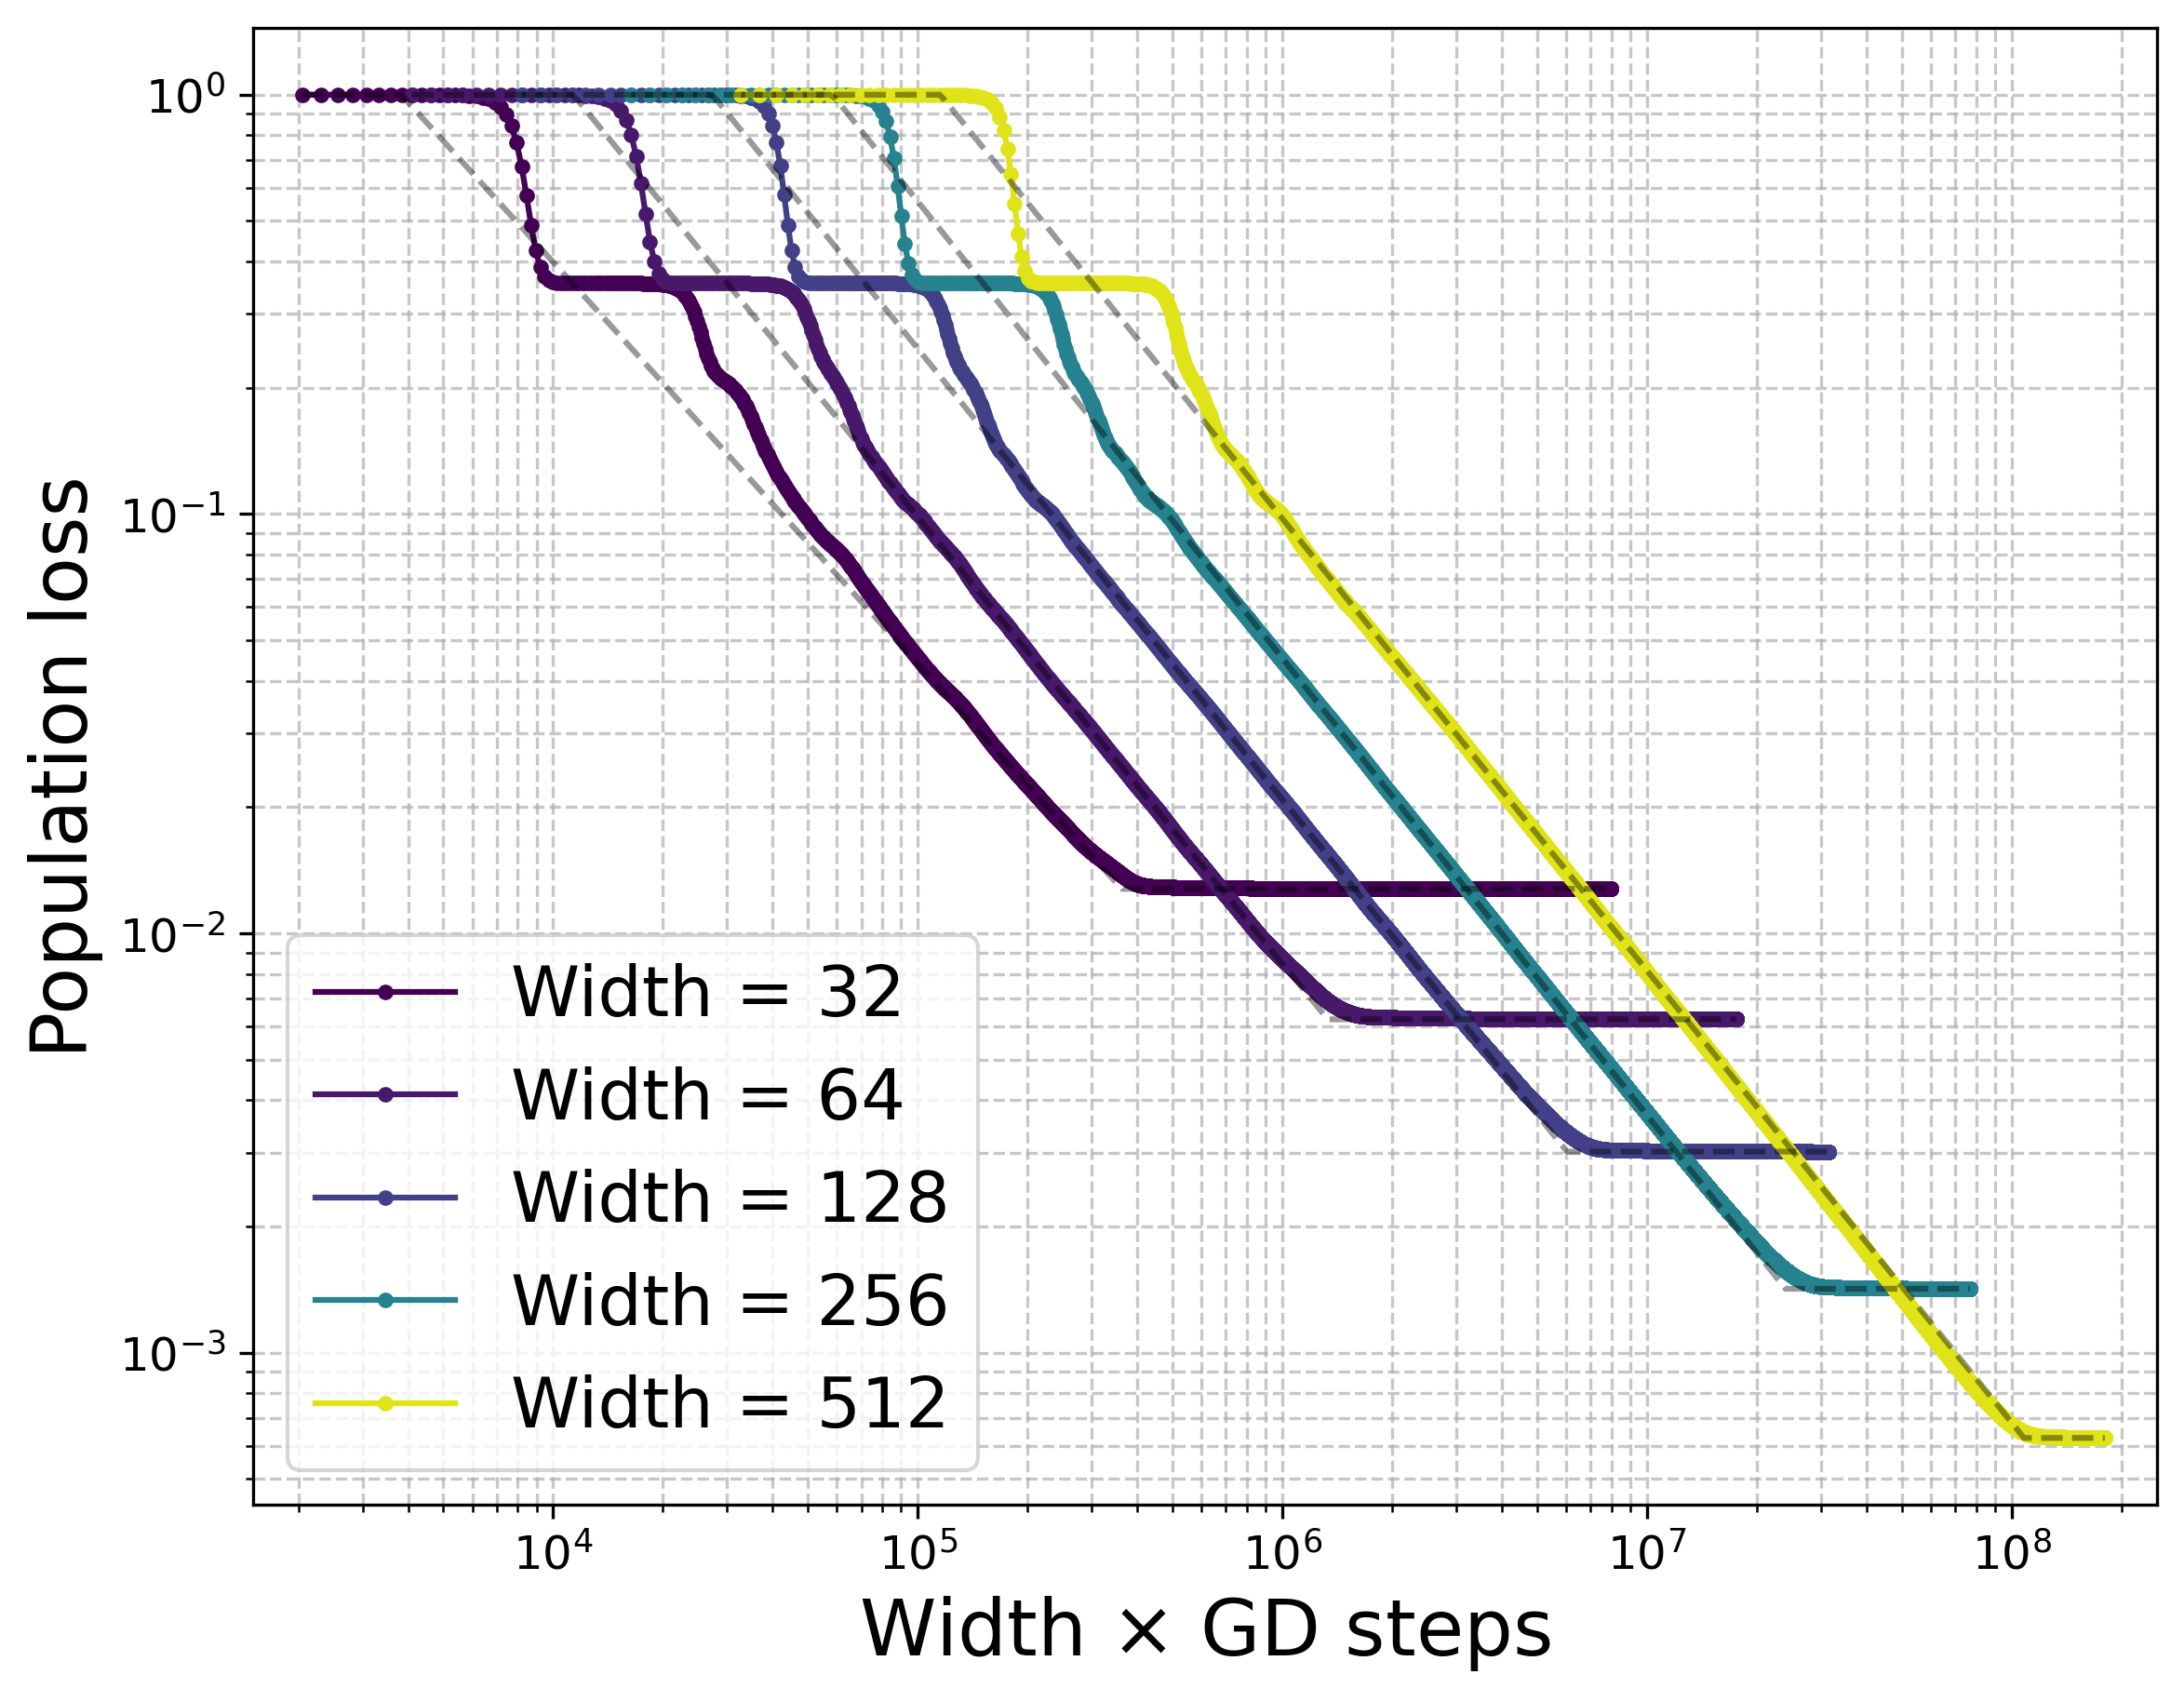
\includegraphics[width=0.95\textwidth]{_figures/__scaling_results_centered_h12_d5000_beta10_ext2.png}
    \caption{$\alpha = 1$. Ideal slope: $-1$, empirical slope:  $-1.08$.\!\!}
    \label{fig:h12a1}
  \end{subfigure}
   ~~~~~~\begin{subfigure}{0.45\textwidth}
   \centering
     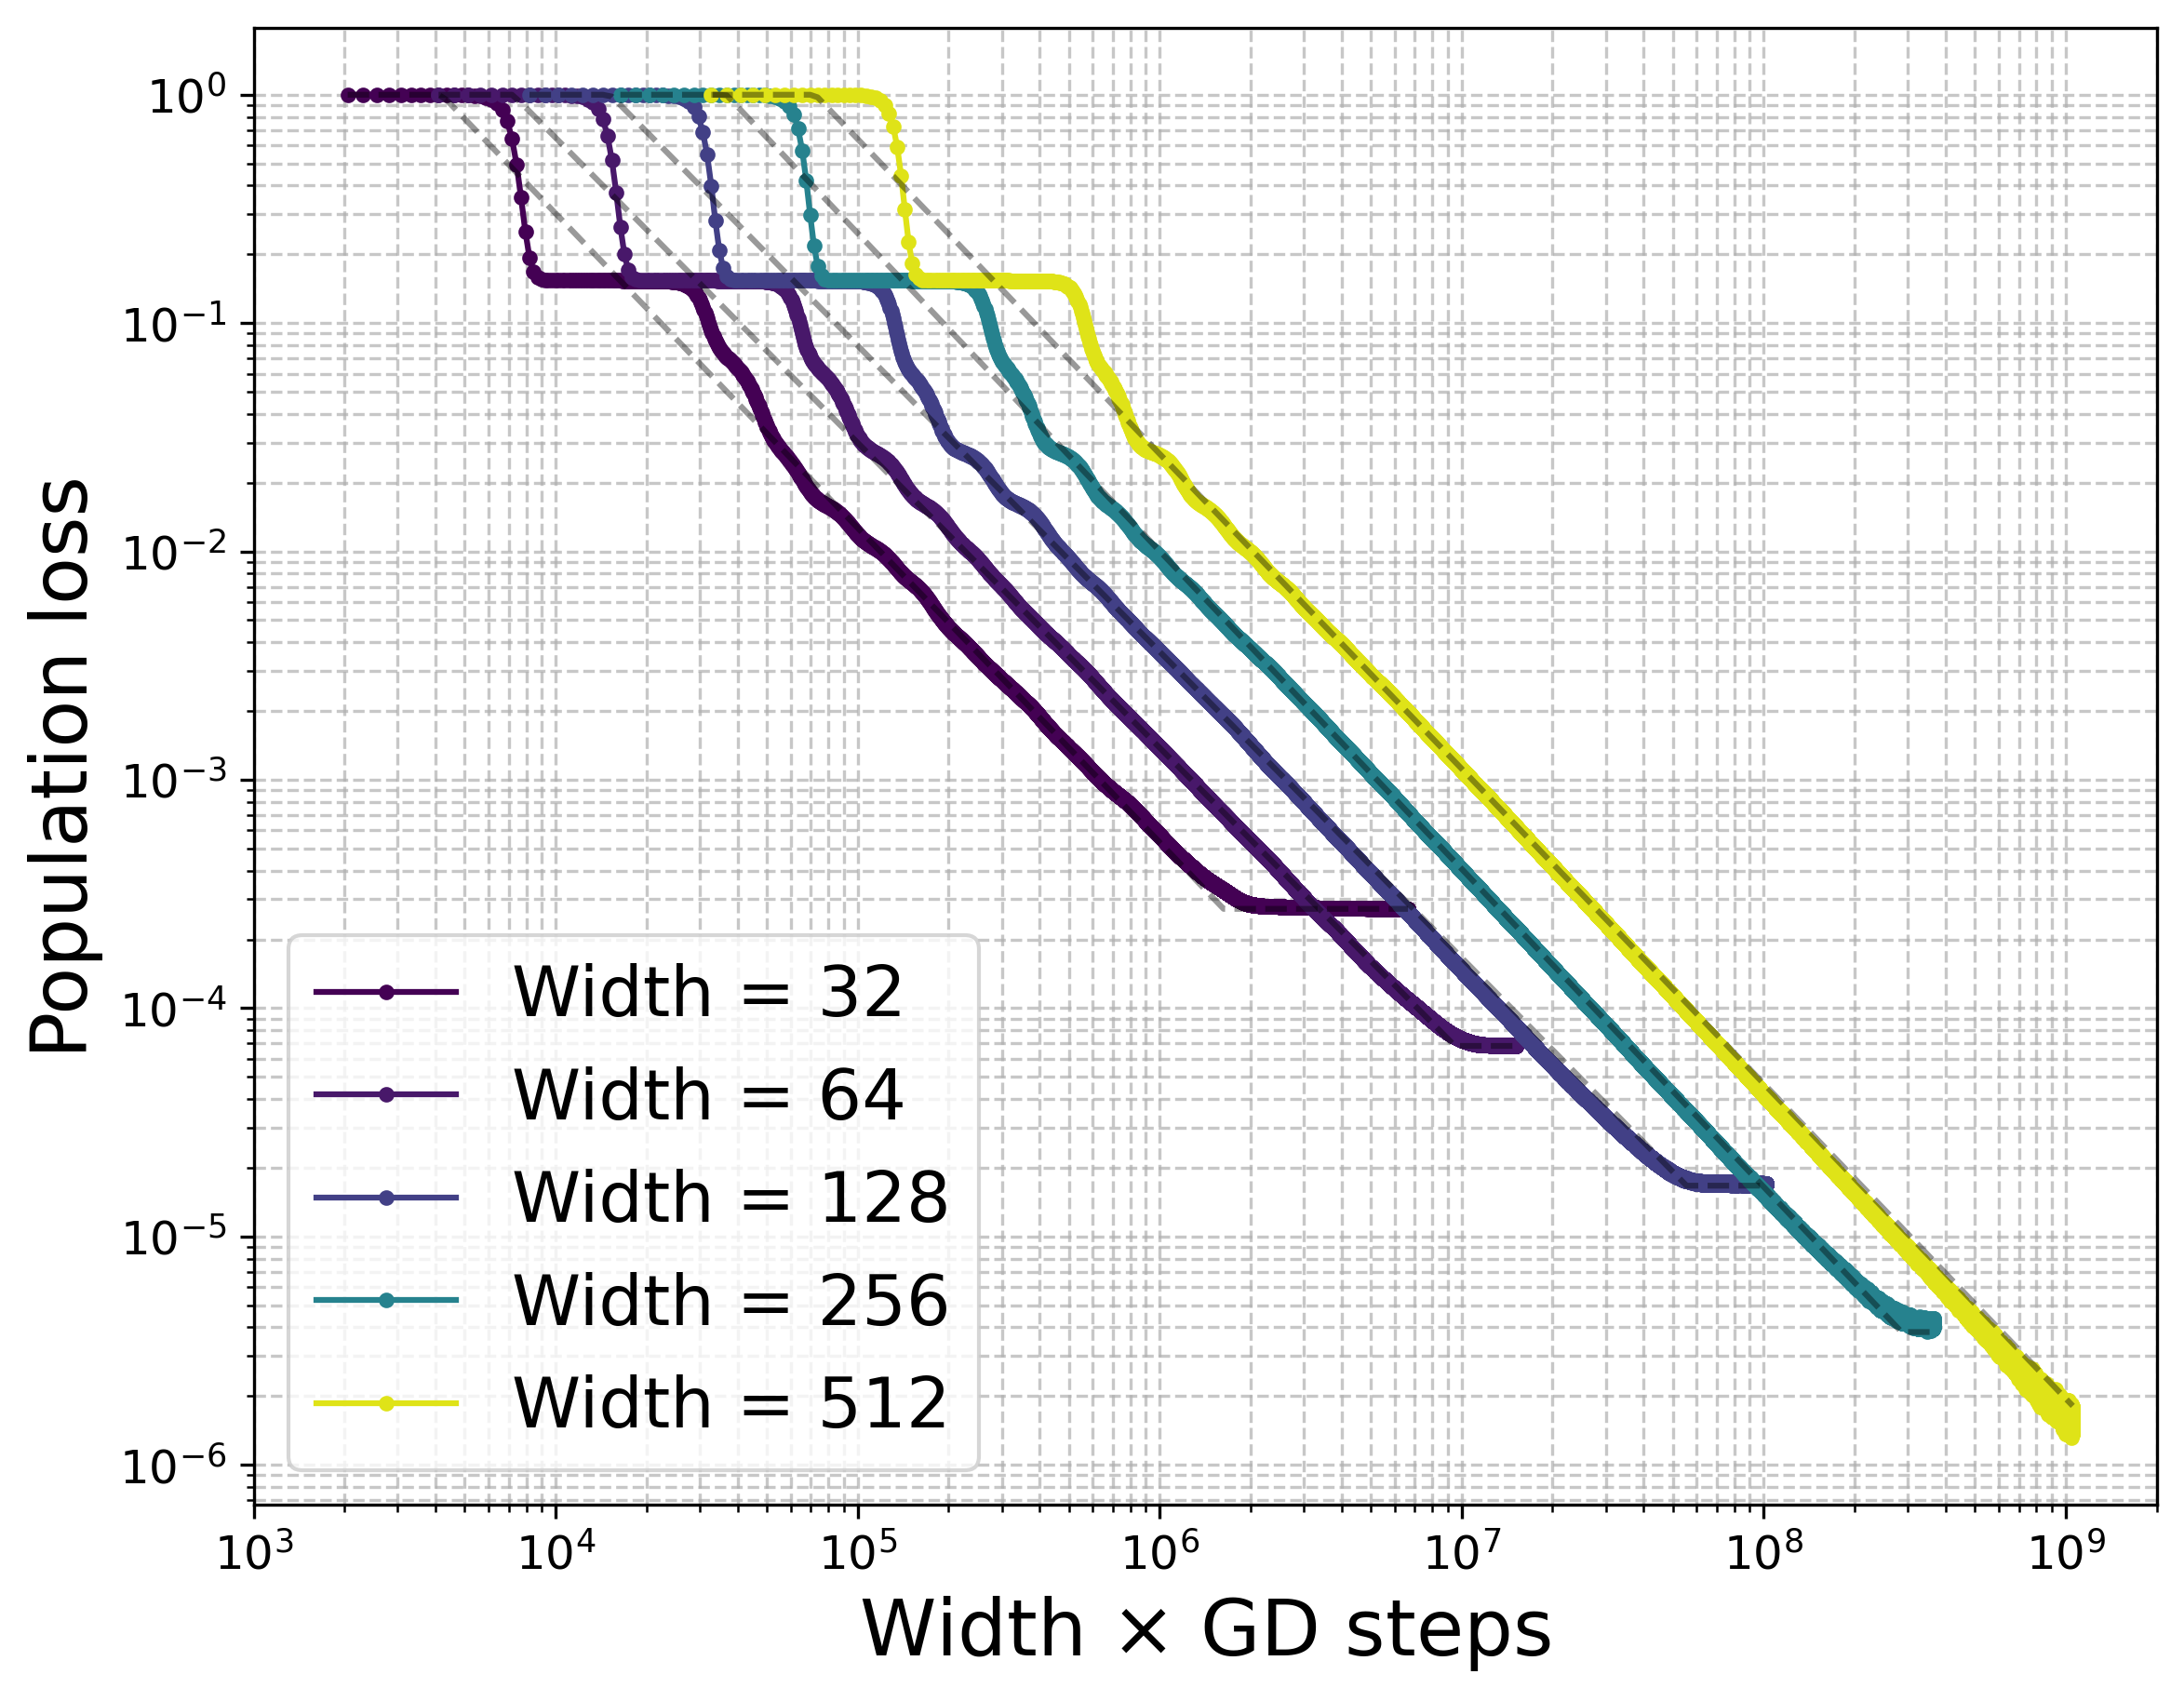
\includegraphics[width=0.95\textwidth]{_figures/__scaling_results_centered_h12_d5000_beta15_ext2.png}
     \caption{$\alpha = \frac{3}{2}$. Ideal slope: $- \frac{4}{3}$, empirical slope:  $-1.38$.\!\!}
    \label{fig:h12a15}
    \end{subfigure}

\caption{\small Population loss vs.~compute for two-layer neural network with activation function $\sigma \propto \mathrm{He}_1 + \mathrm{He}_2$, trained with population gradient descent. The student network adopts the 2-homogeneous parameterization as in \eqref{eq:student}. Observe that after the initial loss drop due to the $\mathrm{He}_1$ component, the risk curves exhibit a power-law scaling where the exponent (dashed lines) nearly matches our theoretical prediction for the quadratic setting $\frac{1-2\alpha}{\alpha}$; and unlike the ReLU setting (Figure \ref{fig:scalinglaw-relu}), the loss immediately plateaus after the power-law phase. } 
  \label{fig:scalinglaw-mixture} 
\end{figure}

\paragraph{Experiment Setting.}  In Figures \ref{fig:scalinglaw-relu}  and \ref{fig:scalinglaw-mixture}, we plot the mean squared error loss for gradient descent with a constant step size on the population loss, using activations $\sigma = \mathrm{ReLU}$ and $\sigma = \mathrm{He}_1 + \mathrm{He}_2$. The teacher model has orthogonal first-layer neurons and power-law decay in the second-layer coefficients with $\alpha \in \{1.0, 1.5\}$. Both teacher and student networks use the same activation function, which we normalize to have zero-mean an unit $L^2$ norm. The student network uses the $2$-homogeneous parameterization:
\eq{
\hat y(\bs{W}) = \frac{1}{\sqrt{\rs}} \sum_{ i = 1}^{\rs} \norm{\bs{w}_i}_2^2 \cdot \sigma(\inner{\bs{w}_i}{\bs{x}}) ~~ \text{where} ~~ \sigma \in  \{ \textstyle \frac{\mathrm{ReLU} - 1/\sqrt{2\pi}}{0.5},  \frac{\mathrm{He}_1 + \mathrm{He}_2}{3}  \}. 
}
We set dimension $d = 5000$, number of teacher neurons $r = 2400$, student widths $\rs \in \{32, 64, 128, 256, 512\}$, and learning rate $\eta =  0.5/\sqrt{r}$.   To estimate the scaling exponents, we first identify the range of compute exhibiting a linear trend by visual inspection, and then fit the exponent via least squares. The dashed lines in the plots correspond to these fitted lines, and the reported empirical exponents represent the median values across different student widths. 

\bigskip


\section{Preliminaries for Proofs}
 \label{sect:prelimproof}
\smallskip

\textbf{Proof organization.}  Section~\ref{sect:prelimproof} introduces the notations and definitions used throughout the paper. In Section~\ref{app:background}, we provide a brief review of matrix Riccati ODEs and difference equations, along with the necessary supporting statements. The main results are proved in Section~\ref{sec:mainproofs}. In Section~\ref{sec:finetuning} we discuss the fine-tuning phase for the discretized algorithm. Additional proofs related to online SGD and auxiliary lemmas are deferred to Sections~\ref{sec:onlinesgd} and~\ref{sec:auxstats}, respectively.

\smallskip
\textbf{Notation and Definitions.}
We use $[n] \coloneqq \{1, 2, \ldots, n\}$ to denote the first $n$ natural numbers. The Euclidean inner product and norm are denoted by $\inner{\cdot}{\cdot}$ and $\norm{\cdot}_2$, respectively.  For matrices, $\norm{\cdot}_2$ and $\norm{\cdot}_\text{F}$ denote the operator norm and Frobenius norm.  The positive part is denoted by $(x)_+ \coloneqq \max\{x, 0\}$. We write $f_d = o_d(1)$ if $f_d \to 0$ as $d \to \infty$, and $f_d \ll g_d$ if $f_d/g_d \to 0$. We use $O(\cdot)$ or $\Omega(\cdot)$ to suppress constants in upper and lower bounds respectively, and we use subscript to indicate parameter dependence, e.g., $O_\alpha(\cdot)$.

\smallskip
 The symmetric part of a square matrix $\bs{M} \in \R^{d \times d}$ is given by $\sym(\bs{M}) \coloneqq \frac{1}{2}(\bs{M} + \bs{M}^\top)$. For symmetric matrices $\bs{A}, \bs{B} \in \R^{d \times d}$, we write $\bs{A} \prec \bs{B}$ (or $\bs{A} \preceq \bs{B}$) if $\bs{B} - \bs{A}$ is positive definite (or positive semidefinite). 
 Moreover, if $\bs{A}$ and $\bs{B}$ are mutually diagonalizable, we write $\bs{A} \bs{B}^{-1} = \frac{\bs{A}}{\bs{B}}$.
 
\smallskip
We follow the convention that subscripts (e.g., $\W_t$) refer to discrete-time quantities, and parentheses (e.g., $\W(t)$) refer to continuous-time quantities. The overlap matrices of interest are defined as
\eq{
\underbrace{ \G_W(t) \coloneqq \W(t) \W(t)^\top }_{\text{Weight Gram matrix}}, \quad 
\underbrace{\G_U(t) \coloneqq \Th^\top \bs{U}(t) \bs{U}(t)^\top \Th }_{\text{Alignment Gram matrix}}, \quad 
\underbrace{\G_t \coloneqq \Th^\top \W_t \W_t^\top \Th. }_{\text{Discrete alignment Gram matrix}}
}

Let $\Z \in \R^{d \times \rs}$ be a Gaussian matrix with i.i.d.\ entries distributed as $\mathcal{N}(0,1/d)$. We define $\Z_{1:m}  \in \R^{m \times \rs}$ as the submatrix formed by the first $m$ rows:
\eq{
\Z = \begin{bmatrix}
\Z_{1:m} \\
\Z_{\text{rest}}
\end{bmatrix}.
}
Without loss of generality, we assume the teacher directions coincide with the standard basis vectors, i.e., $\bs{\theta}_j = \bs{e}_j$. With this, the initialization satisfies:
\eq{
\G_W(0) = \Z \Z^\top, \qquad 
\G_U(0) = \G_0 = \Z_{1:r} (\Z^\top \Z)^{-1} \Z_{1:r}^\top.  \label{def:init}
}
We start with characterizing ``good events'' for initial matrices given by the following lemma:
\begin{lemma}
\label{lem:goodevents}
\hfill \\[0.6em]
\textbf{Both cases ($\alpha \in [0,0.5) \cup (0.5,\infty)$).}  For $d \geq \Omega(1)$, the following holds:
\begin{enumerate}[label=(E.\arabic*)]
\item   \label{event:Zbound}    $ \tfrac{1}{1.05} \leq \lambda_{\mathrm{min}} (\Z^\top \Z  ) \leq \lambda_{\mathrm{max}} (  \Z^\top \Z) \leq 1.05$.
\item   \label{event:Gbound}  $  1.05 \Z_{1:r} \Z_{1:r}^\top \succeq \G_U(0) = \G_0 \succeq       \frac{1}{1.05} \Z_{1:r} \Z_{1:r}^\top$.
\end{enumerate}
\textbf{Heavy-tailed case ($\alpha \in [0,0.5)$).}   For $d \geq \Omega_{\varphi}(1)$, the following holds:
\begin{enumerate}[label=(H.\arabic*)]
\item \label{event:htZlb}  For  $m  \leq  \rs (1 -   \log^{\nicefrac{-1}{2}} d) \wedge r$ uniformly,  we consider $\lambda_{\mathrm{min}} (  \Z_{1:m} \Z_{1:m}^\top ) \geq  \tfrac{\rs}{5 d} \big( 1 -  \tfrac{m}{\rs}   \big)^2 $.
\item \label{event:htZlbiso}  For all $m  \leq  \rs (1 -   \log^{\nicefrac{-1}{2}} d) \wedge r$ uniformly,  $\lambda_{m}(    \Z_{1:r} \Z_{1:r}^\top ) \geq  \tfrac{\rs}{5 d} \big( 1 -     \tfrac{m}{\rs}    \big)^2$.
\item \label{event:htZub}    $\lambda_{\mathrm{max}} ( \Z_{1:r} \Z_{1:r}^\top ) \leq \frac{2\rs}{d} \big(1 + \frac{1}{\sqrt{\varphi}} \big)^2$.
\end{enumerate}
\textbf{Light-tailed case ($\alpha \in [0,0.5)$).}   For $d \geq \Omega(1)$, the following holds:
\begin{enumerate}[label=(L.\arabic*)]
\item   \label{event:ltZlb}  $\tfrac{1}{\rs^5 d}  \leq  \lambda_{\mathrm{min}} (  \Z_{1:\rs} \Z_{1:\rs}^\top )$
\item   \label{event:ltZub}   For   $m  \in \{ 1, 2, \cdots, 5 \rs,  \ceil{\log^{2.5} d},\ceil{\log^{6} d}, r \}$ uniformly,  $ \lambda_{\mathrm{max}} ( \Z_{1:m} \Z_{1:m}^\top ) \leq  \tfrac{5(\rs\vee m)}{d}$
\end{enumerate}
We define
\eq{
\mathcal{G}_{\text{init}} \equiv \begin{cases}
  \ref{event:Zbound}  \cap \ref{event:Gbound} \cap   \ref{event:htZlb}  \cap  \ref{event:htZlbiso}   \cap   \ref{event:htZub} , & \alpha \in [0,0.5) \\
    \ref{event:Zbound}  \cap \ref{event:Gbound} \cap   \ref{event:ltZlb} \cap    \ref{event:ltZub} , & \alpha \in > 0.5.
\end{cases}
}
We have 
\eq{
\mpr[ \mathcal{G}_{\text{init}} ] \geq \begin{cases}
 1 - 3  \rs \exp \big( \tfrac{- \rs}{2 \log^2  d} \big)  , & \alpha \in [0,0.5) \\
1 - \Omega(1/\rs^2), & \alpha  > 0.5.
\end{cases}
}
\end{lemma}
 
 \begin{proof}
We will use the following:
\begin{enumerate}[label=(S.\arabic*), leftmargin=*]
\item   \label{cond:lowerbound} By \cite[Corollary 5.35]{vershynin2010introduction},   for $m \leq \rs$ and $\sqrt{\rs} - \sqrt{m} \geq t > 0$ 
\eq{
& \mpr \left[      \lambda_{\mathrm{min}} \left(  \bs{Z}_{1:m} \bs{Z}_{1:m}^\top  \right) \! \geq \!   \tfrac{\rs}{d}  \left( 1 \! - \! \sqrt{  \tfrac{m}{\rs}  } \! - \! \tfrac{t}{\sqrt{\rs}} \right)^2 \right] \geq 1 - 2 e^{- t^2}, 
}
and   for  $m \geq \rs$ and $\sqrt{m} - \sqrt{\rs} \geq t > 0$ 
\eq{
& \mpr \left[      \lambda_{\mathrm{min}} \left( \bs{Z}_{1:m}^\top  \bs{Z}_{1:m}   \right) \! \geq \!   \tfrac{m}{d}  \left( 1 \! - \! \sqrt{  \tfrac{\rs}{m}  } \! - \! \tfrac{t}{\sqrt{m}} \right)^2 \right] \geq 1 - 2 e^{- t^2}.  
}

\item  \label{cond:upperbound}	By \cite[Corollary 5.35]{vershynin2010introduction},  for any fixed $m$  
\eq{
\mpr \left[  \tfrac{m}{d} \left( 1 + \sqrt{  \tfrac{\rs}{m}  } + \tfrac{t}{\sqrt{m}} \right)^2 \geq \lambda_{\mathrm{max}} \left(  \bs{Z}_{1:m}^\top   \bs{Z}_{1:m} \right)   \right] \geq 1 - 2 e^{- t^2}.
}
\item  \label{cond:squarematrix} By \cite[Theorem 5.38]{vershynin2010introduction}, there exists $C, c > 0$ such that
\eq{
\mpr \left[     \lambda_{\mathrm{min}} \left(  \bs{Z}_{1:\rs} \bs{Z}_{1:\rs}^\top  \right)\geq \tfrac{  \varepsilon^2}{4 d \rs}  \right] \geq 1 -  C \varepsilon -  e^{- c \rs}.
}
\end{enumerate}
For the heavy tailed case,  we  consider $d$ is large enough to guarantee  $\abs{\tfrac{\rs}{r} - \varphi} \leq \frac{\varphi}{2}.$ We have
\begin{itemize}[leftmargin=*]
\item  By using \ref{cond:lowerbound} and \ref{cond:upperbound} with $m = d$,  $t = \sqrt{ \tfrac{d}{\log d} }$, we can show that $\mpr[  \ref{event:Zbound} ] \geq 1 - e^{ \frac{ - d}{\log d}}$ for $d \geq \Omega(1)$.
 \item By   \eqref{def:init} and   \ref{event:Zbound} ,    \ref{event:Gbound}  follows.
 \item For   \ref{event:htZlb}, by using \ref{cond:lowerbound} with $t = \frac{\sqrt{\rs} - \sqrt{m}}{\sqrt{\log d}} \geq  \sqrt{  \tfrac{\rs }{2 \log^2 d} }$, we have with probability $1 - 2 \rs \exp \big( \tfrac{- \rs}{2 \log^2  d} \big)$,   for $m \leq \rs (1 -   \log^{\nicefrac{-1}{2}} d) \wedge r$ uniformly:
\eq{
 \lambda_{\mathrm{min}} \left(  \bs{Z}_{1:m} \bs{Z}_{1:m}^\top  \right) >   \tfrac{\rs}{d} \left( 1 - \tfrac{1}{\sqrt{\log d}} \right)^2    \left( 1  - \sqrt{  \tfrac{m}{\rs}  }  \right)^2 \geq  \tfrac{\rs}{5 d}  \left( 1  -   \tfrac{m}{\rs}   \right)^2 . 
}
Therefore,   $\mpr[  \ref{event:htZlb} ] \geq 1 - 2 \rs \exp \big( \tfrac{- \rs}{2 \log  d} \big)$.
\item By Cauchy's eigenvalue interlacing theorem,   $\lambda_{m}(    \Z_{1:r} \Z_{1:r}^\top ) \geq  \lambda_{\mathrm{min}} \left(  \bs{Z}_{1:m} \bs{Z}_{1:m}^\top  \right)$. Therefore, by  \ref{event:htZlb} ,  \ref{event:htZlbiso} follows. 
\item For \ref{event:htZub} , by using $m = r$ and $t = 0.4 \sqrt{\rs}$ in   \ref{cond:upperbound}, we have 	 $\mpr[  \ref{event:htZub}  ] \geq 1 - 2 e^{- 0.16 \rs}$.
\item  For   \ref{event:ltZlb}, by using \ref{cond:squarematrix} with $\varepsilon = \frac{2}{\rs^2}$,  we have  $\mpr  [   \ref{event:ltZlb} ] \geq 1 - \Omega(1/\rs^2)$.
\item  For   \ref{event:ltZub},  by using  \ref{cond:upperbound}  with $t = 0.4 \sqrt{\rs}$, we have with probability $1 -  (10 \rs + 6) e^{-0.16 \rs}$ for $m \in [5\rs] \cup \{\ceil{\log^{2.5} d} ,\ceil{\log^{6} d}, r \}$ uniformly:
\eq{
 \lambda_{\mathrm{max}} ( \Z_{1:m} \Z_{1:m}^\top ) \leq   \tfrac{\rs}{d} \left( 1.4 + \sqrt{  \tfrac{m}{\rs}  }  \right)^2 \leq \frac{5 (\rs \vee m)}{d}.
}
\end{itemize}
By union bound, we have the result.
 \end{proof}


 

\section{Background: Matrix Riccati Dynamical Systems}
\label{app:background}
We begin by reviewing Riccati dynamical systems in both continuous and discrete time, establishing the necessary background for the arguments that follow. For the following, we define
\eq{
 \Lae \coloneqq \begin{bmatrix}
 \bs{\Lambda}  & 0 \\
0 & 0
\end{bmatrix} ~~ \text{and} ~~   \tL \coloneqq 
 \tfrac{\sqrt{\rs}}{\normL}   \Lae.
}
For notational convenience,     we adapt the abuse of notation:
\eq{
\frac{ \Lae}{\bs{I}_d - \exp (   - t   \Lae)} = \lim_{\varepsilon \to 0}  \frac{ (    \Lae  + \varepsilon \bs{I}_d)}{\bs{I}_d - \exp (  - t (  \Lae  + \varepsilon \bs{I}_d) )}  =   \begin{bmatrix}
\frac{        \bs{\Lambda}  }{\bs{I}_r - \exp (    - t      \bs{\Lambda}  )} & 0 \\ 
0 &   \frac{1}{t} \bs{I}_{d - r}
\end{bmatrix}.
}
\subsection{Continous-time Matrix Riccati ODE}
In this paper, we study continuous-time matrix Riccati differential equations of the following form:
\begin{itemize}[leftmargin=*]
\item Weight Gram matrix: For  $T_W = \rs$
\eq{
\partial_t  \G_{W}(t) =  \frac{0.5}{T_W}   \Big( \tL \G_{W}(t)  + \G_{W}(t)  \tL -  2   \G^2_{W}(t)     \Big). \label{def:weightGramode}
}
\item   Alignment Gram matrix:  For $T_U = \normL \sqrt{\rs}$, 
\eq{
\partial_t  \G_{U}(t) =  \frac{0.5}{T_U}   \Big( \La \G_{U}(t)  + \G_{U}(t)   \La -  2   \G_{U}(t)  \La \G_{U}(t)     \Big). \label{def:alignmentGramode}
}
\end{itemize}
 
For $\alpha = 0$, we assume that the ODEs are expressed in the eigenbasis of $\G_W(0)$ or $\G_U(0)$, ensuring that the trajectories remain diagonal. The solutions of these ODEs are characterized in the following statement:

\begin{lemma} 
\label{lem:riccsolution}
\eqref{def:weightGramode}  and \eqref{def:alignmentGramode} admit the following solutions:
\eq{
\bs{G}_W(t) & = 
    \frac{  \tL}{\bs{I}_d   -   \exp  (  \nicefrac{-  t \tL}{T_W}  )}   -  \frac{     \tL  \exp (  \nicefrac{- 0.5 t \tL}{T_W} ) }{\bs{I}_d  -  \exp (  \nicefrac{-  t \tL}{T_W} )}     \bigg (\G_{W}(0)  +   \frac{    \tL  \exp  (  \nicefrac{-   t \tL}{T_W} ) }{\bs{I}_d \! - \! \exp  (  \nicefrac{-  t \tL}{T_W} )}    \bigg )^{-1}     \frac{  \tL  \exp (  \nicefrac{- 0.5 t \tL}{T_W} ) }{\bs{I}_d \! - \! \exp (    \nicefrac{- t \tL}{T_W}  )}  \\[0.6em]
    \bs{G}_U(t) &  = 
    \frac{  \bs{I}_r }{\bs{I}_r - \exp  (  \nicefrac{-  t \La}{T_U}  )} \!  - \! \frac{      \exp (  \nicefrac{- 0.5 t \La}{T_U} ) }{\bs{I}_r - \exp (  \nicefrac{-  t \La}{T_U} )}     \bigg (\G_{U}(0)  +     \frac{      \exp (  \nicefrac{-   t \La}{T_U} ) }{\bs{I}_r - \exp (  \nicefrac{-  t \La}{T_U} )}      \bigg )^{-1}   \frac{      \exp (  \nicefrac{- 0.5 t \La}{T_U} ) }{\bs{I}_r - \exp (  \nicefrac{-  t \La}{T_U} )}    
}
Moreover,    $( \G_{W}(t) )_{t \geq 0}$ and   $(\G_{U}(t) )_{t \geq 0}$ are monotone with respect to  $\G_{W}(0)  \succeq 0$ and $\G_{U}(0)  \succeq 0$ respectively.
\end{lemma}

\begin{proof}
 One can check by direct differentiation that the given closed-form expressions satisfy the ODEs above. The uniqueness of the solutions follow the local Lipschitzness of the drifts. Monotonicity is a consequence of Proposition \ref{prop:monotonecharac}.
\end{proof}
 


\subsection{Discrete-time Matrix Riccati Difference Equations}
In this section, we will study a particular discretization of Alignment Gram matrix ODE, given as
\eq{
\G_{t+1} = \G_t   - \frac{\eta}{2}  (2 \G_t - \bs{I}_r) \La  (2 \G_t - \bs{I}_r)  \big(\bs{I}_r + \eta \La  (2 \G_t - \bs{I}_r) \big)^{-1} + \eta   \bs{\Lambda}. \label{eq:discreteupdate}
}
For convenience, we will make a change of variable and define $\V_t \coloneqq   2 \La^{\frac{1}{2}} \G_t  \La^{\frac{1}{2}}  - \La$. We write  \eqref{eq:discreteupdate} in terms of $\V_t$ as follows:
\eq{
\V_{t+1} =   \V_t   - \eta \V_t^2  \big(\bs{I}_r + \eta   \V_t \big)^{-1} + \eta   \bs{\Lambda}^2. \label{eq:discreteupdat2}
}
We characterize the dynamics of $(\V_t)_{t \in \N}$ as follows:



\begin{lemma}
\label{lem:discretericcati2}
We consider
\eq{
\begin{bmatrix} 
\bs{X}_{t+1,1} \\
\bs{X}_{t+1,2}
\end{bmatrix} =  \begin{bmatrix} 
\bs{X}_{t, 1}  \\
\bs{X}_{t, 2} 
\end{bmatrix}  + \eta \bs{H}
\begin{bmatrix} 
\bs{X}_{t, 1} \\
\bs{X}_{t, 2}
\end{bmatrix} ~~ \text{where} ~~
\begin{bmatrix} 
\bs{X}_{0,1} \\
\bs{X}_{0,2}
\end{bmatrix} =
\begin{bmatrix} 
\bs{I}_r \\
\bs{V}_0
\end{bmatrix}   ~ \text{and} ~ \bs{H} \coloneqq \begin{bmatrix}
0 &  \bs{I}_r \\ 
 \bs{\Lambda}^2 &   \eta  \bs{\Lambda}^2
\end{bmatrix}.
}

The following hold for all $n \in \N$:
\begin{enumerate}[label=(R.\arabic*), leftmargin=*]
\item \label{res:posdef} We have
\eq{
\begin{bmatrix}
\bs{A}_{t,11} & \bs{\Lambda}^{-1} \bs{A}_{t,12} \\
 \bs{\Lambda}  \bs{A}_{t,12} & \bs{A}_{t,22}
\end{bmatrix} \coloneqq (\bs{I}_{2r} + \eta   \bs{H})^t.    \label{eq:matrixpowerform}
} 
where $\bs{A}_{t,11}$,  $\bs{A}_{t,12}$,  $\bs{A}_{t,22}$ are positive definite diagonal matrices.
\item \label{res:symdet} $\bs{A}_{t,11} + \eta \bs{\Lambda} \bs{A}_{t,12} = \bs{A}_{t,22}$ and $\bs{A}_{t,22} \bs{A}_{t,11} -  \bs{A}_{t,12}^2  = \bs{I}_r$.
\item  \label{res:ratiolb} For $\eta \leq 1$, we have  $\bs{A}_{t,11} \bs{A}_{t,12}^{-1} \succ \big( \bs{I}_r + \tfrac{\eta^2}{4} \bs{\Lambda}^2 \big)^{1/2} - \tfrac{\eta}{2}  \bs{\Lambda}$ and $\bs{A}_{t,22} \bs{A}_{t,12}^{-1} \succ \big( \bs{I}_r + \tfrac{\eta^2}{4} \bs{\Lambda}^2 \big)^{1/2} + \tfrac{\eta}{2}  \bs{\Lambda}$.
\item  \label{res:ratiobound} If $\norm{\eta \bs{\Lambda} }_2 < 1$,  
\eq{
\bs{A}_{t,22} \bs{A}_{t,12}^{-1} \succ \frac{(\bs{I}_r + \eta \bs{\Lambda})^t +(\bs{I}_r - \eta \bs{\Lambda})^t  }{(\bs{I}_r + \eta \bs{\Lambda})^t  - (\bs{I}_r - \eta \bs{\Lambda})^t  } \succeq \bs{A}_{t,11} \bs{A}_{t,12}^{-1}.
}
\end{enumerate}
Moreover, if $\bs{X}_{t,1}$ and $\bs{X}_{t+1,1}$ are invertible:
\begin{enumerate}[label=(R.\arabic*), leftmargin=*]
\setcounter{enumi}{6}
\item  \label{res:update}  For $\bs{V}_{t+1} \coloneqq  \bs{X}_{t+1,2} \bs{X}_{t+1,1}^{-1}$, and $\bs{V}_t \coloneqq  \bs{X}_{2,t} \bs{X}_{t,1}^{-1}$, we have
\eq{
\bs{V}_{t+1}  = \bs{V}_t - \eta  \bs{V}_t^2   \left(\bs{I}_r +   \eta \bs{V}_t \right )^{-1} +  \eta  \bs{\Lambda}^2. 
}
\end{enumerate}
\end{lemma} 





\begin{proof}[Proof of Lemma \ref{lem:discretericcati2}]
We have
\eq{
\bs{I}_{2r} + \eta   \bs{H}  = \begin{bmatrix}
\bs{I}_r & \eta \bs{I}_r \\
\eta \bs{\Lambda}^2 & \bs{I}_r + \eta^2 \bs{\Lambda}^2
\end{bmatrix}. \label{def:updmatrix}
}
Let
\eq{
(\bs{I}_{2r} + \eta   \bs{H})^t \eqqcolon \begin{bmatrix}
\bs{\tilde{A}}_{t,11} & \bs{\tilde{A}}_{t,12} \\
\bs{\tilde{A}}_{21,t} & \bs{\tilde{A}}_{t,12}
\end{bmatrix}.  \label{eq:matrixpower}
}
Since each submatrix  in \eqref{def:updmatrix} is diagonal positive definite,  the matrices in  \eqref{eq:matrixpowerform} are also diagonal positive definite.  To prove \ref{res:posdef} and the first part of \ref{res:symdet}  we use proof by induction.  We assume   $\bs{\tilde{A}}_{t,11} + \eta \bs{\tilde{A}}_{21, t} = \bs{\tilde{A}}_{t,12}$ and  $\bs{\tilde{A}}_{21, t} \bs{\tilde{A}}^{-1}_{12, t} = \bs{\Lambda}^2$.
We have
\eq{
 \bs{\tilde{A}}_{12, t+1} =  \bs{\tilde{A}}_{t,12}  + \eta   \bs{\tilde{A}}_{t,12}
  \labelrel={ricc:eqq0}   \bs{\tilde{A}}_{t,12}   + \eta \left( \bs{\tilde{A}}_{t,11} + \eta \bs{\tilde{A}}_{21, t}  \right)  
& \labelrel={ricc:eqq1}   \eta \bs{\tilde{A}}_{t,11} + \left( \bs{I}_r + \eta^2   \bs{\Lambda}^2 \right)     \bs{\tilde{A}}_{t,12}  \\
& \labelrel={ricc:eqq2}   \eta \bs{\tilde{A}}_{t,11} + \bs{\Lambda}^{-2}  \left( \bs{I}_r + \eta^2   \bs{\Lambda}^2 \right)     \bs{\tilde{A}}_{21, t}     \\
& =   \bs{\Lambda}^{-2}   \bs{\tilde{A}}_{21, t+1} .
}
where  \eqref{ricc:eqq0}  follows the first assumption, \eqref{ricc:eqq1}  and \eqref{ricc:eqq2} follow the second assumption. 
Moreover,
\eq{
\bs{\tilde{A}}_{11, t+1} + \eta \bs{\tilde{A}}_{21, t+1} & =  \bs{\tilde{A}}_{t,11} + \eta \bs{\tilde{A}}_{21, t} + \eta^2 \bs{\Lambda}^2    \bs{\tilde{A}}_{t,11} + \eta (\bs{I}_r + \eta^2 \bs{\Lambda}^2)  \bs{\tilde{A}}_{21, t}  \\
& =  (\bs{I}_r + \eta^2 \bs{\Lambda}^2)  (  \bs{\tilde{A}}_{t,11} + \eta \bs{\tilde{A}}_{21, t}  ) + \eta  \bs{\tilde{A}}_{21, t}  \\
&  \labelrel={ricc:eqq3}  (\bs{I}_r + \eta^2 \bs{\Lambda}^2)   \bs{\tilde{A}}_{t,12}  +   \eta \bs{\Lambda}^2  \bs{\tilde{A}}_{t,12}   
  =   \bs{\tilde{A}}_{22, t+1}. 
}
where \eqref{ricc:eqq3}  follows the first and second assumptions. For the second part of  \ref{res:symdet}  we again use proof by induction.  We assume 
$\bs{A}_{t,22} \bs{A}_{t,11} -  \bs{A}_{t,12}^2  = \bs{I}_r$.  We have
\eq{
  \bs{\tilde{A}}_{11, t+1}   \bs{\tilde{A}}_{22, t+1}   -  \bs{\tilde{A}}_{12, n+1}   \bs{\tilde{A}}_{21, t+1}  
  & = \Big(   \bs{\tilde{A}}_{t,11} + \eta  \bs{\tilde{A}}_{21, t}  \Big) \Big( \eta \bs{\Lambda}^2  \bs{\tilde{A}}_{t,12}   + \left( \bs{I}_r + \eta^2 \bs{\Lambda}^2 \right)  \bs{\tilde{A}}_{t,12} \Big) \\
  & - \Big( \eta \bs{\Lambda}^2  \bs{\tilde{A}}_{t,11} +   \left( \bs{I}_r + \eta^2 \bs{\Lambda}^2 \right)  \bs{\tilde{A}}_{21, t}   \Big) \Big( \bs{\tilde{A}}_{t,12}  + \eta \bs{\tilde{A}}_{t,12} \Big) \\
  & =    \bs{\tilde{A}}_{t,11}   \bs{\tilde{A}}_{t,12}  -  \bs{\tilde{A}}_{t,12}    \bs{\tilde{A}}_{21, t} = \bs{I}_r.
}
For   \ref{res:ratiolb}, by using  \ref{res:symdet},  we have
\eq{
 \bs{A}_{t,11} \left(  \bs{A}_{t,11} + \eta \bs{\Lambda} \bs{A}_{t,12}    \right)  -  \bs{A}_{t,12}^2  = \bs{I}_r &  \Rightarrow \big(\bs{A}_{t,11} \bs{A}^{-1}_{t,12} \big)^2 + \eta \bs{\Lambda}  \big(\bs{A}_{t,11} \bs{A}^{-1}_{t,12} \big) - \bs{I}_r \succ 0 \\
&  \Rightarrow \bs{A}_{t,11} \bs{A}^{-1}_{t,12} \succ  \left( \bs{I}_r + \frac{\eta^2}{4}  \bs{\Lambda}  \right)^{1/2}  -  \frac{\eta}{2} \bs{\Lambda}.
}
The second part follows   \ref{res:symdet}.  For \ref{res:ratiobound}, we recall that
\eq{
& \bs{A}_{t+1,12} = \bs{A}_{t,12} + \eta \bs{\Lambda} \bs{A}_{t,22}  =  (\bs{I}_r + \eta^2 \bs{\Lambda}^2)\bs{A}_{t,12} + \eta \bs{\Lambda} \bs{A}_{t,11}  \label{eq:riccfact1} \\
& \bs{A}_{t+1,22} = \eta   \bs{\Lambda}  \bs{A}_{t,12} + \left( \bs{I}_r + \eta^2 \bs{\Lambda}^2 \right)  \bs{A}_{t,22} \succ \eta   \bs{\Lambda}  \bs{A}_{t,12} + \bs{A}_{t,22}.  \label{eq:riccfact2}  
% & \bs{A}_{11, n+1} =  \bs{A}_{t,11} + \eta   \bs{\Lambda}  \bs{A}_{t,12}. \label{eq:riccfact3}
}
We use proof by induction.  Suppose the lower bound for $\tfrac{\bs{A}_{t,22}}{\bs{A}_{t,12}}$ holds.  We have
\eq{
\frac{\bs{A}_{t+1,22}}{\bs{A}_{t+1,12}} & \labelrel\succ{ricc:ineqq4} \frac{\eta   \bs{\Lambda}  \bs{A}_{t,12} + \bs{A}_{t,22} }{\bs{A}_{t,12} + \eta \bs{\Lambda} \bs{A}_{t,22}}   \\
 &  \labelrel\succ{ricc:ineqq5} \left( \eta   \bs{\Lambda}  +  \frac{(\bs{I}_r + \eta \bs{\Lambda})^t +(\bs{I}_r - \eta \bs{\Lambda})^t  }{(\bs{I}_r + \eta \bs{\Lambda})^t  - (\bs{I}_r - \eta \bs{\Lambda})^t } \right) \left(  \bs{I}_r + \eta \bs{\Lambda}   \frac{(\bs{I}_r + \eta \bs{\Lambda})^t +(\bs{I}_r - \eta \bs{\Lambda})^t  }{(\bs{I}_r + \eta \bs{\Lambda})^t  - (\bs{I}_r - \eta \bs{\Lambda})^t  } \right)^{-1}   \\[0.5em]
& =  \frac{(\bs{I}_r + \eta \bs{\Lambda})^{t+1}  +(\bs{I}_r - \eta \bs{\Lambda})^{t+1}  }{(\bs{I}_r + \eta \bs{\Lambda})^{t+1}  - (\bs{I}_r - \eta \bs{\Lambda})^{t+1}  }.
}
where \eqref{ricc:ineqq4} follows \eqref{eq:riccfact2} and  \eqref{ricc:ineqq5} follows the induction hypothesis with that  $x \to \frac{x + \eta \lambda}{1+ \eta \lambda x}$ is monotonic increasing for $\eta \lambda < 1$.  For the upper bound,   suppose the lower bound for $\tfrac{\bs{A}_{t,11}}{\bs{A}_{t,12}}$ holds. We have
\eq{
\frac{\bs{A}_{t+1,11}}{\bs{A}_{t+1,12}} & \labelrel\preceq{ricc:ineqq6} \frac{\bs{A}_{t,11} + \eta   \bs{\Lambda}  \bs{A}_{t,12}}{\bs{A}_{t,12} + \eta \bs{\Lambda} \bs{A}_{t,11}}
 \\
 &  \labelrel\preceq{ricc:ineqq7} \left( \eta   \bs{\Lambda}  +  \frac{(\bs{I}_r + \eta \bs{\Lambda})^t +(\bs{I}_r - \eta \bs{\Lambda})^t  }{(\bs{I}_r + \eta \bs{\Lambda})^t  - (\bs{I}_r - \eta \bs{\Lambda})^t  } \right) \left( \bs{I}_r + \eta \bs{\Lambda}   \frac{(\bs{I}_r + \eta \bs{\Lambda})^t +(\bs{I}_r - \eta \bs{\Lambda})^t  }{(\bs{I}_r + \eta \bs{\Lambda})^t  - (\bs{I}_r - \eta \bs{\Lambda})^t  } \right)^{-1}   \\[0.5em]
& =  \frac{(\bs{I}_r + \eta \bs{\Lambda})^{t+1}  +(\bs{I}_r - \eta \bs{\Lambda})^{t+1}  }{(\bs{I}_r + \eta \bs{\Lambda})^{t+1}  - (\bs{I}_r - \eta \bs{\Lambda})^{t+1}  }.
}
where \eqref{ricc:ineqq6} follows \eqref{eq:riccfact1},  and \eqref{ricc:ineqq7} follows the induction hypothesis. 

Lastly if  $\bs{X}_{t,1}$ and  $\bs{X}_{t+1,1}$ are invertible,
\eq{
 \bs{X}_{t+1,2} \bs{X}^{-1}_{t+1,1} 
 & = \left(  \bs{X}_{t,2} \bs{X}^{-1}_{t,1} + \eta^2 \bs{\Lambda}^2  \bs{X}_{t,2} \bs{X}^{-1}_{t,1}   + \eta \bs{\Lambda}^2 \right) \left( \bs{I}_r + \eta  \bs{X}_{t,2} \bs{X}^{-1}_{t,2}  \right)^{-1} \\
& =  \bs{X}_{t,2} \bs{X}^{-1}_{t,2}  \left( \bs{I}_r + \eta \bs{X}_{t,2} \bs{X}^{-1}_{t,2} \right)^{-1} + \eta \bs{\Lambda}^2 \\
& =    \bs{X}_{t,2} \bs{X}^{-1}_{t,2}   - \eta   \bs{X}_{t,2} \bs{X}^{-1}_{t,1}    \bs{X}_{t,2} \bs{X}^{-1}_{t,1}    \left( \bs{I}_r + \eta \bs{X}_{t,2} \bs{X}^{-1}_{t,1}  \right)^{-1} + \eta \bs{\Lambda}^2.
}
\end{proof}



\begin{corollary}
\label{cor:discretericcatidyn}
For  $\bs{V}_0 = 2 \La_2^{\frac{1}{2}}  \bs{G}_0  \La_2^{\frac{1}{2}}  - \La_1$, we define
\eq{
\bs{V}_{t+1} = \bs{V}_t - \eta \bs{V}_t^2 \left( \bs{I}_r +  \eta  \bs{V}_t\right)^{-1} + \eta \hL^2.  \label{eq:discretericcatisym}
}
If $\La_1$, $\La_2$ and  $\hL$ are mutually  diagonalizable,  and $\bs{X}_{1,t}$ is invertible for $t \leq t^* \in \N$,   we have for   $t \leq t^*$
\eq{
\bs{G}_t &  = \frac{ \frac{\La_1}{\La_2} + \frac{\bs{A}_{t,22}}{\bs{A}_{t,12}}  \frac{  \hL  }{  \La_2 }   }{2}   - \frac{1}{4}      \frac{ \bs{A}^{-1}_{t,12}  \hL}{  \La_2 }   \left( \frac{  \frac{ \hL }{  \La_2 }   \frac{ \bs{A}_{t,11} }{\bs{A}_{t,12}} -  \frac{\La_1}{\La_2} }{2} +      \bs{G}_0  \right)^{-1}    \frac{ \hL \bs{A}^{-1}_{t,12}  }{  \La_2 },   
}
where  $\bs{A}_{11 t}$, $\bs{A}_{t,12}$, $\bs{A}_{t,22}$ are defined with $\hL$.
\end{corollary}

 
\begin{proof}
By using      \eqref{eq:matrixpowerform},  we can write that
\eq{
& \bs{V}_t  
 = \left(  \hL  \bs{A}_{t,12} +  \bs{A}_{t,22} \bs{V}_0   \right) \left(\hL \bs{A}^{-1}_{t,12} \bs{A}_{t,11} +  \bs{V}_0 \right)^{-1} \hL  \bs{A}^{-1}_{t,12} \\
& =  \hL  \bs{A}_{t,12}  \left( \hL \bs{A}^{-1}_{t,12} \bs{A}_{t,11} +  \bs{V}_0 \right)^{-1}   \hL  \bs{A}^{-1}_{t,12}   +  \bs{A}_{t,22} \Big( \bs{I}_r -  \bs{A}_{t,11} \bs{A}^{-1}_{t,12}  \hL  \left(  \hL \bs{A}^{-1}_{t,12} \bs{A}_{t,11} +  \bs{V}_0 \right)^{-1} \Big) \hL  \bs{A}^{-1}_{t,12} \\
& =   \bs{A}_{t,22} \bs{A}^{-1}_{t,12}   \hL   -    \bs{A}^{-1}_{t,12} \hL   \left(  \hL  \bs{A}^{-1}_{t,12} \bs{A}_{t,11} +  \bs{V}_0 \right)^{-1}   \hL  \bs{A}^{-1}_{t,12}.
}
Therefore,
\eq{
\bs{G}_t &  = \frac{ \frac{\La_1}{\La_2} + \frac{\bs{A}_{t,22}}{\bs{A}_{t,12}}  \frac{  \hL  }{  \La_2 }   }{2}   - \frac{1}{4}      \frac{ \bs{A}^{-1}_{t,12}  \hL}{  \La_2 }   \left( \frac{  \frac{ \hL }{  \La_2 }   \frac{ \bs{A}_{t,11} }{\bs{A}_{t,12}} -  \frac{\La_1}{\La_2} }{2} +      \bs{G}_0  \right)^{-1}    \frac{ \hL \bs{A}^{-1}_{t,12}  }{  \La_2 }   . 
}
\end{proof}
 
\begin{proposition}
\label{prop:monotoneiteration}
For some  symmetric matrix $\bs{S}$, we consider
\eq{
\bs{V}_{1} =  \bs{V}_{0} +  \eta  \bs{S} -  \eta  \bs{V}_{0}^2 \left( \bs{I}_r + \eta  \bs{V}_{0}  \right)^{-1}. \label{eq:monotoneiteration}
}
If   $\bs{V}^{+}_{0} \succeq  \bs{V}_{0} \succ \tfrac{-1}{\eta} \bs{I}_r$,  we have  $ \bs{V}^{+}_{1} \succeq  \bs{V}_{1}$, where  $\bs{V}^{+}_{1}$ is the next iterate if we use  $\bs{V}^{+}_{0} $ in \eqref{eq:monotoneiteration}.
\end{proposition}

\begin{proof}
We have
\eq{
\bs{V}_{1}  =  \frac{1}{\eta} \Big( \bs{I}_r -  \left( \bs{I}_r + \eta  \bs{V}_{0}  \right)^{-1} \Big) +  \eta  \bs{S}.
}
The statement follows by  Proposition \ref{prop:monotonecharac}.
\end{proof}
 
 
 
 
 






\section{Proofs for Main Results}
\label{sec:mainproofs}
\subsection{Proof of Propositions \ref{prop:sgdrotation} and \ref{prop:monotoneupdatetext}}
For Proposition \ref{prop:sgdrotation}, we observe that
\eq{
\widehat{\G}(t) \coloneqq\widehat{\W}(t) \widehat{\W}(t)^\top  ~~ \text{and} ~~ \widetilde{\G}(t) \coloneqq \bs{U}(t) \bs{U}(t)^\top = \W(t) ( \W(t)^\top \W(t) )^{-1} \W(t)^\top  
}
have the exact same dynamics. Therefore the statement follows. Proposition \ref{prop:monotoneupdatetext} follows Proposition \ref{prop:monotonecharac}. 

\subsection{Proof of Proposition \ref{prop:riskdecomptext}}
We begin by noting that $\bs{W}_t$ is an orthonormal matrix. Using this, we can express the population risk as:
\eq{ 
R(\bs{W}_t \bs{\Omega}) & =   \Big \lVert \frac{1}{\sqrt{\rs}} \bs{W}_t \bs{\Omega} \bs{\Omega}^\top \bs{W}_t^\top - \frac{1}{\normL} \bs{\Theta} \bs{\Lambda} \bs{\Theta}^\top \Big \rVert_\text{F}^2 \\
& =  \frac{1}{\normL^2} \left( \normL^2 + \frac{\normL^2}{\rs} \norm{  \bs{\Omega} \bs{\Omega}^\top }_F^2  - 2 \frac{\normL}{\sqrt{\rs}} \tr(\bs{\Omega} \bs{\Omega}^\top  \bs{W}_t^\top \bs{\Theta} \bs{\Lambda} \bs{\Theta}^\top \W_t ) \pm \norm{ \bs{W}_t^\top \bs{\Theta} \bs{\Lambda} \bs{\Theta}^\top \W_t}_F^2 \right) \\
& =  \frac{1}{\normL^2} \left(  \normL^2 -   \norm{ \bs{W}_t^\top \bs{\Theta} \bs{\Lambda} \bs{\Theta}^\top \W_t}_F^2 + \norm*{ \frac{\normL}{\sqrt{\rs}} \bs{\Omega} \bs{\Omega}^\top  -  \bs{W}_t^\top \bs{\Theta} \bs{\Lambda} \bs{\Theta}^\top \W_t }_F^2\right) 
}
By observing that  $\norm{ \bs{W}^\top \bs{\Theta} \bs{\Lambda} \bs{\Theta}^\top \W}_F^2 = \norm{\La^{\frac{1}{2}} \G_t \La^{\frac{1}{2}}}_F^2$, we have the statement.  

\subsection{Proof of Theorem \ref{thm:gfresult}}
\label{sec:thmgfresult}
We let 
\eq{
t_{\mathrm{sc}} \coloneqq t \sqrt{\rs} \normL, \quad \mathsf{\kappa}_{\mathrm{eff}}  \coloneqq \begin{cases}
r^{\alpha}, & \alpha \in [0,0.5) \\
1, & \alpha > 0.5
\end{cases}, \qquad   
\mathsf{T}_{\mathrm{eff}} \coloneqq  \mathsf{\kappa}_{\mathrm{eff}}  \sqrt{\rs} \normL \log \nicefrac{d}{\rs}.  \label{def:contimescale}
}
and
\eq{
& \ru \coloneqq \begin{cases}
r, & \alpha \in [0,0.5) \\
\ceil{\log^{2.5} d}, & \alpha > 0.5
\end{cases}  \qquad 
\rus\coloneqq \begin{cases}
\floor{ \rs (1 - \log^{\nicefrac{-1}{8}} d) \wedge r} , & \alpha \in [0,0.5) \\
\rs, & \alpha > 0.5.
\end{cases}   \label{def:effwidthcont}
}
In the following part, we will establish the high-dimensional limit of the risk curve and the alignment.
\subsubsection{High-dimensional limit for the alignment}
By Lemma \ref{lem:riccsolution},  we have
\eq{
\bs{G}_U(t_{\mathrm{sc}})  =
    \frac{  \bs{I}_r }{\bs{I}_r - \exp  (  -  t \La  )}   - \frac{      \exp (  - 0.5 t \La  ) }{\bs{I}_r - \exp ( -  t \La  )}     \bigg (\G_{U}(0) +   \frac{      \exp ( -   t \La) }{\bs{I}_r - \exp (  -  t \La )}      \bigg )^{-1} \frac{      \exp ( - 0.5 t \La  ) }{\bs{I}_r - \exp (  -  t \La  )}.      \label{eq:alignment} 
} 
We define the block matrix forms
\eq{
& \bs{G}_U(t) \eqqcolon \begin{bmatrix}
\bs{G}_{U,11}(t) &  \bs{G}_{U,12}(t) \\
\bs{G}_{U,12}^\top(t) & \bs{G}_{U,22}(t)
\end{bmatrix},\quad 
\La  = \begin{bmatrix}
\La_{\mathrm{eff}} & 0 \\
0 & \La_{22}
\end{bmatrix} , \quad 
\bs{\Lambda}_{\mathrm{e},11} \coloneqq \La_{\mathrm{eff}} , \quad 
\bs{\Lambda}_{\mathrm{e},22}\coloneqq   \begin{bmatrix}
  \La_{22}  & 0 \\
0  &  0
\end{bmatrix},
\label{def:defalignment}
}
where   $\bs{G}_{U,11}(t) ,  \La_{\mathrm{eff}}  \in \R^{\rus \times \rus }$.  The following statement characterizes the time-scales for the alignment terms.  

\begin{proposition}
 \label{prop:alignmenthighdimensional}
$ \mathcal{G}_{\text{init}}$ implies that  $\mathcal{A}(t   \mathsf{T}_{\mathrm{eff}}, \bs{\theta}_j)  = \mathbbm{1} \{ t \mathsf{\kappa}_{\mathrm{eff}}  \geq \tfrac{1}{\lambda_j} \} + o_d(1)$ for $t \not = \lim_{d \to \infty} \frac{1}{\lambda_j \mathsf{\kappa}_{\mathrm{eff}}}$ and $j \leq \rus$.
\end{proposition}

\begin{proof}
For $\alpha = 0$, since the trajectory stays diagonal and the diagonal entries are monotonically increasing,  by using the events \ref{event:Gbound} and \ref{event:htZlbiso} with Lemma \ref{lem:asympkernel} we have the result. 

\smallskip
In the following, we will prove the result for $\alpha > 0$.    By  using Proposition \ref{prop:matrixyounginequality} with   \ref{event:ltZub}  
\eq{
\bs{G}_{U}(0) \preceq
\begin{bmatrix}
2.1 \Z_{1:\rus} \Z_{1:\rus}^\top   & 0 \\
0 & 2.1 \Z_2 \Z_2^\top
\end{bmatrix},
}
where
\eq{
2.1\lambda_{\mathrm{max}} ( \Z_{1:\rus} \Z_{1:\rus}^\top ) \leq  \begin{cases}
 5 (1 + \frac{1}{\sqrt{\varphi}} )^2, & \alpha \in [0,0.5) \\
15,  & \alpha > 0.5.
\end{cases} 
}
Therefore,
\eq{
\bs{G}_{U,11}(t_{\mathrm{sc}}) \! \preceq   \!
    \frac{ \bs{I}_{\rus} }{\bs{I}_{\rus} \! \!  - \! \exp   (   -  t  \La_{\mathrm{eff}}   )}    \! -  \!   \frac{   \exp   (   -  0.5 t \La_{\mathrm{eff}}  )  }{\bs{I}_{\rus} \! \! -  \!  \exp   (   -  t \La_{\mathrm{eff}} )  }     \bigg (    \frac{O(\rs)}{d} \bs{I}_{\rus}  \!\! + \!   \frac{    \exp   (   -  t \La_{\mathrm{eff}}   )   }{\bs{I}_{\rus} \!\! -  \!  \exp   (   -  t  \La_{\mathrm{eff}}   )  }    \bigg )^{-1} \! \!\! \frac{  \exp   (   -  0.5 t  \La_{\mathrm{eff}}    ) }{\bs{I}_{\rus} \! \! - \!   \exp   (   -  t \La_{\mathrm{eff}}    ) } .
}
Therefore,  by Proposition \ref{prop:asymptoticlimit}, for $j \leq \rus$,
\eq{
\mathcal{A}(t \mathsf{T}_{\mathrm{eff}}, \bs{\theta}_j) \leq  \frac{1}{1 + \Big(\frac{d}{\rs} \frac{1}{\log^3 d} - 1\Big) \frac{d}{\rs}^{- t  \mathsf{\kappa}_{\mathrm{eff}}  j^{-\alpha}}}  = \mathbbm{1} \{ t \mathsf{\kappa}_{\mathrm{eff}}  \geq \tfrac{1}{\lambda_j} \} + o_d(1).
}
Moreover, for $t \leq  (\rus +1)^{\alpha} \log \frac{d}{\rs}$,  by using the events \ref{event:htZub} and \ref{event:ltZub}, we have
\eq{
\Z_2^\top \exp(t \La_{22}) \Z_2 \preceq \begin{cases}
O_{\varphi}(1) \bs{I}_{\rs}, & \alpha \in (0,0.5) \\
O(\log^{2.5} d)  \bs{I}_{\rs}, & \alpha > 0.5.
\end{cases}
}
Therefore, for  $t \leq  (\rus +1)^{\alpha} \log \frac{d}{\rs}$,  we have  $\bs{G}_{U,11}(t_{\mathrm{sc}})  \succeq   \uG{}(t)$ where
\eq{
\uG{}(t) \coloneqq
    \frac{ \bs{I}_{\rus} }{\bs{I}_{\rus}  \! \!- \! \exp   (   -  t  \La_{\mathrm{eff}}   )}  \! - \!  \frac{   \exp   (   -  0.5 t  \La_{\mathrm{eff}}    )  }{\bs{I}_{\rus} \! \! - \!   \exp   (   -  t  \La_{\mathrm{eff}}  )  }     \bigg (  \frac{\rs}{  d} \frac{ O(1) }{\log^4 d} \bs{I}_{\rus}  \!\!   + \!   \frac{    \exp   (   -  t  \La_{\mathrm{eff}}  )   }{\bs{I}_{\rus}\!  \! -    \! \exp   (   -  t   \La_{\mathrm{eff}}   )  }    \bigg )^{-1} \!\!\! \frac{  \exp   (   -  0.5 t  \La_{\mathrm{eff}}    ) }{\bs{I}_{\rus}  \! \! -  \!  \exp   (   -  t  \La_{\mathrm{eff}}    ) },
}
which implies that for  $t < (\rus +1)^{\alpha} \log \frac{d}{\rs}$  
\eq{
\mathcal{A}(t \mathsf{T}_{\mathrm{eff}}, \bs{\theta}_j) \geq  \frac{1}{1 +   O(\log^4 d)  \frac{d}{\rs}^{1 - t   \mathsf{\kappa}_{\mathrm{eff}}   j^{-\alpha}}}  = \mathbbm{1} \{ t  \mathsf{\kappa}_{\mathrm{eff}} \geq \tfrac{1}{\lambda_j} \} + o_d(1).
}
To extend the lower bound for $t >   (\rus +1)^{\alpha} \log \frac{d}{\rs}$ , let us define 
\eq{
t_0 \coloneqq  (\rus +1)^{\alpha} \log \tfrac{d}{\rs} ~~ \text{and} ~~ \La^{-}_{\mathrm{eff}} \coloneqq \La_{\mathrm{eff}} -  (\rus +1)^{- \alpha} \bs{I}_{\rus}.
}
We have for $t > t_0$,
\eq{
\partial_t  \G_{U, 11}(t) & =   \frac{0.5}{T_U}   \Big(  \La^{-}_{\mathrm{eff}}  \G_{U,11}(t)  + \G_{U,11}(t)  \La^{-}_{\mathrm{eff}} -  2   \G_{U,11}(t)   \La^{-}_{\mathrm{eff}}  \G_{U,11}(t)     \Big)  \\
& + \underbrace{ \frac{1}{T_U}  \Big( (\ru+1)^{-\alpha}   \G_{U, 11}(t)  ( \bs{I}_{\rus} - \G_{U, 11}(t)  )  -  \G_{U,12}(t) \La_{22} \G^\top_{U,12}(t)   \Big). }_{\succeq \frac{(\ru+1)^{-\alpha}}{T_U}   \Big(   \G_{U, 11}(t)  \big( \bs{I}_{\rus} - \G_{U, 11}(t) \big )  -  \G_{U,12}(t)  \G^\top_{U,12}(t)   \Big) \succeq 0}
} 
Therefore,  for $t > t_0$, by monotonicity and \cite[Theorem 38]{Barilari2014comparison}, $\bs{G}_{U,11}(t_{\mathrm{sc}})   \succeq \uG{}(t) \succeq \uG{}(t_0)$, where
\eq{
\uG{}(t) & =  
    \frac{ \bs{I}_{\rus} }{\bs{I}_{\rus} - \exp   (   -  (t - t_0)   \La^{-}_{\mathrm{eff}}  )}   \\
   &   - \frac{   \exp   (   -  0.5 (t - t_0)    \La^{-}_{\mathrm{eff}} )  }{\bs{I}_{\rus} -   \exp   (   -  (t - t_0)  \La^{-}_{\mathrm{eff}}    )  }     \bigg (  \underline{\bs{G} }(t_0)  \! + \!   \frac{    \exp   (   -  (t - t_0)     \La^{-}_{\mathrm{eff}} )   }{\bs{I}_{\rus}-    \exp   (   -  (t - t_0)     \La^{-}_{\mathrm{eff}}   )  }    \bigg )^{-1} \! \frac{  \exp   (   -  0.5 (t - t_0)   \La^{-}_{\mathrm{eff}}  ) }{\bs{I}_{\rus} -   \exp   (   - (t - t_0)     \La^{-}_{\mathrm{eff}}     ) }.  
}
Therefore, the result extends to   $t > t_0$ as well.
\end{proof}
\subsubsection{High-dimensional limit for the risk curve}
For  $\mathsf{Err}(t) \coloneqq  \normL \big( \tfrac{\Lae }{\normL}  \! - \! \tfrac{\bs{G}_{W}(t)}{\sqrt{\rs}} \big)$,  by Lemma \ref{lem:riccsolution},  we have
\eq{
\hspace{-1.75em} \mathsf{Err}(t_{\mathrm{sc}})    \! = \!     \frac{  -  \Lae \exp  ( - t \Lae ) }{\bs{I}_d - \exp  (  - t  \Lae )}  \! + \! \frac{    \Lae  \exp (  - 0.5 t \Lae  ) }{\bs{I}_d - \exp  ( - t \Lae )}     \bigg(  \frac{\normL}{\sqrt{\rs}} \G_{W}(0) \! + \!  \frac{    \Lae \exp ( - t \Lae  ) }{\bs{I}_d - \exp  (  - t  \Lae )}    \bigg)^{-1} \!\!   \frac{  \Lae  \exp  (   - 0.5 t \Lae  ) }{\bs{I}_d - \exp  (   -   t \Lae  )},   \label{eq:riskdifference} 
}

 We define the block matrix forms
\eq{
\bs{G}_W(t) = \begin{bmatrix}
\bs{G}_{W,11}(t) &  \bs{G}_{W,12}(t) \\
\bs{G}_{W,12}^\top(t) & \bs{G}_{W,22}(t)
\end{bmatrix}, ~~  
\La  = \begin{bmatrix}
\La_{\mathrm{eff}} & 0 \\
0 & \La_{22}
\end{bmatrix}, ~~
\bs{\Lambda}_{\mathrm{e},11} \coloneqq \La_{\mathrm{eff}} , ~~
\bs{\Lambda}_{\mathrm{e},22}\coloneqq   \begin{bmatrix}
  \La_{22}  & 0 \\
0  &  0
\end{bmatrix},
\label{def:defrisk}
}
where   $\bs{G}_{W,11}(t) ,  \La_{\mathrm{eff}}  \in \R^{\ru \times \ru }$. 
Our proof strategy is as follows: In Proposition \ref{prop:riskoffdiagonal},    we show that the off-diagonal and lower-right terms in \eqref{eq:riskdifference} does not contribute to the high-dimensional limit. Then,  in  Proposition \ref{prop:riskhighdimensional},  we characterize the limit of the left-top terms.  Finally, in Proposition \ref{prop:riskmain}, we prove the  asymptotic behaviour of the risk curve.


\begin{proposition}
\label{prop:riskoffdiagonal}
$\mathcal{G}_{\text{init}}$ implies that  $\norm*{ \bs{G}_{W,12}(t  \mathsf{T}_{\mathrm{eff}} ) }_F^2  = o_d(\rs)$   and  $\norm*{ \bs{G}_{W,22}(t \mathsf{T}_{\mathrm{eff}} ) }_F^2 = o_d(\rs)$.
\end{proposition}

\begin{proof}
We let
\eq{
\D_1 \coloneqq \frac{  \bs{\Lambda}_{\mathrm{e},11} \exp(- t  \bs{\Lambda}_{\mathrm{e},11} )}{\bs{I}_{\ru} -\exp(- t  \bs{\Lambda}_{\mathrm{e},11}) }, \quad   \D_2 \coloneqq     \frac{  \bs{\Lambda}_{\mathrm{e},22} \exp(- t  \bs{\Lambda}_{\mathrm{e},22} )}{\bs{I}_{d - \ru} -\exp(- t  \bs{\Lambda}_{\mathrm{e},22}) },   \quad  \Z \coloneqq \begin{bmatrix}
\Z_{1:\ru} \\
\Z_2
\end{bmatrix}.
}
and
\eq{
\begin{bmatrix}
\bs{S}_{11} & \bs{S}_{12} \\
\bs{S}_{12}^\top & \bs{S}_{22}
\end{bmatrix} \coloneqq    \Big(   \begin{bmatrix}
 \frac{\normL}{\sqrt{\rs}}  \Z_{1:\ru}  \Z_{1:\ru} ^\top  + \D_1 &  \frac{\normL}{\sqrt{\rs}} \Z_{1:\ru}  \Z_2^\top \\
 \frac{\normL}{\sqrt{\rs}}\Z_2 \Z_{1:\ru} ^\top &   \frac{\normL}{\sqrt{\rs}}  \Z_2 \Z_2^\top   + \D_2
\end{bmatrix}   \Big)^{-1} .
}
where
\eq{
\bs{S}_{11} & =  \left(   \D_1 +   \Z_{1:\ru}   \left( \frac{\sqrt{\rs}}{\normL} \bs{I}_{\rs} +    \Z_2^\top  \D_2^{-1}  \Z_2 \right)^{-1}  \Z_{1:\ru} ^\top  \right)^{-1}, \\
\bs{S}_{12} & =  - \left(   \D_1 +   \Z_{1:\ru}  \left( \frac{\sqrt{\rs}}{\normL} \bs{I}_{\rs} +    \Z_2^\top  \D_2^{-1}     \Z_2 \right)^{-1}   \Z_{1:\ru} ^\top  \right)^{-1} \Z_{1:\ru}  \Z_2^\top  \left(  \Z_2 \Z_2^\top   +  \D_2 \right)^{-1},  \\
\bs{S}_{22} & =   \left( \D_2    + \Z_2  \left( \frac{\sqrt{\rs}}{\normL} \bs{I}_{\rs} +    \Z_{1:\ru} ^\top   \D_1^{-1}    \Z_{1:\ru}  \right)^{-1}  \Z_2^\top  \right)^{-1}.
}
\paragraph{Off-diagonal terms:} By Proposition  \ref{prop:offdiagonal}
\eq{
 \tilde{\bs{G}}_{W,12}(t)  & \coloneqq  \frac{  \bs{\Lambda}_{\mathrm{e},11} \exp(-0.5 t  \bs{\Lambda}_{\mathrm{e},11} )}{\bs{I}_{\ru} -\exp(- t  \bs{\Lambda}_{\mathrm{e},11}) }  \bs{S}_{12}   \frac{  \bs{\Lambda}_{\mathrm{e},22} \exp(- 0.5 t  \bs{\Lambda}_{\mathrm{e},11} )}{\bs{I}_{d - \ru} -\exp(- t  \bs{\Lambda}_{\mathrm{e},22}) } \\
 &    =   \exp( 0.5 t  \bs{\Lambda}_{\mathrm{e},11} )  \Z_{1:\ru} \left(  \tfrac{\sqrt{\rs}}{\normL} \bs{I}_{\rs} +    \Z_2^\top  \D_2^{-1}  \Z_2 +  \Z_{1:\ru}^\top  \D_1^{-1}  \Z_{1:\ru}    \right)^{-1} \Z_2^\top   \exp( 0.5 t  \bs{\Lambda}_{\mathrm{e},22} )  . 
}
We observe that  $ \lambda_{\mathrm{max}}(\D_2 ) \preceq \frac{1}{t} $ and  $\frac{\sqrt{\rs}}{\normL} \asymp  \mathsf{\kappa}_{\mathrm{eff}}$ .  By using   Proposition \ref{prop:offdiagonalfrob} with $\mathcal{G}_{\text{init}}$ and $\tilde{t} \coloneqq  t  \mathsf{\kappa}_{\mathrm{eff}} \log \tfrac{d}{\rs}$, we write
\eq{
 \frac{1}{\rs} \norm*{ \bs{G}_{W,12}(t  \mathsf{T}_{\mathrm{eff}} ) }_F^2 & = \frac{1}{\normL^2} \norm{   \tilde{\bs{G}}_{W,12}(   \tilde{t} )  }_F^2\\
 & \leq  \frac{1}{\normL^2}\frac{O(1)}{  ( \mathsf{\kappa}_{\mathrm{eff}} +  \tilde{t} )^2 }   \sum_{i = 1}^{\ru \wedge \rs}     \left(  \lambda_{\mathrm{max}}( \Z_{1:\ru} \Z_{1:\ru}^\top )  \exp(\tilde{t}   \lambda_i) \wedge   ( \mathsf{\kappa}_{\mathrm{eff}} +  \tilde{t} )   \frac{ \lambda_i     \exp( \tilde{t}  \lambda_i) }{    \exp( \tilde{t}  \lambda_i) -   1 } \right). ~~~~  \label{eq:offdiagonalbound}
}
For the heavy-tailed case ($\alpha \in [0,0.5)$),   
\eq{
\eqref{eq:offdiagonalbound}  \leq \frac{O_{\alpha, \varphi, \beta}(1)}{ r \log^2 d} \sum_{ i \leq r}   \mathbbm{1}\{\tilde{t} \lambda_i \leq \log \tfrac{d}{\rs} \} +   \frac{O_{\alpha, \varphi, \beta}(1)}{ r^{1 - \alpha} \log d}  \sum_{i \leq r} \lambda_i  \mathbbm{1} \{\tilde{t} \lambda_i > \log \tfrac{d}{\rs} \}  = o_d(1).
}
For the light-tailed case ($\alpha > 0.5$),    
\eq{
\eqref{eq:offdiagonalbound}  \leq \frac{O_{\alpha, \rs, \beta}(1)}{  \log^2 d} \sum_{ i \leq \rs}   \mathbbm{1}\{\tilde{t} \lambda_i \leq \log \tfrac{d}{\ru \rs} \} +   \frac{O_{\alpha, \varphi, \beta}(1)}{  \log d}  \sum_{i \leq \rs} \lambda_i  \mathbbm{1} \{\tilde{t} \lambda_i > \log \tfrac{d}{\rs \ru}  \}  = o_d(1).
}
\paragraph{Lower-right terms:}  By using Matrix-Inversion lemma, we have
\eq{
- \D_2 + \D_2 \S_{22} \D_2 = - \Z_2 \left(  \frac{\sqrt{\rs}}{\normL} \bs{I}_{\rs} +    \Z_{1:\ru}^\top   \D_1^{-1}     \Z_{1:\ru} +  \Z_2^\top   \D_2^{-1}     \Z_2    \right)^{-1} \Z_2^\top.
}
We observe that  $ \lambda_{\mathrm{max}}(\D_2 ) \preceq \frac{1}{t} $ and  $\frac{\sqrt{\rs}}{\normL} \asymp  \mathsf{\kappa}_{\mathrm{eff}}$.   By using $\tilde{t} \coloneqq  t  \mathsf{\kappa}_{\mathrm{eff}} \log \tfrac{d}{\rs}$, we have
\eq{
  \frac{1}{\sqrt{\rs}}  \bs{G}_{W,22}(t \mathsf{T}_{\mathrm{eff}} )  & = \frac{1}{\normL}   \Z_2 \left(  \frac{\sqrt{\rs}}{\normL} \bs{I}_{\rs} +    \Z_{1:\ru}^\top   \D_1^{-1}     \Z_{1:\ru} +  \Z_2^\top   \D_2^{-1}     \Z_2    \right)^{-1} \Z_2^\top  \\
 &  \preceq \frac{O(1)}{\normL}    \Z_2 \left(   \mathsf{\kappa}_{\mathrm{eff}}    \bs{I}_{\rs}  +  \tilde{t} \Z_2^\top    \Z_2    \right)^{-1} \Z_2^\top. \label{eq:lowerrightbound}
}
For the heavy-tailed case ($\alpha \in [0,0.5)$),   
\eq{
\norm{ \eqref{eq:lowerrightbound} }_F^2 \leq  \frac{O_{\alpha, \varphi, \beta}(1)  }{ r^{- 2 \alpha}\log^2 d} \frac{1}{t^2 r^{2 \alpha} \log^2 d} = o_d(1).
}
For the light-tailed case ($\alpha > 0.5$),    
\eq{
\norm{ \eqref{eq:lowerrightbound} }_F^2 \leq   O_{\alpha, \rs, \beta}(1) \frac{1}{t^2 \log^2 d}  = o_d(1).
}
\end{proof}

\begin{proposition}
\label{prop:riskhighdimensional}
Let   
\eq{
\G(0) \coloneqq  \frac{c \Z_{1:\ru} \Z_{1:\ru}^\top}{t}, \quad 
t \in \begin{cases}
\big(0,  \tfrac{(\rus+1)^{\alpha}}{\kappa_{\text{eff}}} \big), & \alpha \in [0,0.5) \\[0.5em]
\big(0,  \tfrac{(\rus+1)^{\alpha}}{\kappa_{\text{eff}}} \big) \setminus \{ j^{\alpha}: j \in \N \}, & \alpha > 0.5,
\end{cases}\quad 
d \geq \begin{cases}
\Omega_{\varphi, \alpha}(1)& \alpha \in [0,0.5) \\
\Omega_{\rs,\alpha}(1), & \alpha> 0.5,
\end{cases} 
}
for some $c >0$.  We define
\eq{
& \mathsf{Err}_{\ru}(t_{\mathrm{sc}}) \coloneqq \frac{  -  \La_{\mathrm{eff}}  \exp ( - t  \La_{\mathrm{eff}}   ) }{\bs{I}_{\ru} - \exp  (  - t   \La_{\mathrm{eff}}  )}  \! + \!  \frac{    \La_{\mathrm{eff}}   \exp (  - 0.5 t  \La_{\mathrm{eff}}  ) }{\bs{I}_{\ru} - \exp ( - t   \La_{\mathrm{eff}} )}  \!   \left(   \frac{  \La_{\mathrm{eff}}\exp(- t  \La_{\mathrm{eff}} )}{\bs{I}_{\ru} -\exp(- t  \La_{\mathrm{eff}})}    +  \G(0)  \right)^{-1} \!\!   \frac{     \La_{\mathrm{eff}}  \exp  (  - 0.5 t  \La_{\mathrm{eff}} ) }{\bs{I}_{\ru} - \exp ( - t   \La_{\mathrm{eff}} )} .
}
$ \mathcal{G}_{\text{init}}$ implies that
\eq{
\frac{\norm{ \mathsf{Err}_{\ru}\! \left(t \mathsf{T}_{\mathrm{eff}}  \right)}_F^2}{\normL^2}  = 1 -   \frac{1}{\normL^2}  \sum_{j= 1}^{\rus} \lambda_j^2   \mathbbm{1} \{   t \mathsf{\kappa}_{\mathrm{eff}} \geq  \tfrac{1}{\lambda_j} \}     + o_d(1).  
}
\end{proposition}

\begin{proof}
We let
\eq{
 \Z_{1:\ru}   \Z_{1:\ru}^\top \coloneqq \begin{bmatrix}
  \Z_{1:\rus}   \Z_{1:\rus}^\top  &  \Z_1   \Z_2^\top \\
   \Z_2   \Z_1^\top &  \Z_2   \Z_2^\top
 \end{bmatrix}, \qquad 
 \La_{\mathrm{eff}}  \coloneqq    \begin{bmatrix}
  \La_{\mathrm{eff},11}   &  0 \\
 0 &    \La_{\mathrm{eff},22} 
 \end{bmatrix},
}
where  $  \La_{\mathrm{eff},11}   \in \R^{ \rus  \times \rus }$,     $\Z_{2}  \in  \R^{ (\ru -  \rus ) \times \rs}$.  Let
 \eq{
  \bs{\Gamma}(t_{\mathrm{sc}})   \coloneqq  \left(   \frac{  \La_{\mathrm{eff}}\exp(- t  \La_{\mathrm{eff}} )}{\bs{I}_{\ru} -\exp(- t  \La_{\mathrm{eff}})}    +    \frac{c}{t} \Z_{1:\ru} \Z_{1:\ru}^\top \right)^{-1}  ~~ \text{and} ~~   \mathsf{Err}(t_{\mathrm{sc}}, \bs{\Gamma} )  \coloneqq \mathsf{Err}_{\ru}(t_{\mathrm{sc}} ). 
 }
By using Proposition \ref{prop:matrixyounginequality} and the events \ref{event:htZub} and \ref{event:ltZub},
\eq{
  \bs{\Gamma}(t_{\mathrm{sc}})   \succeq     \underline{ \bs{\Gamma} }(t_{\mathrm{sc}})  \!\coloneqq
 \!\! \begin{bmatrix}
 \displaystyle \frac{10c}{ t } \frac{\rs}{d}   \bs{I}_{\rus}  +   \frac{   \La_{\mathrm{eff},11}  \exp(- t   \La_{\mathrm{eff},11}  )}{\bs{I}_{\rus} -\exp(- t   \La_{\mathrm{eff},11}  )}   &0\\
 0  &  \displaystyle  \hspace{-1em} \frac{2 c}{t}  \frac{\rs \log^{2.5} d}{d} \bs{I}_{\ru - \rus} +   \frac{   \La_{\mathrm{eff},22}  \exp(- t   \La_{\mathrm{eff},22}  )}{\bs{I}_{\ru -\rus} -\exp(- t   \La_{\mathrm{eff},22}  )} 
 \end{bmatrix}^{-1} \!\!\!\!\!.
}
For the upper bound,  by using $\varepsilon = \frac{1}{c \log^{3} d}$ in Proposition \ref{prop:schurlowerbound},   and the events \ref{event:htZlb},  \ref{event:ltZlb} and \ref{event:htZub},  \ref{event:ltZub},   we have  for  $t  \leq  (\rus+1)^{\alpha} \log \frac{d}{\rs}$,
\eq{
  \bs{\Gamma}(t_{\mathrm{sc}})  \preceq     \overline{ \bs{\Gamma} }(t_{\mathrm{sc}}) \! \coloneqq \!\!   \begin{bmatrix}
 \displaystyle  \frac{\nicefrac{0.2}{ t } }{   \log^4 d}  \frac{\rs}{d}  \bs{I}_{\rus} \! +  \!   \frac{   \La_{\mathrm{eff},11}  \exp(- t   \La_{\mathrm{eff},11}  )}{\bs{I}_{\rus} -\exp(- t   \La_{\mathrm{eff},11}  )}   &0\\
 0  &   \displaystyle    \hspace{-1em}   \frac{\nicefrac{- 1.1}{ t } }{    \log^{\nicefrac{1}{2}} d} \frac{\rs}{d} \bs{I}_{\ru -\rus}  \! + \!     \frac{   \La_{\mathrm{eff},22}  \exp(- t   \La_{\mathrm{eff},22}  )}{\bs{I}_{\ru -\rus} -\exp(- t   \La_{\mathrm{eff},22}  )} 
 \end{bmatrix}^{-1} \!\! \!\! \!\! .
}
Therefore,  for $t  < \frac{(\rus+1)^{\alpha}}{\kappa_{\text{eff}}}$, by Corollary \ref{cor:asymptoticaux}, we have  
\eq{
 \frac{\norm{ \mathsf{Err}(t \mathsf{T}_{\mathrm{eff}},    \bs{\Gamma}  )}_F^2}{\normL^2} \geq \frac{\norm{ \mathsf{Err}(t \mathsf{T}_{\mathrm{eff}},   \underline{ \bs{\Gamma} } )}_F^2}{\normL^2} & =  \frac{1}{\normL^2}  \sum_{j= 1}^{\ru} \lambda_j^2   \mathbbm{1} \{   \tfrac{1 }{\lambda_j} > t \mathsf{\kappa}_{\mathrm{eff}} \}    + o_d(1) \\
 & =  1 -   \frac{1}{\normL^2}  \sum_{j= 1}^{\rus} \lambda_j^2   \mathbbm{1} \{   t \mathsf{\kappa}_{\mathrm{eff}} \geq  \tfrac{1 }{\lambda_j} \}     + o_d(1).
}
On the other hand,   by Corollary \ref{cor:asymptoticaux}, we have  
\eq{
 \frac{\norm{ \mathsf{Err}(t \mathsf{T}_{\mathrm{eff}},    \bs{\Gamma}  )}_F^2}{\normL^2} & \leq \frac{\norm{ \mathsf{Err}(t \mathsf{T}_{\mathrm{eff}},   \overline{ \bs{\Gamma} } )}_F^2}{\normL^2} \\
 & =  \frac{1}{\normL^2}  \sum_{j= 1}^{\rus} \lambda_j^2   \mathbbm{1} \{   \tfrac{1 }{\lambda_j}  > t \mathsf{\kappa}_{\mathrm{eff}} \}      + \frac{1}{\normL^2}  \sum_{j=\rus+ 1}^{\ru} \lambda_j^2     + o_d(1)  \\
 & =  1 -   \frac{1}{\normL^2}  \sum_{j= 1}^{\rus} \lambda_j^2   \mathbbm{1} \{   t \mathsf{\kappa}_{\mathrm{eff}} \geq  \tfrac{1 }{\lambda_j} \}     + o_d(1).
}
\end{proof}


\begin{proposition}
\label{prop:riskmain}
$\mathcal{G}_{\text{init}}$ implies that
\eq{
\frac{\norm{ \mathsf{Err}  \left(t \mathsf{T}_{\mathrm{eff}}  \right)}_F^2}{\normL^2}  = 1 -   \frac{1}{\normL^2}  \sum_{j= 1}^{\rus} \lambda_j^2   \mathbbm{1} \{  t \mathsf{\kappa}_{\mathrm{eff}} \geq  \tfrac{1 }{\lambda_j}    \}   + o_d(1), 
}
for
\eq{
t \in \begin{cases}
(0,  \infty ), & \alpha \in [0,0.5) \\[0.5em]
(0,   \infty ) \setminus \{ j^{\alpha}: j \in \N \}, & \alpha > 0.5,
\end{cases}\quad 
d \geq \begin{cases}
\Omega_{\varphi, \alpha}(1)& \alpha \in [0,0.5) \\
\Omega_{\rs,\alpha}(1), & \alpha> 0.5.
\end{cases} 
}
\end{proposition}
 
\begin{proof}
We recall that
\eq{
\D_1 \coloneqq \frac{  \bs{\Lambda}_{\mathrm{e},11} \exp(- t  \bs{\Lambda}_{\mathrm{e},11} )}{\bs{I}_{\ru} -\exp(- t  \bs{\Lambda}_{\mathrm{e},11}) }, \quad   \D_2 \coloneqq     \frac{  \bs{\Lambda}_{\mathrm{e},22} \exp(- t  \bs{\Lambda}_{\mathrm{e},22} )}{\bs{I}_{d - \ru} -\exp(- t  \bs{\Lambda}_{\mathrm{e},22}) },   \quad  \Z \coloneqq \begin{bmatrix}
\Z_{1:\ru} \\
\Z_2
\end{bmatrix},
}
and
\eq{
 \mathsf{Err}(t_{\mathrm{sc}})   \! & = \!     \frac{  -  \Lae \exp  ( - t \Lae ) }{\bs{I}_d - \exp  (  - t  \Lae )}   +  \frac{    \Lae  \exp (  - 0.5 t \Lae  ) }{\bs{I}_d - \exp  ( - t \Lae )}     \bigg(  \frac{\normL}{\sqrt{\rs}} \Z \Z^\top +   \frac{    \Lae \exp ( - t \Lae  ) }{\bs{I}_d - \exp  (  - t  \Lae )}    \bigg)^{-1}   \frac{  \Lae  \exp  (   - 0.5 t \Lae  ) }{\bs{I}_d - \exp  (   -   t \Lae  )} \\[0.3em]
 &= \begin{bmatrix}
 \mathsf{Err}_{\ru}(t_{\mathrm{sc}})  &  \frac{- 1}{\sqrt{\rs}}   \bs{G}_{W,12}(t_{\mathrm{sc}})   \\
  \frac{- 1}{\sqrt{\rs}}     \bs{G}_{W,12}(t_{\mathrm{sc}})   &  \frac{- 1}{\sqrt{\rs}}  \bs{G}_{W,22}(t_{\mathrm{sc}})
 \end{bmatrix}.
}
Note that  by Proposition \ref{prop:auxbound},  in the time scale we consider we have  $\frac{1 - o_d(1)}{t \mathsf{T}_{\mathrm{eff}}} \leq \lambda_{\mathrm{min}}(\D_2) \leq \lambda_{\mathrm{max}}(\D_2) \leq \frac{1}{t \mathsf{T}_{\mathrm{eff}}}$. The by using \ref{event:Zbound},
\eq{
 \mathsf{Err}_{\ru}(t_{\mathrm{sc}}) &  =     \frac{  -  \La_{\mathrm{eff}}  \exp  ( - t  \La_{\mathrm{eff}}  ) }{\bs{I}_{\ru} - \exp  (  - t  \La_{\mathrm{eff}} )}  \\
 & +  \frac{  \La_{\mathrm{eff}}   \exp (  - 0.5 t \La_{\mathrm{eff}}   ) }{\bs{I}_{\ru} - \exp  ( - t \La_{\mathrm{eff}}  )}     \bigg(  \frac{\Theta(1)}{\frac{\normL}{\sqrt{\rs}} +  t} \Z_{1:\ru} \Z_{1:\ru}^\top +   \frac{    \Lae \exp ( - t \La_{\mathrm{eff}}   ) }{\bs{I}_{\ru} - \exp  (  - t  \La_{\mathrm{eff}}  )}    \bigg)^{-1} \!\!   \frac{  \Lae  \exp  (   - 0.5 t \La_{\mathrm{eff}}   ) }{\bs{I}_{\ru} - \exp  (   -   t  \La_{\mathrm{eff}}   )}.
}
By Propositions \ref{prop:riskoffdiagonal} and \ref{prop:riskhighdimensional}, we have
\eq{
\frac{\norm{ \mathsf{Err}  \left(t \mathsf{T}_{\mathrm{eff}}  \right)}_F^2}{\normL^2}  = 1 -   \frac{1}{\normL^2}  \sum_{j= 1}^{(\rs \wedge r)} \lambda_j^2   \mathbbm{1} \{  t \mathsf{\kappa}_{\mathrm{eff}} \geq  \tfrac{1 }{\lambda_j}    \}   + o_d(1), 
}
for
\eq{
t \in \begin{cases}
\big(0,  \tfrac{(\rus+1)^{\alpha}}{\kappa_{\text{eff}}} \big), & \alpha \in [0,0.5) \\[0.5em]
\big(0,  \tfrac{(\rus+1)^{\alpha}}{\kappa_{\text{eff}}} \big) \setminus \{ j^{\alpha}: j \in \N \}, & \alpha > 0.5. \label{eq:errcharacterization0}
\end{cases} 
}
To extend the limit for $t > \tfrac{(\rus+1)^{\alpha}}{\kappa_{\text{eff}}},$ we observe that
\begin{itemize}[leftmargin=*]
\item   $\norm{ \mathsf{Err}  \left(t \right)}_F^2$  non increasing since it corresponds to the objective under \eqref{eq:gf}.
\item   The global optimum of  \eqref{eq:gf}  and the previous item with  \eqref{eq:errcharacterization0} guarantees that for  $t > \tfrac{(\rus+1)^{\alpha}}{\kappa_{\text{eff}}}$,
\eq{
1 -   \frac{1}{\normL^2}  \sum_{j= 1}^{(\rs \wedge r)} \lambda_j^2   \mathbbm{1} \{  t \mathsf{\kappa}_{\mathrm{eff}} \geq  \tfrac{1 }{\lambda_j}    \}   & \leq  \frac{\norm{ \mathsf{Err}  \left(t \mathsf{T}_{\mathrm{eff}}  \right)}_F^2}{\normL^2}  \leq 1 -   \frac{1}{\normL^2}  \sum_{j= 1}^{(\rs \wedge r)} \lambda_j^2   \mathbbm{1} \{  t \mathsf{\kappa}_{\mathrm{eff}} \geq  \tfrac{1 }{\lambda_j}    \} + o_d(1).
}
\end{itemize}
Therefore,  the statement extends to  $t > \tfrac{(\rus+1)^{\alpha}}{\kappa_{\text{eff}}}$.
\end{proof}

 







\subsection{Proof of Theorem \ref{thm:sgdresult}}
We redefine the time-scale and effective-width as:
\eq{
t_{\mathrm{sc}} = t \sqrt{\rs} \normL, \quad \mathsf{\kappa}_{\mathrm{eff}}  = \begin{cases}
r^{\alpha}/\eta, & \alpha \in [0,0.5) \\
1/\eta, & \alpha > 0.5
\end{cases}, \qquad   
\mathsf{T}_{\mathrm{eff}} =  \mathsf{\kappa}_{\mathrm{eff}}  \sqrt{\rs} \normL \log \nicefrac{d}{\rs}.  \label{def:discretetimescale}
}
and 
\eq{
& \ru = \begin{cases}
r, & \alpha \in [0,0.5) \\
\ceil{\log^{2.5} d}, & \alpha > 0.5
\end{cases}, \qquad 
\rus\coloneqq \begin{cases}
\floor{ \rs (1 - \log^{\nicefrac{-1}{8}} d) \wedge r} , & \alpha \in [0,0.5) \\
\rs, & \alpha > 0.5.
\end{cases} \label{def:effwidthdiscrete}
}
We consider the learning rate and fine-tuning sample size given as
\eq{
\eta \asymp \frac{1}{d} \begin{cases}
\frac{1}{r^{\alpha} \log^{20} (1 + d/\rs)}, & \alpha \in [0,0.5) \\
\frac{1}{\ru^{4  \alpha + 3}  \log^{18} d}, & \alpha > 0.5
\end{cases} ~~ \text{and} ~~ N_{\mathrm{Ft}} \asymp \rs^2 \log^5 d.
}
We define the effective learning rate $\lr$ and the hitting time $\mathcal{T}_{\mathrm{hit}}$ as follows:
\eq{
\lr \coloneqq \frac{\eta/2}{\normL \sqrt{\rs}}, \quad  \mathcal{T}_{\mathrm{hit}} \coloneqq \Bigg \{ t \geq 0 ~ \Big  \vert ~      1 - \frac{ \norm{\La^{\frac{1}{2}} \G_{t  } \La^{\frac{1}{2}}  }_F^2}{\normL^2}   \leq \frac{1}{\normL^2} \sum_{j = (\rs \wedge 1) + 1}^r \lambda_j^2 + \frac{10}{\log^{\frac{1}{8}} d}  \Bigg \}.
}
We note that bounding $\mathcal{T}_{\mathrm{hit}} $ suffices to derive sample complexity since by Proposition  \ref{prop:finetuningappendix}, we have
\eq{
R(\bs{W}_t^{\mathrm{final}}) \leq 1 - \frac{ \norm{\La^{\frac{1}{2}} \G_t \La^{\frac{1}{2}}}_F^2}{\normL^2} + \frac{O(1)}{\log d}.
}
The main statement of this part is as follows:  


\begin{proposition}
\label{prop:sgdtheoremproof}
The intersection of the following events hold with probability $1 - o_d(1/d^2) - \Omega(1/\rs^2)$:
\begin{enumerate}[leftmargin=*]
\item We have  
\eq{
\mathcal{T}_{\mathrm{hit}}  \leq  \begin{cases}
  \frac{1}{2 \lr }   \left(    \rs  \big(1 -  \log^{\nicefrac{-1}{8}} d  \big) \wedge r  \right)^{\alpha} \log \left( \frac{ 20 d \log^{\frac{3}{4}} (1 + d/\rs)}{\rs}   \right),  & \alpha \in [0,0.5) \\
 \frac{1}{2 \lr }  \rs^{\alpha} \log \left( 20 \frac{d \log^{\nicefrac{3}{4}} d}{\rs}   \right),   &  \alpha > 0.5.
\end{cases}
}
\item  For $t > 0$, 
\begin{itemize}
 \item $\mathcal{A}(t \mathsf{T}_{\mathrm{eff}}, \bs{\theta}_j  ) = \mathbbm{1} \{ \eta t \mathsf{\kappa}_{\mathrm{eff}} \geq \tfrac{1}{\lambda_j} \} +o_d(1)$ for $t \not = \lim_{d \to \infty}\tfrac{1}{\eta \mathsf{\kappa}_{\mathrm{eff}}  \lambda_j}$ and  $j \leq \rus$.
 \item  $\normL^2 - \norm{\La^{\frac{1}{2}} \G_{t \mathsf{T}_{\mathrm{eff}} } \La^{\frac{1}{2}}  }_F^2 = 1 - \sum_{j = 1}^{\rus} \lambda_j^2 \mathbbm{1} \{ \eta t \mathsf{\kappa}_{\mathrm{eff}} \geq \tfrac{1}{\lambda_j} \} +o_d(\normL^2)$. 
\end{itemize}
\end{enumerate}
\end{proposition}


\begin{proof}
By using Lemma \ref{lem:goodevents} and Corollary \ref{cor:Tbadbound}, we have   with probability $1 - o_d(1/d^2) - \Omega(1/\rs^2)$:
\eq{
\mathcal{T}_{\text{bad}} \geq   \begin{cases}
\frac{1}{2 \lr}  \left( \rs   \big(1 -  \log^{\frac{- 1}{2}} \!\! d   \big) \wedge r \right)^{\alpha}   \log \left( \frac{d\log^{1.5} d}{\rs} \right),  & \alpha \in [0,0.5) \\[0.5em]
\frac{1}{2 \lr}  \rs^{\alpha}   \log \left( \frac{d\log^{1.5} d}{\rs} \right),    &  \alpha  > 0.5,
\end{cases}
}
where  $\mathcal{T}_{\text{bad}}$  is defined in \eqref{def:Tbad}.  Given the lower bound, by Proposition \ref{prop:boundstoppedprocess},  and the third item of Proposition \ref{prop:lbsystemanalysis}, we have the first item. 

\smallskip
For the second item,  by Proposition \ref{prop:boundstoppedprocess}, and  Proposition \ref{prop:lbsystemanalysis} (for the lower bound) and    Proposition \ref{prop:goodeventres}  (for the upper bound),   we have for $\rus \times \rus$ dimensional top left submatrices $\G_{t,11}$ and $\bs{\Lambda}_{11}$,
\eq{
\frac{1 }{  \frac{1.2}{C_{\text{lb}}}  \frac{d}{\rs}  \exp \left( - 2 t \lr  \bs{\Lambda}_{11}  \right)   + 1 }  - o_d(1)   \preceq \G_{t,11}  \preceq \left(  \frac{C_{\text{ub}} \rs}{d}  \exp \left(  2  \lr t  \bs{\Lambda}_{11}  \right) \wedge 1 \right) +    o_d(1), \label{eq:alignmentdiscretedyn}
}
and  
\eq{
& \norm{\La}_F^2 -  \norm{ \La^{\frac{1}{2}} \G_t \La^{\frac{1}{2}} }_F^2   \geq  \sum_{i = 1}^{\ru}  \lambda_i^2 \Big(  1 - \tfrac{ C_{\text{ub}} \rs}{d}   \exp \left(  2  \lr t \lambda_i  \right) \Big)_{+}  -  o_d(\norm{\La}_F^2) \label{eq:risklowerbounddisc} \\
& \norm{\La}_F^2 -  \norm{ \La^{\frac{1}{2}} \G_t \La^{\frac{1}{2}} }_F^2  \leq  \!\!\!\!\! \sum_{i  =  (\rus     \wedge r) + 1 }^r  \!\!\!\!\!  \lambda_i^2 + \sum_{i = 1}^{\rus} \lambda_i^2  \Bigg(   1 -  \frac{1  }{  \frac{1.2}{C_{\text{lb}}}  \frac{d}{\rs}  \exp \left( - 2 t \lr  \lambda_i  \right)   + 1 }    \Bigg)^2 + o_d(\norm{\La}_F^2),  \label{eq:riskupperbounddisc}
  }
for
\eq{
t \leq 
\begin{cases}
  \frac{1}{2 \lr }   \left(    \rs  \big(1 -  \log^{\nicefrac{-1}{8}} d  \big) \wedge r  \right)^{\alpha} \log \left( \frac{d \log^{1.5} d}{\rs}   \right),  & \alpha \in [0,0.5) \\
 \frac{1}{2 \lr }  \rs^{\alpha} \log \left( \frac{d \log^{1.5} d}{\rs}   \right),   &  \alpha > 0.5.
\end{cases} \label{eq:tlimhere}
}
where
\eq{
C_{\text{ub}} =  \begin{cases}
2.5  \left(1 + \frac{1}{\sqrt{\varphi}} \right)^2, & \alpha \in[0,0.5) \\
15, & \alpha > 0.5,
\end{cases} \quad  
C_{\text{lb}} = \frac{1}{15} \begin{cases}
 \log^{\nicefrac{- 1}{2}} d , & \alpha \in [0,0.5) \\
\rs^{-6}, & \alpha > 0.5.
\end{cases}
}
The high-dimensional limits of the alignment and risk up to the time horizon in \eqref{eq:tlimhere} follow from \eqref{eq:alignmentdiscretedyn} (for the alignment), and from \eqref{eq:riskupperbounddisc} (for the risk) by Proposition \ref{prop:asymptoticlimit}. Proposition \ref{prop:stable} then allows us to extend these results beyond the time limit in \eqref{eq:tlimhere}, yielding the full statement.  
\end{proof}







\subsection{Proof of Corollary \ref{cor:asympriskcont} and Corollary \ref{cor:asympriskdis}}

\label{app:scaling-proof}



Finally, we derive the scaling of prediction risk under power-law second-layer coefficients.  Since Corollary \ref{cor:asympriskdis} is a rescaled version of Corollary \ref{cor:asympriskcont}, we will only consider the latter. 

\begin{proof}[Proof of   Corollary \ref{cor:asympriskcont}]
We will prove heavy   and light-tailed cases  separately. 
\paragraph{Heavy-tailed case ($\alpha \in [0,0.5)$):}   
We define $C \coloneqq \Big( \frac{  (1 - \beta) \sqrt{\varphi}}{\sqrt{1 - 2 \alpha}} \Big)^{\frac{1}{\alpha}}$. We first fix a $(C \varphi)^{\alpha} > t > 0$. By Proposition~\ref{prop:riskmain}, for any  $d \geq \Omega_{\varphi, \alpha}(1)$, we have with probability at least $1 - o(1/d^2)$
\eq{
\mathcal{R}(   t r  \log d    ) = \underbrace{ 1 - \frac{1}{\normL^2} \sum_{i = 1}^{\rs} \lambda_j^2 \mathbbm{1}\{ \tfrac{t r^{\alpha}}{C^{\alpha}} \geq \tfrac{ 1 \pm o_d(1)   }{\lambda_j} \} }_{\coloneqq \mathcal{R}_d( (Ct)^{\frac{1}{\alpha}})}  + o_d(1)
}
where we define $\mathcal{R}_d( (Ct)^{\frac{1}{\alpha}})$ to isolate the main term and make the dependence on the ambient dimension explicit.  By using $\lambda_j = j^{-\alpha}$ in the indicator function, we can rewrite
\eq{
\mathcal{R}_d(t ) =  1 -  \frac{1}{\normL^2} \sum_{i = 1}^{\rs} \lambda_j^2 \mathbbm{1}\{  (1 \pm o_d(1)) t  \geq \tfrac{  j     }{r } \}
}
We define a sequence of measures supported on $\{j/r: j \in [r] \}$, where $\mu_d\{\frac{j}{r}\} \propto j^{-2\alpha}$ for $j = 1, \cdots, r$. We observe the following:
\begin{itemize}
    \item $\mu_d$ converges weakly weakly to a limiting probability measure $\mu$   supported on  $[0,1]$, with cumulative distribution function
    \eq{
    \mu\{ [0, c) \} = \begin{cases}
        c^{1 - 2 \alpha}, & c < 1 \\
        1 & x  \geq 1
    \end{cases}
    }
    \item Moreover, the risk can be expressed as
    \eq{
    \mathcal{R}_d(t ) = 1 - (1 \pm o_d(1) ) \E_{X \sim \mu_d}[\mathbbm{1} \{ (1 \pm o_d(1) ) t \wedge  \varphi  \geq X \}   ]
    }
\end{itemize}
By the Portmanteau theorem \cite{Durrett1993ProbabilityTA}, it follows that for any fixed  $t \in (0,\varphi)$,
\eq{
\mathcal{R}_d(t ) \to 1 -t^{1 - 2\alpha}.
}
almost surely as $d \to \infty$.  The almost sure convergence follows from the Borel-Cantelli lemma \cite{Durrett1993ProbabilityTA} applied to the failure probabilities. 

To extend this result to $t \geq   \varphi$, we observe that by \eqref{eq:gf},   $\mathcal{R}_d(t )$  is non-increasing and  $\inf_{t \geq 0} \mathcal{R}_d(t )  \geq (1 - \varphi^{1 - 2\alpha})_{+} - o_d(1)$. Hence,    for all $t > 0$, we obtain
\eq{
\mathcal{R}_d(t) =   (1 -t^{1 - 2\alpha})_+ \vee  (1 -\varphi^{1 - 2\alpha})_+
}
The desired result for a fixed 
$t > 0$ follows by a change of variable. Finally, since the risk curves are continuous in $t$, the almost sure convergence extends to all $t > 0$   pointwise.

\paragraph{Light-tailed case ($\alpha > 0.5$):}  For this part, we consider the probability space conditioned on $\mathcal{G}_{init}$ which holds with probability at least $1 - o(1/\rs^2)$.  We define 
\eq{
\mathcal{Z} \coloneqq \sum_{j = 1}^{\infty} j^{- 2 \alpha}, \quad 
 C \coloneqq  (\rs \mathcal{Z})^{\frac{1}{2\alpha}}. 
 }
 We first fix a $t \in \big( 0, (C \rs)^{\alpha} \big)  \setminus \{ j^{\alpha} : j \in \N\}$. 
By Proposition~\ref{prop:riskmain}, for any  $d \geq \Omega_{\rs, \alpha}(1)$, we have ,
\eq{
\mathcal{R}(   t   \log d    ) = \underbrace{ 1 - \frac{1}{\normL^2} \sum_{i = 1}^{\rs} \lambda_j^2 \mathbbm{1}\{ \tfrac{t}{C^{\alpha}} \geq \tfrac{ 1 \pm o_d(1)   }{\lambda_j} \} }_{\coloneqq \mathcal{R}_d( (Ct)^{\frac{1}{\alpha}})}  + o_d(1).
}
By using $\lambda_j = j^{-\alpha}$ in the indicator function, we   rewrite
\eq{
\mathcal{R}_d(t ) =  1 -  \frac{1}{\normL^2} \sum_{i = 1}^{\rs} \lambda_j^2 \mathbbm{1}\{  (1 \pm o_d(1)) t  \geq    j      \}
}
We define a sequence of measures supported on $\N$, where $\mu_d\{j \} \propto j^{-2\alpha}$ for $j = 1, \cdots, \rs$. We observe the following:
\begin{itemize}
    \item $\mu_d$ converges weakly weakly to a limiting probability measure $\mu$   supported on  $\N$, such that $\mu\{ j\} = \frac{j^{-2\alpha}}{\mathcal{Z}}$.
    \item Moreover, the risk can be expressed as
    \eq{
    \mathcal{R}_d(t ) =    \E_{X \sim \mu_d}[\mathbbm{1} \{ (1 \pm o_d(1) t \vee \rs < X \}    ]
    }
\end{itemize}
Since $t \not \in \N$, we have
\eq{
\R_d(t) \to  \mu([t \vee \rs, \infty)).
}
By observing that  $\mu([t, \infty)) \in \Theta(t^{1 - 2\alpha})$, the result follows for a fixed $t \in \big( 0, (C \rs)^{\alpha} \big)  \setminus \{ j^{\alpha} : j \in \N\}$. Since the limit is piecewise continuous and non increasing, it is sufficient to take a union over $t \in \{ 0.5, 1.5, \cdots, \rs + 0.5 \}$ to extend the result for all $t > 0$.
\end{proof}


\section{Details of the Fine-tuning Step}
\label{sec:finetuning}

In this part, we describe how to efficiently solve the empirical risk minimization problem used in the fine-tuning step of Algorithm~\ref{alg:sgd}. Recall that this step aims to find a rotation matrix $\bs{\Omega} \in \mathbb{R}^{\rs \times \rs}$ that aligns the learned features with the teacher directions by minimizing the empirical loss over $N_{\mathrm{Ft}}$ fresh samples:
\begin{equation}
\bs{\Omega}_* = \argmin_{\bs{\Omega} \in \mathbb{R}^{\rs \times \rs}} \sum_{j = 1}^{N_{\mathrm{Ft}}} \mathcal{L}\big(\bs{W}_t \bs{\Omega}; (\bs{x}_{t+j}, y_{t+j}) \big), \label{eq:finetuningobj}
\end{equation}
where each sample loss is given by
\begin{equation}
\mathcal{L}\big(\bs{W}_t \bs{\Omega}; (\bs{x}_{t+j}, y_{t+j}) \big) = \frac{1}{16} \Big( y_{t+j} - \frac{1}{\sqrt{\rs}} \tr\big(\bs{\Omega} \bs{\Omega}^\top \bs{W}_t^\top (\bs{x}_{t+j} \bs{x}_{t+j}^\top - \bs{I}_d) \bs{W}_t \big) \Big)^2.
\end{equation}

Let us define  
$\bs{A}_j \coloneqq \bs{W}_t^\top (\bs{x}_{t+j} \bs{x}_{t+j}^\top - \bs{I}_d) \bs{W}_t.$
We observe that the loss becomes quadratic in the symmetric matrix positive semidefinite matrix $\bs{S} \coloneqq \bs{\Omega} \bs{\Omega}^\top$. Then, the fine-tuning objective reduces to a standard least squares problem over the cone of symmetric matrix positive semidefinite matrices:
\begin{equation}
\bs{S}_* \coloneqq  \argmin_{\substack{\bs{S} \in \mathbb{R}^{\rs \times \rs} \\ \bs{S} = \bs{S}^\top \!\!,  \bs{S} \succeq 0}} \underbrace{ \frac{1}{2 N_{\mathrm{Ft}}} \sum_{j = 1}^{N_{\mathrm{Ft}}} \Big( \sqrt{\rs}y_{t+j} - \tr(\bs{S} \bs{A}_j) \Big)^2 }_{\coloneqq \mathrm{Ft}(\bs{S})}. \label{eq:least-squares-S}
\end{equation}
For the following, we also define the global minimum of  the least square objective in \eqref{eq:least-squares-S} as:
\begin{equation}
\bs{S}_{\mathrm{glob}} \coloneqq \argmin_{\substack{\bs{S} \in \mathbb{R}^{\rs \times \rs} \\ \bs{S} = \bs{S}^\top}} \mathrm{Ft}(\bs{S}). \label{eq:least-squares-Sglob}
\end{equation}

\subsection{Characterizing the Minimum}
Since the fine-tuning objective reduces to a least squares regression problem over symmetric matrices, we can write   
\eq{
\mathrm{Ft}(\bs{S}) = \mathrm{Ft}(\bs{S}_{\mathrm{glob}}) + \tr \big( (\bs{S} - \bs{S}_{\mathrm{glob}}) \mathsf{L}(\bs{S} - \bs{S}_{\mathrm{glob}}) \big)
}
where $\mathsf{L}$ is defined as the linear operator acting on symmetric matrices via
\begin{equation}
\mathsf{L}(\bs{S}) \coloneqq \frac{1}{2 N_{\mathrm{Ft}}} \sum_{j=1}^{N_{\mathrm{Ft}}} \tr(\bs{S} \bs{A}_j) \bs{A}_j,
\end{equation}
which corresponds to the empirical second moment operator associated with the covariates  $\bs{A}_j$. We note that the operator  $\mathsf{L}$ is self-adjoint and positive semi-definite on the space of symmetric matrices, and we can write the characterization in \eqref{eq:least-squares-S} equivalently
\begin{equation}
\bs{S}_* \coloneqq  \argmin_{\substack{\bs{S} \in \mathbb{R}^{\rs \times \rs} \\ \bs{S} = \bs{S}^\top \!\!,  \bs{S} \succeq 0}}  \tr \big( (\bs{S} - \bs{S}_{\mathrm{glob}}) \mathsf{L}(\bs{S} - \bs{S}_{\mathrm{glob}}) \big). \label{eq:least-squares-S2}
\end{equation}
We define the projection on the cone of symmetric positive semi-definite matrices as:
\begin{equation}
\mathsf{\Pi}(\widetilde{\bs{S}})   \coloneqq  \argmin_{\substack{\bs{S} \in \mathbb{R}^{\rs \times \rs} \\ \bs{S} = \bs{S}^\top \!\!,  \bs{S} \succeq 0}} \norm{ \bs{S} - \widetilde{\bs{S}} }_F^2  . \label{eq:least-squares-S2}
\end{equation}
In the following, we will show that the operator $\mathsf{L}$ is close to the identity, and thus,  $\bs{S}_*$ is close to  $\mathsf{\Pi} \circ \mathsf{L} (\bs{S}_{\mathrm{glob}})$. Before proceeding, we make the following observations: 
\begin{itemize}[leftmargin=*]
\item  We observe that by the first-order optimality condition applied in \eqref{eq:least-squares-Sglob}, we have
\eq{
\mathsf{L}( \bs{S}_{\mathrm{glob}} ) =  \frac{\sqrt{\rs}}{2 N_{\mathrm{Ft}}} \sum_{j = 1}^{ N_{\mathrm{Ft}}} y_{t+j} \bs{A}_j. \label{eq:firstorderoptimality}
}
\item By the generalized Pythagorean theorem \cite[Lemma 3.1]{Bubeck2014ConvexOA}, we have
\eq{
\norm{\bs{S}_* - \mathsf{\Pi} \circ \mathsf{L} (\bs{S}_{\mathrm{glob}})}_F^2 
&\leq \norm{ \bs{S}_* - \mathsf{L} (\bs{S}_{\mathrm{glob}})}_F^2 - \norm{ \mathsf{\Pi} \circ \mathsf{L} (\bs{S}_{\mathrm{glob}}) -   \mathsf{L} (\bs{S}_{\mathrm{glob}})}_F^2 \\
& = \mathrm{Ft}(\bs{S}_*) - \mathrm{Ft}\big(\mathsf{\Pi} \circ \mathsf{L} (\bs{S}_{\mathrm{glob}}) \big)  \\
& -  \tr \big( (\bs{S}_* - \mathsf{\Pi} \circ \mathsf{L} (\bs{S}_{\mathrm{glob}}))(\mathsf{L} - \mathsf{Id})(\bs{S}_* + \mathsf{\Pi} \circ \mathsf{L} (\bs{S}_{\mathrm{glob}})) \big), \label{eq:generalpythagorean}
}
where we use $\mathsf{Id}$ to denote  the identity map on symmetric matrices.
\end{itemize}



\subsection{Computing the Minimum}
We define the approximate solution for \eqref{eq:finetuningobj} as:
\eq{
\hat{\bs{\Omega}} \coloneqq  \Big( \mathsf{\Pi} \circ \mathsf{L}(\bs{S}_{\mathrm{glob}}) \Big)^{\frac{1}{2}}, \label{eq:approximation}
}
where  $\bs{S} \to \bs{S}^{1/2}$ denotes the square root operator on symmetric positive semidefinite matrices.   Note that the approximation in \eqref{eq:approximation} can be computed by taking the spectral decomposition of $\mathsf{L}(\bs{S}_{\mathrm{glob}})$ given in \eqref{eq:firstorderoptimality}, which requires $\tilde{O}(d \rs^3)$ including the computation of $\mathsf{L}(\bs{S}_{\mathrm{glob}})$. This is negligible compared to the feature learning phase, whose complexity scales as $O(T d \rs)$.  The following statement shows that $\hat{\bs{\Omega}}$ is sufficiently close to the fine-tuning solution $\bs{\Omega}^*$:

\begin{proposition}
\label{prop:finetuningappendix}
Suppose $N_{\mathrm{Ft}} \geq \rs^2 \log^5 d$. Then, with probability at least $1 - 2 d^{-3}$,  the final risk incurred by $\bs{W}_t \hat{\bs{\Omega}}$ is close to that of the optimal fine-tuning solution:
\begin{equation}
R(\bs{W}_t \hat{\bs{\Omega}}) \leq R(\bs{W}_t \bs{\Omega}_*) + \frac{1}{\log d} \leq 1 - \frac{\norm{\La^{\frac{1}{2}} \G_t \La^{\frac{1}{2}}}_F^2}{\normL^2}  + \frac{O(1)}{\log d}.
\end{equation}
\end{proposition}



\subsubsection{Proof of Proposition \ref{prop:finetuningappendix}}

We define the operator norm of $\mathsf{L}$ as 
\eq{
\norm{\mathsf{L}}_{2} = \sup_{\substack{\bs{S} \in \mathbb{R}^{\rs \times \rs} \\ \bs{S} = \bs{S}^\top}} \norm{\mathsf{L}(\bs{S} )}_F.
}
We consider the intersection of the following events:
\begin{itemize}
    \item $\norm{\mathsf{L} - \mathsf{Id}}_{2} \leq \frac{6}{\sqrt{ \log d }}$
    \item $\Big \lVert  \frac{1}{2 N_{\mathrm{Ft}}} \sum_{j = 1}^{N_{\mathrm{Ft}}} y_{t+j} \bs{A}_j - \frac{1}{\normL} \W_t^\top \Th \La \Th^\top \W_t  \Big \rVert_F^2 \leq \frac{1}{\log d}.$
\end{itemize}
We note that for $d \geq \Omega(1)$ the first item holds with probability $1 - d^{-3}$ by
Proposition \ref{prop:matrixsensingcondition}, where we choose $C = 5$ and $u = \log d$, and the second item holds follows  with probability $1 - d^{-3}$ by Proposition \ref{prop:steinestimator} where we choose $C = 16$. Given the events, we have
\eq{
R(\bs{W}_t \hat{\bs{\Omega}})
& =   \frac{1}{\rs} \norm*{  \mathsf{\Pi} \circ \mathsf{L} (\bs{S}_{\mathrm{glob}}) - \frac{\sqrt{\rs}}{\normL} \W_t^\top \Th \bs{\Lambda} \Th^\top \W_t }_F^2 + \Big( 1 -  \frac{ \norm{\bs{\Lambda}^{\frac{1}{2}}  \G_t \bs{\Lambda}^{\frac{1}{2}}}_F^2}{\normL^2}  \Big)  \\
& \labelrel\leq{ineqq0:ft} \frac{1}{\rs} \norm*{   \mathsf{L} (\bs{S}_{\mathrm{glob}}) - \frac{\sqrt{\rs}}{\normL} \W_t^\top \Th \bs{\Lambda} \Th^\top \W_t }_F^2 + \Big( 1 -  \frac{ \norm{\bs{\Lambda}^{\frac{1}{2}}  \G_t \bs{\Lambda}^{\frac{1}{2}}}_F^2}{\normL^2}  \Big) \\
& \labelrel\leq{ineqq1:ft}  \frac{1}{\log d} +  R(\bs{W}_t \bs{\Omega}_*). 
}
where we use the convexity of the cone of  symmetric positive semi-definite matrices in \eqref{ineqq0:ft} and the second event above in \eqref{ineqq1:ft}. By using \eqref{eq:generalpythagorean}, we have
\eq{
 \norm*{   \bs{S}_* -  \mathsf{\Pi} \circ \mathsf{L} (\bs{S}_{\mathrm{glob}})  }_F 
  \leq   \norm{\mathsf{L} - \mathsf{Id} }_2   \norm*{   \bs{S}_* +  \mathsf{\Pi} \circ \mathsf{L} (\bs{S}_{\mathrm{glob}})  }_F.
  }
 Therefore,  
 \eq{
 \norm*{   \bs{S}_* }_F   \leq  \frac{1 + \norm{\mathsf{L} - \mathsf{Id} }_2}{ 1 - \norm{\mathsf{L} - \mathsf{Id} }_2} \norm{ \mathsf{\Pi} \circ \mathsf{L} (\bs{S}_{\mathrm{glob}})  }_F    \Rightarrow   \norm*{   \bs{S}_* -  \mathsf{\Pi} \circ \mathsf{L} (\bs{S}_{\mathrm{glob}})  }_F 
& \leq  \frac{2 \norm{\mathsf{L} - \mathsf{Id} }_2 \norm{ \mathsf{\Pi} \circ \mathsf{L} (\bs{S}_{\mathrm{glob}})  }_F }{ 1  - \norm{\mathsf{L} - \mathsf{Id} }_2}   \labelrel\leq{ineqq2:ft} \frac{15 \rs }{\sqrt{\log d}}
}
where we followed the reasoning in \eqref{ineqq0:ft}-\eqref{ineqq1:ft} to bound $\norm{ \mathsf{\Pi} \circ \mathsf{L} (\bs{S}_{\mathrm{glob}})  }_F$ in \eqref{ineqq2:ft} . Therefore,
\eq{
R(\bs{W}_t \bs{\Omega}_*)
& =  \frac{1}{\rs} \norm*{   \bs{S}_* - \frac{\sqrt{\rs}}{\normL} \W_t^\top \Th \bs{\Lambda} \Th^\top \W_t }_F^2 + \Big( 1 -  \frac{ \norm{\bs{\Lambda}^{\frac{1}{2}}  \G_t \bs{\Lambda}^{\frac{1}{2}}}_F^2}{\normL^2}  \Big) \\
& \leq \frac{2}{\rs} \norm*{   \bs{S}_* -  \mathsf{\Pi} \circ \mathsf{L} (\bs{S}_{\mathrm{glob}})  }_F^2 + \frac{2}{\rs} \norm*{   \mathsf{\Pi} \circ \mathsf{L} (\bs{S}_{\mathrm{glob}})  - \frac{\sqrt{\rs}}{\normL} \W_t^\top \Th \bs{\Lambda} \Th^\top \W_t }_F^2 + \Big( 1 -  \frac{ \norm{\bs{\Lambda}^{\frac{1}{2}}  \G_t \bs{\Lambda}^{\frac{1}{2}}}_F^2}{\normL^2}  \Big) \\ 
& \leq  \frac{O(1)}{\log d} + \Big( 1 -  \frac{ \norm{\bs{\Lambda}^{\frac{1}{2}}  \G_t \bs{\Lambda}^{\frac{1}{2}}}_F^2}{\normL^2}  \Big).
}

\section{Deferred Proofs for Online SGD}
\label{sec:onlinesgd}
\subsection{Preliminaries}
We consider
\eq{
y_{t +1} = \frac{1}{\norm{\bs{\Lambda}}_F} \sum_{j = 1}^r  \lambda_j  \big( \inner{\bs{\theta}_j}{\bs{x}_{t+1}}^2 -1 \big)  ~~ \text{and} ~~  \hat{y}(\bs{W}_n; \bs{x}_{t+1}) =   \frac{1}{\sqrt{\rs}} \sum_{j = 1}^{\rs} \inner{\bs{w}_{t,j}}{\bs{x}_{t+1}}^2 - 1.
}
We use $\hat{y}_{t+1} \coloneqq \hat{y} (\bs{W}_t;\bs{x}_{t+1})$ and consider
\begin{itemize}
\item The loss function is  $\mathcal{L}(\bs{W}_t; (\bs{x}_{t+1}, y_{t+1})) = \tfrac{  1}{16} \big(y_{t+1}   - \hat{y}_{t+1} \big)^2$
\item The Euclidean gradient is   $\grad   \mathcal{L}(\bs{W}_t)  =   \frac{-1}{4\sqrt{\rs}} \big(y_{t+1} -   \hat{y}_{t+1} \big)  \bs{x}_{t+1} \bs{x}_{t+1}^\top  \W_t$.  Therefore, we have
\eq{
\grad_{\text{St}}  \mathcal{L}(\bs{W}_t)  =  \frac{- 1/4}{\sqrt{\rs}} \left(  \bs{I}_{d} -   \W_t  \W_t^\top  \right)  \big( y_{t+1}  - \hat{y}_{t+1} \big) \bs{x}_{t+1} \bs{x}_{t+1}^\top    \W_t. 
}
\item  We recall that $\G_t = \Th^\top  \W_t \W_t^\top  \Th$. 
\end{itemize}
Then, \eqref{eq:sgd2} reads
\eq{
\widetilde{\bs{W}}_{t+1} & =  \W_t +     \frac{\eta/4}{\sqrt{\rs}} \underbrace{ \left(  \bs{I}_{d} -   \W_t  \W_t^\top  \right)  \big( y_{t+1}  - \hat{y}_{t+1} \big) \bs{x}_{t+1} \bs{x}_{t+1}^\top    \W_t }_{\coloneqq \grad_{\text{St}}  \bs{L}_{t+1}} \\
\bs{W}_{t+1} & =   \widetilde{\bs{W}}_{t+1} \Bigg(  \bs{I}_{\rs} +  \frac{\eta^2/16}{\rs} \underbrace{ \grad_{\text{St}}  \bs{L}_{t+1}^\top \grad_{\text{St}}  \bs{L}_{t+1} }_{\coloneqq \bs{\cP}_{t+1}} \Bigg)^{-1/2}. \tag{SGD} \label{eq:sgd2}
}
We observe that
\eq{
 \frac{\eta^2/16}{\rs} \bs{\cP}_{t+1} & =   \frac{\eta^2/16}{\rs} \big( y_{t+1}  - \hat{y}_{t+1} \big)^2 \W_t^\top  \bs{x}_{t+1} \bs{x}_{t+1}^\top    \left(  \bs{I}_{d} -   \W_t  \W_t^\top  \right)    \bs{x}_{t+1} \bs{x}_{t+1}^\top    \W_t  \\
& =      \frac{\eta^2/16}{\rs} \big( y_{t+1}  - \hat{y}_{t+1} \big)^2  \norm{ \left(  \bs{I}_{d} -   \W_t  \W_t^\top  \right)  \bs{x}_{t+1}  }_2^2   \W_t^\top \bs{x}_{t+1}  \bs{x}_{t+1}^\top  \W_t.
}
Let 
\eq{
c^2_{t+1} \coloneqq   \frac{\eta^2/16}{\rs} \norm{ \bs{\cP}_{t+1} }_2 =    \frac{\eta^2/16}{\rs} \big( y_{t+1}  - \hat{y}_{t+1} \big)^2  \norm{ \left(  \bs{I}_{d} -   \W_t  \W_t^\top  \right)  \bs{x}_{t+1}  }_2^2  \norm{\W_t^\top \bs{x}_{t+1} }_2^2.
}
We define  $\bs{P}_{t+1} \coloneqq    \left(  \bs{I}_{\rs} +  \frac{\eta^2/16}{\rs}  \bs{\cP}_{t+1} \right)^{-1/2}$  and since $ \bs{\cP}_{t+1}$ is $1$-rank, we have
\eq{
\bs{P}_{t+1}^2 = \bs{I}_{\rs} -  \frac{\eta^2/16}{\rs} \frac{\bs{\cP}_{t+1}}{1 +c^2_{t+1} }.  
}
We let 
\eq{
\bs{M}_{t} \coloneqq \Th^\top \W_t ~~\text{and} ~~ \bs{\hat{M}}_{t+1} \coloneqq \Th^\top \bs{\hat{W}}_{t+1}. 
}
We have
\eq{
\bs{\hat{M}}_{t+1}  = \bs{M}_{t}  + \frac{\eta/4}{\sqrt{\rs}}  \Th^\top \grad_{\text{St}}  \bs{L}_{t+1}.
}
By recalling that  $\G_{t} = \bs{M}_{t} \bs{M}_{t}^\top$, we have
\eq{
\G_{t+1}   & = \bs{\hat{M}}_{t+1}  \bs{\hat{M}}_{t+1}^\top + \bs{\hat{M}}_{t+1} (\bs{P}_{t+1}^2 - \bs{I}_{\rs}) \bs{\hat{M}}_{t+1}^\top \\
& =  \G_t + \frac{\eta/4}{\sqrt{\rs}} \bs{M}_{t} \grad_{\text{St}}  \bs{L}_{t+1}^\top   \Th +    \frac{\eta/4}{\sqrt{\rs}}   \Th^\top  \grad_{\text{St}}  \bs{L}_{t+1}  \bs{M}_{t}^\top   +   \frac{\eta^2}{16 \rs}  \Th^\top \grad_{\text{St}}  \bs{L}_{t+1} \grad_{\text{St}}  \bs{L}_{t+1}^\top   \Th   \\
& -    \frac{\eta^2}{16 \rs}   \frac{ \bs{\hat{M}}_{t+1}  \bs{\cP}_{t+1} \bs{\hat{M}}_{t+1}^\top}{1 +c^2_{t+1} }.
}
We have
\eq{
\grad_{\text{St}}  \bs{L}_{t+1}  = \frac{2}{\normL} \left( \bs{I}_d - \W_t \W_t^\top  \right) \Th \bs{\Lambda} \Th^\top \W_t + \big( \grad_{\text{St}}  \bs{L}_{t+1}  - \E_t \left[ \grad_{\text{St}}  \bs{L}_{t+1}  \right] \big), 
}
Therefore,
\eq{
\Th^\top  \grad_{\text{St}}  \bs{L}_{t+1}  \bs{M}_{t}^\top & =   \frac{2}{\normL} \Th^\top  \left( \bs{I}_d - \W_t \W_t^\top  \right) \Th \bs{\Lambda} \Th^\top \W_t \W_t^\top \Th +   \Th^\top  \big( \grad_{\text{St}}  \bs{L}_{t+1}  - \E_t \left[ \grad_{\text{St}}  \bs{L}_{t+1}  \right] \big) \bs{M}_{t}^\top \\
& =  \frac{2}{\normL} \left(   \bs{I}_{r} - \G_t   \right)  \bs{\Lambda}  \G_t  +   \Th^\top  \big( \grad_{\text{St}}  \bs{L}_{t+1}  - \E_t \left[ \grad_{\text{St}}  \bs{L}_{t+1}  \right] \big)  \bs{M}_{t}^\top.
}
Hence, we have
\eq{
\G_{t+1} & =  \G_t + \frac{\eta/2}{ \normL \sqrt{\rs}} \left(  \bs{\Lambda} \G_t  +  \G_t  \bs{\Lambda} - 2  \G_t \bs{\Lambda}  \G_t  \right) 
  + \frac{\eta/2}{\sqrt{\rs}}  \sym \left(  \Th^\top \big( \grad_{\text{St}}  \bs{L}_{t+1}  - \E_t \left[ \grad_{\text{St}}  \bs{L}_{t+1}  \right] \big)    \bs{M}_{t}^\top \right)  \\
&  \quad +   \frac{\eta^2}{16 \rs}  \Th^\top \grad_{\text{St}}  \bs{L}_{t+1} \grad_{\text{St}}  \bs{L}_{t+1}^\top   \Th -  \frac{\eta^2}{16 \rs}   \frac{ \bs{\hat{M}}_{t+1}  \bs{\cP}_{t+1} \bs{\hat{M}}_{t+1}^\top}{1 +c^2_{t+1} }
}
On the other hand,
\eq{
 \bs{\hat{M}}_{t+1}   \bs{\cP}_{t+1} \bs{\hat{M}}_{t+1}^\top  & \! = \! \left(  \bs{M}_{t}  \!+ \!\frac{\eta/4}{\sqrt{\rs}}  \Th^\top \grad_{\text{St}}  \bs{L}_{t+1}  \right) \! \bs{\cP}_{t+1}   \!\left(  \bs{M}_{t}  + \frac{\eta/4}{\sqrt{\rs}}  \Th^\top \grad_{\text{St}}  \bs{L}_{t+1}  \right)^\top \\
&  \! = \!    \bs{M}_{t} \bs{\cP}_{t+1} \bs{M}_{t}^\top \! + \! \frac{\eta/2}{\sqrt{\rs}} \sym \left( \Th^\top  \grad_{\text{St}}  \bs{L}_{t+1} \bs{\cP}_{t+1}   \bs{M}_{t}^\top  \right)  \! + \!  \frac{\eta^2}{16 \rs }   \Th^\top  \grad_{\text{St}}  \bs{L}_{t+1} \bs{\cP}_{t+1}   \grad_{\text{St}}  \bs{L}_{t+1}^\top   \Th.
}
We collect the higher order terms in a single term defined as follows: 
\eq{
R_{\text{so}}[\G_t] &\coloneqq   \frac{\eta^2}{16 \rs}  \Th^\top  \E_t \left[  \grad_{\text{St}}  \bs{L}_{t+1} \grad_{\text{St}}  \bs{L}_{t+1}^\top   \right]   \Th 
-  \frac{\eta^2}{16 \rs}      \bs{M}_{t} \E_t \left[ \frac{\bs{\cP}_{t+1} }{1 + c_{t+1}^2} \right] \bs{M}_{t}^\top  \\
& -  \frac{\eta^3}{32 \rs^{3/2}} \sym \left( \Th^\top  \E_t \left[ \frac{ \grad_{\text{St}}  \bs{L}_{t+1} \bs{\cP}_{t+1} }{1 + c_{t+1}^2}  \right]  \bs{M}_{t}^\top  \right)    -   \frac{\eta^4}{256 \rs^2}  \Th^\top   \E_t \left[  \frac{ \grad_{\text{St}}  \bs{L}_{t+1} \bs{\cP}_{t+1}   \grad_{\text{St}}  \bs{L}_{t+1}^\top }{1 + c_{t+1}^2} \right]     \Th. 
}
We collect the noise terms in a single term defined as follows:
\eq{
\frac{\eta/2}{\sqrt{\rs}}  \bs{\nu}_{t+1} & \coloneqq \frac{\eta/2}{\sqrt{\rs}}   \sym \left(  \Th^\top  \Big(  \grad_{\text{St}}  \bs{L}_{t+1} - \E_t \left[  \grad_{\text{St}}  \bs{L}_{t+1} \right] \Big)    \bs{M}_{t}^\top \right)  \\
& -  \frac{\eta^2}{16 \rs}    \bs{M}_{t}  \left( \frac{\bs{\cP}_{t+1}}{1 +  c_{t+1}^2 } - \E_t \left[ \frac{\bs{\cP}_{t+1} }{1 + c_{t+1}^2} \right] \right) \bs{M}_{t}^\top  \\
& + \frac{\eta^2}{16 \rs}   \Th^\top \left( \grad_{\text{St}}  \bs{L}_{t+1} \grad_{\text{St}}  \bs{L}_{t+1}^\top    -    \E_t \left[ \grad_{\text{St}}  \bs{L}_{t+1} \grad_{\text{St}}  \bs{L}_{t+1}^\top \right] \right)  \Th   \\
&  -  \frac{\eta^3}{32 \rs^{3/2}} \sym \left( \Th^\top \left( \frac{ \grad_{\text{St}}  \bs{L}_{t+1} \bs{\cP}_{t+1} }{1 + c_{t+1}^2}   -   \E_t \left[ \frac{ \grad_{\text{St}}  \bs{L}_{t+1} \bs{\cP}_{t+1} }{1 + c_{t+1}^2}  \right]  \right) \bs{M}_{t}^\top  \right) \\
& -   \frac{\eta^4}{256 \rs^2}  \Th^\top  \left(  \frac{ \grad_{\text{St}}  \bs{L}_{t+1} \bs{\cP}_{t+1}   \grad_{\text{St}}  \bs{L}_{t+1}^\top }{1 + c_{t+1}^2} -   \E_t \left[  \frac{ \grad_{\text{St}}  \bs{L}_{t+1} \bs{\cP}_{t+1}   \grad_{\text{St}}  \bs{L}_{t+1}^\top }{1 + c_{t+1}^2} \right]   \right)  \Th.
}
With these definitions in hand, we have
\eq{
\G_{t+1}   =  \G_t + \frac{\eta/2}{ \normL \sqrt{\rs}  } \left(  \bs{\Lambda} \G_t  +  \G_t  \bs{\Lambda} - 2  \G_t \bs{\Lambda}  \G_t \right)  + R_{\text{so}}[\G_t] + \frac{\eta/2}{\sqrt{\rs}}   \bs{\nu}_{t+1} . 
}



\subsection{Including second-order terms and monotone bounds}
\label{sec:monotonesec}
For $C > 1$, we define
\begin{align} 
\Llf  \coloneqq  \bs{\Lambda} - C  \normL   \frac{\eta d}{\sqrt{\rs} } \bs{I}_r    ~~ \text{and} ~~   \Luf   \coloneqq  \bs{\Lambda} +  C \normL     \frac{\eta d}{\sqrt{\rs} }  \bs{I}_r.  \label{eq:Llfs} 
\end{align}
We recall the definition of effective learning rate  $\lr =  \frac{\eta/2}{\normL \sqrt{\rs}}$ . 
By Proposition \ref{prop:soterms}, we have
\eq{
 \G_{t+1}  &  \succeq \G_t  
+ \lr \Big(  \Llf   \G_t 
+ \G_t  \Llf- 2 \G_t  \La  \G_t \Big)   - \frac{C}{2} \lr^2 \normL^2 \rs \bs{I}_r + \frac{\eta/2}{\sqrt{\rs}}  \bs{\nu}_{t+1}, \label{eq:sotermsminus}  \\
 \G_{t+1}  & \preceq \G_t   
+ \lr\Big(    \Luf  \G_t 
+ \G_t   \Luf   - 2 \G_t  \La    \G_t \Big)    +  \frac{C}{2} \lr^2 \normL^2 \rs \bs{I}_r + \frac{\eta/2}{\sqrt{\rs}}    \bs{\nu}_{t+1}.  \label{eq:sotermsplus}
}
 
\subsubsection{Heavy tailed case - $\alpha \in [0,0.5)$}
\begin{proposition}
\label{prop:boundforiterationsheavy}
We consider $\alpha \in [0,0.5)$,  $\frac{\rs}{r} \to (0,\infty]$  and   $\eta \ll  \tfrac{1}{d \log^4 d} \sqrt{\tfrac{\rs}{r}}$. We define
\eq{
\bs{V}^{-}_t \coloneqq  2 \La^{\frac{1}{2}}  \G_t   \La^{\frac{1}{2}}  -   \Llf ~~ \text{and} ~~  
\bs{V}^{+}_t \coloneqq  2 \La^{\frac{1}{2}}  \G_t    \La^{\frac{1}{2}}   -  \Luf .
}
For  $d \geq \Omega(1)$,  we have   
\eq{
\bs{\Lambda} +  \tfrac{0.1 r^{- \alpha}}{\log^4 d}  \bs{I}_r   \succ  \Luf \succ \La \succ   \Llf   \succ \bs{\Lambda} -  \tfrac{0.1 r^{- \alpha}}{\log^4 d} \bs{I}_r \label{eq:boundsforLL0}
}
and
\eq{
& \bs{V}^{-}_{t+1} \succeq    \bs{V}^{-}_t \!\!  \left(   \bs{I}_r  +  \frac{\lr}{1 - 1.1 \lr}   \bs{V}^{-}_t   \right)^{-1}    \!+  \lr   \Llf^{2}  - C \lr^2 \normL^2 \rs \La   +   \frac{\eta}{\sqrt{\rs}}    \La^{\frac{1}{2}}  \bs{\nu}_{t+1}  \La^{\frac{1}{2}} \label{eq:lbiter} \\
&  \bs{V}^{+}_{t+1} \preceq    \bs{V}^{+}_t \!\!   \left(     \bs{I}_r  +   \frac{\lr}{1 + 1.1 \lr}   \bs{V}^{+}_t   \right)^{-1}    \! +  \lr   \Luf^{2}   + C \lr^2 \normL^2 \rs \La     +   \frac{\eta}{\sqrt{\rs}}    \La^{\frac{1}{2}}  \bs{\nu}_{t+1}  \La^{\frac{1}{2}}   \label{eq:ubiter}
} 
where the bounding iterations  are monotone in the sense defined in Proposition \ref{prop:monotoneiteration}.
\end{proposition}


\begin{proof}
We first note that since $\normL \asymp r^{\frac{1}{2} - \alpha}$ for  $\alpha \in [0,0.5)$, we have
\eq{
\normL \frac{\eta d}{ \sqrt{\rs}} \ll   \frac{r^{- \alpha}}{\log^4 d}.
}
Therefore,     \eqref{eq:boundsforLL0} holds for $d \geq \Omega(1)$,  which implies
\eq{
 \norm{ \bs{V}^{-}_t  }_2 \vee \norm{ \bs{V}^{+}_t  }_2 \leq  1 + \frac{0.1  r^{- \alpha} }{\log^4 d} , ~~ \text{for all }~ t \in \N.  \label{eq:boundsforv}
}
Therefore, the monotonicity follows from Proposition \ref{prop:monotoneiteration}.

For the remaining part, we introduce the following notation, $\bs{K}_t \coloneqq   \La^{\frac{1}{2}} \G_t  \La^{\frac{1}{2}}$.
For the lower bound,  by \eqref{eq:sotermsminus},  we have
\eq{
\bs{K}_{t+1} \succeq \bs{K}_t + \frac{\lr}{2} \left(   \Llf^2 - (2\bs{K}_t -   \Llf )^2 \right) - \frac{C}{2} \lr^2 \normL^2 \rs \La   +  \frac{\eta/2}{\sqrt{\rs}}    \La^{\frac{1}{2}}  \bs{\nu}_{t+1}  \La^{\frac{1}{2}}.
}
By multiplying both sides with $2$ and subtracting  $ \Llf$ from both sides, we have
\eq{
\bs{V}^{-}_{t+1} & \succeq    \bs{V}^{-}_t   - \lr  ( \bs{V}^{-}_t )^2    + \lr     \Llf^2   - C \lr^2 \normL^2 \rs \La  +    \frac{\eta}{\sqrt{\rs}}    \La^{\frac{1}{2}}  \bs{\nu}_{t+1}  \La^{\frac{1}{2}} \\
& \labelrel\succeq{boundforiterations:eq0}  \bs{V}^{-}_t   - \frac{\lr}{1 -  1.1  \lr }   ( \bs{V}^{-}_t )^2 \left( \bs{I}_r + \frac{\lr}{1 - 1.1  \lr } \bs{V}^{-}_t \right)^{-1}    + \lr     \Llf^2  -  C \lr^2 \normL^2 \rs  \La  +    \frac{\eta}{\sqrt{\rs}}    \La^{\frac{1}{2}}  \bs{\nu}_{t+1}  \La^{\frac{1}{2}} \\
&  =   \bs{V}^{-}_t  \left( \bs{I}_r +  \frac{\lr}{1 - 1.1  \lr }    \bs{V}^{-}_t  \right)^{-1}     + \lr     \Llf^2   -  C \lr^2 \normL^2 \rs  \La +    \frac{\eta}{\sqrt{\rs}}    \La^{\frac{1}{2}}  \bs{\nu}_{t+1}  \La^{\frac{1}{2}},
}
where we used  \eqref{eq:boundsforv} for \eqref{boundforiterations:eq0}.

\smallskip
For the upper bound,  by \eqref{eq:sotermsplus},  we have
\eq{
\bs{K}_{t+1} \preceq \bs{K}_t + \frac{\lr}{2} \left(   \Luf^2 - (2\bs{K}_t -   \Luf )^2 \right)  +   \frac{C}{2} \lr^2 \normL^2 \rs  \La +  \frac{\eta/2}{\sqrt{\rs}}    \La^{\frac{1}{2}}  \bs{\nu}_{t+1}  \La^{\frac{1}{2}}.
}
By multiplying both sides with $2$ and subtracting  $ \Luf$ from both sides, we get
\eq{
\bs{V}^{+}_{t+1} & \preceq   \bs{V}^{+}_t   - \lr  ( \bs{V}^{+}_t )^2    + \lr     \Luf^2 +  C \lr^2 \normL^2 \rs  \La +    \frac{\eta}{\sqrt{\rs}}    \La^{\frac{1}{2}}  \bs{\nu}_{t+1}  \La^{\frac{1}{2}} \\
& \labelrel\preceq{boundforiterations:eq1}   \bs{V}^{+}_t   -  \frac{\lr}{1+ 1.1 \lr}  ( \bs{V}^{+}_t )^2 \left(  \bs{I}_r + \frac{\lr}{1+ 1.1 \lr} \bs{V}^{+}_t  \right)^{-1}   + \lr     \Luf^2  +   C \lr^2 \normL^2 \rs  \La +  \frac{\eta}{\sqrt{\rs}}    \La^{\frac{1}{2}}  \bs{\nu}_{t+1}  \La^{\frac{1}{2}} \\
& = \bs{V}^{+}_t  \left( \bs{I}_r +   \frac{\lr}{1+ 1.1 \lr}   \bs{V}^{+}_t  \right)^{-1}     + \lr     \Luf^2 + C \lr^2 \normL^2 \rs  \La  +    \frac{\eta}{\sqrt{\rs}}    \Lus^{\frac{1}{2}}  \bs{\nu}_{t+1}  \Lus^{\frac{1}{2}}, 
}
where we used  \eqref{eq:boundsforv} for \eqref{boundforiterations:eq1}.
\end{proof}

\subsubsection{Light tailed case - $\alpha > 0.5$}
We introduce the submatrix notation
\eq{
 \G_t \eqqcolon \begin{bmatrix}
\G_{t,11} &  \G_{t,12}  \\
  \G_{t,12}^\top &   \G_{t,22}
\end{bmatrix} \quad  
\bs{\nu}_{t}  \eqqcolon  \begin{bmatrix}
\bs{\nu}_{t,11}  &  \bs{\nu}_{t,12}  \\
\bs{\nu}_{t,12}^\top  &   \bs{\nu}_{t,22} 
\end{bmatrix} \quad
  \La \eqqcolon   \begin{bmatrix}
\bs{\Lambda}_{11}   &  0 \\
0 & \bs{\Lambda}_{22}  
\end{bmatrix}   \quad
 \Llf \eqqcolon   \begin{bmatrix}
\bs{\Lambda}_{\ell_1, 11}   &  0 \\
0 & \bs{\Lambda}_{\ell_1, 22}  
\end{bmatrix} , 
}
where $\G_{t,11}  ,  \bs{\nu}_{t,11}  ,  \bs{\Lambda}_{11},    \bs{\Lambda}_{\ell_1, 11}    \in \R^{\ru \times \ru}$ for $\ru < r$. Similarly, we define the block matrices of $\Luf$ as  $\bs{\Lambda}_{u_1, 11} \in   \R^{\ru \times \ru}$ and  $\bs{\Lambda}_{u_1, 22}$. We can write  iterations  \eqref{eq:sotermsminus}  and  \eqref{eq:sotermsplus}  for the left-top submatrix as:
\begin{alignat}{2}
&   \G_{t+1, 11}   &&   \succeq    \G_{t,11}  +  \lr \Big(  \Llftop  \G_{t,11}   + \G_{t,11}  \Llftop - 2   \G_{t,11}   \La_{11}  \G_{t,11}    -  2  \G_{t,12}    \La_{22}   \G_{t,12}^\top  \Big) \\
& \ && \quad + \frac{C}{2} \lr^2 \normL^2 \rs \bs{I}_{\ru}  +   \frac{\eta/2}{\sqrt{\rs}} \bs{\nu}_{t+1,11}  \label{eq:sotermsminusslb}    \\
&   \G_{t+1, 11}  &&  \preceq   \G_{t,11} +  \lr\Big(    \Luftop  \G_{t,11}  +  \G_{t,11}  \Luftop  - 2   \G_{t,11}    \La_{11} \G_{t,11}   - 2  \G_{t,12}   \La_{22}  \G_{t,12}^\top  \Big) \\
& \ && \quad + \frac{C}{2} \lr^2 \normL^2 \rs \bs{I}_{\ru}    + \frac{\eta/2}{\sqrt{\rs}}   \bs{\nu}_{t+1,11}.    \label{eq:sotermsplussub}  
\end{alignat}
The following statement is analogous to Proposition \ref{prop:boundforiterationsheavy} in the case $\alpha > 0.5$.

\begin{proposition}
\label{prop:boundforiterationslight}
We consider $\alpha > 0.5$,  $\rs \asymp 1$,   and
\eq{
 \eta \ll  \frac{1}{d \log^3 d} \frac{1}{\ru^{2 + \alpha}} ~~ \text{and} ~~ \ru = \ceil{\log^{2.5} d}.
}
We define $\bs{V}^{+}_t \coloneqq  2 \La_{11}^{\frac{1}{2}}    \G_{t,11}   \La_{11}^{\frac{1}{2}}   -  \Luftop$   and
\eq{
\bs{V}^{-}_t \coloneqq  2 \left( \bs{\Lambda}_{11} \!  - \!   \tfrac{1}{( \ru + 1 )^{\alpha} }    \bs{I}_{\ru} \right)^{\frac{1}{2}} \G_{t,11}  \left( \bs{\Lambda}_{11} \!  - \!   \tfrac{1}{( \ru + 1 )^{\alpha} }    \bs{I}_{\ru}  \right)^{\frac{1}{2}} -   \left( \bs{\Lambda}_{\ell_1, 11} \! - \! \tfrac{1}{(\ru + 1)^{\alpha}} \bs{I}_{\ru} \right).
}
For  $d \geq \Omega(1)$,  we have   
\eq{
\bs{\Lambda}_{11} +  \tfrac{0.1}{\ru^{2 +  \alpha} \log^3 d} \bs{I}_{\ru}     \succ    \Luftop  \succ \bs{\Lambda}_{11}   \succ    \Llftop    \succ \bs{\Lambda}_{11}   -   \tfrac{0.1}{ \ru^{2 + \alpha} \log^3  d}   \bs{I}_{\ru}  \label{eq:boundsforLL1}
}
and
\eq{
 \bs{V}^{-}_{t+1} & \succeq    \bs{V}^{-}_t \!\!  \left(   \bs{I}_{\ru}  +  \tfrac{\lr}{1 - 1.1 \lr}  \bs{V}^{-}_t   \right)^{-1}     +  \lr  \left( \bs{\Lambda}_{\ell_1, 11} \! - \! \tfrac{1}{(\ru + 1)^{\alpha}} \bs{I}_{\ru} \right)^2 - C\lr^2 \normL^2 \rs   \left( \bs{\Lambda}_{11}    -    \tfrac{1}{( \ru + 1 )^{\alpha} } \bs{I}_{\ru}  \right)  \\
& +   \frac{\eta}{\sqrt{\rs}}    \left( \bs{\Lambda}_{11} \!  - \!   \tfrac{1}{( \ru + 1 )^{\alpha} }    \bs{I}_{\ru} \right)^{\frac{1}{2}}  \bs{\nu}_{t+1,11}  \left( \bs{\Lambda}_{11} \!  - \!   \tfrac{1}{( \ru + 1 )^{\alpha} }    \bs{I}_{\ru} \right)^{\frac{1}{2}} \label{eq:lbitersub} \\[0.3em]
 \bs{V}^{+}_{t+1}&   \preceq   \bs{V}^{+}_t  \left( \bs{I}_{\ru} +   \tfrac{\lr}{1+ 1.1 \lr}   \bs{V}^{+}_t  \right)^{-1}     + \lr     \Luftop^2 + C\lr^2 \normL^2 \rs     \bs{\Lambda}_{11}  +      \frac{\eta}{\sqrt{\rs}}    \La_{11}^{\frac{1}{2}}     \bs{\nu}_{t+1,11}  \La_{11}^{\frac{1}{2}}.   \label{eq:ubitersub}
} 
where the bounding iterations  are monotone in the sense defined in Proposition \ref{prop:monotoneiteration}.
\end{proposition}

\begin{proof}
We first note that since  $\rs \asymp 1$ and $\normL \asymp 1$ for  $\alpha > 0.5$, we have
\eq{
 \normL   \frac{\eta d}{ \sqrt{\rs} } \ll  \frac{1}{\ru^{2+ \alpha} \log^3  d} .
}
Therefore,     \eqref{eq:boundsforLL1} holds for $d \geq \Omega(1)$,  which implies
\eq{
 \norm{ \bs{V}^{-}_t  }_2 \vee \norm{ \bs{V}^{+}_t  }_2 \leq  1 + \frac{0.1    }{\ru^{2 +\alpha} \log^3  d} + \frac{1}{(\ru + 1)^{\alpha}} , ~~ \text{for all }~ t \in \N.  \label{eq:boundsforvlight}
}
For the remaining part, we introduce the following notation,
\eq{
\bs{K}^{-}_t \coloneqq   \left( \bs{\Lambda}_{11} \!  - \!   \tfrac{1}{( \ru + 1 )^{\alpha} }    \bs{I}_{\ru} \right)^{\frac{1}{2}} \G_{t,11}  \left( \bs{\Lambda}_{11} \!  - \!   \tfrac{1}{( \ru + 1 )^{\alpha} }    \bs{I}_{\ru}  \right)^{\frac{1}{2}}     ~~ \text{and} ~~  \bs{K}^{+}_t \coloneqq   \La_{11}^{\frac{1}{2}}   \G_{t,11}   \La_{11}^{\frac{1}{2}}.
}
For the upper bound,  since   $\La_{22}  \succ 0$,  by \eqref{eq:sotermsplussub}  we have
\eq{
\bs{K}^{+}_{t+1} \preceq \bs{K}^{+}_t + \frac{\lr}{2} \left(   \Luftop^2 - (2\bs{K}^{+}_t -   \Luftop )^2 \right)  +  \frac{C}{2} \lr^2 \normL^2 \rs \La_{11}  + \frac{\eta/2}{\sqrt{\rs}}    \La_{11}^{\frac{1}{2}}  \bs{\nu}_{t+1,11}  \La_{11}^{\frac{1}{2}}.
}
By multiplying both sides with $2$ and subtracting  $\Luftop$ from both sides, we get
\eq{
\bs{V}^{+}_{t+1} & \preceq   \bs{V}^{+}_t   - \lr  ( \bs{V}^{+}_t )^2    + \lr     \Luftop^2 +  C \lr^2 \normL^2 \rs \La_{11}  +    \frac{\eta}{\sqrt{\rs}}    \La_{11}^{\frac{1}{2}}  \bs{\nu}_{t+1,11}  \La_{11}^{\frac{1}{2}} \\
& \labelrel\preceq{boundlight:ineqq1}   \bs{V}^{+}_t   -  \frac{\lr}{1+ 1.1 \lr}  ( \bs{V}^{+}_t )^2 \left(  \bs{I}_{\ru} + \frac{\lr}{1+ 1.1 \lr} \bs{V}^{+}_t  \right)^{-1}   + \lr     \Luftop^2  +  C \lr^2 \normL^2 \rs \La_{11} +    \frac{\eta}{\sqrt{\rs}}    \La_{11}^{\frac{1}{2}} \bs{\nu}_{t+1,11}   \La_{11}^{\frac{1}{2}} \\
& = \bs{V}^{+}_t  \left( \bs{I}_{\ru} +   \frac{\lr}{1+ 1.1 \lr}   \bs{V}^{+}_t  \right)^{-1}     + \lr     \Luftop^2  +  C \lr^2 \normL^2 \rs \La_{11} +    \frac{\eta}{\sqrt{\rs}}    \La_{11}^{\frac{1}{2}} \bs{\nu}_{t+1,11}   \La_{11}^{\frac{1}{2}}, 
}
where we used  \eqref{eq:boundsforvlight} for \eqref{boundlight:ineqq1}.

\smallskip
For the lower bound,  we first observe that  $\G_{t,11} (\bs{I}_{r_u} -  \G_{t,11} ) -    \G_{t,12}   \G_{t,12}^\top \succeq 0$ since it corresponds to the left-top submatrix of $\G_t ( \bs{I}_{r} -  \G_t ).$ Therefore, by  \eqref{eq:sotermsminusslb} 
\eq{
 \G_{t+1, 11} \! \!  &  \succeq    \G_{t,11}  
+\! \lr \Big(  \Llftop    \G_{t,11} \!
+ \! \G_{t,11}  \Llftop \! - \! 2   \G_{t,11}   \La_{11}  \G_{t,11} \!  - \! 2  \G_{t,12}    \La_{22}   \G_{t,12}^\top  \Big) \!     \\
&  - \frac{C}{2} \lr^2 \normL^2 \rs \bs{I}_{\ru} + \! \frac{\eta/2}{\sqrt{\rs}}  \bs{\nu}_{t+1,11} - \frac{2\lr }{(\ru + 1)^\alpha} \left( \G_{t,11} (\bs{I}_{r_u} -  \G_{t,11} ) -    \G_{t,12}   \G_{t,12}^\top \right) \\
&  \labelrel\succeq{boundlight:ineqq2}   \! \G_{t,11} \!
+\! \lr \Big(    \big(\Llftop \! - \! \tfrac{1}{(\ru + 1)^\alpha} \bs{I}_{\ru}  \big)  \G_{t,11} \!
+ \! \G_{t,11}  \big(\Llftop \! - \! \tfrac{1}{(\ru + 1)^\alpha} \bs{I}_{\ru} \big)  \! - \! 2   \G_{t,11}    \big(\La_{11} \! - \! \tfrac{1}{(\ru + 1)^\alpha} \bs{I}_{\ru}  \big)    \G_{t,11}  \!   \Big)  \\[-1em]
&  - \frac{C}{2} \lr^2 \normL^2 \rs \bs{I}_{\ru} + \! \frac{\eta/2}{\sqrt{\rs}}  \bs{\nu}_{t+1,11},  
}
where \eqref{boundlight:ineqq2} follows by  $ \La_{22}    \preceq \tfrac{1}{(\ru +1)^{\alpha} } \bs{I}_{r - \ru}$.  Therefore,  we have
\eq{
\bs{K}^{-}_{t+1} & \succeq \bs{K}^{-}_t + \frac{\lr}{2} \left(  \big(\Llftop - \tfrac{1}{(\ru + 1)^\alpha} \bs{I}_{\ru} \big) ^2 - \big(2\bs{K}^{-}_t -   \big(\Llftop - \tfrac{1}{(\ru + 1)^\alpha} \bs{I}_{\ru} \big)  \big)^2 \right)  \\
& - \frac{C}{2} \lr^2 \normL^2 \rs \big(\La_{11} - \tfrac{1}{(\ru + 1)^\alpha} \bs{I}_{\ru} \big) +   \frac{\eta/2}{\sqrt{\rs}}    \big(\La_{11} - \tfrac{1}{(\ru + 1)^\alpha} \bs{I}_{\ru} \big)^{\frac{1}{2}}   \bs{\nu}_{t+1,11}  \big(\La_{11} - \tfrac{1}{(\ru + 1)^\alpha}  \bs{I}_{\ru} \big)^{\frac{1}{2}}.
}
By multiplying both sides with $2$ and subtracting  $\Llftop$ from both sides, we get
\eq{
\bs{V}^{-}_{t+1} & \succeq   \bs{V}^{-}_t   - \lr  ( \bs{V}^{-}_t )^2    + \lr    \big(\Llftop - \tfrac{1}{(\ru + 1)^\alpha} \bs{I}_{\ru}  \big)^2  - C \lr^2 \normL^2 \rs \big(\La_{11} - \tfrac{1}{(\ru + 1)^\alpha} \bs{I}_{\ru}  \big) \\
& +   \frac{\eta}{\sqrt{\rs}}    \big(\La_{11} - \tfrac{1}{(\ru + 1)^\alpha} \bs{I}_{\ru}  \big)^{\frac{1}{2}}   \bs{\nu}_{t+1,11}  \big(\La_{11} - \tfrac{1}{(\ru + 1)^\alpha} \bs{I}_{\ru}  \big)^{\frac{1}{2}}  \\
& \labelrel\succeq{boundlight:ineqq3}   \bs{V}^{-}_t   -  \frac{\lr}{1 - 1.1 \lr}  ( \bs{V}^{-}_t )^2 \left(  \bs{I}_{\ru} + \frac{\lr}{1 - 1.1 \lr} \bs{V}^{-}_t  \right)^{-1}     + \lr    \big(\Llftop - \tfrac{1}{(\ru + 1)^\alpha} \bs{I}_{\ru} \big)^2    \\
& - C \lr^2 \normL^2 \rs \big(\La_{11} - \tfrac{1}{(\ru + 1)^\alpha} \bs{I}_{\ru}  \big)  +     \frac{\eta}{\sqrt{\rs}}    \big(\La_{11} - \tfrac{1}{(\ru + 1)^\alpha}  \bs{I}_{\ru} \big)^{\frac{1}{2}}   \bs{\nu}_{t+1,11}  \big(\La_{11} - \tfrac{1}{(\ru + 1)^\alpha}   \bs{I}_{\ru} \big)^{\frac{1}{2}} \\
& = \bs{V}^{-}_t  \left( \bs{I}_{\ru} +   \frac{\lr}{1 - 1.1 \lr}   \bs{V}^{-}_t  \right)^{-1}     + \lr    \big(\Llftop - \tfrac{1}{(\ru + 1)^\alpha}  \bs{I}_{\ru} \big)^2    \\
& - C \lr^2 \normL^2 \rs \big(\La_{11} - \tfrac{1}{(\ru + 1)^\alpha} \bs{I}_{\ru}  \big)  +     \frac{\eta}{\sqrt{\rs}}    \big(\La_{11} - \tfrac{1}{(\ru + 1)^\alpha} \bs{I}_{\ru}  \big)^{\frac{1}{2}}   \bs{\nu}_{t+1,11}  \big(\La_{11} - \tfrac{1}{(\ru + 1)^\alpha} \bs{I}_{\ru}  \big)^{\frac{1}{2}}, 
}
where we used  \eqref{eq:boundsforvlight} for \eqref{boundlight:ineqq3}.  The monotonicity of the update follows the same argument in the heavy-tailed case.
\end{proof}

 

\subsection{Definitions and bounding systems}
\label{sec:defs}
To avoid repetition in the derivations, we introduce the following unified notation:
\eq{
\rk \in \{ r, \ru \}, \quad  \sG_{t} \in \{ \G_t, \G_{t,11} \}, \quad  \upnu_{t} \in \{ \bs{\nu}_t,  \bs{\nu}_{t,11}\}.
}

where each variable will take its first value in the heavy-tailed case and its second value in the light-tailed case.
To avoid repetition in the following sections,   we make the following simplifications by slight abuse of notation:
\eq{
\Llf \leftarrow \begin{cases}
  \Llf, & \alpha \in [0,0.5) \\
  \Llftop - \frac{1}{(\ru + 1)^{\alpha}} \bs{I}_{\ru}, & \alpha > 0.5   
\end{cases}
~~ \text{and} ~~ 
\Lls \leftarrow \begin{cases}
  \La, & \alpha \in [0,0.5) \\
  \La_{11} - \frac{1}{(\ru + 1)^{\alpha}} \bs{I}_{\ru}, & \alpha > 0.5   
\end{cases}
}
and
\eq{
\Luf \leftarrow \begin{cases}
  \Luf, & \alpha \in [0,0.5) \\
  \Luftop, & \alpha > 0.5   
\end{cases}
~~ \text{and} ~~ 
\Lus \leftarrow \begin{cases}
  \La, & \alpha \in [0,0.5) \\
  \La_{11}, & \alpha > 0.5.   
\end{cases}
}
The dimension of each block is  $\ru < r$   for $\alpha > 0.5$ and $r$ for $\alpha \in [0,0.5)$, from which readers can distinguish the light tailed case from the heavy tailed case. Throughout the proof, we will also use constants $\c_d \in o_d(1)$ and $\tilde{C} \in O(1)$ that will be specified later.   Moreover,  we make the following definitions:
\begin{itemize}[leftmargin=*]
\item  \textbf{Noise sequence.} For $\unu{0} = 0$, we define the noise sequence $\unu{t+1} \coloneqq \unu{t}  +  \frac{\eta/2}{\sqrt{\rs}}  \upnu_{t+1}$.
\item   \textbf{Reference sequence.} For   $\T_{0}  = \frac{\c_d \rs}{d} \bs{I}_{\rk}$,  we define  the reference sequence
\eq{
\T_{t+1}  = \T_{t} +  2  (1 -  2 \c_d) \lr  \left(  \Llf   \T_{t}    -      \frac{3 \c_d + 1 }{\c_d (1 - 2 \c_d)}   \Lus  \T^2_{t}   \right). 
}
\item \textbf{Bounding systems.}   We define the lower and upper bounding recursions as  
\eq{
\uV{t+1} \! & =      \uV{t} \left( \bs{I}_{\rk} +  \frac{\lr (1 + 2 \c_d)}{1 - 1.2 \lr}  \uV{t}   \right)^{- 1}   +    \frac{\lr (1 + 2 \c_d)}{1 - 1.2 \lr}   \left(   \frac{\Llf^{2}}{(1 + 2 \c_d)^2} -   \tilde C   \lr  \normL^2 \rs \Llf  \right),  \label{eq:lbsystem}   \\ 
\oV{t+1} & =              \oV{t}  \left( \bs{I}_{\rk}  +  \frac{\lr  (1 - 2 \c_d) }{1 + 1.2 \lr}   \oV{t}  \right)^{- 1}  +   \frac{\lr (1 - 2 \c_d)}{1 + 1.2 \lr}   \left(    \frac{\Luf^{2}}{(1 - 2 \c_d)^2} + \tilde C    \lr  \normL^2 \rs \Luf \right).    \label{eq:ubsystem}
 } 
where the iterates $\{ \uV{t} \}_{t \in \N}$ and $\{ \oV{t} \}_{t \in \N}$ are functions of the bounding sequences   $\{ \uG{t} \}_{t \in \N}$ and $\{\oG{t} \}_{t \in \N}$   as following:
\begin{alignat}{5}
& \uK{t} \coloneqq   \Lls^{\frac{1}{2}} \uG{t} \Lls^{\frac{1}{2}}  ~~ &&\text{and} ~~ &&\uV{t} = 2 \uK{t} - \frac{\Llf}{1+ 2 \c_d}  ~~ &&\text{and} ~~   &&\uG{0} \preceq  \sG_0 -  \T_0,  \\[0.7em]
& \oK{t} \coloneqq   \Lus^{\frac{1}{2}} \oG{t} \Lus^{\frac{1}{2}}  ~~ &&\text{and} ~~ &&\oV{t} = 2 \oK{t} -  \frac{\Luf}{1 - 2 \c_d} ~~ &&\text{and} ~~   &&\oG{0} \succeq  \sG_0  + \T_0.
\end{alignat} 
\item \textbf{Stopping times.} We define a sequence of events $\{  \mathcal{E}_t \}_{t \geq 0}$
\eq{
\mathcal{E}_{t}  \! \coloneqq \!   \begin{cases}
  \left \{    -    \c_d r^{\frac{-\alpha}{2}}  \T_{t}    \preceq   \unu{t}  \preceq  \c_d  r^{\frac{-\alpha}{2}}   \T_{t} \right \}    \cap   \left \{    -    \c_d^2 r^{-  \alpha}  \T_{t}    \preceq  \bs{\Lambda}^{\frac{1}{2}}  \unu{t} \bs{\Lambda}^{\frac{1}{2}}  \preceq  \c_d^2 r^{- \alpha}   \T_{t} \right \},  & \alpha \in [0,0.5) \\
  \left \{    -    \c_d \ru^{\frac{-\alpha}{2}}  \T_{t}    \preceq   \unu{t}  \preceq  \c_d  \ru^{\frac{ - \alpha}{2}}   \T_{t} \right \}    \cap   \left \{      \frac{-   \c_d^2}{4} \ru^{- \alpha}  \T_{t}    \preceq  \bs{\Lambda}_{11}^{\frac{1}{2}}  \unu{t} \bs{\Lambda}_{11}^{\frac{1}{2}}  \preceq  \frac{\c_d^2}{4}  \ru^{-  \alpha }   \T_{t} \right \},    & \alpha > 0.5.
\end{cases}
}
We define the stopping times
\eq{
\mathcal{T}_{\text{noise}}(\omega)   \coloneqq \inf \left \{  t \geq 0  ~ \middle \vert ~  \omega \not \in \mathcal{E}_t  \right \} \wedge d^3  ~~ \text{and} ~~
\mathcal{T}_{\text{bounded}}  \coloneqq \inf \left  \{ t \geq 0  ~ \middle \vert ~ \norm{\uG{t}}_2 \vee \norm{\oG{t}}_2 \geq 1.5   \right  \}, \label{def:Tnoise}
}
and  
\eq{
\mathcal{T}_{\text{bad}} \coloneqq   \mathcal{T}_{\text{noise}}  \wedge  \mathcal{T}_{\text{bounded}}   \wedge \{ t \geq 0: \norm{\T_t}_2 >1.2  \c_d \}.    \label{def:Tbad}
}
\end{itemize}

The main result of this section is the following:
\begin{proposition}
\label{prop:boundstoppedprocess}
Let $\c_d$ satisfy \eqref{eq:cdcond} and consider d large enough so that $\c_d  \leq \tfrac{1}{50}.$   Under the learning rate conditions considered in Propositions  \ref{prop:boundforiterationsheavy} and \ref{prop:boundforiterationslight}, we have for $\tilde C > 1 \vee \Omega(1)$
\eq{
\uG{t \wedge \mathcal{T}_{\text{bad}}}  + \T_{t \wedge\mathcal{T}_{\text{bad}}} +  \unu{t \wedge \mathcal{T}_{\text{bad}}}     \preceq \sG_{t \wedge \mathcal{T}_{\text{bad}}}   \preceq \oG{t \wedge \mathcal{T}_{\text{bad}}}  -   \T_{t \wedge\mathcal{T}_{\text{bad}}}  +   \unu{t \wedge\mathcal{T}_{\text{bad}}}.
}
\end{proposition}


Before starting the proof, we provide an auxiliary statement. 

\begin{lemma}
\label{lem:noisecorollary}
We consider  the learning rate conditions considered in Propositions  \ref{prop:boundforiterationsheavy} and \ref{prop:boundforiterationslight}  with 
\eq{
\c_d \ll \begin{cases}
\tfrac{1}{\log d}, & \alpha \in [0,0.5) \\
\tfrac{\ru^{-1}}{\log d}, & \alpha > 0.5.
\end{cases} \label{eq:cdcond}
}
The event $\mathcal{E}_{t}$ implies for  $d \geq \Omega(1)$ and $t \leq    \mathcal{T}_{\text{bounded}}   \wedge   \{ t : \norm{\T_t}_2 >1.2  \c_d \}$ that
\begin{enumerate}
\item  $- 3  \c_d  \Llf^{\frac{1}{2}} \T_{t}  \Llf^{\frac{1}{2}} \preceq  \Llf  \unu{t} + \unu{t} \Llf $
\item  $ \Luf \unu{t} + \unu{t} \Luf     \preceq  3 \c_d   \Luf^{\frac{1}{2}}  \T_{t}  \Luf^{\frac{1}{2}}$
\item  $  \big( \Lls^{\frac{1}{2}} \unu{t}    \Lls^{\frac{1}{2}} \big)^2   \preceq \frac{\c^2_d}{4}   \Llf  \T_{t}  \Llf$
\item  $  \big( \Lus^{\frac{1}{2}} \unu{t}    \Lus^{\frac{1}{2}} \big)^2   \preceq \frac{\c^2_d}{4}   \Luf  \T_{t}  \Luf$  
% \item    $-5 c_d   \Lus^{\frac{1}{2}}  \T_{n}  \Lus^{\frac{1}{2}}  \preceq \oG{t}   \Lus \unu{n} +  \unu{n}   \Lus   \oG{t} $
\end{enumerate}
\end{lemma}
\begin{proof}
 For notational convenience, we define  $\widetilde{\bs{\nu}}_{t} \coloneqq  \T_t^{\frac{-1}{2}} \unu{t}  \T_t^{\frac{-1}{2}}$.   We initially observe that  $\mathcal{E}_{t}$ implies for $\alpha \in [0.0.5)$ that
\eq{
 \bs{\Lambda} \widetilde{\bs{\nu}}_{t} +  \widetilde{\bs{\nu}}_{t}   \bs{\Lambda}
&\preceq  \c_d^2  \bs{\Lambda} + \frac{1}{\c^2_d} \bs{\Lambda}^{\frac{-1}{2}} \left( \bs{\Lambda}^{\frac{1}{2}} \widetilde{\bs{\nu}}_{t}  \bs{\Lambda} ^{\frac{1}{2}} \right)^2   \bs{\Lambda}^{\frac{-1}{2}} \preceq   \c^2_d \bs{\Lambda} + \c^2_d r^{- \alpha} \bs{I}_{r} \\
\bs{\Lambda}  \widetilde{\bs{\nu}}_{t}  +  \widetilde{\bs{\nu}}_{t}   \bs{\Lambda}
&\succeq  - \c_d^2  \bs{\Lambda} - \frac{1}{\c^2_d} \bs{\Lambda}^{\frac{-1}{2}} \left( \bs{\Lambda}^{\frac{1}{2}}  \widetilde{\bs{\nu}}_{t} \bs{\Lambda} ^{\frac{1}{2}} \right)^2   \bs{\Lambda}^{\frac{-1}{2}} \succeq -   \c^2_d \bs{\Lambda} - \c^2_d r^{- \alpha} \bs{I}_{r}. 
}
For  $\alpha > 0.5$, these bounds become
\eq{
 \bs{\Lambda}_{11} \widetilde{\bs{\nu}}_{t} +  \widetilde{\bs{\nu}}_{t}   \bs{\Lambda}_{11}
&\preceq  \frac{\c_d^2}{4}   \bs{\Lambda}_{11} + \frac{4}{\c^2_d} \bs{\Lambda}_{11}^{\frac{-1}{2}} \left( \bs{\Lambda}_{11}^{\frac{1}{2}} \widetilde{\bs{\nu}}_{t}  \bs{\Lambda}_{11} ^{\frac{1}{2}} \right)^2   \bs{\Lambda}_{11}^{\frac{-1}{2}} 
\preceq   \frac{\c^2_d}{4} \bs{\Lambda}_{11} + \frac{\c^2_d}{4} \ru^{- \alpha} \bs{I}_{\ru} \\
\bs{\Lambda}_{11}  \widetilde{\bs{\nu}}_{t}  +  \widetilde{\bs{\nu}}_{t}   \bs{\Lambda}_{11}
&\succeq  - \frac{\c_d^2}{4} \ru^{-1}  \bs{\Lambda}_{11} - \frac{4}{\c^2_d} \bs{\Lambda}_{11}^{\frac{-1}{2}} \left( \bs{\Lambda}_{11}^{\frac{1}{2}}  \widetilde{\bs{\nu}}_{t} \bs{\Lambda}_{11}^{\frac{1}{2}} \right)^2   \bs{\Lambda}_{11}^{\frac{-1}{2}} \succeq -   \frac{\c^2_d}{4} \ru^{-1}\bs{\Lambda}_{11} - \frac{\c^2_d}{4} \ru^{-  \alpha} \bs{I}_{\ru}. 
}
In the following, we will use these bounds.  For the first item, we have
\eq{
\Llf   \widetilde{\bs{\nu}}_{t}  +  \widetilde{\bs{\nu}}_{t} \Llf 
& \succeq  \begin{cases}
- \c_d \left( \c_d \bs{\Lambda} + \c_d r^{- \alpha} \bs{I}_{r} + r^{ \frac{- \alpha}{2}}  C  \normL   \frac{\eta d}{\sqrt{\rs} } \bs{I}_{r} \right), & \alpha \in [0,0.5) \\[0.3em]
- \c_d \left( \frac{\c_d}{4} \bs{\Lambda}_{11} + \frac{\c_d}{4}  \ru^{- \alpha} \bs{I}_{\ru} +  \ru^{ \frac{ - \alpha}{2}}  C  \normL    \frac{\eta d}{\sqrt{\rs}} \bs{I}_{\ru}     \right), & \alpha > 0.5
\end{cases} \\
& \succeq   - 3 \c_d  \Llf.  
}
For the second item, we have
\eq{
\Luf    \widetilde{\bs{\nu}}_{t}  +   \widetilde{\bs{\nu}}_{t} \Luf  
& \preceq
\begin{cases}
 \c_d \left(   \c_d \bs{\Lambda} + \c_d r^{- \alpha} \bs{I}_{r}  + r^{\frac{- \alpha}{2}}  C  \normL     \frac{\eta d}{\sqrt{\rs}} \bs{I}_{r}  \right) , & \alpha \in [0,0.5) \\[0.3em]
 \c_d \left(   \frac{\c_d}{4} \bs{\Lambda}_{11} + \frac{\c_d}{4} \ru^{-  \alpha} \bs{I}_{\ru}  + \ru^{ \frac{- \alpha}{2}}  C  \normL     \frac{\eta d}{\sqrt{\rs}} \bs{I}_{\ru}   \right) , & \alpha > 0.5
\end{cases} \\
& \preceq 3  \c_d \Luf.  
}
For the third item, we immediately observe that  $\big( \Lls^{\frac{1}{2}} \unu{t}    \Lls^{\frac{1}{2}} \big)^2 \preceq  \Lls^{\frac{1}{2}} \unu{t}^2  \Lls^{\frac{1}{2}}$ . Therefore,
\eq{
\T_t^{\frac{-1}{2}} \Lls^{\frac{1}{2}} \unu{t}^2  \Lls^{\frac{1}{2}} \T_t^{\frac{-1}{2}} \preceq 1.2 \c_d   \Lls^{\frac{1}{2}}  \widetilde{\bs{\nu}}_{t}^2  \Lls^{\frac{1}{2}} \preceq 1.2 \c_d^3  \rk^{- \alpha}  \Lls 
\preceq \frac{\c_d^2}{4}   \Llf ^2.
}
For the fourth item, we  observe that  
\eq{
\big( \Lus^{\frac{1}{2}} \unu{t}    \Lus^{\frac{1}{2}} \big)^2 =  \Lus^{\frac{1}{2}} \unu{t} \Lus  \unu{t} \Lus^{\frac{1}{2}} \preceq  \left(1 + \frac{0.1 \rk^{-\alpha}}{\log^3 d} \right)  \Lus^{\frac{1}{2}} \unu{t}^2  \Lus^{\frac{1}{2}}. 
}
Therefore
\eq{
 \left(1 + \frac{0.1 \rk^{-\alpha}}{\log^3 d} \right) \T_t^{\frac{-1}{2}} \Lus^{\frac{1}{2}} \unu{t}^2  \Lus^{\frac{1}{2}} \T_t^{\frac{-1}{2}} \preceq 1.25 \c_d   \Lus^{\frac{1}{2}}  \widetilde{\bs{\nu}}_{t}^2  \Lus^{\frac{1}{2}} \preceq 1.25 \c_d^3 \rk^{-\alpha}  \Lus \preceq \frac{\c_d^2}{4}   \Luf ^2.
}
\end{proof}

\subsubsection{Proof of Proposition \ref{prop:boundstoppedprocess}}
\begin{proof}
For the proof, we introduce the following notations  
\eq{
\uze{t} \coloneqq 2   \Lls^{\frac{1}{2}} \unu{t}  \Lls^{\frac{1}{2}}   ~~ \text{and} ~~ \oze{t}  \coloneqq  2 \Lus^{\frac{1}{2}} \unu{t}  \Lus^{\frac{1}{2}} ~~ \text{and} ~~
 \uB{t} \coloneqq 2 \Lls^{\frac{1}{2}} \T_t   \Lls^{\frac{1}{2}} ~~ \text{and} ~~   \oB{t} \coloneqq 2 \Lus^{\frac{1}{2}} \T_t   \Lus^{\frac{1}{2}}  .
}
Using this notation, we obtain:
\eq{
\uB{t+1} & \preceq \uB{t} +    \frac{2  (1 - 2 \c_d)   \lr}{1 - 1.1 \lr}   \left(   \Llf \uB{t}   -   \frac{1. 5 \c_d + 0.5 }{\c_d (1 - 2 \c_d)} \uB{t}^2  \right)   + 10  \lr^2 \c_d \Llf   \label{eq:Bund} \\
\oB{t+1}&  \preceq  \oB{t} +   \frac{2  (1 - 2 \c_d)   \lr}{1 + 1.1 \lr}   \left(   \Luf \oB{t}   -   \frac{1. 5 \c_d + 0.5}{\c_d (1 - 2 \c_d)} \oB{t}^2  \right)    + 10  \lr^2 \c_d \Luf  \label{eq:Bov}
}
Before proceeding with the proof, we observe that  the following inequalities hold:
\eq{
\norm{\Lls^{-1} \Llf}_2 \leq 1, ~~ \norm{\Llf^{-1} \Lls}_2 \leq  \frac{1}{1 - \frac{0.1}{\log^4  d}} ~~~ \text{and} ~~~ \norm{\Lus^{-1} \Luf}_2 \leq 1, ~~ \norm{\Luf^{-1} \Lus}_2 \leq  \frac{1}{1 - \frac{0.1}{\log^4  d}}. \label{eq:boundsforratios}
}
These bounds will be used in the following whenever we apply Propositions  \ref{prop:monotoneresidual} and \ref{prop:taylorresidual}, without explicitly restating them each time. We will establish the upper and lower bounds simultaneously for $\rk \in \{ r, \ru \}$.
\paragraph{Upper bound proof:}  We will use proof by induction. Specifically, we will show that  for $t <   \mathcal{T}_{\text{bad}}$,
\eq{
\V^{+}_t  \preceq \oV{t} + \oze{t}  - \oB{t} + \frac{2 \c_d \Luf}{1 - 2 \c_d}  ~~ \Rightarrow  ~~    \V^{+}_{t+1} \preceq  \oV{t+1} + \oze{t+1}  - \oB{t+1} + \frac{2 \c_d \Luf}{1 - 2 \c_d}.  \label{eq:inductionstepub}
}
Since the base case holds at $t = 0$ and  $\mathcal{T}_{\text{bad}} > 0$,  it remains to prove  \eqref{eq:inductionstepub}.  By \eqref{eq:ubiter},  we have 
\eq{
 \bs{V}^{+}_{t+1} &   \preceq      \left( \oV{t} + \oze{t} - \oB{t} + \frac{2 \c_d \Luf}{1 - 2 \c_d} \right) \! \left(  \! \bs{I}_{\rk}  \! +  \! \frac{ \lr}{1+ 1.1  \lr}     ( \oV{t} \! + \! \oze{t} \! -\! \oB{t} \! + \! \frac{2 \c_d \Luf}{1 - 2 \c_d})   \right)^{-1}  \\
 &  +   \lr   \Luf^2       +  C \lr^2 \normL^2 \rs \Lus  +  \frac{\eta}{\sqrt{\rs}}     \Lus^{\frac{1}{2}} \upnu_{t+1}  \Lus^{\frac{1}{2}} \\
 & =     \oV{t}   \left(   \bs{I}_{\rk}  +    \frac{ \lr}{1+ 1.1  \lr}  \oV{t}   \right)^{-1}    +  \lr  \Luf^2    +  C \lr^2 \normL^2 \rs \Lus      +  \frac{\eta}{\sqrt{\rs}}   \Lus^{\frac{1}{2}} \upnu_{t+1} \Lus^{\frac{1}{2}}   \\
 &  +     \left(   \bs{I}_{\rk}  +    \frac{ \lr}{1+ 1.1  \lr}\oV{t}   \right)^{-1}   (  \oze{t} - \oB{t} + \frac{2 \c_d \Luf}{1 - 2 \c_d}   )   \left(   \bs{I}_{\rk}  +   \frac{ \lr}{1+ 1.1  \lr}      (  \oV{t} + \oze{t} - \oB{t} + \frac{2 \c_d \Luf}{1 - 2 \c_d}  ) \right)^{-1}.  \label{eq:upsystem0}
}
  By using Proposition \ref{prop:monotoneresidual},  we have       for $t <  \mathcal{T}_{\text{bad}}$
\eq{
& \left(   \bs{I}_{\rk}  +    \frac{ \lr}{1+ 1.1  \lr}\oV{t}   \right)^{-1}   (  \oze{t} - \oB{t} + \frac{2 \c_d \Luf}{1 - 2 \c_d}   )   \left(   \bs{I}_{\rk}  +   \frac{ \lr}{1+ 1.1  \lr}      (  \oV{t} + \oze{t} - \oB{t} + \frac{2 \c_d \Luf}{1 - 2 \c_d}  ) \right)^{-1} \\
 & \preceq     \left( \oze{t} - \oB{t} + \frac{2 \c_d  \Luf}{1 - 2 \c_d} \right)  -    
 \frac{\lr}{1 + 1.1 \lr}    \oV{t}  \left( \oze{t} - \oB{t} +  \frac{2 \c_d  \Luf}{1 - 2 \c_d}  \right)  -  \frac{\lr}{1 + 1.1 \lr}  \left( \oze{t} - \oB{t} +  \frac{2 \c_d  \Luf}{1 - 2 \c_d}  \right)   \oV{t}   \\
&     -    \frac{\lr}{1 + 1.1 \lr}   \left( \oze{t}  - \oB{t} +  \frac{2 \c_d  \Luf}{1 - 2 \c_d}  \right)^2    +    \frac{2 \lr^2/\c_d^2}{(1 + 1.1 \lr)^2}   \left( \oze{t}  - \oB{t} +  \frac{2 \c_d  \Luf}{1 - 2 \c_d}  \right)^2 +  \frac{ \lr^2 \c_d^2}{(1 + 1.1 \lr)^2} \oV{t}^4   \\
&    +\frac{ \lr^2 \c_d^2}{(1 + 1.1 \lr)^2} \oV{t}  \!\! \left( \oze{t}  - \oB{t} +  \frac{2 \c_d  \Luf}{1 -2 \c_d}  \right)^2  \!\!  \oV{t}   + \frac{\lr^2}{(1 +  1.1 \lr)^2}    \left( \oze{t} - \oB{t} +   \frac{2 \c_d  \Luf}{1 - 2 \c_d}  \right)  \!  \oV{t}  \!   \left( \oze{t} - \oB{t} +  \frac{2 \c_d  \Luf}{1 - 2 \c_d} \right)   \\
&     + \frac{\lr^2}{(1 + 1.1  \lr)^2}    \left( \oze{t} - \oB{t} +  \frac{2 \c_d  \Luf}{1 - 2 c_d}  \right)^3     + \frac{\lr^2}{(1 +1.1  \lr)^2}    \oV{t} \left( \oze{t} - \oB{t} +  \frac{2 \c_d  \Luf}{1 - 2 \c_d} \right)    \oV{t}  + \lr^3 \tilde C_1 \Luf   
}  
for some  $\tilde C_1 = O(1)$ .     We have the following: First: 
\eq{
& \c_d^2  \oV{t}^4   \! + \! \c_d^2 \oV{t}   \left( \oze{t}  -  \oB{t} +  \frac{2 \c_d  \Luf}{1 -2 \c_d}  \right)^2   \oV{t} \! + \!   \oV{t} \left( \oze{t} - \oB{t} +  \frac{2 \c_d  \Luf}{1 - 2 \c_d} \right)    \oV{t}  \! 
 \labelrel\preceq{bsyms:ineqq0}  4 \c_d \oV{t}^2  \!  \labelrel\preceq{bsyms:ineqq1}      \frac{1}{15} \frac{1 + 1.1 \lr}{1 +1.2\lr}  \oV{t}^2,
}
where \eqref{bsyms:ineqq0}  follows by $\norm{ \oV{t}  }_2 \leq 5$ and   $\norm*{   \oze{t}  - \oB{t} +  \frac{2 \c_d  \Luf}{1 - 2 \c_d}  }_2 \leq 2.5 \c_d$,  and  \eqref{bsyms:ineqq1}  follows by  $\c_d  \leq \tfrac{1}{50}$.  Second,
\eq{
& \frac{2}{\c_d^2}  \left( \oze{t}  - \oB{t} +  \frac{2 \c_d  \Luf}{1 - 2 \c_d}  \right)^2 \! + \!  \left( \oze{t} -\oB{t} +   \frac{2 \c_d  \Luf}{1 - 2 \c_d}  \right)  \! \oV{t}  \!  \left( \oze{t} - \oB{t} +  \frac{2 \c_d  \Luf}{1 - 2 \c_d} \right) \!  + \!  \left( \oze{t} + \oB{t} +  \frac{2 \c_d  \Luf}{1 - 2 c_d}  \right)^3  \\
&  \labelrel\preceq{bsyms:ineqq2}  \frac{3}{\c_d^2}  \left( \oze{t}  - \oB{t} +  \frac{2 \c_d  \Luf}{1 - 2 \c_d}  \right)^2  \preceq    \frac{9}{\c_d^2}  \left( \oze{t}^2  + \oB{t}^2 \right) + \frac{36}{(1 - 2\c_d)^2}  \Luf^2,
}
where    \eqref{bsyms:ineqq2}  follows by $\norm{ \oV{t}  }_2 \leq 5$ and   $\norm*{   \oze{t} -  \oB{t} +  \frac{2 \c_d  \Luf}{1 - 2 \c_d}  }_2 \leq 2.5 \c_d$. Third:
\eq{
& - \!  \oV{t} \!  \left( \oze{t} \! - \! \oB{t} \! +  \! \frac{2 \c_d  \Luf}{1 - 2 \c_d}  \right)  \! - \!   \left( \oze{t} \! - \! \oB{t} \! +  \! \frac{2 \c_d  \Luf}{1 - 2 \c_d}  \right)   \oV{t}  \! -  \!   \left( \oze{t} - \oB{t} +  \frac{2 \c_d  \Luf}{1 - 2 \c_d}  \right)^2 +  \frac{9\lr/\c_d^2}{1 + 1.1\lr}   \left( \oze{t}^2  + \oB{t}^2 \right)  \\
& \preceq - 2 (\oK{t} \oze{t} + \oze{t} \oK{t} ) + 2 (\oK{t} \oB{t} + \oB{t} \oK{t}) - \frac{4 \c_d}{1 - 2 \c_d} (\oK{t} \Luf + \Luf \oK{t}  ) + 3  \left( \oze{t}^2  + \oB{t}^2 \right) \\
& +  (\Luf \oze{t}  + \oze{t} \Luf ) -     (\Luf \oB{t} + \oB{t} \Luf) + \frac{4 \c_d (1 - \c_d)}{(1 - 2 \c_d)^2} \Luf^2  \\ 
& \labelrel\preceq{bsyms:ineqq3}  8 \c_d  \oK{t}^2 - \frac{4 \c_d}{1 - 2 \c_d} (\oK{t} \Luf + \Luf \oK{t}  )  + \frac{4 \c_d (1 - \c_d)}{(1 - 2 \c_d)^2} \Luf^2 - (2 - 4 \c_d) \Luf \oB{t}  + \left(3 + \frac{1}{\c_d} \right) \oB{t}^2 \\
& = 2 \c_d \oV{t}^2 + \frac{2 \c_d}{1 - 2 \c_d}  \Luf^2  - (2 - 4 \c_d) \Luf \oB{t}  + \left(3 + \frac{1}{\c_d} \right) \oB{t}^2,
}
where we used  Proposition \ref{prop:matrixyounginequality}, and the second and fourth items in Lemma \ref{lem:noisecorollary} in \eqref{bsyms:ineqq3}. Therefore, we have
\eq{
\eqref{eq:upsystem0}& \preceq   \oV{t}   \left(   \bs{I}_{\rk}  +    \frac{ \lr}{1+ 1.1  \lr}  \oV{t}   \right)^{-1}    + \frac{ 2 \c_d \lr}{1 + 1.1 \lr}   \oV{t}^2 + \frac{1}{10} \frac{(1 - 2 \c_d) \lr^2}{(1 + 1.1 \lr) (1 + 1.2 \lr)} \oV{t}^2 + \frac{2 \c_d  \Luf}{1 -2 \c_d}  \\
& + \frac{\lr}{1 + 1.1 \lr} \left( \frac{\Luf^2}{1 - 2 \c_d} + \tilde C  \lr \normL^2 \rs  \Lus    \right) + \oze{t+1} - \oB{t}   -  \frac{2 (1 -2  \c_d) \lr}{1 + 1.1 \lr}\left( \Luf \oB{t}  - \frac{1. 5 \c_d + 0.5 }{\c_d (1 - 2 \c_d)} \oB{t}^2  \right) \\
& \labelrel\preceq{bsyms:ineqq4}   \oV{t}   \left(   \bs{I}_{\rk}  +    \frac{\lr (1 - 2 \c_d)}{1+ 1.2  \lr}  \oV{t}   \right)^{-1}   + \frac{\lr }{1 + 1.2 \lr} \left( \frac{\Luf^2}{1 - 2 \c_d} +   \tilde C  \lr \normL^2 \rs  \Luf      \right) + \oze{t+1} + \frac{2 \c_d  \Luf}{1 -2 \c_d}  - \oB{t+1} \\
& \preceq  \oV{t+1}  + \oze{t+1} + \frac{2 \c_d  \Luf}{1 -2 \c_d}  - \oB{t+1},
}
where we used Proposition \ref{prop:taylorresidual} and \eqref{eq:Bov}  in \eqref{bsyms:ineqq4}. 
\paragraph{Lower bound proof:}   Similar to the upper bound proof,  here we will show that  for $t <   \mathcal{T}_{\text{bad}}$,
\eq{
\uV{t} + \uze{t} + \uB{t} - \frac{2 \c_d \Llf}{1 + 2 \c_d}  \preceq  \V^{-}_{t} ~~ \Rightarrow  ~~  \uV{t+1} + \uze{t+1} + \uB{t+1} - \frac{2 \c_d}{1 + 2 \c_d} \Llf  \preceq  \V^{-}_{t+1}. \label{eq:inductionsteplb}
}
Since the base case holds at $t = 0$ and  $\mathcal{T}_{\text{bad}} > 0$,  it remains to prove  \eqref{eq:inductionsteplb}.    By \eqref{eq:ubiter},  we have 
\eq{
 \bs{V}^{-}_{t+1} &   \succeq     \left( \uV{t} \! + \! \uze{t} \! + \! \uB{t} \! - \! \frac{2 \c_d  \Llf}{1 + 2 \c_d}  \right)  \! \left(   \bs{I}_{\rk}  +   \frac{ \lr}{1 - 1.1  \lr}     (  \uV{t} \! + \! \uze{t}  \! + \! \uB{t} \!  - \!  \frac{2 \c_d  \Llf}{1 + 2 \c_d}  )   \right)^{-1}   +  \lr   \Llf^2 \\
 & - C 
 \lr^2 \normL^2 \rs \Lls       +   \frac{\eta}{\sqrt{\rs}}    \Lls^{\frac{1}{2}}  \upnu_{t+1}  \Lls^{\frac{1}{2}} \\
 & =     \uV{t}   \left(   \bs{I}_{\rk}  +    \frac{ \lr}{1 - 1.1  \lr}  \uV{t}   \right)^{-1}  \!\!\!  +  \lr  \Llf^2     - C 
 \lr^2 \normL^2 \rs \Lls  +  \frac{\eta}{\sqrt{\rs}}     \Lls^{\frac{1}{2}}  \upnu_{t+1}  \Lls^{\frac{1}{2}} \\  
 &  +     \left(   \bs{I}_{\rk}  +    \frac{ \lr}{1 -1.1  \lr}\uV{t}   \right)^{-1}   \!\!\!  ( \uze{t} + \uB{t} - \frac{2 \c_d  \Llf}{1 + 2 \c_d}   )   \left(   \bs{I}_{\rk}  +   \frac{ \lr}{1 - 1.1  \lr}      ( \uV{t}  + \uze{t} + \uB{t} -  \frac{2 \c_d  \Llf}{1 + 2 \c_d}  )   \right)^{-1}. \label{eq:lbsystem0}
}
By using Proposition \ref{prop:monotoneresidual},  we have       for $t <    \mathcal{T}_{\text{bad}} $
\eq{
&  \left(   \bs{I}_{\rk}  +  \frac{\lr}{1 - 1.1 \lr}    \uV{t}   \right)^{-1}  \left ( \uze{t} + \uB{t} -  \frac{2 \c_d  \Llf}{1 + 2 \c_d} \right )    \left(   \bs{I}_{\rk}  +  \frac{\lr}{1 - 1.1 \lr}   ( \uV{t}  + \uze{t} + \uB{t} - \frac{2 \c_d  \Llf}{1 + 2 \c_d})     \right)^{-1}   \\
     & \succeq    \left( \uze{t} + \uB{t} - \frac{2 \c_d  \Llf}{1 + 2 \c_d} \right)  -    
 \frac{\lr}{1 - 1.1 \lr}    \uV{t}  \left( \uze{t} + \uB{t} -  \frac{2 \c_d  \Llf}{1 + 2 \c_d}  \right)  -  \frac{\lr}{1 - 1.1 \lr}  \left( \uze{t} + \uB{t} -  \frac{2 \c_d  \Llf}{1 + 2 \c_d}  \right)   \uV{t}    \\
&    -    \frac{\lr}{1 - 1.1 \lr}   \left( \uze{t}  + \uB{t} -  \frac{2 \c_d  \Llf}{1 + 2 \c_d}  \right)^2    -    \frac{2 \lr^2/\c_d^2}{(1 - 1.1 \lr)^2}   \left( \uze{t}  + \uB{t} -  \frac{2 \c_d  \Llf}{1 + 2 \c_d}  \right)^2 -  \frac{ \lr^2 \c_d^2}{(1 - 1.1 \lr)^2} \uVq{t}  \\
&    - \frac{ \lr^2 \c_d^2}{(1 - 1.1 \lr)^2} \uV{t}   \! \left( \uze{t}  + \uB{t} -  \frac{2 \c_d  \Llf}{1 + 2 \c_d}  \right)^2  \!\!  \uV{t}   + \frac{\lr^2}{(1 -  1.1 \lr)^2}  \! \!  \left( \uze{t} \! + \! \uB{t} \! -  \! \frac{2 \c_d  \Llf}{1 + 2 \c_d}  \right)  \!  \uV{t}  \!   \left( \uze{t} \! +  \!\uB{t} \! -  \! \frac{2 \c_d  \Llf}{1 + 2 \c_d} \right)  \\
&      + \frac{\lr^2}{(1 -1.1  \lr)^2}    \left( \uze{t} + \uB{t} -  \frac{2 \c_d  \Llf}{1 + 2 \c_d}  \right)^3     + \frac{\lr^2}{(1 -1.1  \lr)^2}    \uV{t} \left( \uze{t} + \uB{t} -  \frac{2 \c_d  \Llf}{1 + 2 \c_d} \right)    \uV{t}  - \lr^3 \tilde C_2 \Llf  
}
for some  $\tilde C_2 = O(1)$ .  We have the following: First: 
\eq{
& -  \!   \c_d^2   \uVq{t}   \!  -  \! \c_d^2 \uV{t}  \! \left( \uze{t}  + \uB{t} \! -  \! \frac{2 \c_d  \Llf}{1 + 2 \c_d}  \right)^2  \!   \uV{t} \! + \!    \uV{t}  \! \left( \uze{t} \! + \! \uB{t} \! -  \!  \frac{2 \c_d  \Llf}{1 + 2 \c_d} \right)    \uV{t}   \!\!
 \labelrel\succeq{bsyms:ineqq5}  \! \! - 3.2 \c_d \uVs{t} \!\!  \labelrel\succeq{bsyms:ineqq6}   \!  -  \frac{1}{15} \frac{1 - 1.1 \lr}{1 - 1.2\lr}  \uVs{t}.
}
where \eqref{bsyms:ineqq5}  follows by $\norm{ \uV{t}  }_2 \leq 5$ and   $\norm*{   \uze{t}  + \uB{t} -  \frac{2 \c_d  \Llf}{1 + 2 \c_d}  }_2 \leq 2.5 \c_d$,  and  \eqref{bsyms:ineqq6}  follows by  $\c_d  \leq \tfrac{1}{50}$. 
Second:
\eq{
& - \frac{2}{\c_d^2}   \!  \left( \uze{t}  \! +  \! \uB{t}  \! -  \! \frac{2 \c_d  \Llf}{1 + 2 \c_d}  \right)^2 \! + \!    \left( \uze{t}  \! +  \!\uB{t}  \! -  \!   \frac{2 c_d  \Llf}{1 + 2 \c_d}  \right)   \! \uV{t}   \!   \left( \uze{t}  \! +  \! \uB{t}  \! -   \! \frac{2 \c_d  \Llf}{1 + 2 \c_d} \right)  \! +  \!  \left( \uze{t}  \! +  \! \uB{t}  \! -  \frac{2 \c_d  \Llf}{1 + 2 \c_d}  \right)^3  \\
& \labelrel\succeq{bsyms:ineqq7}  \frac{- 3}{\c_d^2} \left( \uze{t}  + \uB{t} -  \frac{2 \c_d  \Llf}{1 + 2 \c_d}  \right)^2   \succeq  \frac{- 9}{\c_d^2} \left( \uze{t}^2  + \uB{t}^2 \right) - 36   \Llf^2,
}
where    \eqref{bsyms:ineqq7}  follows by $\norm{ \uV{t}  }_2 \leq 5$ and   $\norm*{   \uze{t}  + \uB{t} -  \frac{2 \c_d  \Llf}{1 + 2 \c_d}  }_2 \leq 2.5 \c_d$.
Third:
\eq{
&   -     \uV{t}  \! \left( \uze{t}  \! +  \! \uB{t}  \! -  \!  \frac{2 \c_d  \Llf}{1 + 2 \c_d}  \right)  \! -  \!  \left( \uze{t} + \uB{t} -  \frac{2 \c_d  \Llf}{1 + 2 \c_d}  \right) \!  \uV{t}  \!  -       \! \left( \uze{t}   \! +  \! \uB{t}  \! -  \!  \frac{2 \c_d  \Llf}{1 + 2 \c_d}  \right)^2   \!  - \! \frac{9 \lr/ \c_d^2}{1 - 1.1 \lr}   \left( \uze{t}^2   \! +  \! \uB{t}^2 \right)   \\
& \succeq  -     2   \left(  \uK{t}  \uze{t} + \uze{t}   \uK{t} \right)      -     2   \left(  \uK{t}  \uB{t} + \uB{t}   \uK{t} \right)    +   \frac{4 \c_d}{1 + 2 \c_d} \left(   \uK{t}  \Llf + \Llf \uK{t}  \right) - 3 ( \uze{t}^2 +  \uB{t}^2)  \\
&  +     \left(  \Llf \uze{t} +  \uze{t}  \Llf  \right)  +     \left(  \Llf \uB{t} +  \uB{t} \Llf  \right) -   \frac{4 \c_d (1 + \c_d)  \Llf^2}{ ( 1 + 2 \c_d )^2}   
    \\
&    \labelrel\succeq{bsyms:ineqq8}   - 8 c_d \uK{t}^2    +   \frac{4 \c_d}{1 + 2 \c_d} \left(   \uK{t}  \Llf + \Llf \uK{t}  \right)  -   \frac{4 \c_d (1 +   \c_d)  \Llf^2}{ ( 1 + 2 \c_d )^2}     +  (2 - 4 \c_d)   \Llf \uB{t}     -  \left(3 + \frac{1}{\c_d} \right)  \uB{t}^2 \\
& =     - 2 \c_d \uVs{t}  -   \frac{2 \c_d   \Llf^2}{ ( 1 + 2 \c_d )}     +  (2 - 4 \c_d)  \uB{t}    \Llf   -  \left(3 + \frac{1}{\c_d} \right)  \uB{t}^2,
}
where we used Proposition \ref{prop:matrixyounginequality},  and the first and third items in Lemma \ref{lem:noisecorollary} in \eqref{bsyms:ineqq8}.  Therefore, we have
\eq{
\eqref{eq:lbsystem0}& \succeq   \uV{t}   \left(   \bs{I}_r  +    \frac{ \lr}{1 - 1.1  \lr}  \uV{t}   \right)^{-1}   -    \frac{ 2 \c_d\lr}{1 - 1.1  \lr}  \uVs{t}   -  \frac{1}{15}   \frac{(1 + 2 \c_d) \lr^2}{(1 - 1.1  \lr)(1 - 1.2 \lr)} \uVs{t}  - \frac{2 \c_d}{1 + 2 \c_d} \Llf  \\
&  +  \frac{\lr}{1 - 1.1 \lr} \left( \frac{\Llf^2}{1 + 2 \c_d} -   \tilde C   \lr  \normL^2 \rs \Lls   \right) +  \uze{t+1} +  \uB{t} + \frac{ 2 (1 - 2 \c_d) \lr}{1 - 1.1  \lr}  \left(      \Llf  \uB{t}   -   \frac{1. 5 \c_d + 0.5 }{\c_d (1 - 2 \c_d)}  \uB{t}^2 \right) \\
&  \labelrel\succeq{bsyms:ineqq9} \!     \uV{t}   \left(   \bs{I}_r  +    \frac{ \lr (1 + 2 \c_d)}{1 - 1.2  \lr}  \uV{t}   \right)^{-1} \!\!\!\!\!\!   +  \frac{\lr}{1 - 1.1 \lr} \left( \frac{\Llf^2}{1 + 2 \c_d} \! - \!  \tilde C   \lr  \normL^2 \rs \Llf \right)  +  \uze{t+1} +  \uB{t+1}    - \frac{2 \c_d}{1 + 2 \c_d} \Llf \\
& =   \uV{t+1}    +  \uze{t+1} +  \uB{t+1}    - \frac{2 \c_d}{1 + 2 \c_d} \Llf, 
}
where we used Proposition \ref{prop:taylorresidual}  and \eqref{eq:Bund} in \eqref{bsyms:ineqq9}. 
\end{proof} 




\subsection{Analysis of the bounding systems}
\subsubsection{Lower bounding system}  
In this section, we consider   \eqref{eq:lbsystem}. For notational convenience, we multiply both sides by the factor $(1 + 2 \c_d)$ and use a generic learning rate $\lr$, i.e.,
\eq{
\uV{t+1} = \uV{t} (\bs{I}_{\rk} + \lr   \uV{t}  )^{-1} + \lr \left(  \Llf^2 - \tilde C   \lr \normL^2 \rs \Llf \right), ~~ \text{where} ~ \uV{t} = 2 \Lls^{\frac{1}{2}}  \uG{t}  \Lls^{\frac{1}{2}} - \Llf.
}
The main result of this section is stated in Proposition~\ref{prop:lbsystemanalysis}. To establish it, we first prove an auxiliary result, Lemma~\ref{lem:dncond}.   For the following,   we define
\eq{
 \hL \coloneqq  \sqrt{   \Llf^2  -   \tilde C   \lr \normL^2 \rs \Llf    } = \text{diag}(\{ \hat{\lambda}_i \}_{i = 1}^r)  ~~ \text{and} ~~ \D_t \coloneqq   \frac{ \Lls^{-1} \hL   \left(  \frac{\A_{t,11}}{\A_{t,12}}   -  \bs{I}_{\rk} \right) }{2}  -  \frac{1.1 \c_d \rs}{d} \bs{I}_{\rk}.
}
 By  Corollary \ref{cor:discretericcatidyn},  we have
\eq{
 \uG{t}  =   \frac{1}{2}  \left( \frac{\Llf}{\Lls} + \frac{\A_{t,22}}{\A_{t,12}} \frac{\hL}{\Lls} \right)  
   -   \frac{1}{4}    \frac{\A_{t,12}^{-1}  \hL}{\Lls}    \left( \frac{  \frac{\hL}{\Lls} \left(  \frac{\A_{t,11}}{\A_{t,12}}  - \bs{I}_{\rk} \right) }{2} \!  + \!   \frac{ \left(\hL - \Llf  \right)}{2 \Lls} +\uG{0} \right)^{-1}   \frac{\hL \A_{t,12}^{-1}}{\Lls},
   \label{eq:uGdyn}
}
where $\A_{t,11}$,   $\A_{t,12}$,  and $ \A_{t,22}$ are defined as in \ref{res:posdef} with   $\hL$.  \emph{For $\alpha = 0$,  we will consider $\{ \uG{t} \}_{t \in \N}$ in the basis of  $\uG{0}$ without writing explicitly, which will imply that $\{ \uG{t} \}_{t \in \N}$ is  diagonal due to the rotational symmetry for  $\alpha = 0$.}

\smallskip
We further decompose $\{ \uG{t} \}_{t \in N}$ and related matrices to isolate their top-left submatrices of dimension  $\rks \in \{ r_{\star}, r_{u_\star}  \}$, where  $r_{\star}  < r$  and $r_{u_\star} < \ru$ which we will denote as $\rks < \rk$.  The decompositions are as follows:
\eq{
\uG{t}   \coloneqq \begin{bmatrix}
\uG{t,11} & \uG{t,12}  \\[0.1em]
\uG{t,12}^\top & \uG{t,22}  
\end{bmatrix},  \quad
\hL \coloneqq  \begin{bmatrix}
\hL_{11} & 0 \\
0 & \hL_{22} 
\end{bmatrix},  \quad
\D_t \coloneqq  \begin{bmatrix}
\D_{t,1} & 0 \\
0 &  \D_{t,2}
\end{bmatrix},  \quad
 \Z_{1:\rk}   \coloneqq \begin{bmatrix}
\Z_{1:\rks}\\
\Z_2
\end{bmatrix},  
}
where $\uG{t,11}, \D_{t,1},  \hL_{11} \in \R^{\rks \times \rks}$.
% We note that
% \eq{
%  \frac{\Lls^{-1}  \hL \left(  \frac{\A_{t,11}}{\A_{t,12}}  - \bs{I}_{\rk} \right) }{2} & + \frac{  \Lls^{-1}  \left(\hL -  \Llf  \right)}{2}  - \frac{\c_d \rs}{d} \bs{I}_{\rk}    \succeq   \frac{\Lls^{-1}  \hL \left(  \frac{\A_{t,11}}{\A_{t,12}}  - \bs{I}_{\rk} \right) }{2} -   \tilde C  \lr \bs{I}_{\rk} - \frac{\c_d \rs}{d} \bs{I}_{\rk}   \succeq   \D_t.
% }
We define
\eq{
\bs{\Gamma}_{t} \coloneqq  \D_t +   \frac{1}{1.05}   \Z_{1:\rk}  \Z_{1:\rk}^\top  = \begin{bmatrix}
  \frac{1}{1.05}  \Z_{1:\rks}  \Z_{1:\rks}^\top +   \bs{D}_{t,1} &    \frac{1}{1.05 d}   \Z_{1:\rks} \Z_2^\top \\[0.5em]
  \frac{1}{1.05} \Z_2  \Z_{1:\rks}^\top  &     \frac{1}{1.05}   \Z_2 \Z_2^\top +   \bs{D}_{t,2}
\end{bmatrix}  
}
and
\eq{
\bs{\Gamma}_{t}^{-1} \coloneqq   \begin{bmatrix}
(\bs{\Gamma}_{t}^{-1}  )_{11} & ( \bs{\Gamma}_{t}^{-1} )_{12} \\
 (\bs{\Gamma}_{t}^{-\top} )_{12} &  (\bs{\Gamma}_{t}^{-1}  )_{22} 
\end{bmatrix}
}
whenever  $\bs{\Gamma}_{t}$ is invertible.  Lemma \ref{lem:dncond} is stated as follows:
\begin{lemma}
\label{lem:dncond}
We consider the following setting:
\begin{alignat}{4}
&\alpha \in [0, 0.5): \quad 
&& \frac{\rs}{r} \to \varphi \in (0, \infty),  \quad  
&&  \lr \ll \frac{1}{d\, r^{1 - \alpha} \log^4 d},  \quad  
&&  \c_d = \frac{1}{\log^{3.5} d},  
    \\[0.5em]
& \alpha > 0.5: \quad 
&& \rs  \asymp 1, \quad  
&&\lr \ll \frac{1}{d\, \ru^{2+\alpha} \log^3 d}, \quad  
&& \c_d = \frac{1}{\ru \log^{2.5} d}. 
\end{alignat}
$\mathcal{G}_{\text{init}}$ implies the following:
\begin{itemize}[leftmargin = *]
\item  For $\alpha \geq 0$ and $ K \leq \rks \leq \rk$,  we have for $\lr t  \leq  \frac{1}{2}   (K + 1)^{\alpha}   \log \left( \frac{d \log^{1.5} d}{\rs} \right)$,
\eq{
\D_t \succeq    \frac{   \Lls^{-1} \hL   \left(  \frac{\A_{t,22}}{\A_{t,12}}   -  \bs{I}_{\rk} \right) }{2}  - \frac{1.2 \c_d \rs}{d}  \bs{I}_{\rk} ~~ \text{and} ~~  \bs{D}_{t,2} \succeq  \left(1 - \frac{1}{\log^3 d} \right)  \left(  \frac{0.5  \rs}{d \log^{1.5} d} \right)^{\left(  \frac{K+1}{\rks + 1} \right)^{\alpha}} \bs{I}_{\rk - \rks}.
}
\item For   $r_{\star}= \floor{  \rs \big(1 -  \log^{\frac{-1}{2}} \! d  \big) \wedge r}$ and  $r_{u_{\star}} = \rs$,  and  $\lr t \leq   \frac{1}{2}  (\rks  + 1)^{\alpha}  \log \left( \frac{d \log^{1.5} d}{\rs}   \right)$,  we have
\eq{
\bs{\Gamma}_{t} \succeq    \frac{ \Lls^{-1} \hL   \left(  \frac{\A_{t,22}}{\A_{t,12}}   -  \bs{I}_{\rk} \right) }{2}  + \begin{bmatrix}
  \frac{C_1  \rs }{d \log^{4.5} d} \bs{I}_{\rks} & 0 \\
0 &  - \frac{C_2   \rs}{d \log^2 d} \bs{I}_{\rk - \rks}
\end{bmatrix}    \succ 0,  \label{eq:mnlb}
}
where
\eq{
C_1 = \begin{cases}
\frac{1}{10}, & \alpha \in [0,0.5) \\[0.25em]
\left( \frac{1}{1.1 \rs^6} - \frac{1.3}{\sqrt{\log d}}  \right) , & \alpha > 0.5
\end{cases}   ~~ \text{and} ~~ C_2 = \begin{cases}
2.1 \left(1 + \frac{1}{\sqrt{\varphi}} \right)^2, & \alpha \in [0,0.5) \\[0.25em]
2, & \alpha > 0.5.
\end{cases} 
}
Within the same time interval, we have
\eq{
\bs{\Gamma}_{t}^{-1} \preceq \left(     \frac{    \Lls^{-1} \hL   \left(  \frac{\A_{t,22}}{\A_{t,12}}   -  \bs{I}_{\rk} \right) }{2}  + \begin{bmatrix}
  \frac{C_1 \rs}{d \log^{4.5} d} \bs{I}_{\rks} & 0 \\
0 &    \frac{- C_2 \rs}{d \log^2 d}\bs{I}_{\rk - \rks}
\end{bmatrix}  \right)^{-1}  .  \label{eq:mninvub}
}
\item  For   $\alpha > 0$,  we have 
\eq{
( \bs{\Gamma}_{t}^{-1}  )_{11}  \preceq \left(\D_{t,1} + \frac{1}{2} \Z_{1:\rks} \Z_{1:\rks}^\top \right)^{-1},
}
for   $0.001 >  \delta \geq \log^{\frac{-1}{4}} \! d$
\eq{
\begin{cases}
r_{\star} = \floor{  \rs \big(1 -  \delta  \big) \wedge r } ~~ \text{and} ~~\lr t \leq   \frac{1}{2}   \left(    \rs  \big(1 -  \sqrt{\delta}  \big) \wedge r  \right)^{\alpha} \log \left( \frac{d \log^{1.5} d}{\rs}   \right),  & \alpha \in (0,0.5) \\[0.25em]
r_{u_\star} = \rs  ~~ \text{and} ~~\lr t \leq   \frac{1}{2}  \rs^{\alpha} \log \left( \frac{d \log^{1.5} d}{\rs}   \right),   &  \alpha > 0.5
\end{cases}
}
provided that
\eq{
\begin{cases}
d \geq \Omega_{\beta}(1) \vee \exp \big(  2.5 \alpha^{-8} \big) ,  & \alpha \in (0,0.5) \\[0.4em]
d \geq \Omega_{\rs}(1)  ,  & \alpha > 0.5.
\end{cases}
}
\end{itemize}
\end{lemma}

\begin{proof}
For the first part of the first item,  by   \ref{res:symdet},  we have
\eq{
\D_t  & =   \frac{   \Lls^{-1} \hL   \left(  \frac{\A_{t,22}}{\A_{t,12}}   -  \bs{I}_{\rk} \right) }{2} - \frac{\lr}{2}   \Lls^{-1} \hL^2  -    \frac{1.1 \c_d \rs}{d}  \bs{I}_{\rk}   \labelrel\succeq{mnlb:ineqq99} \frac{   \Lls^{-1} \hL   \left(  \frac{\A_{t,22}}{\A_{t,12}}   -  \bs{I}_{\rk} \right) }{2}  -    \frac{1.2 \c_d \rs}{d}  \bs{I}_{\rk},
}
where  \eqref{mnlb:ineqq99} follows $\lr \ll \tfrac{\c_d \rs}{d}$.
Moreover,  since    $\Lls^{-1} \hL \succeq ( 1 - \tfrac{1}{\log^3 d} )\bs{I}_{\rk}$, by \ref{res:ratiobound}, we have
\eq{
\D_{t,2}  &  \succeq \left(1 - \frac{1}{\log^3 d} \right)  \left[   \frac{\left(\bs{I}_{\rk - \rks} - \lr \hL_{22} \right)^{t}}{\left(\bs{I}_{\rk - \rks} + \lr \hL_{22} \right)^t - \left(\bs{I}_{\rk - \rks} - \lr \hL_{22} \right)^t} -     \frac{1.3 \c_d \rs}{d}  \bs{I}_{\rk - \rks}  \right]. \label{eq:dn2lb}
}
We observe that
\eq{
 \frac{\left(\bs{I}_{\rk - \rks} - \lr \hL_{22} \right)^{t}}{\left(\bs{I}_{\rk - \rks} + \lr \hL_{22} \right)^t \!\! - \! \left(\bs{I}_{\rk - \rks} - \lr \hL_{22} \right)^t}   \succeq  \frac{ \bs{I}_{\rk - \rks}  }{ \exp \left( \frac{2 t\lr \hL_{22} }{ 1 - \lr \hL_{22}}  \right)- \bs{I}_{\rk - \rks}}   
& \labelrel\succeq{mnlb:ineqq0}   \left( \frac{\rs}{d \log^{1.5} d} \right)^{(1 + 2\lr \rks^{-\alpha}) \left(\frac{K+1}{\rks + 1} \right)^{\alpha}}      \bs{I}_{\rk - \rks}  \\
& \labelrel\succeq{mnlb:ineqq1}  \left(  \frac{0.9  \rs}{d \log^{1.5} d} \right)^{\left(\frac{K+1}{\rks + 1} \right)^{\alpha}}       \bs{I}_{\rk - \rks},
}
where  we use   $\lr t \leq   \frac{1}{2} (K + 1)^{\alpha}   \log \left( \frac{d \log^{1.5} d}{\rs}   \right)$   in \eqref{mnlb:ineqq0} and $d \geq \Omega(1)$ in  \eqref{mnlb:ineqq1}.  By \eqref{eq:dn2lb}, the first item follows.
 
For the second item,   by Proposition \ref{prop:schurlowerbound} with  $\varepsilon = \tfrac{1}{\log^2 d}$ for $\alpha \in [0,0.5)$ and $\varepsilon = \tfrac{1}{\ru \log^2 d}$ for  $\alpha> 0.5$, we have
\eq{
\bs{\Gamma}_{t} & \succeq  \frac{  \Lls^{-1} \hL   \left(  \frac{\A_{t,22}}{\A_{t,12}}   -  \bs{I}_{\rk} \right) }{2}  - \frac{1.2 \c_d \rs}{d} \bs{I}_{\rk}    
+\frac{1}{1.05}  \begin{bmatrix}
  \varepsilon   \Z_{1:\rks} \Z_{1:\rks}^\top & 0 \\
   0 & \frac{- \varepsilon}{1 - \varepsilon}  \Z_2 \Z_2^\top
   \end{bmatrix}.
}
For   $\alpha \in [0,0.5)$,  since  $\c_d = \tfrac{1}{\log^{3.5} d}$,  by \ref{event:htZlb}, we have 
\eq{
   \frac{\varepsilon}{1.05}  \Z_{1:r_{\star}} \Z_{1:r_{\star}}^\top - \frac{1.2 \c_d \rs}{d} \bs{I}_{r_{\star}}
\succeq  \frac{\rs}{d \log^3 d} \frac{1}{6.25} \bs{I}_{r_{\star}} - \frac{1.2 \c_d \rs}{d}  \bs{I}_{r_{\star}} \succ   \frac{1}{10}  \frac{\rs}{d \log^3 d} \bs{I}_{r_{\star}} .
}
Similarly  by  \ref{event:htZub},  we have 
\eq{
\frac{-  \varepsilon}{1 - \varepsilon} \frac{1}{1.05}  \Z_2 \Z_2^\top  - \frac{1.2 \c_d \rs}{d} \bs{I}_{r - r_{\star}} \succeq -   \left(1 + \frac{1}{\sqrt{\varphi}} \right)^2    \frac{ 2.1 \rs}{d \log^2 d} \bs{I}_{r -  r_{\star}}.
}
For   $\alpha > 0.5$,  since $\c_d = \tfrac{1}{\ru  \log^{2.5} d}$ and $\ru = \ceil{\log^{2.5} d} $,  by \ref{event:ltZlb},  we have 
\eq{
   \frac{\varepsilon}{1.05}  \Z_{1:\rus} \Z_{1:\rus}^\top - \frac{1.2 \c_d \rs}{d} \bs{I}_{r_{u_\star}}
& \succ   \frac{\rs}{d \log^{4.5} d} \left( \frac{1}{1.1 \rs^6} - \frac{1.3}{\sqrt{\log d}}  \right) \bs{I}_{r_{u_\star}} .
}
Similarly  by  \ref{event:ltZub},
\eq{
\frac{-  \varepsilon}{1 - \varepsilon} \frac{1}{1.05 d}  \Z_2 \Z_2^\top  - \frac{ 1.2 \c_d \rs}{d} \bs{I}_{\ru - r_{u_\star}} \succeq        \frac{ - 2 \rs}{d \log^2 d} \bs{I}_{\ru -  r_{u_\star}}.
}

Therefore,  we have   \eqref{eq:mnlb}.   By Proposition \ref{prop:monotonecharac}, we have  \eqref{eq:mninvub}.

For the last item, we have
\eq{
(\bs{\Gamma}_{t}^{-1}  )_{11}  
%& \! = \! \left( \D_{t,1} + \frac{1}{1.05} \Z_{1:\rks} \Z_{1:\rks}^\top - \frac{1}{1.05}   \Z_{1:\rks} \Z_2^\top \left( \frac{1}{1.05}   \Z_2 \Z_2^\top +   \bs{D}_{t,2}  \right)^{-1}   \frac{1}{1.05 d}   \Z_2 \Z_{1:\rks}^\top  \right)^{-1} \\
& = \left( \D_{t,1}  + \frac{1}{1.05} \Z_{1:\rks}  \left( \bs{I}_{\rs} +  \frac{1}{1.05} \Z_2^\top   \bs{D}_{t,2}^{-1}   \Z_2  \right)^{-1} \Z_{1:\rks}^\top   \right)^{-1}. \label{eq:gninvtop}
}
For $\alpha \in (0,0.5),$  if $r_{\star} = r$, the statement follows. If not by the first item,  for  $K =   \floor{  \big(1 - \sqrt{\delta}  \big) \rs}$  and $r_{\star} =   \floor{  \rs \big(1 -  \delta  \big)}$, we have
\eq{
\frac{K+1}{r_{\star} + 1} \leq  \frac{1 - \sqrt{\delta}}{1 - \delta} + \frac{2}{\rs}
\leq 1 - 0.9 \sqrt{\delta} ~ \Rightarrow  ~ \left( \frac{K+1}{r_{\star}  + 1} \right)^{\alpha} \leq 1 -    \alpha 0.9 \sqrt{\delta}.
}
Therefore,
\eq{
 \bs{D}_{t,2} \succeq   \left(  \frac{0.5\rs}{d  \log^{1.5} d } \right)^{ 1 -    \alpha 0.9 \sqrt{\delta} } \bs{I}_{r - r_{\star}} 
\labelrel\succeq{mnlb:ineqq2}    \frac{0.5\rs}{d  \log^{1.5} d }    \left(  \frac{d}{\rs}   \right)^{\log^{\! \nicefrac{- 1}{4}} \! d}      \bs{I}_{r - r_{\star}} 
\labelrel\succeq{mnlb:ineqq3}  \frac{  \rs \log d }{d} \bs{I}_{r - r_{\star}},
}
where we used $d \geq \Omega(1) \vee \exp(2.5 \alpha^{-8})$ in \eqref{mnlb:ineqq2} and  $ d \geq \Omega_{\beta}(1)$ in \eqref{mnlb:ineqq3}. By \eqref{eq:gninvtop} and \ref{event:htZub}, we have the statement for $\alpha \in (0,0.5)$.  For $\alpha > 0.5$,    $K =  r_{\star} =   \rs$, we have
\eq{
 \left( \frac{K+1}{r_{\star}  + 1} \right)^{\alpha} \leq  \left( 1 + \frac{1}{\rs + 1} \right)^{0.5} \leq 1 - \frac{1}{2 (\rs + 1)}.
 }
 Therefore,
 \eq{
 \bs{D}_{t,2} \succeq   \left(  \frac{0.5\rs}{d  \log^{1.5} d } \right)^{1 - \frac{1}{2(\rs + 1)} } \bs{I}_{\ru - r_{u_\star}} \succeq  \frac{  \rs \log^8 d }{d} \bs{I}_{r - r_{\star}}
}
for $d \geq \Omega_{\rs}(1)$.  By \eqref{eq:gninvtop} and   \ref{event:ltZub}, we have the statement for $\alpha > 0.5$.  
\end{proof}
 

\begin{proposition}
\label{prop:lbsystemanalysis}
Let
\eq{
\uG{0} = 
(1 + 2\c_d) \left( \sG_0 - \frac{\c_d \rs}{d} \bs{I}_{\rk}\right),
}
Under the parameter choice in Lemma \ref{lem:dncond},
$\mathcal{G}_{\text{init}}$ guarantees  that:
\begin{itemize}[leftmargin=*]
\item We have $\Omega \big(  -  \log^{\frac{-1}{2}} \! d \big) \bs{I}_{\rk} \preceq \uG{t}$ whenever
\eq{
\lr t \leq    
\begin{cases}
\frac{1}{2}  \left( \rs   \big(1 -  \log^{\frac{- 1}{2}} \!\! d   \big) \wedge r \right)^{\alpha}   \log \left( \frac{d\log^{1.5} d}{\rs} \right),  & \alpha \in [0,0.5) \\[0.5em]
\frac{1}{2}  \rs^{\alpha}   \log \left( \frac{d\log^{1.5} d}{\rs} \right),    &  \alpha  > 0.5
\end{cases} .
}
\item Let $\bs{\Lambda}_{11} $be the $\rks \times \rks$ dimensional top-left sub-matrix of $\bs{\Lambda}$. Given  $0.001 \geq \delta \geq \log^{\frac{-1}{4}} \! d$ and  $\rks = \Big \{ r_{\star} = 
\floor{  \rs \big(1 -  \delta  \big) \wedge r },
 r_{u_\star} =  \rs \Big \}$,  we have  
\eq{
 \uG{t,11}   \succeq       \frac{1 - \frac{10}{\log^3 d}}{  \frac{1.2}{C_{\text{lb}}}  \frac{d}{\rs}  \exp \left( - 2 \lr t  \bs{\Lambda}_{11}  \right)   + 1 }
}
and
\eq{ 
\norm{\hL}_F^2 -  \norm{ \hL_1^{\frac{1}{2}} \uG{t,11} \hL_1^{\frac{1}{2}} }_F^2  \leq  \!\!\!\!\! \sum_{i  =  (\rks     \wedge r) + 1 }^r  \!\!\!\!\!  \hat{\lambda}_i^2 + \sum_{i = 1}^{\rks} \hat{\lambda}_i^2  \bigg(   1 -    \frac{1 - \frac{10}{\log^3 d}}{  \frac{1.2}{C_{\text{lb}}}  \frac{d}{\rs}  \exp \left( - 2 \lr t  \lambda_i  \right)   + 1 }      \bigg)^2, 
  }
for
\eq{
C_{\text{lb}} = \frac{1}{15} \begin{cases}
\delta^2, & \alpha \in [0,0.5) \\
\frac{1}{\rs^6}, & \alpha > 0.5
\end{cases} ~~ \text{and} ~~
\lr t \leq 
\begin{cases}
  \frac{1}{2}   \left(    \rs  \big(1 -  \sqrt{\delta}  \big) \wedge r  \right)^{\alpha} \log \left( \frac{d \log^{1.5} d}{\rs}   \right),  & \alpha \in [0,0.5) \\
 \frac{1}{2}  \rs^{\alpha} \log \left( \frac{d \log^{1.5} d}{\rs}   \right),   &  \alpha > 0.5.
\end{cases}
}
\item  For   $\delta =  \log^{\frac{- 1}{4}} \!\! d$,  we define
\eq{
\mathcal{T}_{\text{lb}} \coloneqq \inf \left \{  n \geq 0 ~ \middle \vert ~ \norm{\hL}_F^2 -  \norm{ \hL_1^{\frac{1}{2}} \uG{t,11} \hL_1^{\frac{1}{2}} }_F^2  \leq  \sum_{j =  (\rs     \wedge r) + 1 }^r  \lambda_j^2 +   \frac{3  \norm{\hL}_F^2 }{\log^{\frac{1}{8}} d} 
\right \}.
}
Then,  
\eq{
\mathcal{T}_{\text{lb}}  \leq   \begin{cases}
\frac{1}{2 \lr}    \left(   \rs \big(1 - \log^{\frac{- 1}{8}} \! d  \big) \wedge r  \right)^{\alpha} \log \left( \frac{  20 d \log^{\frac{3}{4}}   (1 + d/\rs)}{\rs}   \right),  & \alpha \in [0,0.5) \\ 
 \frac{1}{2 \lr}  \rs^{\alpha} \log \left( \frac{  20 d \log^{\frac{3}{4}} \! d}{\rs}   \right), & \alpha > 0.5.
\end{cases}
}
\end{itemize}
\end{proposition}
 
\begin{proof}
For $\alpha > 0.5$,  we assume that $d$ is large enough to guarantee that $\left( \frac{1}{1.1 \rs^6} - \frac{1.3}{\sqrt{\log d}}  \right)  > 0$.  We observe that  
\eq{
 \frac{\Lls^{-1}  \hL \left(  \frac{\A_{t,11}}{\A_{t,12}}  - \bs{I}_{\rk} \right) }{2} & + \frac{  \Lls^{-1}  \left(\hL -  \Llf  \right)}{2}  + \uG{0}   \succeq   \bs{\Gamma}_t,
} 
where we used \ref{event:Zbound}, $\Lls \succeq \Llf$ and $\lr \normL^2 \rs \bs{I}_{\rk} \ll \tfrac{\c_d \rs}{d} \Llf$.

\smallskip
For the first item,  by using $\rks = \big \{ r_{\star} = 
\floor{  \rs \big(1 -  \log^{\frac{-1}{2}} \! d  \big) \wedge r}, 
 r_{u_\star} =  \rs \big \}$,  we define  
\eq{
& \D_{lb}   \coloneqq    \begin{bmatrix}
 \tfrac{C_1 \rs}{d \log^{4.5} d} \bs{I}_{\rks} & 0 \\
0 &   \tfrac{-  C_2 \rs}{d \log^2 d} \bs{I}_{\rk - \rks}
\end{bmatrix} ~~ \text{and} ~~  \tilde{\D}_{lb} \coloneqq  \frac{\Lls}{\hL}   \D_{lb} .
}
We introduce submatrix notation for block-diagonal matrices. Specifically, we write
\eq{
\tilde{\D}_{lb} =   \begin{bmatrix} 
\tilde{\D}_{lb,1} & 0 \\
0 & \tilde{\D}_{lb,2}
\end{bmatrix} ~~ \text{and} ~~ 
\frac{\A_{t,22}}{\A_{t,12}} \pm \bs{I}_{\rk} =   \begin{bmatrix} 
\left( \frac{\A_{t,22}}{ \A_{t,12} } \pm  \bs{I}_{\rk} \right)_{11} & 0 \\
0 &  \left( \frac{\A_{t,22}}{ \A_{t,12} } \pm \bs{I}_{\rk} \right)_{22}
\end{bmatrix},  \label{eq:submatrixlb}
}
where the block dimensions of each submatrix match those of $\D_{lb}$.  We start with proving the lower bound part.  By the second item in Lemma \ref{lem:dncond},  we have
\eq{
\uG{t} &\succeq \frac{1}{2} \sqrt{  \frac{\hL}{\Lls} } \left(  \left(  \frac{\A_{t,22}}{\A_{t,12}} + \bs{I}_{\rk}  \right)  -     \A_{t,12}^{-1}    \left(  \left(  \frac{\A_{t,22}}{\A_{t,12}}     - \bs{I}_{\rk} \right)  + 2  \tilde{\D}_{lb} \right)^{-1}     \A_{t,12}^{-1}    \right)   \sqrt{  \frac{\hL}{\Lls} } + \frac{\frac{\Llf}{\Lls}  - \frac{\hL}{\Lls}}{2}   \\
&   \succeq   \frac{1}{2} \sqrt{  \frac{\hL}{\Lls} } \left(  \left(  \frac{\A_{t,22}}{\A_{t,12}} + \bs{I}_{\rk}  \right)  -     \A_{t,12}^{-1}    \left(  \left(  \frac{\A_{t,22}}{\A_{t,12}}     - \bs{I}_{\rk} \right)  + 2   \tilde{\D}_{lb}\right)^{-1}    \A_{t,12}^{-1}    \right)   \sqrt{  \frac{\hL}{\Lls} } ,  \label{eq:lb4lbsys0}
}
where we used   $\Llf \succ \hL$ in the second line.
We have
\eq{
\Big(   \frac{\A_{t,22}}{\A_{t,12}}  \!+ \!  \bs{I}_{\rk}  \Big)   \! - \!    \A_{t,12}^{-1}    \Big(  \Big(  \frac{\A_{t,22}}{\A_{t,12}}     -  \bs{I}_{\rk} \Big)     +   2  \tilde{\D}_{lb} \Big)^{-1}    \A_{t,12}^{-1}  
  & = \frac{(\A_{t,22} + \A_{t,12}) ( \A_{t,22} - \A_{t,12} + 2  \tilde{\D}_{lb}  \A_{t,12}  )  - \bs{I}_{\rk} }{ \A_{t,12}  ( \A_{t,22} - \A_{t,12} + 2 \tilde{\D}_{lb} \A_{t,12}  ) } \\
  & \labelrel\succeq{lbcondd:ineqq0}   \frac{  2 \tilde{\D}_{lb}   \left( \frac{\A_{t,22}}{ \A_{t,12} } + \bs{I}_{\rk} \right) }{   \frac{\A_{t,22}}{ \A_{t,12} } - \bs{I}_{\rk}  + 2 \tilde{\D}_{lb}  } \\[0.5em]
  &=  \begin{bmatrix}
    \frac{  2  \tilde{\D}_{lb,1}   \left( \frac{\A_{t,22}}{ \A_{t,12} } + \bs{I}_{\rk} \right)_{11} }{  \left( \frac{\A_{t,22}}{ \A_{t,12} } - \bs{I}_{\rk} \right)_{11}  + 2  \tilde{\D}_{lb,1}   } & 0 \\
    0 &      \frac{  2 \tilde{\D}_{lb,2}    \left( \frac{\A_{t,22}}{ \A_{t,12} } + \bs{I}_{\rk} \right)_{22} }{  \left( \frac{\A_{t,22}}{ \A_{t,12} } - \bs{I}_{\rk} \right)_{22} + 2  \tilde{\D}_{lb,2}   } 
\end{bmatrix},   \label{eq:lbmatrix}
}
where we used   $\A_{t,22}^2 - \A_{t,12}^2 \succ \bs{I}_{\rk}$ (by \ref{res:symdet}) and   $\A_{t,22} - \A_{t,12} + 2 \tilde{\D}_{lb} \A_{t,12} \succ 0$ (by \eqref{eq:mnlb})  in \eqref{lbcondd:ineqq0}.
Since    $ \tfrac{\A_{t,22}}{ \A_{t,12} } - \bs{I}_{\rk}  \succ 0$ and  $ \tilde{\D}_{lb,1} \succ 0$,  it is enough to look at the bottom-right  submatrix in \eqref{eq:lbmatrix} for the lower bound part.  We have  
\eq{
  \frac{  2  \tilde{\D}_{lb,2}  \left( \frac{\A_{t,22}}{ \A_{t,12} } + \bs{I}_{\rk} \right)_{22} }{  \left( \frac{\A_{t,22}}{ \A_{t,12} } - \bs{I}_{\rk} \right)_{22} + 2 \tilde{\D}_{lb,2}   }   =  \frac{  2  \tilde{\D}_{lb,2}     \left( \frac{\A_{t,22}}{ \A_{t,12} } + \bs{I}_{\rk} \right)_{22} }{  \left( \frac{\A_{t,22}}{ \A_{t,12} } + \bs{I}_{\rk} \right)_{22} - 2  \bs{I}_{\rk- \rks}  + 2  \tilde{\D}_{lb,2}   }.  \label{eq:lb4lbsys}
}
Note that by  \ref{res:ratiobound},
\eq{
\left( \frac{\A_{t,22}}{ \A_{t,12} } + \bs{I}_{\rk} \right)_{2}  & \succeq \frac{2 (\bs{I}_{\rk - \rks} + \lr \hL_2  )^t }{ (\bs{I}_{\rk - \rks} + \lr \hL_2  )^t -  (\bs{I}_{\rk - \rks} - \lr \hL_2  )^t}   \\
% & \succeq \frac{2 \bs{I}_{r - \ru}  }{ \bs{I}_{r - \ru} -  (\bs{I}_{r - \ru}- \lr^2 \hL^2_2  )^n \exp \left( - 2 n \lr \hL_2  \right)} \\
&  \succeq 2 \bs{I}_{\rk - \rks}  +  \frac{ 2 (\bs{I}_{\rk - \rks} - \lr^2 \hL^2_2  )^t \exp \left( - 2 t \lr \hL_2  \right)  }{ \bs{I}_{\rk - \rks} -  (\bs{I}_{\rk - \rks} - \lr^2 \hL^2_2  )^t \exp \left( - 2 t \lr \hL_2  \right)} \\
&\labelrel\succeq{lbcondd:ineqq1}  \left( 2  + \frac{0.9 \rs}{d \log^{1.5} d}  \right) \bs{I}_{\rk -  \rks}, 
}
where we use $\lr t \leq \frac{1}{2} (\rks + 1)^{\alpha} \log \left( \tfrac{d \log^{1.5} d}{\rs}  \right)$ in \eqref{lbcondd:ineqq1}.  Hence, for $d \geq \Omega(1)$
\eq{
 \eqref{eq:lb4lbsys} \succeq   \frac{ 2  \left( 2  + \frac{0.9 \rs}{d \log^{1.5} d}  \right)   \tilde{\D}_{lb,2}   }{       \frac{0.9 \rs}{d \log^{1.5} d}   \bs{I}_{\rk - \rks}  +   \tilde{\D}_{lb,2}  } \labelrel\succeq{lbcondd:ineqq05}    \frac{ 12   \tilde{\D}_{lb,2}   }{       \frac{\rs}{d \log^{1.5} d}   \bs{I}_{\rk - \rks}    }  \labelrel\succeq{lbcondd:ineqq075}   \frac{- 15 C_2}{\log^{0.5} d}   \bs{I}_{\rk - \rks},  \label{eq:lbb}
}
where we used   $  \tilde{\D}_{lb,2}  \succeq \frac{- 1.1 C_2 \rs}{d \log^2 d} \bs{I}_{\rk}$ in \eqref{lbcondd:ineqq05} and \eqref{lbcondd:ineqq075}.  The  first item follows from \eqref{eq:lbb}.

\smallskip
For the second and third items,  let  $\big( \tfrac{\A_{t,22}}{ \A_{t,12} } \pm \bs{I}_{\rk} \big)_{11}$ denote the $\rks \times \rks$ dimensional top-left submatrices with  $\rks = \big \{ r_{\star} =  \floor{  \rs \big(1 - \delta   \big) \wedge r },  r_{u_\star} =  \rs \big \}$.   By using the third item in Lemma \ref{lem:dncond}, we immediately observe that  for $\alpha > 0$,    $\uG{t,11} \succeq 0$ and
 \eq{
 \uG{t,11}   \labelrel\succeq{lbcondd:ineqq2}   \left (1 - \frac{10}{\log^3 d} \right)   \frac{1}{2} \frac{   \frac{2 C_{\text{lb}} \rs}{d}  \left( \tfrac{\A_{t,22}}{ \A_{t,12} } + \bs{I}_{\rk} \right)_{11} }{ \left( \tfrac{\A_{t,11}}{ \A_{t,12} } - \bs{I}_{\rk} \right)_{11} + \frac{2 C_{\text{lb}} \rs}{d} \bs{I}_{\rks}   }, \label{eq:gntoplb}
}
 for 
\eq{
C_{\text{lb}} = \frac{1}{15} \begin{cases}
\delta^2, & \alpha \in (0,0.5) \\
\frac{1}{\rs^6}, & \alpha > 0.5
\end{cases} ~~ \text{and} ~~
 \lr t \leq \begin{cases}
 \frac{1}{2} \left(   \rs \big(1 - \sqrt{\delta}  \big) \wedge r \right)^{\alpha} \log \left( \tfrac{d \log^{1.5} d}{\rs}  \right),  & \alpha \in (0,0.5)   \\
 \frac{1}{2} \rs^{\alpha}  \log \left( \tfrac{d \log^{1.5} d}{\rs}  \right) ,  & \alpha > 0.5, 
\end{cases}  \label{eq:etacond}
}
where we  used   $ \Lls \succeq \hL  \succeq   \left(1 - \tfrac{0.5}{\log^4 d} \right) \Lls$, and  followed the steps in \eqref{eq:lb4lbsys0}- \eqref{eq:lbmatrix} with  \ref{event:htZlb} and \ref{event:ltZlb}  to obtain \eqref{lbcondd:ineqq2}. Then,  by \ref{res:ratiobound}, we have
\eq{
 \frac{1}{2} \frac{   \frac{2C_{\text{lb}}   \rs}{d}  \left( \tfrac{\A_{t,22}}{ \A_{t,12} } + \bs{I}_{\rk} \right)_{11} }{ \left( \tfrac{\A_{t,11}}{ \A_{t,12} } - \bs{I}_{\rk} \right)_{11} + \frac{2 C_{\text{lb}}  \rs}{d} \bs{I}_{\rks}   }  
   \succeq \frac{\bs{I}_{\rks}}{\left( \frac{1}{C_{\text{lb}}} \frac{d}{\rs} - 1  \right) \frac{(\bs{I}_{\rks} - \lr \hL_1)^t}{ (\bs{I}_{\rks} + \lr \hL_1)^t  } + \bs{I}_{\rks} }    \succeq \frac{\bs{I}_{\rks}}{  \frac{1.1}{C_{\text{lb}}}  \frac{d}{\rs}  \exp \left( - 2  \lr t \hL_1  \right)   + \bs{I}_{\rks} }. \label{eq:lbuG}
}
Consequently, by observing $\hL \succeq \Llf - \tilde{C} \lr \bs{I}_{\rk}$ and using the lower bounds for $\Llf$ in Propositions \ref{prop:boundforiterationsheavy} and \ref{prop:boundforiterationslight}, we have
\eq{
  \uG{t,11}   \succeq       \frac{1 - \frac{10}{\log^3 d}}{  \frac{1.2}{C_{\text{lb}}}  \frac{d}{\rs}  \exp \left( - 2 \lr t  \bs{\Lambda}_{11}  \right)   + 1 },
}
where $\bs{\Lambda}_{11}$ denotes the $\rks \times \rks$ dimensional top-left sub-matrix of $\bs{\Lambda}$.
Therefore, 
\eq{
 \norm{\hL}_F^2 -  \norm{ \hL_1^{\frac{1}{2}} \uG{t,11} \hL_1^{\frac{1}{2}} }_F^2  \leq  \!\!\!\!\! \sum_{i  =  (\rks     \wedge r) + 1 }^r  \!\!\!\!\!  \hat{\lambda}_i^2 +
  \sum_{i = 1}^{\rks} ~\hat{\lambda}_i^2~  \Bigg(   1 -  \frac{1 - \frac{10}{\log^3 d}}{  \frac{1.2}{C_{\text{lb}}}  \frac{d}{\rs}  \exp \left( - 2   \lr t \lambda_i  \right)   + 1 }    \Bigg)^2,   \label{eq:uburisk}
 }
which proves the second item for $\alpha > 0$.  Moreover, since \eqref{eq:uGdyn} is in the eigenbasis of $\uG{0}$, the arguments in \eqref{eq:lb4lbsys0}-\eqref{eq:lbmatrix} and the condition in \ref{event:htZlbiso}  extend \eqref{eq:gntoplb} to $\alpha = 0$ in the eigenbasis of $\uG{0}$ for $d \geq \Omega(1)$.   Given \eqref{eq:gntoplb}, we can extend  \eqref{eq:uburisk} to $\alpha = 0$ as the Frobenious norm is basis independent.

 
\smallskip 
For  the third item,  for $\alpha>0.5$ and  $t \geq   \frac{1}{2 \lr}  \rs^{\alpha} \log \big( \tfrac{  20 d \log^{\frac{3}{4}} d}{\rs}   \big)$,  we have 
\eq{
\eqref{eq:uburisk} &  \leq    \sum_{i  =  (\rs    \wedge r) + 1 }^r \hat{\lambda}_i^2 +   \frac{\norm{\hL}_F^2 }{\log^{\frac{1}{2}} \! d} 
\leq    \sum_{i  =  (\rs    \wedge r) + 1 }^r  \lambda_i^2 +   \frac{\norm{\hL}_F^2 }{\log^{\frac{1}{2}} \! d},
}
which gives us the corresponding bound for $\mathcal{T}_{lb}$.    

For  $\alpha \in [0,0.5)$ and  $t \geq   \frac{1}{2 \lr}    \big(   \rs \big(1 - \log^{\frac{- 1}{8}} \!\! d  \big) \wedge r  \big)^{\alpha} \log \big( \tfrac{  20 d \log^{\frac{3}{4}} (1 +d/\rs)}{\rs}   \big)$,  we have 
\eq{
\eqref{eq:uburisk} & \leq   \sum_{i  =  (\rs    \wedge r) + 1 }^r \hat{\lambda}_i^2 +  \sum_{i  =  \floor{  \rs \big(1 - \log^{\frac{- 1}{8}} \!\! d  \big) \wedge r} + 1 }^{\rs \wedge r} \hspace{-2em} \hat{\lambda}_i^2  \hspace{1em}  
  +
 \sum_{i = 1}^{\floor{  \rs \big(1 - \log^{\frac{- 1}{8}} \!\! d  \big) \wedge r} }  \hat{\lambda}_i^2  \hspace{0.1em} \Bigg(1 -  \frac{1 - \frac{10}{\log^3 d}}{  \frac{1.2}{C_{\text{lb}}}  \frac{d}{\rs}  \exp \left( - 2   \lr t \lambda_i  \right)   + 1 }  \Bigg)^2   \\
& \leq   \sum_{i  =  (\rs    \wedge r) + 1 }^r \lambda_i^2 + \frac{3 \norm{\hL}_F^2 }{\log^{\frac{1}{8}} \! d}, \label{eq:lburiskheavy}
}
which gives us its bound for $\mathcal{T}_{lb}$.  
\end{proof}  

 
\subsubsection{Upper bounding system}  

In this section, we consider   \eqref{eq:ubsystem}. For notational convenience, we multiply both sides by the factor $(1 - 2 \c_d)$ and use a generic learning rate $\lr$, i.e.,
\eq{
\oV{t+1} = \oV{t} (\bs{I}_{\rk} + \lr   \oV{t}  )^{-1} + \lr \left(  \Luf^2 + \tilde C   \lr \normL^2 \rs \Luf \right), ~~ \text{where} ~~ \oV{t} = 2 \Lus^{\frac{1}{2}} \oG{t}  \Lus^{\frac{1}{2}} - \Luf.
}
The main result of this section is stated in Proposition~\ref{prop:goodeventres}. To establish it, we first prove an auxiliary result:

\begin{lemma}
\label{lem:ubsgo}
The following statement holds:
\begin{itemize}
\item  The reference sequence satisfies $\T_t \succeq \frac{\c_d \rs}{d} \bs{I}_{\rk}$  and   $\{ t \geq 0: \norm{\T_t}_2 >1.2  \c_d \}  = \infty$.
\item For $r_{u_\star} = 2 \rs$, we have
\eq{
\begin{cases}
\oG{0} = \frac{2.2 \left( 1 + \frac{1}{\sqrt{\varphi}}  \right)^2 \rs}{d} \bs{I}_r  \succeq (1 - 2 \c_d) \left(  \G_0 + \frac{\c_d \rs}{d} \bs{I}_r \right),  & \alpha \in [0,0.5) \\[0.8em]
\oG{0} = \frac{5.5}{d}  \left[ \begin{smallmatrix}
2 \rs  \bs{I}_{r_{u_\star}} & 0 \\
0 & \ru  \bs{I}_{r - r_{u_\star}}
\end{smallmatrix} \right]   \succeq (1 - 2 \c_d) \left( \G_{0,11} + \frac{\c_d \rs}{d} \bs{I}_{\ru}\right) ,   & \alpha > 0.5
\end{cases}  \label{eq:initialuG}
}
provided that $\mathcal{G}_{\text{init}}$ holds.
\end{itemize}
\end{lemma}

For the following,  we introduce $\hat{\T}_t \coloneqq \tfrac{\Lus}{\Llf} \tfrac{ \left( 3 \c_d +  1 \right)}{\c_d (1 - \c_d)} \T_t$.  Note that  for $d \geq \Omega(1)$, we have  
\eq{
\hat{\T}_{t+1}  = \hat{\T}_t  +  2 (1 -   2 \c_d)  \lr   \Llf  \hat{\T}_t \Big( \bs{I}_{\rk}  -  \hat{\T}_t   \Big) ~~ \text{and} ~~  \frac{\c_d}{1.1} \frac{\Llf}{\Lus} \preceq \frac{\T_t}{\hat{\T}_t} \preceq \c_d \bs{I}_{\rk}. \label{eq:auxtdyn}
}
By  Proposition \ref{prop:1dsystemaux}, we have
\eq{
\hspace{-1em} 1.1 \wedge  \hat{\T}_{0, ii}  \exp \left(  2 \lr t  \lambda_i    \right)    \geq \hat{\T}_{t,ii} 
& \geq  \frac{1}{2}   \begin{cases}
1 \wedge  \hat{\T}_{0, ii}  \exp \Bigg(  \frac{  (1 -   2 \c_d)       2 \lr t   \big(\lambda_i - \frac{0.1 r^{-\alpha} }{ \log^{4} \! d} \big)   }{1 + 2  (1 -2 \c_d) \lr \lambda_i } \Bigg),  & \alpha \in [0,0.5) \\[0.9em]
1 \wedge  \hat{\T}_{0, ii}  \exp \Bigg(  \frac{  (1 -  2 \c_d)       2 \lr  t \big(\lambda_i - \frac{1}{(\ru + 1)^{\alpha}} - \frac{0.1 }{\ru^{2 + \alpha} \log^{4} \! d} \big)   }{1  + 2  (1 - 2 \c_d) \lr \lambda_i } \Bigg),  & \alpha > 0.5.
\end{cases}
 \label{eq:auxtdyn2}
}

\begin{proof}[Proof of Lemma \ref{lem:ubsgo}]
For the first item,  by   Proposition \ref{prop:1dsystemaux}, we have   
\eq{
\hat{\T}_t \succeq  \hat{\T}_0 \labelrel\Rightarrow{ubsgo:if0}  \T_t \succeq   \T_0 = \frac{\c_d \rs}{d} \bs{I}_{\rk},
}
where we multiplied each side with $ \tfrac{\c_d (1 - \c_d)}{ 3 \c_d +  1} \tfrac{\Llf}{\Lus}$ for \eqref{ubsgo:if0}. Moreover,  by \eqref{eq:auxtdyn}-\eqref{eq:auxtdyn2}, we have
\eq{
 \T_t  \preceq \c_d   \hat{\T}_t   \preceq 1.1  \bs{I}_{\rk} \Rightarrow  \{ t \geq 0: \norm{\T_t}_2 >1.2  \c_d \}  = \infty.
}
The second item    follows \ref{event:Gbound} and \ref{event:htZub} (for $ \alpha \in [0,0.5)$) and \ref{event:ltZub} (for $ \alpha > 0.5$).
\end{proof}


\begin{proposition}
\label{prop:goodeventres}
We consider $\rk \in \{ r, \ru \}$,  where $\ru = \ceil{\log^{2.5} d}$,  and
\begin{alignat}{4}
&\alpha \in [0, 0.5): \quad 
&& \frac{\rs}{r} \to \varphi \in (0, \infty),  \quad  
&&  \lr \ll \frac{1}{d\, r^{1 - \alpha} \log^4 d},  \quad  
&&  \c_d = \frac{1}{\log^{3.5} d},  
    \\[0.5em]
& \alpha > 0.5: \quad 
&& \rs  \asymp 1, \quad  
&&\lr \ll \frac{1}{d\, \ru^{2+\alpha} \log^3 d}, \quad  
&& \c_d = \frac{1}{\ru \log^{2.5} d}. 
\end{alignat}
If   $\oG{0}$ are taken as  in  \eqref{eq:initialuG}, we have the following:
\begin{itemize}[leftmargin = *]
\item  $\{ \oG{t} \}_{n \in \N}$ is diagonal  and satisfies
\eq{
\frac{\rs}{d} \bs{I}_{\rk}  \preceq \oG{t+1}  \preceq     \oG{t} +  \lr \big( (1 + \c_d)  \Luf \oG{t} + (1 + \c_d) \oG{t} \Luf - 2   \oG{t} \Lus \oG{t} \big)   \preceq 1.1 \bs{I}_{\rk}.
}
\item   For $\alpha \in [0,0.5)$ and $d \geq \Omega(1)$, we have for $t\leq \frac{1}{2\lr} r^{\alpha} \log \left( \frac{d \log^{1.5} d}{\rs}  \right):$
\begin{itemize}
\item   $\T_t^{- \frac{1}{2}} \oG{j} \T_t^{- \frac{1}{2}} \preceq  \frac{11  \left(1 + \frac{1}{\sqrt{\varphi}} \right)^2 }{\c_d}   \bs{I}_r$ for $0 \leq j \leq t$.
\item  $\T_t^{- \frac{1}{2}} \left( \lr \sum_{j = 1}^t \oG{j - 1} \right) \T_t^{- \frac{1}{2}} \preceq \frac{5.5  \left(1 + \frac{1}{\sqrt{\varphi}} \right)^2}{\c_d} (2 \lr t\vee r^{\alpha})   \bs{I}_r$.
\item  $ \oG{t}   \preceq \left(  1.1 \oG{0}  \exp \left(  2  \lr t  \bs{\Lambda}  \right) \wedge  \bs{I}_r \right) +    o_d(1)$
\item $\normL^2 - \tr(\bs{\Lambda} \oG{t} \bs{\Lambda} ) \geq \sum_{i = 1}^r  \lambda_i^2 \Big(  1 - \tfrac{2.5  \left(1 + \frac{1}{\sqrt{\varphi}} \right)^2  \rs}{d}   \exp \left(  2  \lr t \lambda_i  \right) \Big)_{+}  -   o_d(1)$.
\end{itemize}
\item For $\alpha> 0.5$ and $d \geq \Omega_{\rs}(1)$,  we have   for  $t\leq \frac{1}{2\lr} \rs^{\alpha} \log \left( \frac{d \log^{1.5} d}{\rs}  \right):$
\begin{itemize}
\item   $\T_t^{- \frac{1}{2}} \oG{j} \T_t^{- \frac{1}{2}} \preceq  \frac{26.4 \ru}{\c_d}   \bs{I}_{\ru}$ for $0 \leq j \leq t$.
\item  $\T_t^{- \frac{1}{2}} \left( \lr \sum_{j = 1}^t \oG{j - 1} \right) \T_n^{- \frac{1}{2}} \preceq \frac{15 \ru}{\c_d} (2 \rs)^{\alpha} \log d \bs{I}_{\ru}$.
\item  $   \oG{t}     \preceq \left(  1.1 \oG{0}  \exp \left(  2  \lr t  \bs{\Lambda}_{11}  \right) \wedge  \bs{I}_{r_u} \right) +    o_d(1)$.
\item $\norm{ \bs{\Lambda}_{11}}_F^2  - \tr(\bs{\Lambda}_{11} \oG{t,11} \bs{\Lambda}_{11} ) \geq   \sum_{i = 1}^{\rs}  \lambda_i^2 \Big(  1 - \tfrac{12.1  \rs}{d}   \exp \left(  2  \lr t  \lambda_i \right)   \Big)_{+}  +   \sum_{i = \rs + 1}^{\ru}  \lambda_i^2  -   o_d(1).$  
\end{itemize}
\end{itemize}
\end{proposition}


\begin{proof}
Given that   $\tfrac{\rs}{d} \bs{I}_{\rk} \preceq \oG{t} \preceq 1.1 \bs{I}_{\rk}$,  we have
\eq{
\oG{t+1} & \labelrel\preceq{gnbound:ineqq1} \oG{t} +  \lr  \left(  \Luf \oG{t} + \oG{t} \Luf - 2  \oG{t} \Lus \oG{t} \right) + 1.1 \tilde C \lr^2 \normL^2 \rs \bs{I}_{\rk} \\
  & \labelrel\preceq{gnbound:ineqq2}  \oG{t} +  \lr  \left( (1 + \c_d)  \Luf \oG{t} + (1 +  \c_d) \oG{t} \Luf - 2   \oG{t} \Lus \oG{t} \right),   \\[0.5em]
  \oG{t+1} & \labelrel\succeq{gnbound:ineqq3} \oG{t} +  \lr  \left(  \Luf \oG{t} + \oG{t} \Luf - 2  \oG{t} \Lus \oG{t} \right) - 1.1 \tilde C \normL^2 \rs \lr^2 \bs{I}_{\rk} \\
  & \labelrel\succeq{gnbound:ineqq4}  \oG{t} +  \lr  \left( (1 - \c_d)  \Luf \oG{t} + (1 - \c_d) \oG{t} \Luf - 2   \oG{t} \Lus \oG{t} \right) 
}
where we use  $- 2 \Lus \preceq  \oV{t}^3 \big(\bs{I}_r +   \lr  \oV{t} \big)^{-1} \preceq 2 \Lus$   in  \eqref{gnbound:ineqq1} and    \eqref{gnbound:ineqq3},  and  we use   $\lr  \normL^2 \rs \ll \c_d \rk^{- \alpha}\frac{\rs}{d}$   in  \eqref{gnbound:ineqq2} and  \eqref{gnbound:ineqq4}.   By  Proposition \ref{prop:1dsystemaux}, we have   $\frac{\rs}{d} \bs{I}_{\rk} \preceq \oG{t+1} \preceq 1.1 \bs{I}_{\rk}$, hence, the induction hypothesis holds. Therefore, we have the first item. 

\smallskip
By using the first item and  Proposition \ref{prop:1dsystemaux}, we can write for the given time horizons in second and third items that
\eq{
\oG{t} \preceq    \Big(   \oG{0} \exp \big(   2 (1 + \c_d) \lr t  \Luf  \big)  \wedge     \left(   1 +    (1 + \c_d)^2 \lr^2  \Luf^2  \right) \bs{I}_{\rk}    \Big) 
& \preceq  \begin{cases}  
 \displaystyle 
\left(  1.1 \oG{0}   \exp \left(  2  \lr t  \bs{\Lambda}  \right) \wedge \bs{I}_{\rk} \right) +    2 \lr^2 \bs{I}_{\rk}  \\[0.2em]
 \displaystyle 
1.2   \left( \oG{0}   \exp \left(  2  \lr t  \bs{\Lambda}  \right)  \wedge \bs{I}_{\rk} \right),
\end{cases}  \label{eq:ubuG}
}
where both upper bounds are valid and will be used in different parts of the proof.  The third sub-items immediately follow from the first bound.

\smallskip
For $\alpha \in [0,0.5)$, we have
\eq{
\hat{\T}_{t, ii}  \geq \frac{1}{3} \big( 1 \wedge  \hat{\T}_{0, ii}  \exp \left(  2 \lr t  \lambda_i    \right) \big) & \Rightarrow \T_{t, ii}  \geq \frac{1}{4} \big( \c_d \wedge  \T_{0, ii}  \exp \left(  2 \lr t  \lambda_i    \right) \big) \labelrel \Rightarrow {gnbound:if5}\T_{t, ii}  \geq \frac{\c_d}{4}  \big( 1 \wedge  \frac{\rs}{d}  \exp \left(  2 \lr t  \lambda_i    \right) \big),
}
where we used $\T_0 = \tfrac{\c_d \rs}{d} \bs{I}_{\rk}$ in \eqref{gnbound:if5}.
Therefore by \eqref{eq:initialuG} and   the second bound in \eqref{eq:ubuG},   we have  for $j \leq t$
\eq{
 \frac{\oG{j, ii} }{ \T_{t,ii}  } \leq  \frac{  1.2 \left( 1 \wedge  \left(1 + \frac{1}{\sqrt{\varphi}} \right)^2 \frac{2.2  \rs}{d} \exp \left(  2 \lr t  \lambda_i  \right)  \right) }{0.25 \c_d \big(1 \wedge   \frac{\rs}{d} \exp \left(   2 \lr   t  \lambda_i  \right)   \big)  }   \leq \frac{11}{\c_d}   \left(1 + \frac{1}{\sqrt{\varphi}} \right)^2 .
}
On the other hand,    by using the second bound in \eqref{eq:ubuG}, 
\eq{
\frac{\lr \sum_{j = 0}^{t - 1} \oG{j, ii} }{ \T_{t,ii} } & \leq  \frac{11 \left( 1  + \frac{1}{\sqrt{\varphi}} \right)^2 }{\c_d} \frac{ \lr \left( t \wedge   \frac{\rs}{d} \sum_{j = 0}^{t - 1} \exp(2\lr j \lambda_i)  \right)}{ \big(1 \wedge   \frac{\rs}{d} \exp \left(   2 \lr  t   \lambda_i     \right)   \big) }  \\
&  \leq    \frac{5.5  \left( 1  + \frac{1}{\sqrt{\varphi}} \right)^2 }{\c_d}   \begin{cases}
\frac{1}{\lambda_i}, & 2  \lr t \leq \frac{\log \frac{d}{\rs}}{  \lambda_i} \\[0.4em]
2 \lr t,  &  2 \lr t > \frac{\log \frac{d}{\rs}}{ \lambda_i}
\end{cases} \\
& \leq    \frac{5.5 \left( 1  + \frac{1}{\sqrt{\varphi}} \right)^2}{\c_d}   (2  \lr t \vee r^{\alpha}).
}
Lastly,       by using the first bound in \eqref{eq:ubuG},  we get
\eq{
\normL^2 - \tr(\bs{\Lambda} \oG{t} \bs{\Lambda} ) \geq \sum_{i = 1}^r  \lambda_i^2 \Big(  1 - \tfrac{2.5  \left(1 + \frac{1}{\sqrt{\varphi}} \right)^2  \rs}{d}   \exp \left(  2  \lr t  \lambda_i  \right)  \Big)_{+}  -   2 \lr^2 \normL^2.
}
For $\alpha > 0.5$,  we have for  $i \leq 2 \rs \log^{\frac{1}{\alpha}} \! d$ and $d \geq \Omega_{\rs}(1)$,
\eq{
\hat{\T}_{t, ii}  \geq \frac{1}{3} \big( 1 \wedge  \hat{\T}_{0, ii}  \exp \left(  2 \lr t  \lambda_i    \right) \big) \Rightarrow \T_{t, ii}  \geq \frac{1}{4} \big( \c_d \wedge  \T_{0, ii}  \exp \left(  2 \lr t \lambda_i    \right) \big).
}
Therefore,  we have
\eq{
\T_{t, ii}  \geq  \c_d
\begin{cases}
0.25  \big( 1 \wedge  \frac{\rs}{d}  \exp \left(  2 \lr t  \lambda_i    \right) \big),  & i \leq  2 \rs \log^{\frac{1}{\alpha}} \! d \\
\frac{\rs}{d},  & i > 2 \rs \log^{\frac{1}{\alpha}} \! d.
\end{cases}
}
On the other hand, for $\lr t \leq \frac{1}{2} \rs^{\alpha} \log (\frac{d \log^{1.5} d}{\rs} )$ and  $i > 2 \rs \log^{\frac{1}{\alpha}} \! d$, we have for $d \geq \Omega(1)$.
\eq{
\oG{t, ii} \leq  1.2   \left( \oG{0, ii}   \exp \left(  2  \lr t  \lambda_i  \right)  \wedge 1 \right) \leq    1.2   \left( \oG{0, ii}   \exp \left(  \frac{\rs^{\alpha} \log (\frac{d \log d}{\rs} ) }{2^{\alpha} \rs^{\alpha} \log d } \right)  \wedge 1 \right) \leq 1.5 \oG{0,  ii}.  
}
Therefore,  for  $\lr t \leq \frac{1}{2} \rs^{\alpha} \log (\frac{d \log^{1.5} d}{\rs} )$, 
\eq{
 \frac{\oG{j, ii} }{ \T_{t,ii}  } & \leq   \begin{cases}
 \displaystyle 
 \frac{  1.2 \left( 1 \wedge  \frac{5.5 \ru  \rs}{d} \exp \left(  2 \lr t  \lambda_i  \right)  \right) }{0.25 \c_d \big(1 \wedge   \frac{\rs}{d} \exp \left(   2 \lr   t  \lambda_i  \right)   \big)  }  , & i \leq 2 \rs \log^{\frac{1}{\alpha}} \! d \\[1.3em]
 \displaystyle 
  \frac{d}{ \c_d \rs}\frac{8.25 \ru  \rs}{d},  & i >  2 \rs \log^{\frac{1}{\alpha}} \! d
\end{cases} \\[0.2em]
& \leq \frac{26.4 \ru}{\c_d}.
}
Moreover,  for  $\lr t \leq \frac{1}{2} \rs^{\alpha} \log (\frac{d \log^{1.5} d}{\rs} )$,
\eq{
\frac{\lr \sum_{j = 0}^{t - 1} \oG{j, ii} }{ \T_{t,ii} } & \leq 
\begin{cases}
 \displaystyle
 \frac{26.4 \ru }{\c_d} \frac{ \lr \left( t \wedge   \frac{\rs}{d} \sum_{j = 0}^{t - 1} \exp(2\lr j \lambda_i  )  \right)}{ \big(1 \wedge   \frac{\rs}{d} \exp \left(   2 \lr t   \lambda_i  \right)   \big) } , & i \leq 2 \rs \log^{\frac{1}{\alpha}} \! d  \\[1.3em]
  \displaystyle \frac{d}{\c_d \rs}
   \frac{8.25 \ru  \rs}{d} \lr t  ,  & i >2 \rs \log^{\frac{1}{\alpha}} \! d
\end{cases} \\
&  \leq    \frac{13.2  \ru }{\c_d}   \begin{cases}
\frac{1}{\lambda_i}, & 2  \lr t \leq \frac{\log \frac{d}{\rs}}{  \lambda_i} ~ \text{and} ~  i \leq 2 \rs \log^{\frac{1}{\alpha}} \! d \\[0.4em]
2 \lr t,  &  \text{otherwise}   
\end{cases}  \\
&  \leq   \frac{13.2  \ru }{\c_d}   (2 \lr t \vee (2\rs)^{\alpha} \log d) \leq    \frac{15   \ru }{\c_d}  (2\rs)^{\alpha} \log d  .
}
Finally for  $\lr t \leq \frac{1}{2} \rs^{\alpha} \log (\frac{d \log^{1.5} d}{\rs} )$ and $d \geq \Omega_{\rs}(1)$,   by using the first bound in \eqref{eq:ubuG},
\eq{
\norm{\bs{\Lambda}_{11}}_F^2 - & \tr(\bs{\Lambda}_{11} \oG{t,11} \bs{\Lambda}_{11} ) \geq \sum_{i = 1}^{\rs}  \lambda_i^2 \Big(  1 - \tfrac{12.1  \rs}{d}   \exp \left(  2  \lr t  \lambda_i \right)  \Big) _{+} 
+ \sum_{i = \rs + 1}^{2 \rs}  \lambda_i^2 \Big(  1 - \tfrac{12.1  \rs}{d}   \exp \left(  2  \lr t   \lambda_i  \right)  \Big)_{+}   \\
& + \sum_{i = 2\rs + 1}^{\ru}  \lambda_i^2 \Big(  1 - \tfrac{6.05 \ru \rs}{d}   \exp \left(  2  \lr t  \lambda_i  \right)  \Big)_{+}   
-   2 \lr^2 \normL^2 \\
& \labelrel\geq{gnbound:ineqq5}  \sum_{i = 1}^{\rs}  \lambda_i^2 \Big(  1 - \tfrac{12.1  \rs}{d}   \exp \left(  2  \lr t  \lambda_i \right)   \Big)_{+}   + \left(1 - \frac{1}{\log d} \right) \sum_{i = \rs + 1}^{2 \rs}  \lambda_i^2    \\
& +\left (1 - 6.05 \ru \log^{\frac{1.5}{\sqrt{2}}} d \left( \frac{\rs}{d} \right)^{1 - \frac{1}{\sqrt{2}}}  \right) \sum_{i = 2\rs + 1}^{\ru}  \lambda_i^2  
-   2 \lr^2 \normL^2 \\
& \geq   \sum_{i = 1}^{\rs}  \lambda_i^2 \Big(  1 - \tfrac{12.1  \rs}{d}   \exp \left(  2  \lr t  \lambda_i \right)  \Big)_{+}  + \left (1 - 6.05 \ru \log^{\frac{1.5}{\sqrt{2}}} d \left( \frac{\rs}{d} \right)^{1 - \frac{1}{\sqrt{2}}}  \right) \sum_{i = \rs + 1}^{\ru}  \lambda_i^2  \\
& -    \frac{(\rs + 1)^{1 + 2\alpha}}{\log d} -   2 \lr^2 \normL^2,
}  
where we used the bounds for $t, d$ in  \eqref{gnbound:ineqq5}.
\end{proof}

   
 
\subsection{Bounds for the second-order terms}
We recall 
\eq{
R_{\text{so}}[\G_t] &=  \frac{\eta^2}{16\rs}  \Th^\top  \E_t \left[  \grad_{\text{St}}  \bs{L}_{t+1} \grad_{\text{St}}  \bs{L}_{t+1}^\top   \right]   \Th \\
& -  \frac{\eta^2}{16\rs}      \bs{M}_{t} \E_t \left[ \frac{\bs{\cP}_{t+1} }{1 + c_{t+1}^2} \right] \bs{M}_{t}^\top  -  \frac{\eta^3}{32 \rs^{3/2}} \sym \left( \Th^\top  \E_t \left[ \frac{ \grad_{\text{St}}  \bs{L}_{t+1} \bs{\cP}_{t+1} }{1 + c_{t+1}^2}  \right]  \bs{M}_{t}^\top  \right)  \\
& -   \frac{\eta^4}{256\rs^2 }  \Th^\top   \E_t \left[  \frac{ \grad_{\text{St}}  \bs{L}_{t+1} \bs{\cP}_{t+1}   \grad_{\text{St}}  \bs{L}_{t+1}^\top }{1 + c_{t+1}^2} \right]     \Th   \label{eq:secondorderterms}.
}


\begin{proposition}
\label{prop:soterms}
For $\eta \ll d^{-1/2}$, there exists a universal constant $C > 0$ such that
\eq{
- C \Big(  \frac{\eta^2 d}{\rs} \G_t +  &   \eta^2    \bs{I}_r    \Big) \preceq R_{so}[\G_t]    \preceq C \left(  \frac{\eta^2 d}{\rs } \G_t +  \eta^2    \bs{I}_r    \right).
}
\end{proposition}

\begin{proof} 
We bound each term in  \eqref{eq:secondorderterms}.    In the following,   $\bs{v}$   denotes a generic unit norm vector with proper dimensionality.  For the first term,
\eq{
 \Th^\top   \E_t \Big[ \Lst & \Lst^\top \Big]  \Th \\
&= \Th^\top  \left( \bs{I}_d - \W_t \W_t^\top \right)  \E_t \left[ (y_{t+1} - \hat{y}_{t+1})^2 \norm{\W_t^\top \bs{x}_{t+1}}_2^2 \bs{x}_{t+1} \bs{x}_{t+1}^\top \right]   \left( \bs{I}_d - \W_t \W_t^\top \right)    \Th.  
}
We have
\eq{
 \E_t \left[ (y_{t+1} - \hat{y}_{t+1})^2  \norm{\W_t^\top \bs{x}_{t+1}}_2^2  \inner{\bs{v}}{\bs{x}_{t+1}}^2 \right]  \leq C \rs.
}
Therefore,
\eq{
0  \preceq  \frac{\eta^2}{16 \rs}   \Th^\top   \E_t \left[ \Lst  \Lst^\top \right]  \Th   \preceq   C \eta^2  (\bs{I}_r - \G_t).
}
For the second term,
\eq{
\bs{M}_t  \E_t \left[ \frac{ \Pst}{1+ c_{t+1}^2}  \right]  \bs{M}_t^\top =  \bs{M}_t  \E_t \left[ \frac{ \big(y_{t+1} - \hat{y}_{t+1}\big)^2  \norm{  \left( \bs{I}_d - \W_t \W_t^\top \right) \bs{x}_{t+1}  }_2^2 \W_t^\top \bs{x}_{t+1}  \bs{x}_{t+1}^\top  \W_t  }{1+ c_{t+1}^2}  \right]  \bs{M}_t^\top. 
}
We have
\eq{
\E_t \left[ \frac{ \big(y_{t+1} - \hat{y}_{t+1}\big)^2  \norm{  \left( \bs{I}_d - \W_t \W_t^\top \right) \bs{x}_{t+1}  }_2^2  \inner{\bs{v}}{\W_t^\top \bs{x}_{t+1}}^2 }{1+ c_{t+1}^2}  \right] \leq C d.
}
Therefore,
\eq{
0  \preceq   \frac{\eta^2}{16 \rs} \bs{M}_t  \E_t \left[ \frac{ \Pst}{1+ c_{t+1}^2}  \right]  \bs{M}_t^\top  \preceq    C   \frac{\eta^2 d}{\rs}    \G_t.
}
For the third term by using Proposition \ref{prop:matrixyounginequality},
\eq{
\frac{\eta^3}{32 \rs^{3/2}} &  \sym \left( \Th^\top   \E_t \left[ \frac{ \Lst \Pst }{1 + c_{t+1}^2}  \right]  \bs{M}_{t}^\top  \right) \\
&  \preceq C \left(  \frac{\eta^4}{\rs^2 d}  \Th^\top  \E_t \left[ \frac{ \Lst \Pst }{1 + c_{t+1}^2}  \right]  \E_t \left[ \frac{ \Pst \Lst^\top }{1 + c_{t+1}^2}  \right]  \Th + \frac{\eta^2 d }{\rs}  \G_t  \right)
}
We have
\eq{
\Th^\top  &   \E_t \left[ \frac{ \Lst \Pst }{1 + c_{t+1}^2}  \right]    \\
& =   \Th^\top   \left( \bs{I}_d - \W_t \W_t^\top \right)     \E_t \left[ \frac{  \big(y_{t+1} - \hat{y}_{t+1}\big)^3 }{1 + c_{t+1}^2}   \norm{  \left( \bs{I}_d - \W_t \W_t^\top \right) \bs{x}_{t+1}  }_2^2  \norm{\W_t^\top \bs{x}_{t+1}}_2^2    \bs{x}_{t+1}  \bs{x}_{t+1}^\top \W_t \right] .
}
Then, by using Cauchy-Schwartz inequality, we can show that
\eq{
\norm*{  \E_t \left[ \frac{ \big(y_{t+1} - \hat{y}_{t+1}\big)^3 }{1 + c_{t+1}^2}   \norm{  \left( \bs{I}_d - \W_t \W_t^\top \right) \bs{x}_{t+1}  }_2^2  \norm{\W_t^\top \bs{x}_{t+1}}_2^2    \bs{x}_{t+1}  \bs{x}_{t+1}^\top \W_t \right]  }_2 \leq C d \rs.
}
Therefore,
\eq{
\frac{\eta^4}{\rs^2 d}  \Th^\top  \E_t \left[ \frac{ \Lst \Pst }{1 + c_{t+1}^2}  \right]  \E_t \left[ \frac{ \Pst \Lst^\top }{1 + c_{t+1}^2}  \right]  \Th \leq C  \eta^4 d (\bs{I}_r - \G_t).
}
We get
\eq{
\frac{\eta^3}{32 \rs^{3/2}} & \sym \left( \Th^\top   \E_t \left[ \frac{ \Lst \Pst }{1 + c_{t+1}^2}  \right]  \bs{M}_{t}^\top  \right) \preceq C \left( \eta^4 d  (\bs{I}_r - \G_t)+ \frac{\eta^2 d }{\rs}  \G_t  \right).
}
By repeating the argument with the lower bound in Proposition \ref{prop:matrixyounginequality}, we can also show
\eq{
\frac{\eta^3}{32 \rs^{3/2}} & \sym \left( \Th^\top   \E_t \left[ \frac{ \Lst \Pst }{1 + c_{t+1}^2}  \right]  \bs{M}_{t}^\top  \right) \succeq - C \left( \eta^4 d  (\bs{I}_r - \G_t)   + \frac{\eta^2 d }{\rs}  \G_t  \right).
}
For the last term, we write
\eq{
&\Th^\top  \E_t  \left[ \frac{  \Lst \Pst   \Lst^\top}{1+ c_{t+1}^2}   \right]  \Th   \\
& =  \Th^\top \!  \left( \bs{I}_d - \W_t \W_t^\top \right)      \E_t \! \left[ \frac{ \big(y_{t+1} - \hat{y}_{t+1}\big)^4 }{1+ c_{t+1}^2}  \norm{\W_t^\top \bs{x}_{t+1}}_2^4 \norm{ \left( \bs{I}_d \! - \! \W_t \W_t^\top \right)   \bs{x}_{t+1}}_2^2   \bs{x}_{t+1}  \bs{x}_{t+1}^\top   \right]  \left( \bs{I}_d - \W_t \W_t^\top \right)  \Th.
}
We have
\eq{
 \E_t \left[ \frac{  \big(y_{t+1} - \hat{y}_{t+1}\big)^4 }{1+ c_{t+1}^2}  \norm{\W_t^\top \bs{x}_{t+1}}_2^4 \norm{ \left( \bs{I}_d - \W_t \W_t^\top \right)   \bs{x}_{t+1}}_2^2  \inner{\bs{v}}{\bs{x}_{t+1} }^2   \right]     \leq C d \rs^2.
}
Therefore,
\eq{
0 \preceq \frac{\eta^4}{\rs^2} \Th^\top  \E_t  \left[ \frac{  \Lst \Pst   \Lst^\top}{1+ c_{t+1}^2}   \right]  \Th   \preceq  C  \eta^4 d   (\bs{I}_r - \G_t).
}
By using $\G_t \succeq 0$ and $\eta \ll d^{-1/2}$, the result follows.
\end{proof}

 
\subsection{Noise characterization}
To prove the noise concentration bound for both the heavy-tailed and light-tailed cases simultaneously, we introduce some new notation. Specifically, we define the submatrix notation:
\eq{
\Th \eqqcolon \begin{bmatrix}
\Th_1 & \Th_2
\end{bmatrix}
 ~~ \text{and} ~~
\bs{M}_t \eqqcolon
  \begin{bmatrix}
 \bs{M}_{t,1}   \\
 \bs{M}_{t,2}
\end{bmatrix}  =
\begin{bmatrix}
\bs{\Theta}_1^\top \W_t \\
\bs{\Theta}_2^\top \W_t
\end{bmatrix},
}
where $\bs{\Theta}_1 \in \R^{d \times \ru}$ and   $\bs{M}_{t,1}  \in \R^{\ru \times \rs}$.  We note that $\G_{t,11} =   \bs{M}_{t,1}  \bs{M}_{t,1}^\top$.    To unify the treatment of the heavy-tailed and light-tailed cases, we use the following notation to represent both cases:
\eq{
\sTh \coloneqq \{ \Th, \Th_1 \}    \quad  \sM_{t} \coloneqq \{ \bs{M}_t,  \bs{M}_{t,1} \} .
}
With the new notation,  we have
 \eq{
\frac{\eta/2}{\sqrt{\rs}} \upnu_{t+1} & = \frac{\eta/2}{\sqrt{\rs}}   \sym \left( \sTh^\top  \Big(  \grad_{\text{St}}  \bs{L}_{t+1} - \E_t \left[  \grad_{\text{St}}  \bs{L}_{t+1} \right] \Big)    \sM_{t}^\top \right)  \\
& -  \frac{\eta^2}{16 \rs}     \sM_{t}  \left( \frac{\bs{\cP}_{t+1}}{1 +  c_{t+1}^2 } - \E_t \left[ \frac{\bs{\cP}_{t+1} }{1 + c_{t+1}^2} \right] \right)  \sM_{t}^\top  \\
& + \frac{\eta^2}{16 \rs}    \sTh^\top \left( \grad_{\text{St}}  \bs{L}_{t+1} \grad_{\text{St}}  \bs{L}_{t+1}^\top    -    \E_t \left[ \grad_{\text{St}}  \bs{L}_{t+1} \grad_{\text{St}}  \bs{L}_{t+1}^\top \right] \right)  \sTh  \\
&  -  \frac{\eta^3}{32 \rs^{3/2}} \sym \left(  \sTh^\top \left( \frac{ \grad_{\text{St}}  \bs{L}_{t+1} \bs{\cP}_{t+1} }{1 + c_{t+1}^2}   -   \E_t \left[ \frac{ \grad_{\text{St}}  \bs{L}_{t+1} \bs{\cP}_{t+1} }{1 + c_{t+1}^2}  \right]  \right) \sM_{t}^\top  \right) \\
& -   \frac{\eta^4}{256 \rs^2} \sTh^\top  \left(  \frac{ \grad_{\text{St}}  \bs{L}_{t+1} \bs{\cP}_{t+1}   \grad_{\text{St}}  \bs{L}_{t+1}^\top }{1 + c_{t+1}^2} -   \E_t \left[  \frac{ \grad_{\text{St}}  \bs{L}_{t+1} \bs{\cP}_{t+1}   \grad_{\text{St}}  \bs{L}_{t+1}^\top }{1 + c_{t+1}^2} \right]   \right)  \sTh. \label{eq:noiserecall}
% & =  \frac{\eta/2}{\sqrt{\rs}}    \bs{A}_{n+1}  -  \frac{\eta^2/16}{\rs}    \bs{B}_{n+1} + \frac{\eta^2/16}{\rs} \bs{C}_{n+1}    -  \frac{\eta^3/32}{\rs^{3/2}} \bs{D}_{n+1}  -   \frac{\eta^4/256}{\rs^2} \bs{F}_{n+1}
}
We start with the following statement:  
\begin{proposition}
\label{prop:noisevarbounds}
Let $e_{t+1} \coloneqq (y_{t+1} - \hat{y}_{t+1})$, $\rk \in \{ r, \ru \}$ and $\bs{T}_1,  \bs{T}_2 \in \R^{\rk \times \rk}$ be a deterministic symmetric positive definite matrices.  There exists a universal constant $C > 0$ such that for $L \geq 8 \sqrt{2} e$, the following statements hold:
\begin{enumerate}[leftmargin=*]
\item We define
\eq{
\mathcal{A}_{t+1} \left(    \bs{T}_1 ,   \bs{T}_2  \right) \equiv \left \{   \norm*{  \bs{T}_1   \sTh^\top    \grad_{\text{St}}  \bs{L}_{t+1}  \sM_{t}^\top     \bs{T}_2  }_2  \leq   \frac{L^2}{2}   \sqrt{   \tr \big(  \bs{T}^2_1   (\bs{I}_{\rk} - \sG_t)   \big)   \tr(  \bs{T}^2_2  \sG_t)   }     ~ \text{and}  ~ \abs{e_{t+1}} \leq L  \right \}.
} 
We have  $\mpr_t \left[  \mathcal{A}_{t+1} \left(    \bs{T}_1 ,   \bs{T}_2  \right)  \right] \geq  1- 2 e^{\frac{- L}{2\sqrt{2}e}}$.  Moreover,   
\eq{
&  \E_t \left[   \big(    \sym \left( \bs{T}_1   \sTh^\top    \grad_{\text{St}}  \bs{L}_{t+1}  \sM_{t}^\top   \bs{T}_2  \right)    \big)^2  \right]  \preceq  C \Big( \tr(  \bs{T}^2_2 \sG_t )    \bs{T}_1  (\bs{I}_{\rk} - \sG_t)   \bs{T}_1 +    \tr \big(  \bs{T}^2_1    (\bs{I}_{\rk} - \sG_t)   \big)  \bs{T}_2  \sG_t  \bs{T}_2  \Big).
}  
\item We define
\eq{
\mathcal{B}_{t+1} \left(    \bs{T}_1 ,   \bs{T}_2  \right)  \equiv \left \{   \norm*{  \bs{T}_1    \sM_{t} \bs{\cP}_{t+1}  \sM_{t}^\top  \bs{T}_2  }_2  \leq   \frac{L^4 d}{2}     \sqrt{  \tr(  \bs{T}_1^2 \sG_t  ) \tr(  \bs{T}_2^2 \sG_t  ) }    ~ \text{and}  ~ \abs{e_{t+1}} \leq L \right \}.
}
We have  $\mpr_t \left[  \mathcal{B}_{t+1} \left(    \bs{T}_1 ,   \bs{T}_2  \right)  \right] \geq  1- 2 e^{\frac{- L}{2 \sqrt{2} e}}$.  Moreover,   
\eq{
&  \E_t \left[   \big(   \sym \left( \bs{T}_1      \sM_{t} \bs{\cP}_{t+1}  \sM_{t}^\top  \bs{T}_2 \right)   \big)^2  \right] \preceq  C d^2 \left( \tr(  \bs{T}_2^2 \sG_t )  \bs{T}_1 \sG_t  \bs{T}_1 +  \tr(  \bs{T}_1^2 \sG_t )  \bs{T}_2 \sG_t \bs{T}_2   \right). 
}
\item We define
{\small  \eq{
\mathcal{C}_{t+1} \left(    \bs{T}_1 ,   \bs{T}_2  \right) \! \equiv \! \left \{   \norm*{  \bs{T}_1     \sTh^\top  \grad_{\text{St}}  \bs{L}_{t+1} \grad_{\text{St}}  \bs{L}_{t+1}^\top \sTh   \bs{T}_2  }_2 \! \leq \!   \frac{L^4 \rs}{2}    \sqrt{  \tr\big(\T_1^2 (\bs{I}_{\rk} - \sG_t) \big)  \tr\big(\T_2^2 (\bs{I}_{\rk} - \sG_t) \big) }   ~ \text{and}  ~ \abs{e_{t+1}} \leq L  \right \}.
} }
We have   $\mpr_t \left[  \mathcal{C}_{t+1} \left(    \bs{T}_1 ,   \bs{T}_2  \right)   \right] \geq   1- 2 e^{\frac{- L}{2\sqrt{2} e}}$.  Moreover,   
\eq{
&  \E_t \Big[   \big( \sym \left(   \bs{T}_1    \sTh^\top \grad_{\text{St}}  \bs{L}_{t+1} \grad_{\text{St}}  \bs{L}_{t+1}^\top  \bs{T}_2 \right)   \big)^2  \Big] \\ 
& \hspace{9em} \preceq   C \rs^2 \Big( \tr\big(  \bs{T}_2^2 (\bs{I}_{\rk} -  \sG_t ) \big)  \bs{T}_1 (\bs{I}_{\rk} -  \sG_t )   \bs{T}_1 + \tr\big(  \bs{T}_1^2 (\bs{I}_{\rk} -  \sG_t ) \big)  \bs{T}_2 (\bs{I}_{\rk} -  \sG_t )   \bs{T}_2    \Big).
}
\item We define
{\small
\eq{
\mathcal{D}_{t+1} \left(    \bs{T}_1 ,   \bs{T}_2  \right)  \equiv \left \{   \norm*{  \bs{T}_1  \sTh^\top    \grad_{\text{St}}  \bs{L}_{t+1} \bs{\cP}_{t+1}   \sM_{t}^\top     \bs{T}_2}_2  \leq   \frac{L^6  d  \rs}{2}  \sqrt{ \tr \big(\bs{T}_1^2 (\bs{I}_{\rk} - \sG_t) \big)    \tr \big(\bs{T}^2_2  \sG_t \big)   } ~ \text{and}  ~ \abs{e_{t+1}} \leq L  \right \}.
} }
We have  $\mpr_t \left[ \mathcal{D}_{t+1} \left(    \bs{T}_1 ,   \bs{T}_2  \right)    \right] \geq  1- 2 e^{\frac{- L}{ 7 e/ 2}}$.  Moreover,   
\eq{
&  \E_t \left[   \big(      \sym \left( \bs{T}_1  \sTh^\top    \grad_{\text{St}}  \bs{L}_{t+1} \bs{\cP}_{t+1}   \sM_{t}^\top  \bs{T}_2 \right)   \big)^2  \right] \\
&\hspace{11em}\preceq  C d^2 \rs^2  \Big( \tr(  \bs{T}_2^2 \sG_t )    \bs{T}_1  (\bs{I}_{\rk} - \sG_t)   \bs{T}_1 +    \tr \big(  \bs{T}_1^2   (\bs{I}_{\rk} - \sG_t)   \big)  \bs{T}_2 \sG_t  \bs{T}_2  \Big). 
% & \E_t \left[  \norm*{   \bs{T}^{\frac{-1}{2}}    sym \left( \Th^\top    \grad_{\text{St}}  \bs{L}_{j+1} \bs{\cP}_{t+1}   \bs{M}_{j}^\top  \right)    \bs{T}^{\frac{-1}{2}} }_2  \indic{ \mathcal{\bs{D}}_{j+1}^c}   \right]  \leq  2 \sqrt{ C} d \rs  \sqrt{ tr(  \bs{T}^{-1} \G_j)  tr\left(  \bs{T}^{-1} (\bs{I}_r - \G_j) \right) } e^{\frac{- t}{ 7 e}}.
}
\item We define
{\footnotesize
\eq{
\mathcal{F}_{t+1} \left(    \bs{T}_1 ,   \bs{T}_2  \right)  \!  \equiv \! \left \{   \norm*{  \bs{T}_1  \sTh^\top   \grad_{\text{St}}  \bs{L}_{t+1} \bs{\cP}_{t+1}   \grad_{\text{St}}  \bs{L}_{t+1}^\top  \sTh    \bs{T}_2 }_2 \! \leq \!   \frac{L^8  d  \rs^2 }{2}  \sqrt{  \tr\big(\T_1^2 (\bs{I}_{\rk} - \sG_t) \big)  \tr\big(\T_2^2 (\bs{I}_{\rk} - \sG_t) \big) }  ~ \text{and}  ~ \abs{e_{t+1}} \leq L  \right \}.
} }
We have  $\mpr_t \left[  \mathcal{F}_{t+1} \left(    \bs{T}_1 ,   \bs{T}_2  \right)   \right] \geq  1- 2 e^{\frac{- L}{ 4 \sqrt{2} e}}$.  Moreover,  
\eq{
&  \E_t \left[  \big(  \sym \left(   \bs{T}_1    \sTh^\top   \grad_{\text{St}}  \bs{L}_{t+1} \bs{\cP}_{t+1}   \grad_{\text{St}}  \bs{L}_{t+1}^\top  \sTh     \bs{T}_2  \right)  \big)^2  \right] \\
& \hspace{9em} \preceq C d^2 \rs^4 \Big(  \tr \big(\bs{T}_2^2 (\bs{I}_{\rk} - \sG_t) \big)     \bs{T}_1 (\bs{I}_{\rk} - \sG_t)  \bs{T}_1  +  \tr \big(\bs{T}_1^2 (\bs{I}_{\rk} - \sG_t) \big)     \bs{T}_2 (\bs{I}_{\rk} - \sG_t)  \bs{T}_2  \Big).
}
\end{enumerate}
\end{proposition}

\begin{proof}
First, we derive a concentration bound for $\abs{e_{t+1}}.$ By Corollary  \ref{cor:hc1} and Proposition  \ref{prop:basicconcentration} we have
\eq{
\E_t \left[   \abs{e_{t+1}}^p \right] \leq \big( \E_t \left[   \abs{y_{t+1}}^p \right]^{\frac{1}{p}} + \E_t \left[   \abs{\hat{y}_{t+1}}^p \right]^{\frac{1}{p}} \big)^p
\leq 8^{\frac{p}{2}} p^p ~ \text{for}  ~  p \geq 2 ~ \Rightarrow ~  \mpr_t \left[ \abs{e_{t+1}} \geq u   \right] \leq  e^{\frac{- u}{  2  \sqrt{2}e } } ~ \text{for} ~ u \geq 4 \sqrt{2} e.
}



In the following,  we prove each item separately.     

\smallskip
\textbf{First item. } We define
\eq{
\bs{T}_1  \sTh^\top   \grad_{\text{St}}  \bs{L}_{t+1}     \sM_{t}^\top   \bs{T}_2 =   \underbrace{   \bs{T}_1     \sTh^\top (\bs{I}_d - \W_t \W_t^\top) e_{t+1} \bs{x}_{t+1} }_{\coloneqq \bs{u}_{t+1}}    \underbrace{  \bs{x}_{t+1}^\top \W_t \W_t^\top \sTh \bs{T}_2 }_{\coloneqq \bs{v}^\top_{t+1}}. 
}
For $u, L > 0$
\eq{
& \mpr_t \Big[ \norm*{    \bs{u}_{t+1}  \bs{v}_{t+1}^\top  }_2 \geq   u L   \sqrt{  \tr \big(  \bs{T}^2_1   (\bs{I}_{\rk} - \sG_t)   \big)  \tr(   \bs{T}^2_2 \sG_t)  }        ~~ \text{or} ~~ \abs{e_{t+1}} \geq L  \Big] \\
& \leq  \mpr_t \Big[  \norm*{    \bs{u}_{t+1}  \bs{v}_{t+1}^\top  }_2 \geq   u L   \sqrt{  \tr \big(  \bs{T}^2_1   (\bs{I}_{\rk} - \sG_t)   \big)  \tr(   \bs{T}^2_2 \sG_t)  }        ~~ \text{and} ~~ \abs{e_{t+1}} \leq L  \Big] 
+  \mpr_t\Big[ \abs{e_{t+1}} \geq L   \Big] \\
& \leq   \mpr_t \Big[   \norm*{   \indic{\abs{e_{t+1}} \leq L  }  \bs{u}_{t+1}  \bs{v}_{t+1}^\top  }_2 \geq   u L   \sqrt{  \tr \big(  \bs{T}^2_1   (\bs{I}_{\rk} - \sG_t)   \big)  \tr(   \bs{T}^2_2 \sG_t)  }   \Big]   +  \mpr_t \Big[ \abs{e_{t+1}} \geq L  \Big].
}
We have for $p \geq 2$
\eq{
 \E_t \left[   \norm*{    \indic{\abs{e_{t+1}} \leq L  }  \bs{u}_{t+1}  \bs{v}_{t+1}^\top  }_2^p  \right]  
&  \leq   L^p   \E_t \left[    \norm{  \bs{T}_1 \sTh^\top   (\bs{I}_d - \W_t \W_t^\top)   \bs{x}_{t+1} }_2^p \right]   \E_t \left[ \norm{  \bs{T}_2  \sTh^\top \W_t \W_t^\top  \bs{x}_{t+1} }_2^p   \right]  \\
&\labelrel\leq{nb:ineqq0} L^p \left( \frac{p}{2} \right)^p \Big(3 \tr \big(  \bs{T}^2_1   (\bs{I}_{\rk} - \sG_t)   \big)    \tr(  \bs{T}^2_2  \sG_t)   \Big)^{\frac{p}{2}},
}
where we used  Corollary \ref{cor:hc2} in  \eqref{nb:ineqq0}. By Proposition \ref{prop:basicconcentration},  we have for $u \geq 2e$
\eq{
 \mpr_t \Big[  \norm*{   \indic{\abs{e_{t+1}} \leq t  } \bs{u}_{t+1}  \bs{v}_{t+1}^\top  }_2  \geq    u L      \sqrt{   \tr \big(  \bs{T}^2_1   (\bs{I}_{\rk} - \sG_t)   \big)   \tr(  \bs{T}^2_2  \sG_t)   }        \Big] \leq   e^{- \frac{u}{e}}.
}
By choosing $u = \frac{L}{2}$, we have the probability bound.

\smallskip
For the variance bound, we have
\eq{
\E_{t} \left[      \sym \left(   \bs{T}_1   \sTh^\top   \grad_{\text{St}}  \bs{L}_{t+1}     \sM_{t}^\top   \bs{T}_2  \right)^2 \right] = \E_t \left[      \sym \left(   \bs{u}_{t+1}  \bs{v}_{t+1}^\top  \right)^2 \right].
}
By using Proposition \ref{prop:matrixyounginequality}, we have
\eq{
& \E_t \left[      \sym \left(   \bs{u}_{t+1}  \bs{v}_{t+1}^\top  \right)^2 \right] \\
& \preceq  \bs{T}_1   \sTh^\top (\bs{I}_d - \W_t \W_t^\top)   \E_t \left[ e_{t+1}^2 \norm{ \bs{T}_2 \sTh^\top \W_t \W_t^\top  \bs{x}_{t+1} }_2^2      \bs{x}_{t+1}  \bs{x}_{t+1}^\top  \right]   (\bs{I}_d - \W_t \W_t^\top) \sTh \bs{T}_1  \\
&  +   \bs{T}_2 \sTh^\top \W_t \W_t^\top     \E_t \left[ e_{t+1}^2 \norm{ \bs{T}_1 \sTh^\top   (\bs{I}_d - \W_t \W_t^\top)   \bs{x}_{t+1} }_2^2      \bs{x}_{t+1}  \bs{x}_{t+1}^\top  \right]     \W_t \W_t^\top \sTh  \bs{T}_2  \\
&  \labelrel\preceq{nb:ineqq1}   C \Big( \tr(  \bs{T}^2_2 \sG_t )    \bs{T}_1  (\bs{I}_{\rk} - \sG_t)   \bs{T}_1 +    \tr \Big(  \bs{T}^2_1    (\bs{I}_{\rk} - \sG_t)   \Big)  \bs{T}_2  \sG_t  \bs{T}_2  \Big),
}
where we used the Cauchy-Schwartz inequality in  \eqref{nb:ineqq1}.
 
\textbf{Second item. }  We define
\eq{
\bs{T}_1  \sM_t  \bs{\cP}_{t+1} \sM_t^\top \bs{T}_2   = \underbrace{ e_{t+1}^2  \norm{ \left(  \bs{I}_{d} -   \W_t  \W_t^\top  \right)  \bs{x}_{t+1}  }_2^2 \bs{T}_1  \sTh^\top \W_t \W_t^\top \bs{x}_{t+1}  }_{\coloneqq \bs{u}_{t+1}}  \underbrace{ \bs{x}_{t+1}^\top  \W_t  \W_t^\top \sTh \bs{T}_2 }_{\coloneqq  \bs{v}_{t+1}^\top}.
}
We have for $p \geq 2$
\eq{
& \E_t \left[   \norm*{    \indic{\abs{e_{t+1}} \leq L  } \bs{u}_{t+1}  \bs{v}_{t+1}^\top  }_2^p  \right]    \\
& \leq   L^{2p}   \E_t \left[      \norm{ \left(  \bs{I}_{d} -   \W_t  \W_t^\top  \right)  \bs{x}_{t+1}  }_2^{2p}  \right]   \E_t \left[  \norm{\bs{T}_1  \sTh^\top \W_t \W_t^\top \bs{x}_{t+1}}_2^{2p}    \right]^{\frac{1}{2}}   \E_t \left[  \norm{\bs{T}_2  \sTh^\top \W_t \W_t^\top \bs{x}_{t+1}}_2^{2p}    \right]^{\frac{1}{2}}   \\
& \labelrel\leq{nb:ineqq2}   L^{2p} p^{2p} \Big(3 d  \sqrt{  \tr(  \bs{T}_1^2 \sG_t  ) \tr(  \bs{T}_2^2 \sG_t  ) } \Big)^{p},  
}
where we use   Corollary \ref{cor:hc2} in \eqref{nb:ineqq2}.   By Proposition \ref{prop:basicconcentration},  we have for $u \geq (2e)^2$
\eq{
 \mpr_t \Big[  \norm*{    \indic{\abs{e_{t+1}} \leq L  } \bs{u}_{t+1}  \bs{v}_{t+1}^\top  }_2   \geq    u L^2    3 d  \sqrt{  \tr(  \bs{T}_1^2 \sG_t  ) \tr(  \bs{T}_2^2 \sG_t  ) }      \Big] \leq e^{- \frac{u^{1/2}}{e}}.
}
By choosing $u = \tfrac{L^2}{6}$, we have the probability bound.   For the variance bound, we have
\eq{
\E_t \left[     \big(  \sym \left( \bs{T}_1  \sM_t  \bs{\cP}_{t+1} \sM_t^\top \bs{T}_2  \right) \big)^2 \right] = \E_t \left[      \sym \left(   \bs{u}_{t+1}  \bs{v}_{t+1}^\top  \right)^2 \right].
}
By using Proposition \ref{prop:matrixyounginequality}, we have
\eq{
& \E_t \left[      \sym \left(   \bs{u}_{t+1}  \bs{v}_{t+1}^\top  \right)^2 \right] \\
& \preceq     \bs{T}_1 \sTh^\top \W_t \W_t^\top     \E_t \left[ e_{t+1}^4  \norm{ \left(  \bs{I}_{d} -   \W_t  \W_t^\top  \right)  \bs{x}_{t+1}  }_2^4 \norm{ \bs{T}_2 \sTh^\top   \W_t \W_t^\top   \bs{x}_{t+1} }_2^2      \bs{x}_{t+1}  \bs{x}_{t+1}^\top  \right]    \W_t \W_t^\top \sTh  \bs{T}_1  \\
& +   \bs{T}_2 \sTh^\top \W_t \W_t^\top     \E_t \left[ e_{t+1}^4  \norm{ \left(  \bs{I}_{d} -   \W_t  \W_t^\top  \right)  \bs{x}_{t+1}  }_2^4 \norm{ \bs{T}_1 \sTh^\top   \W_t \W_t^\top   \bs{x}_{t+1} }_2^2      \bs{x}_{t+1}  \bs{x}_{t+1}^\top  \right]    \W_t \W_t^\top \sTh  \bs{T}_2  \\
& \labelrel\preceq{nb:ineqq3}   C d^2 \left( \tr(  \bs{T}_2^2 \sG_t )  \bs{T}_1 \sG_t  \bs{T}_1 +  \tr(  \bs{T}_1^2 \sG_t )  \bs{T}_2 \sG_t  \bs{T}_2   \right) ,
}
where we use  the Cauchy-Schwartz inequality in  \eqref{nb:ineqq3}. 

\smallskip
\textbf{Third item. }  We define
\eq{
\bs{T}_1 \sTh^\top    & \grad_{\text{St}}  \bs{L}_{t+1}  \grad_{\text{St}}  \bs{L}_{t+1}^\top \sTh   \bs{T}_2   = \underbrace{ e_{t+1}^2   \norm{\W_t^\top \bs{x}_{t+1}}_2^2  \bs{T}_1 \sTh^\top   (\bs{I}_d - \W_t \W_t^\top) \bs{x}_{t+1} }_{\coloneqq \bs{u}_{t+1}} \underbrace{ \bs{x}_{t+1}^\top    (\bs{I}_d - \W_t \W_t^\top)   \sTh  \bs{T}_2  }_{\coloneqq \bs{v}_{t+1}^\top}.
}
We have for $p \geq 2$
\eq{
&  \E_t \left[   \norm*{    \indic{\abs{e_{t+1}} \leq L  } \bs{u}_{t+1}  \bs{v}_{t+1}^\top  }_2^p  \right]     \\
& \leq L^{2p}  \E_t \Big[  \norm{\W_t^\top \bs{x}_{t+1}}_2^{2p}     \Big]  \E_t \Big[ \norm{\bs{T}_1  \sTh^\top  (\bs{I}_d - \W_t \W_t^\top) \bs{x}_{t+1}}_2^{2p}   \Big]^{\frac{1}{2}} \E_t \Big[ \norm{\bs{T}_2  \sTh^\top  (\bs{I}_d - \W_t \W_t^\top) \bs{x}_{t+1}}_2^{2p}   \Big]^{\frac{1}{2}} \\
& \labelrel\leq{nb:ineqq31}  L^{2p} p^{2p} \left(3 \rs \sqrt{  \tr\big(\T_1^2 (\bs{I}_{\rk} - \sG_t) \big)  \tr\big(\T_2^2 (\bs{I}_{\rk} - \sG_t) \big) } \right)^p,
}
where we use   Corollary \ref{cor:hc2} in \eqref{nb:ineqq31}.  
By Proposition \ref{prop:basicconcentration},  we have for $u \geq (2e)^2$
\eq{
 \mpr_t \Big[  \norm*{    \indic{\abs{e_{t+1}} \leq L  } \bs{u}_{t+1}  \bs{v}_{t+1}^\top   }_2   \geq    u L^2   3 \rs \sqrt{  \tr\big(\T_1^2 (\bs{I}_{\rk} - \sG_t) \big)  \tr\big(\T_2^2 (\bs{I}_{\rk} - \sG_t) \big) }  \Big] \leq e^{- \frac{u^{1/2}}{e}}.
}
By choosing $u = \tfrac{L^2}{6}$, we have the probability bound.      For the variance bound, we have
\eq{
\E_t \left[   \big(  \sym \left(  \bs{T}_1  \sTh^\top      \grad_{\text{St}}  \bs{L}_{t+1}  \grad_{\text{St}}  \bs{L}_{t+1}^\top \sTh   \bs{T}_2   \right) \big)^2 \right] = \E_t \left[      \sym \left(   \bs{u}_{t+1}  \bs{v}_{t+1}^\top  \right)^2 \right].
}
By using Proposition  \ref{prop:matrixyounginequality}, we have
\eq{
& \E_t \left[      \sym \left(   \bs{u}_{t+1}  \bs{v}_{t+1}^\top  \right)^2 \right] \\
& \preceq  \!   \bs{T}_1  \sTh^\top \!\! \left( \bs{I}_d  \! - \!  \W_t \W_t^\top    \right)  \E_t \!  \big[ e_{t+1}^4  \norm{  \W_t^\top  \bs{x}_{t+1}  }_2^4 \norm{ \bs{T}_2 \sTh^\top   (\bs{I}_d \! - \! \W_t \W_t^\top)   \bs{x}_{t+1} }_2^2      \bs{x}_{t+1}  \bs{x}_{t+1}^\top  \big] \left( \bs{I}_d -  \W_t \W_t^\top    \right)   \sTh  \bs{T}_1  \\
& + \! \bs{T}_2  \sTh^\top \!\! \left( \bs{I}_d -  \W_t \W_t^\top    \right)  \E_t \! \big[ e_{t+1}^4  \norm{  \W_t^\top  \bs{x}_{t+1}  }_2^4 \norm{ \bs{T}_1 \sTh^\top   (\bs{I}_d \! - \! \W_t \W_t^\top)   \bs{x}_{t+1} }_2^2      \bs{x}_{t+1}  \bs{x}_{t+1}^\top  \big]    \left( \bs{I}_d \! -  \! \W_t \W_t^\top    \right)   \sTh  \bs{T}_2  \\
& \labelrel\preceq{nb:ineqq32}   C \rs^2 \big( \tr\big(  \bs{T}_2^2 (\bs{I}_{\rk} -  \sG_t ) \big)  \bs{T}_1 (\bs{I}_{\rk} -  \sG_t )   \bs{T}_1 + \tr\big(  \bs{T}_1^2 (\bs{I}_{\rk} -  \sG_t ) \big)  \bs{T}_2 (\bs{I}_{\rk} -  \sG_t )   \bs{T}_2    \big),
}
where we used  the Cauchy-Schwartz inequality in  \eqref{nb:ineqq32}.
 
\textbf{Fourth item. }  We define
\eq{
\bs{T}_1  \sTh^\top &   \grad_{\text{St}}  \bs{L}_{t+1} \bs{\cP}_{t+1}   \sM_{t}^\top   \bs{T}_2   \\
& = \underbrace{ e_{t+1}^3 \norm{ (\bs{I}_d - \W_t \W_t^\top) \bs{x}_{t+1}  }_2^2 \norm{\W_t^\top \bs{x}_{t+1}}_2^2   \bs{T}_1  \sTh^\top   (\bs{I}_d - \W_t \W_t^\top) \bs{x}_{t+1} }_{\coloneqq \bs{u}_{t+1}} \underbrace{ \bs{x}_{t+1}^\top \W_t \W_t^\top \sTh \bs{T}_2 }_{\coloneqq \bs{v}_{t+1}^\top}.
}
We have for $p \geq 2$
\eq{
& \E_t \left[   \norm*{    \indic{\abs{e_{t+1}} \leq L  } \bs{u}_{t+1}  \bs{v}_{t+1}^\top   }_2^p  \right]    \\
% & \leq   \E_t \Big[ \abs{y_{j+1}}^{3p} \indic{  \abs{y_{j+1}} \leq t}   \norm{ \left(  \bs{I}_{d} -   \W_t  \W_t^\top  \right)  \bs{x}_{t+1}  }_2^{2p} \norm{\W_t^\top \bs{x}_{t+1}}_2^{2p}   \norm{\bs{T}_1  \Th^\top  (\bs{I}_d - \W_t \W_t^\top) \bs{x}_{t+1}}_2^{p}  \norm{\bs{T}_2  \Th^\top \W_t \W_t^\top \bs{x}_{t+1} }_2^p   \Big] \\
& \leq  L^{3p}   \E_t \left[      \norm{ \left(  \bs{I}_{d} -   \W_t  \W_t^\top  \right)  \bs{x}_{t+1}  }_2^{2p}  \norm{\bs{T}_1  \sTh^\top  (\bs{I}_d - \W_t \W_t^\top) \bs{x}_{t+1}}_2^{p}  \right]    \E_t \left[   \norm{\W_t^\top \bs{x}_{t+1}}_2^{2p} \norm{\bs{T}_2  \sTh^\top \W_t \W_t^\top \bs{x}_{t+1}}_2^{p}    \right]  \\
& \leq  L^{3p} (2p)^p (\sqrt{3} d)^p p^{\frac{p}{2}} \left( \sqrt{3} \tr \big(\bs{T}^2_1 (\bs{I}_{\rk} - \sG_t) \big)    \right)^{\frac{p}{2}} (2p)^p (\sqrt{3} \rs)^p p^{\frac{p}{2}} \left( \sqrt{3} \tr \big(\bs{T}^2_2   \sG_t \big)    \right)^{\frac{p}{2}}  \\
& =    L^{3p} (12 \sqrt{3})^p  p^{3p}  \left( d \rs  \sqrt{  \tr \big(\bs{T}^2_1 (\bs{I}_{\rk} - \sG_t) \big)     \tr \big(\bs{T}^2_2   \sG_t \big)  }   \right)^{p} . 
}
By Proposition \ref{prop:basicconcentration},  we have for $u \geq (2e)^3$
\eq{
 \mpr_t \Big[  \norm*{     \indic{\abs{e_{t+1}} \leq L  } \bs{u}_{t+1}  \bs{v}_{t+1}^\top }_2   \geq    u L^3   12 \sqrt{3}  d \rs \sqrt{ \tr \big(\bs{T}_1^2 (\bs{I}_{\rk} - \sG_t) \big)    \tr \big(\bs{T}^2_2  \sG_t \big)   }      \Big] \leq  e^{- \frac{u^{1/3}}{e}}.
}
By choosing $u = \tfrac{L^3}{24 \sqrt{3}}$, we have the probability bound.     For the variance bound, we have
\eq{
\E_t \left[  \big( \sym   \left(  \bs{T}_1  \sTh^\top   \grad_{\text{St}}  \bs{L}_{t+1} \bs{\cP}_{t+1}   \sM_t^\top   \bs{T}_2   \right) \big)^2 \right] = \E_t \left[      \sym \left(   \bs{u}_{t+1}  \bs{v}_{t+1}^\top  \right)^2 \right].
}
By using Proposition \ref{prop:matrixyounginequality}, we have
\eq{
& \E_t \left[      \sym \left(   \bs{u}_{t+1}  \bs{v}_{t+1}^\top  \right)^2 \right] \\
& \preceq  \bs{T}_1 \sTh^\top \!  (\bs{I}_d \! - \! \W_t \W_t^\top)  \E_t   \left[  e_{t+1}^6 \norm{(\bs{I}_d \! - \! \W_t \W_t^\top) \bs{x}_{t+1} }_2^4 \norm{\W_t^\top \bs{x}_{t+1} }_2^4 \norm{\bs{T}_2 \sTh^\top \W_t \W_t^\top \bs{x}_{t+1}  }_2^2  \bs{x}_{t+1} \bs{x}_{t+1}^\top  \right] \\
&   \hspace{34em}  \times   (\bs{I}_d \! - \! \W_t \W_t^\top) \sTh  \bs{T}_1 \\
& +  \bs{T}_2 \sTh^\top  \W_t \W_t^\top   \E_t \left[  e_{t+1}^6 \norm{(\bs{I}_d - \W_t \W_t^\top) \bs{x}_{t+1} }_2^4 \norm{\W_t^\top \bs{x}_{t+1} }_2^4 \norm{\bs{T}_1  \sTh^\top (\bs{I}_d - \W_t \W_t^\top)   \bs{x}_{t+1}  }_2^2  \bs{x}_{t+1} \bs{x}_{t+1}^\top  \right]  \\
&   \hspace{34em}  \times   \W_t \W_t^\top  \sTh  \bs{T}_2 \\
& \preceq  C d^2 \rs^2  \Big( \tr(  \bs{T}_2^2 \sG_t )    \bs{T}_1  (\bs{I}_{\rk} - \sG_t)   \bs{T}_1 +    \tr \big(  \bs{T}_1^2   (\bs{I}_{\rk} - \sG_t)   \big)  \bs{T}_2 \sG_t  \bs{T}_2  \Big)  .
}
 

\smallskip
\textbf{Fifth item. }  We define
\eq{
\bs{T}_1 &   \sTh^\top   \grad_{\text{St}}  \bs{L}_{t+1} \bs{\cP}_{t+1}   \grad_{\text{St}}  \bs{L}_{t+1}^\top  \sTh   \bs{T}_2 \\
& = \underbrace{e_{t+1}^4 \norm{(\bs{I}_d - \W_t \W_t^\top) \bs{x}_{t+1} }_2^2 \norm{\W_t^\top \bs{x}_{t+1}}_2^4  \bs{T}_1   \sTh^\top (\bs{I}_d - \W_t \W_t^\top) \bs{x}_{t+1} }_{\coloneqq \bs{u}_{t+1}}  \underbrace{ \bs{x}_{t+1}^\top   (\bs{I}_d - \W_t \W_t^\top) \sTh  \bs{T}_2  }_{\coloneqq \bs{v}_{t+1}^\top}.
}
We have for $p \geq 2$
\eq{
& \E_t \left[   \norm*{     \indic{\abs{e_{t+1}} \leq L } \bs{u}_{t+1}  \bs{v}_{t+1}^\top   }_2^p  \right]    \\
& \leq  L^{4p}  \E_t \Big[ \norm{ \left(  \bs{I}_{d} \! - \!  \W_t  \W_t^\top  \right)  \bs{x}_{t+1}  }_2^{2p}  \norm{\W_t^\top \bs{x}_{t+1}}_2^{4p}   \norm{\bs{T}_1  \sTh^\top  \! (\bs{I}_d \!-\! \W_t \W_t^\top) \bs{x}_{t+1}}_2^{p}  \norm{\bs{T}_1  \sTh^\top \!  (\bs{I}_d\!  - \! \W_t \W_t^\top) \bs{x}_{t+1}}_2^{p} \Big]   \\
& \leq   L^{4p}  \E_t \Big[ \norm{ \left(  \bs{I}_{d} -   \W_t  \W_t^\top  \right)  \bs{x}_{t+1}  }_2^{4p} \Big]^{\frac{1}{2}} \E_t \Big[  \norm{\bs{T}_1 \sTh^\top  (\bs{I}_d - \W_t \W_t^\top) \bs{x}_{t+1}}_2^{4p}\Big]^{\frac{1}{4}}   \\
& \hspace{17em} \times   \E_t \Big[  \norm{\bs{T}_2 \sTh^\top  (\bs{I}_d - \W_t \W_t^\top) \bs{x}_{t+1}}_2^{4p}\Big]^{\frac{1}{4}}  \E_t \Big[ \norm{\W_t^\top \bs{x}_{t+1}}_2^{4p}     \Big] \\
& \leq  L^{4p} (2p)^{p} (\sqrt{3} d)^p (2 p)^p \Big( 3 \tr \big(\bs{T}_1^2 (\bs{I}_{\rk} - \sG_t) \big) \tr \big(\bs{T}_2^2   (\bs{I}_{\rk} - \sG_t) \big)  \Big)^{\frac{p}{2}} (2p)^{2p} (\sqrt{3} \rs)^{2p} \\
& =   L^{4p} (2 \sqrt{3})^{4p} p^{4p} \left( d \rs^2  \sqrt{ \tr \big(\bs{T}_1^2 (\bs{I}_{\rk} - \sG_t) \big) \tr \big(\bs{T}_2^2   (\bs{I}_{\rk} - \sG_t)  \big)  } \right)^p.
}
By Proposition \ref{prop:basicconcentration},  we have for $u \geq (2e)^4$
\eq{
 \mpr_t \Big[  \norm*{   \indic{\abs{e_{t+1}} \leq L  } \bs{u}_{t+1}  \bs{v}_{t+1}^\top  }_2   \geq    u L^4   (2 \sqrt{3})^4  d \rs^2    \sqrt{ \tr \big(\bs{T}_1^2 (\bs{I}_{\rk} - \sG_t) \big) \tr \big(\bs{T}_2^2   (\bs{I}_{\rk} - \sG_t)  \big)  }      \Big] \leq 2 e^{- \frac{u^{1/4}}{e}}.
}
By choosing  $u = \tfrac{L^4}{2 (2 \sqrt{3})^4}$,  we have the probability bound.  For the variance bound, we have
\eq{
 \E_t \left[  \big( \sym  \left(   \bs{T}_1    \sTh^\top   \grad_{\text{St}}  \bs{L}_{t+1} \bs{\cP}_{t+1}   \grad_{\text{St}}  \bs{L}_{t+1}^\top  \sTh   \bs{T}_2 \right) \big)^2 \right] = \E_t \left[      \sym \left(   \bs{u}_{t+1}  \bs{v}_{t+1}^\top  \right)^2 \right].
}
By using Proposition \ref{prop:matrixyounginequality}, we have
\eq{
& \E_t \left[      \sym \left(   \bs{u}_{t+1}  \bs{v}_{t+1}^\top  \right)^2 \right] \\
& \preceq    \bs{T}_1  \sTh^\top   (\bs{I}_d - \W_t \W_t^\top)         \\
&    \times  \E_t \left[ e_{t+1}^8  \norm{  \! \left(  \bs{I}_{d} -   \W_t  \W_t^\top  \right) \!  \bs{x}_{t+1}  }_2^4  \norm{ \W_t^\top  \bs{x}_{t+1}   }_2^8  \norm{ \bs{T}_2 \sTh^\top   (\bs{I}_d - \W_t \W_t^\top)   \bs{x}_{t+1} }_2^2      \bs{x}_{t+1}  \bs{x}_{t+1}^\top  \right]   \! (\bs{I}_d - \W_t \W_t^\top) \sTh  \bs{T}_1  \\
& +    \bs{T}_2  \sTh^\top   (\bs{I}_d - \W_t \W_t^\top)         \\
&    \times  \E_t \left[ e_{t+1}^8  \norm{ \! \left(  \bs{I}_{d} -   \W_t  \W_t^\top  \right) \! \bs{x}_{t+1}  }_2^4  \norm{ \W_t^\top  \bs{x}_{t+1}   }_2^8  \norm{ \bs{T}_1 \sTh^\top   (\bs{I}_d - \W_t \W_t^\top)   \bs{x}_{t+1} }_2^2      \bs{x}_{t+1}  \bs{x}_{t+1}^\top  \right]  \! (\bs{I}_d - \W_t \W_t^\top) \sTh  \bs{T}_2  \\
&  \preceq   C d^2 \rs^4 \Big(  \tr \big(\bs{T}_2^2 (\bs{I}_{\rk} - \sG_t) \big)     \bs{T}_1 (\bs{I}_{\rk} - \sG_t)  \bs{T}_1  +  \tr \big(\bs{T}_1^2 (\bs{I}_{\rk} - \sG_t) \big)     \bs{T}_2 (\bs{I}_{\rk} - \sG_t)  \bs{T}_2  \Big).
}
\end{proof}  


By recalling the definitions  $\{ \T_t \}_{t \in \N}$, $  \bs{\Lambda}$, $ \bs{\Lambda}_{11}$ in Sections \ref{sec:monotonesec} and  \ref{sec:defs}, we define the event:
\eq{
\mathcal{A}_{t +1} \coloneqq   \begin{cases}
\mathcal{A}_{t +1} \left( \T_t^{\frac{-1}{2}},  \T_t^{\frac{-1}{2}} \right) \cap   \mathcal{A}_{t +1} \left(  \bs{\Lambda}^{\frac{1}{2}} \T_t^{\frac{-1}{2}},  \T_t^{\frac{-1}{2}}  \bs{\Lambda}^{\frac{1}{2}} \right), & \alpha \in [0,0.5) \\[0.35em]
\mathcal{A}_{t +1} \left( \T_t^{\frac{-1}{2}},  \T_t^{\frac{-1}{2}} \right) \cap   \mathcal{A}_{t +1} \left(  \bs{\Lambda}_{11}^{\frac{1}{2}} \T_t^{\frac{-1}{2}},  \T_t^{\frac{-1}{2}}  \bs{\Lambda}_{11}^{\frac{1}{2}} \right), & \alpha > 0.5.  
\end{cases}
}
We define the events  $ \mathcal{B}_{t+1}$, $\mathcal{C}_{t+1}$,   $\mathcal{D}_{t+1}$, and  $\mathcal{F}_{t+1}$ in the same way.  Based on these events, we define the clipped versions of the noise matrices: 
\eq{
 & \mathsf{A}_{t+1}  \coloneqq \sym \left(  \sTh^\top    \grad_{\text{St}}  \bs{L}_{t+1} \sM_{t}^\top  \indic{\mathcal{A}_{t+1} } - \E_t \left[ \sTh^\top \grad_{\text{St}}  \bs{L}_{t+1} \sM_{t}^\top \indic{\mathcal{A}_{t+1} } \right]   \right)  \\[0.7em]
 & \mathsf{B}_{t+1}   \coloneqq     \frac{  \sM_{t} \bs{\cP}_{t+1}  \sM_{t}^\top \indic{\mathcal{B}_{t+1} } }{1 +  c_{t+1}^2 } - \E_t \left[ \frac{  \sM_{t} \bs{\cP}_{t+1}  \sM_{t}^\top  \indic{\mathcal{B}_{t+1} } }{1 + c_{t+1}^2} \right]  \\[0.7em]
  & \mathsf{C}_{t+1}   \coloneqq    \sTh^\top  \grad_{\text{St}}  \bs{L}_{t+1} \grad_{\text{St}}  \bs{L}_{t+1}^\top   \sTh  \indic{\mathcal{C}_{t+1} }    -    \E_t \left[ \sTh^\top \grad_{\text{St}}  \bs{L}_{t+1} \grad_{\text{St}}  \bs{L}_{t+1}^\top  \sTh  \indic{\mathcal{C}_{t+1} }   \right]  \\[0.7em]
 & \mathsf{D}_{t+1}   \coloneqq   \sym \left( \frac{  \sTh^\top \grad_{\text{St}}  \bs{L}_{t+1} \bs{\cP}_{t+1}  \sM_{t}^\top \indic{\mathcal{D}_{t+1} } }{1 + c_{t+1}^2}   -   \E_t \left[ \frac{  \sTh^\top \grad_{\text{St}}  \bs{L}_{t+1} \bs{\cP}_{t+1}  \sM_{t}^\top \indic{\mathcal{D}_{t+1} } }{1 + c_{t+1}^2}  \right]     \right) \\[0.7em]
  & \mathsf{F}_{t+1}   \coloneqq   \frac{   \sTh^\top \grad_{\text{St}}  \bs{L}_{t+1} \bs{\cP}_{t+1}   \grad_{\text{St}}  \bs{L}_{t+1}^\top \sTh \indic{\mathcal{F}_{t+1} } }{1 + c_{t+1}^2} -   \E_t \left[  \frac{   \sTh^\top \grad_{\text{St}}  \bs{L}_{t+1} \bs{\cP}_{t+1}   \grad_{\text{St}}  \bs{L}_{t+1}^\top \sTh \indic{\mathcal{F}_{t+1} } }{1 + c_{t+1}^2} \right] .    \label{eq:clippedversions}
}
Let  $ \mathsf{X} \in \left \{  \tfrac{\eta/2}{\sqrt{\rs}} \mathsf{A},    \tfrac{\eta^2/16}{\rs} \mathsf{B},    \tfrac{\eta^2/16}{\rs} \mathsf{C},    \tfrac{\eta^3/32}{\rs^{3/2}} \mathsf{D},  \tfrac{\eta^4/256}{\rs^2}  \mathsf{F}  \right \}$ and
\eq{
\mathsf{\Gamma}_1 \coloneqq \begin{cases}
 \bs{I}_{r}, & \alpha \in [0,0.5) \\
 \bs{I}_{\ru} & \alpha > 0.5 
\end{cases}  \qquad   \mathsf{\Gamma}_2 \coloneqq  \begin{cases}
\bs{\Lambda}^{\frac{1}{2}}, & \alpha \in [0,0.5) \\
\bs{\Lambda}_{11}^{\frac{1}{2}}, & \alpha > 0.5.
\end{cases}
}
For  $\ell \in \{1,2\}$,  we define:
\begin{align} 
& \text{Quad}_{k,t}^{(\ell)}( \mathsf{X}) \coloneqq     \sum_{j = 1}^k  \E_{j - 1} \left[ \Big( \mathsf{\Gamma}_\ell  \T_t^{\frac{-1}{2}} \mathsf{X}_{j}  \T_t^{\frac{-1}{2}}  \mathsf{\Gamma}_\ell \Big)^2 \right].
\end{align}
We have the following corollary.
\begin{corollary}  
\label{cor:boundsqv}
Let  $\rk \in \{ r, \ru \}$,  $\rks \in \{ r, \rs\}$ and
\eq{
\mathsf{S}_t \coloneqq \lr \sum_{j =1}^t \sG_{j-1}    ~~ \text{and} ~ \lr = \frac{\eta}{\sqrt{\rs} \normL} ~~ \text{and} ~~ \ru = \ceil{\log^{2.5} d}.
}
Assume the following conditions hold:
\begin{itemize}
\item $\T_t \succeq \frac{\c_d \rs}{d} \bs{I}_{\rk}$, 
\item  $\T_t^{\frac{-1}{2}}  \mathsf{S}_t \T_t^{\frac{-1}{2}}  \preceq   \frac{C_{\text{ub}}}{\c_d}  \begin{cases} (2  \lr t \vee r^{\alpha})   \bs{I}_{r}, & \alpha \in [0,0.5) \\
\rs^{\alpha} \log d \bs{I}_{\ru} ,   & \alpha > 0.5, 
   \end{cases}$
\item  $\T_t^{\frac{-1}{2}} \sG_{j} \T_t^{\frac{-1}{2}} \preceq  \frac{C_{\text{ub}}}{\c_d} \bs{I}_{\rk}$ for $j  \leq t -1$.
\end{itemize}
 Let 
\eq{
\begin{cases} 
\mathsf{p}_1 = 1   ~~ \text{and} ~~  \mathsf{p}_2 = 1 - \alpha, & \alpha \in [0,1) \\
\mathsf{p}_1 = 1  ~ ~ \text{and} ~~  \mathsf{p}_2 = \frac{2 \log \log \ru}{\log \ru}  & \alpha = 1 \\
\mathsf{p}_1 = 1  ~ ~ \text{and} ~~  \mathsf{p}_2 = 0  & \alpha > 1.
\end{cases}
}
For  $\lr t \leq \tfrac{1}{2} \rks^{\alpha} \log \left( \tfrac{d \log^{1.5} d}{\rs} \right)$,  the following results hold:  
\paragraph{(a) Quadratic variation bounds.} We have: 
\eq{
\norm{ \text{Quad}_{t,t}^{(\ell)}( \mathsf{X}) }_2 \leq   \frac{C \log d}{\c_d^2} \frac{  \normL  \rk^{\mathsf{p}_\ell} \rks^{\alpha} }{\rs^{3/2}}    \begin{cases}
 C_{\text{ub}} \eta d      & \mathsf{X} =  \tfrac{\eta/2}{\sqrt{\rs}} \mathsf{A}  \\[0.35em]
 C_{\text{ub}}^2 \eta^3 d^2 ,    & \mathsf{X} =  \tfrac{\eta^2/16}{\rs}  \mathsf{B} \\[0.35em] 
\eta^3 d^2 ,     & \mathsf{X} = \tfrac{\eta^2/16}{\rs}   \mathsf{C} \\[0.35em] 
 C_{\text{ub}} \eta^5 d^3 ,     & \mathsf{X} = \tfrac{\eta^3/32}{\rs^{3/2}}  \mathsf{D} \\[0.35em] 
\eta^7 d^2 ,    & \mathsf{X} = \tfrac{\eta^4/256}{\rs^{2}}  \mathsf{F}. 
\end{cases}
}
\paragraph{(b) Operator norm bounds.} For $L \geq 8 \sqrt{2} e$,  there exists $C > 0$ such that
\eq{
 \norm*{   \mathsf{\Gamma}_\ell \T_t^{\frac{-1}{2}} \mathsf{X}_{j}  \T_t^{\frac{-1}{2}}  \mathsf{\Gamma}_\ell}_2 &   \! \leq \!  r_{j, t}^{(\ell)}(\mathsf{X})  \! \coloneqq  \!   \begin{cases}
 \frac{\eta L^2}{2\sqrt{\rs}}  \sqrt{   \tr \big(    \mathsf{\Gamma}_\ell^2  \bs{T}_t^{-1}  \big)   \tr(    \mathsf{\Gamma}_\ell^2  \bs{T}_t^{\frac{-1}{2}} \sG_{j-1}   \bs{T}_t^{\frac{-1}{2}}) } ,       & \mathsf{X} =  \tfrac{\eta/2}{\sqrt{\rs}} \mathsf{A}  \\[0.35em]
\frac{\eta^2 L^4}{16 \rs}  d       \tr(   \mathsf{\Gamma}_\ell^2  \bs{T}_t^{\frac{-1}{2}} \sG_{j - 1}   \bs{T}_t^{\frac{-1}{2}} )    ,     & \mathsf{X} =  \tfrac{\eta^2/16}{\rs}  \mathsf{B} \\[0.35em] 
\frac{\eta^2 L^4}{16}       \tr\big(  \mathsf{\Gamma}_\ell^2  \bs{T}_t^{-1} \big),    & \mathsf{X} =  \tfrac{\eta^2/16}{\rs}  \mathsf{C} \\[0.35em] 
\frac{\eta^3 L^6}{32 \sqrt{\rs}}    d  \sqrt{   \tr \big(    \mathsf{\Gamma}_\ell^2  \bs{T}_t^{-1}  \big)   \tr(    \mathsf{\Gamma}_\ell^2  \bs{T}_t^{\frac{-1}{2}} \sG_{j-1}   \bs{T}_t^{\frac{-1}{2}}) }  ,   & \mathsf{X} = \tfrac{\eta^3/32}{\rs^{3/2}}  \mathsf{D} \\[0.35em] 
 \tfrac{\eta^4 L^8}{ 256 }       d      \tr\big(  \mathsf{\Gamma}_\ell^2  \bs{T}_t^{-1} \big),   & \mathsf{X} = \tfrac{\eta^4/256}{\rs^{2}}  \mathsf{F}  
\end{cases}  \\
& \leq   \frac{C}{\c_d} \frac{\rk^{\mathsf{p}_\ell} }{\rs}    \begin{cases}
L^2 \sqrt{C_{\text{ub}}} \eta \sqrt{d},       & \mathsf{X} =  \tfrac{\eta/2}{\sqrt{\rs}} \mathsf{A}  \\[0.35em]
L^4  C_{\text{ub}} \eta^2 d  ,     & \mathsf{X} =  \tfrac{\eta^2/16}{\rs}  \mathsf{B} \\[0.35em] 
L^4 \eta^2 d  ,    & \mathsf{X} =  \tfrac{\eta^2/16}{\rs}  \mathsf{C} \\[0.35em] 
L^6 \sqrt{C_{\text{ub}}} \eta^3 d^{3/2}  ,   & \mathsf{X} = \tfrac{\eta^3/32}{\rs^{3/2}}  \mathsf{D} \\[0.35em] 
L^8 \eta^4 d^2 ,   & \mathsf{X} = \tfrac{\eta^4/256}{\rs^{2}}  \mathsf{F} . 
\end{cases} 
}
\end{corollary}
 
 
 \begin{proof}
\textit{Quadratic variation bounds.} We will use the variance bounds given  in Proposition \ref{prop:noisevarbounds}.   For $\mathsf{X} =  \tfrac{\eta/2}{\sqrt{\rs}} \mathsf{A}$,  we have
\eq{
 \text{Quad}_{t,t}^{(\ell)}(  \tfrac{\eta/2}{\sqrt{\rs}} \mathsf{A} )
&  \preceq \frac{C \eta \normL}{\sqrt{\rs}}     \left(  \tr \Big( \mathsf{\Gamma}_\ell^2 \bs{T}_t^{\frac{-1}{2}} \mathsf{S}_t \bs{T}_t^{\frac{-1}{2}} \Big) \mathsf{\Gamma}_\ell    \bs{T}_t^{-1} \mathsf{\Gamma}_\ell   +    \tr \big(   \mathsf{\Gamma}_\ell^2 \bs{T}_t^{-1}     \big)  \mathsf{\Gamma}_\ell  \bs{T}_t^{\frac{-1}{2}} \S_t \bs{T}_t^{\frac{-1}{2}} \mathsf{\Gamma}_\ell \right) \\
&  \preceq   \frac{C  \eta \normL}{\sqrt{\rs}}    \frac{C_{\text{ub}}  \rk^{\mathsf{p}_\ell} \rks^{\alpha} \log d}{\c_d^2}  \frac{d}{\rs} \bs{I}_{\rk}.
}
For $\mathsf{X} =  \tfrac{\eta^2/16}{\rs}  \mathsf{B}$,  we have
\eq{
 \text{Quad}_{t,t}^{(\ell)}(    \tfrac{\eta^2/16}{\rs}  \mathsf{B} )
& \preceq    \frac{C C_{\text{ub}} \eta^3 d^2  \normL}{  \rs^{3/2}}  \sup_{j  \leq t} \left(\tr \big( \mathsf{\Gamma}_\ell^2   \bs{T}_t^{\frac{-1}{2}}  \sG_{j-1} \bs{T}_t^{\frac{-1}{2}}     \big) \right)   \mathsf{\Gamma}_\ell   \bs{T}_t^{\frac{-1}{2}}  \mathsf{S}_t \bs{T}_t^{\frac{-1}{2}}  \mathsf{\Gamma}_\ell \\
&  \preceq    \frac{C \eta^3 d^2  \normL}{  \rs^{3/2}} \frac{C_{\text{ub}}^2 \rk^{\mathsf{p}_\ell} \rks^{\alpha} \log d}{\c_d^2} \bs{I}_{\rk}.
}
For $\mathsf{X} =  \tfrac{\eta^2/16}{\rs}  \mathsf{C}$,  we have
\eq{
 \text{Quad}_{t,t}^{(\ell)}(    \tfrac{\eta^2/16}{\rs}  \mathsf{C} )
\preceq    C \eta^4 t  \tr(  \mathsf{\Gamma}_\ell^2 \bs{T}_t^{-1}  )   \mathsf{\Gamma}_\ell \bs{T}_t^{-1} \mathsf{\Gamma}_\ell \preceq \frac{C \eta^3 d^2 \normL }{\rs^{3/2}} \frac{\rk^{\mathsf{p}_\ell} \rks^{\alpha} \log d}{\c_d^2} \bs{I}_{\rk}.
}
For $ \mathsf{X} = \tfrac{\eta^3/32}{\rs^{3/2}}  \mathsf{D}$,  we have
\eq{
 \text{Quad}_{t,t}^{(\ell)}(  \tfrac{\eta^3/32}{\rs^{3/2}}  \mathsf{D}) & \preceq  \frac{C \eta^5 d^2  \normL}{\sqrt{\rs}} \left(  \tr(   \mathsf{\Gamma}_\ell^2 \bs{T}_t^{\frac{-1}{2}} \mathsf{S}_t \bs{T}_t^{\frac{-1}{2}} )     \mathsf{\Gamma}_\ell \bs{T}_t^{-1}  \mathsf{\Gamma}_\ell   +    \tr \big(    \mathsf{\Gamma}_\ell^2 \bs{T}_t^{-1}   \big)  \mathsf{\Gamma}_\ell  \bs{T}_t^{\frac{-1}{2}}  \mathsf{S}_t   \bs{T}_t^{\frac{-1}{2}}   \mathsf{\Gamma}_\ell \right) \\
 & \preceq     \frac{C \eta^5 d^2  \normL}{\sqrt{\rs}} \frac{C_{\text{ub}} \rk^{\mathsf{p}_\ell} \rks^{\alpha} \log d}{\c_d^2}  \frac{d}{\rs} \bs{I}_{\rk}.
 }
For $ \mathsf{X} = \tfrac{\eta^4/256}{\rs^{2}}  \mathsf{F}  $,  we have
\eq{
 \text{Quad}_{t,t}^{(\ell)}(  \tfrac{\eta^4/256}{\rs^{2}}  \mathsf{F} ) \preceq      C \eta^8 d^2  t   \tr(   \mathsf{\Gamma}_\ell^2 \bs{T}_t^{-1}  )   \mathsf{\Gamma}_\ell   \bs{T}_t^{-1}  \mathsf{\Gamma}_\ell \preceq \frac{C \eta^7 d^2 \normL}{\rs^{3/2}} \frac{\rk^{\mathsf{p}_\ell} \rks^{\alpha} \log d}{\c_d^2} \bs{I}_{\rk}.
} 
\textit{Operator Norm Bounds. }  We will use the events defined  in Proposition \ref{prop:noisevarbounds}.    For $\mathsf{X} =  \tfrac{\eta/2}{\sqrt{\rs}} \mathsf{A}$,  we have
\eq{
r_{j, t}^{(\ell)}( \tfrac{\eta/2}{\sqrt{\rs}} \mathsf{A}) =   \frac{\eta/2}{\sqrt{\rs}} L^2  \sqrt{ \tr(   \mathsf{\Gamma}_\ell^2 \T_t^{-1})  \tr(   \mathsf{\Gamma}_\ell^2 \T_t^{ \frac{-1}{2}} \sG_{j-1} \T_t^{ \frac{-1}{2}})}
  \leq  \frac{C  L^2}{\c_d} \frac{\sqrt{C_{\text{ub}}} \eta \sqrt{d} \rk^{\mathsf{p}_\ell} }{\rs}.
}
For $\mathsf{X} =  \tfrac{\eta^2/16}{\rs}  \mathsf{B}$,  we have
\eq{
r_{j, t}^{(\ell)}(\tfrac{\eta^2/16}{\rs}  \mathsf{B}) =   \frac{\eta^2}{16 \rs}  L^4 d  \,  \tr(\mathsf{\Gamma}_\ell^2 \T_t^{ \frac{-1}{2}} \sG_{j-1} \T_t^{ \frac{-1}{2}})
 \leq  \frac{C L^4}{\c_d} \frac{C_{\text{ub}}  \eta^2 d \rk^{\mathsf{p}_\ell} }{\rs}.
}  
For $\mathsf{X} =  \tfrac{\eta^2/16}{\rs}  \mathsf{C}$,  we have
\eq{
r_{j, t}^{(\ell)}(\tfrac{\eta^2/16}{\rs}  \mathsf{C}) =   \frac{\eta^2}{16 \rs} L^4   \tr( \mathsf{\Gamma}_\ell^2  \T_t^{-1})
\leq   \frac{C L^4}{\c_d} \frac{  \eta^2 d \rk^{\mathsf{p}_\ell} }{\rs}.
}
For $ \mathsf{X} = \tfrac{\eta^3/32}{\rs^{3/2}}  \mathsf{D}$,  we have
\eq{
r_{j, t}^{(\ell)}( \tfrac{\eta^3/32}{\rs^{3/2}}  \mathsf{D})  = \frac{\eta^3}{32 \sqrt{\rs}} L^6 d      \sqrt{ \tr(\mathsf{\Gamma}_\ell^2  \T_t^{ \frac{-1}{2}} \sG_{j-1} \T_t^{ \frac{-1}{2}}) \tr(\mathsf{\Gamma}_\ell^2  \T_t^{-1})} 
\leq  \frac{C L^6}{\c_d} \frac{\sqrt{C_{\text{ub}}} \eta^3 d^{3/2} \rk^{\mathsf{p}_\ell}}{\rs}.
}
For $ \mathsf{X} = \tfrac{\eta^4/256}{\rs^2}  \mathsf{F}$,  we have
\eq{
r_{j, t}^{(\ell)}(  \tfrac{\eta^4/256}{\rs^2}  \mathsf{F} )  = \frac{\eta^4}{256} L^8 d    \tr(\mathsf{\Gamma}_\ell^2 \T_t^{-1}) \leq  \frac{C L^8}{\c_d} \frac{\eta^4 d^2 \rk^{\mathsf{p}_\ell}}{\rs}.
 } 
 \end{proof}
 

\begin{proposition}
\label{prop:friedmanineq}
Let $\{  \mathsf{Y}_t,  ~ t =  1,2 \cdots \}$  be a symmetric-matrix martingale with difference sequence  $\{  \mathsf{X}_{t} \coloneqq \mathsf{Y}_{t+1} - \mathsf{Y}_t ,  ~ t = 1,2 \cdots \}$,  whose values are symmetric matrices with dimension $r \leq d$.  Let    $\{ \T_t, ~ t =  1,2,\cdots \}$ be a deterministic sequence,   whose values are positive semi-definite matrices with the same dimensionality.  
Assume that the difference sequence is uniformly bounded in the sense that for a predictable triangular sequence $\{ r_{j, t} \}_{j \leq t}$, we have
\eq{
\lambda_{\text{max}} (   \T_t^{\frac{-1}{2}} \mathsf{X}_j  \T_t^{\frac{-1}{2}} ) \leq r_{j, t} ~~ \text{for} ~~ j = 1, 2, \cdots, t. 
}
 Define the predictable uniform bound and quadratic variation process of the martingale:
\eq{
R_{k,t} \coloneqq \max_{j \leq k} r_{j,t} ~~ \text{and} ~~ \text{Quad}_{k,t}(\mathsf{X}) \coloneqq  \sum_{j = 1}^k \E_{j -1} \left[ \left( \T_t^{\frac{-1}{2}} \mathsf{X}_{j}  \T_t^{\frac{-1}{2}} \right)^2   \right]  ~~ \text{for} ~~ k \leq t = 1, 2, \cdots. 
}
Let $\mathcal{T} \leq d^3$ be a bounded stopping time.  Then,  for any deterministic $\sigma^2, \widetilde{L} > 0$
\eq{
\mpr  \left[  \exists t \leq  \mathcal{T},   \mathsf{Y}_t \not \preceq u  \T_t  ~~ \text{and} ~~   \max_{t \leq  \mathcal{T} }  \norm{ \text{Quad}_{t,t} (\mathsf{X}) }_2 \leq \sigma^2  ~~ \text{and} ~~  \max_{t \leq  \mathcal{T} }R_{t,t} \leq \widetilde{L} \right] \leq d^4 \cdot \exp \left(  \frac{- u^2/2}{\sigma^2 + \widetilde{L} u/3} \right).
}
\end{proposition} 

\begin{proof}
We have
\eq{
 \mathcal{E}_{\text{target}}  \equiv  \big \{  \exists t \leq  \mathcal{T},   & \mathsf{Y}_t   \not \preceq u  \T_t  ~ \text{and}  ~    \max_{t \leq  \mathcal{T} }  \norm{ \text{Quad}_{t,t} (\mathsf{X}) }_2  \leq \sigma^2  ~ \text{and}  ~  \max_{t \leq  \mathcal{T} }R_{t,t} \leq \widetilde{L}   \big \}  \\
 & \subseteq \bigcup_{t = 0}^{\mathcal{T}}  \big \{ \exists k \leq t,      \mathsf{Y}_k  \not \preceq u  \T_t  ~ \text{and}  ~  \norm{ \text{Quad}_{t,t} (\mathsf{X})   }_2 \leq \sigma^2 ~ \text{and} ~ R_{t,t} \leq \widetilde{L} \big \}.
}
Therefore, we have
\eq{
\mpr \big[  \mathcal{E}_{\text{target}}   \big] \leq \sum_{n = 1}^{d^3} \mpr \left[  \exists k \leq t, ~   \mathsf{Y}_k  \not \preceq u  \T_t  ~~ \text{and} ~~  \norm{ \text{Quad}_{t,t}(\mathsf{X}) }_2 \leq \sigma^2 ~ \text{and} ~ R_{t,t} \leq \widetilde{L} \right]. \label{eq:unionbound}
}
In the following, we will bound the each term in the right hands-side of  \eqref{eq:unionbound}.   By \cite[
Lemma 6.7]{Tropp2010UserFriendlyTB}, we have for $k = 1, \cdots, t$ and $\theta > 0$,
\eq{
\indic{R_{k,t} \leq \widetilde{L}} \E_{k -1} \Big[ e^{ \frac{\theta}{L}   \T_t^{\frac{-1}{2}} \mathsf{X}_k  \T_t^{\frac{-1}{2}} } \Big] \preceq \indic{R_{k,t} \leq \widetilde{L}}  \exp \left( \frac{e^{\theta} - \theta - 1}{\widetilde{L}^2} \E_{k - 1} \left[  (  \T_t^{\frac{-1}{2}} \mathsf{X}_{k}  \T_t^{\frac{-1}{2}})^2  \right]    \right).  \label{eq:cgfbound}
}
For notational convenience call $g(\theta) \coloneqq  e^{\theta} - \theta - 1$.
We define a super martingale such that for $0< k \leq t$,
\eq{
S_k  \coloneqq \tr \left( \exp \left( \frac{\theta}{L} \T_t^{\frac{-1}{2}}  \mathsf{Y}_k \T_t^{\frac{-1}{2}} - \frac{g(\theta)}{\widetilde{L}^2}  \text{Quad}_{k,t}(\mathsf{X})  \right) \right) \indic{R_{k,t} \leq \widetilde{L}},
} 
with initial values   $R_{0,t} = 0$, $\mathsf{Y}_0 =  \text{Quad}_{0,t} = 0$, and thus,  $S_0 = r$.  Note that by \eqref{eq:cgfbound} and \cite[Corollary 3.3]{Tropp2010UserFriendlyTB}, we can show that $\E_{k-1} S_k \leq S_{k-1}$. We define a stopping time and an event
\eq{
\mathcal{T}_{\text{hit}} \coloneqq   \{ k \geq 0 ~ \vert ~  \lambda_{\text{max}} ( \T_t^{\frac{-1}{2}}  \mathsf{Y}_k  \T_t^{\frac{-1}{2}} )  \geq u      \} \wedge t,  \quad \mathcal{E}_{\text{hit}} \coloneqq \{ \mathcal{T}_{\text{hit}} \leq t \} \cap \{   \norm{ \text{Quad}_{t,t}(\mathsf{X})}_2 \leq \sigma^2 ~ \text{and} ~ R_{t,t} \leq \widetilde{L}  \} .
}
We have
\eq{
\indic{ \mathcal{E}_{\text{hit}}} S_{\mathcal{T}_{\text{hit}}} \geq  \indic{ \mathcal{E}_{\text{hit}}} \exp \left( \frac{\theta}{\widetilde{L}} u - \frac{g(\theta)}{\widetilde{L}^2} \sigma^2   \right) & \labelrel\Rightarrow{eq:matrixfreedman} r \geq \mpr \left[   \mathcal{E}_{\text{hit}} \right]  \exp \left(\frac{\theta}{\widetilde{L}} u - \frac{g(\theta)}{\widetilde{L}^2} \sigma^2   \right) \\
& \Rightarrow r \inf_{\theta > 0}  \exp \left(- \theta  \frac{u}{\widetilde{L}}+ g(\theta) \frac{\sigma^2}{\widetilde{L}^2}   \right)  \geq \mpr \left[   \mathcal{E}_{\text{hit}} \right], 
}
where we use Doob's optional sampling theorem in \eqref{eq:matrixfreedman}.  Since the infimum is attained at $\theta > 0$ and the convex conjugate of $g(\theta)$ is $g^\star(\theta) = (\theta +1) \log(\theta +1) -  \theta$, we have
\eq{
\mpr \left[   \mathcal{E}_{\text{hit}} \right] \leq r \cdot \exp \left( - \frac{\sigma^2}{\widetilde{L}^2} g^\star \left (\frac{u \widetilde{L}}{\sigma^2} \right) \right) \leq r \cdot  \exp \left( \frac{- u^2/2}{\sigma^2 + \widetilde{L} u/3}  \right),
}
where we used  $g^\star(\theta) \geq \frac{u^2/2}{1 + u/3}$ in the last step. By $r \leq d$ and  \eqref{eq:unionbound}, we have the statement.
\end{proof}

 
\begin{proposition}
\label{prop:Tbadboundaux}
Let  $\mpr_0$ denote the conditional probability conditioned on $\W_0$. We consider  $\ru = \ceil{\log^{2.5} d}$,  and
\begin{alignat}{6}
&\alpha \in [0, 0.5): ~
&& \frac{\rs}{r} \to \varphi,  \quad  
&&  \eta \asymp \tfrac{1}{d r^{\alpha} \log^{20}(1+ d/\rs)},  \quad  
&&  \c_d = \frac{1}{\log^{3.5} d}, \quad
&& C_{\text{ub}} = 12 \left( 1 + \tfrac{1}{\sqrt{\varphi}} \right)^2, \quad
&& d \geq \Omega_{\alpha, \varphi, \beta}(1)  \\[0.5em]
& \alpha > 0.5: ~
&& \rs  \asymp 1, \quad  
&&\eta \asymp \tfrac{1}{d\,  \ru^{4 \alpha + 3} \log^{18} d}, \quad  
&& \c_d = \frac{1}{\ru \log^{2.5} d}, \quad
&& C_{\text{ub}} = 2^{\alpha} 30 \ru , \quad
&&  d\geq \Omega_{\alpha, \rs}(1). 
\end{alignat}
For $\alpha \in [0, 0.5)$,  we define $\mathcal{T} \coloneqq  \mathcal{T}_{\text{bad}} \wedge \frac{1}{2\lr}  \left( \rs   \big(1 -  \log^{\frac{- 1}{2}} \!\! d   \big) \wedge r \right)^{\alpha}   \log \left( \frac{d\log^{1.5} d}{\rs} \right).$ We have
\eq{
\mpr_0  \left[ \sup_{t \leq \mathcal{T}}  \norm{ \T_{t}^{^{\frac{-1}{2}}} \unu{t} \T_{t}^{^{\frac{-1}{2}}}  }_2 \vee r^{\frac{\alpha}{2}} \norm{ \bs{\Lambda}^{\frac{1}{2}} \T_{t}^{^{\frac{-1}{2}}} \unu{t} \T_{t}^{^{\frac{-1}{2}}}  \bs{\Lambda}^{\frac{1}{2}}  }_2 \geq \c_d  r^{\frac{- \alpha}{2}} ~~ \text{and} ~~ \mathcal{G}_{\text{init}} \right] \leq 20 d^4 \exp ( - \log^2 d).
}
For $\alpha> 0.5$, we set $\mathcal{T} \coloneqq  \mathcal{T}_{\text{bad}} \wedge \frac{1}{2\lr}  \rs^{\alpha}   \log \left( \frac{d\log^{1.5} d}{\rs} \right)$. We have
\eq{
\mpr_0 \left[ \sup_{t \leq \mathcal{T}}  \norm{ \T_{t}^{^{\frac{-1}{2}}} \unu{t} \T_{t}^{^{\frac{-1}{2}}}  }_2 \vee \ru^{\frac{\alpha}{2}} \norm{ \bs{\Lambda}_{11}^{\frac{1}{2}} \T_{t}^{^{\frac{-1}{2}}} \unu{t} \T_{t}^{^{\frac{-1}{2}}}  \bs{\Lambda}_{11}^{\frac{1}{2}}  }_2 \geq \c_d  \ru^{\frac{- \alpha}{2}} ~~ \text{and} ~~  \mathcal{G}_{\text{init}}   \right] \leq 20  d^4 \exp ( - \log^2 d).
}
 \end{proposition}
 
\begin{proof}
For notational convenience, we introduce $\mathcal{X} \coloneqq \big \{  \tfrac{\eta/2}{\sqrt{\rs}} \mathsf{A},    \tfrac{\eta^2/16}{\rs} \mathsf{B},    \tfrac{\eta^2/16}{\rs} \mathsf{C},    \tfrac{\eta^3/32}{\rs^{3/2}} \mathsf{D},  \tfrac{\eta^4/256}{\rs^2}  \mathsf{F} \big \}$.  For both cases, we will set the clip threshold to $L = \log^2 d$.  We introduce the notation  $R_{t}^{(\ell)} \coloneqq \max_{\mathsf{X} \in\mathcal{X} } \max_{j \leq t} r_{j,t}^{(\ell)}( \mathsf{X})$ and  $\norm{ \text{Quad}^{(\ell)}_{t}  }_2 \coloneqq \max_{\mathsf{X} \in\mathcal{X} }  \norm{\text{Quad}^{(\ell)}_{t,t}(\mathsf{X}) }_2$ for $\ell = 1,2$.


\smallskip
For $\alpha \in [0,0.5)$, we can write for all $\mathsf{X} \in \mathcal{X} $,
\eq{
 \mpr_0 & \left[ \sup_{t \leq \mathcal{T}}  \norm{ \T_{t}^{\frac{-1}{2}} \unu{t}\T_{t}^{\frac{-1}{2}}  }_2 \vee r^{\frac{\alpha}{2}} \norm{ \bs{\Lambda}^{\frac{1}{2}} \T_{t}^{\frac{-1}{2}} \unu{t} \T_{t}^{\frac{-1}{2}}  \bs{\Lambda}^{\frac{1}{2}}  }_2 \geq \c_d  r^{\frac{- \alpha}{2}} ~~ \text{and} ~~ \mathcal{G}_{\text{init}}\right]	\\
&  \leq \sum_{\mathsf{X} \in \mathcal{X} } \mpr_0 \Big[ \sup_{t \leq \mathcal{T}}  \Big \lVert \T_{t}^{\frac{-1}{2}} \big( \sum_{j \leq t}  \mathsf{X}_j \big) \T_{t}^{\frac{-1}{2}}  \Big \rVert_2   \geq \frac{\c_d  r^{\frac{- \alpha}{2}} }{10} ~~ \text{and} ~~  \mathcal{G}_{\text{init}} \Big]	 \\
& + \sum_{\mathsf{X} \in \mathcal{X} } \mpr_0 \Big[ \sup_{t \leq \mathcal{T}}      \Big \lVert  \bs{\Lambda}^{\frac{1}{2}} \T_{t}^{\frac{-1}{2}} \big( \sum_{j \leq t}  \mathsf{X}_j \big) \T_{t}^{\frac{-1}{2}}  \bs{\Lambda}^{\frac{1}{2}} \Big \rVert_2   \geq \frac{\c_d r^{- \alpha} }{10}  ~~ \text{and} ~~ \mathcal{G}_{\text{init}}   \Big].	
}
By Propositions \ref{prop:boundstoppedprocess} and \ref{prop:goodeventres} and Corollary \ref{cor:boundsqv},  $\mathcal{G}_{\text{init}}$ implies the events
\begin{alignat}{4}
& \mathcal{E}_{\mathrm{ht},1} \equiv \bigg \lbrace &&\max_{t \leq \mathcal{T}}  \norm{ \text{Quad}^{(1)}_{t}}_2 \leq \frac{O_{\alpha,\beta, \varphi} \left( r^{- \alpha} \right)}{\log^{12} d} ~~&& \text{and} ~~   
&&\max_{t \leq \mathcal{T}}  R_{t}^{(1)}   \leq  \frac{O_{\alpha,\beta, \varphi} \left( r^{- \alpha} \right)}{\sqrt{d} \log^{12.5} d}  \bigg \rbrace     \\[0.25em]
&  \mathcal{E}_{\mathrm{ht},2} \equiv \bigg \lbrace && \max_{t \leq \mathcal{T}}  \norm{ \text{Quad}^{(2)}_{t}}_2 \leq \frac{O_{\alpha,\beta, \varphi} \left( r^{- 2\alpha} \right)}{\log^{12} d} ~~&& \text{and} ~~ 
&& \max_{t \leq \mathcal{T}}  R_{t}^{(2)}    \leq  \frac{O_{\alpha,\beta, \varphi} \left( r^{- 2 \alpha} \right)}{\sqrt{d} \log^{12.5} d}  \bigg \rbrace   . 
\end{alignat}
Therefore, by using Proposition \ref{prop:friedmanineq}
\eq{
  \mpr_0 \Big[ \sup_{t \leq \mathcal{T}}  \Big \lVert \T_{t}^{\frac{-1}{2}} \big( \sum_{j \leq t}  \mathsf{X}_j \big) \T_{t}^{\frac{-1}{2}}  \Big \rVert_2 &  \geq \frac{\c_d  r^{\frac{- \alpha}{2}} }{10} ~~ \text{and} ~~  \mathcal{G}_{\text{init}} \Big]   \\
 & \leq  \mpr_0 \Big[ \sup_{t \leq \mathcal{T}}  \Big \lVert \T_{t}^{\frac{-1}{2}} \big( \sum_{j \leq t}  \mathsf{X}_j \big) \T_{t}^{\frac{-1}{2}}  \Big \rVert_2   \geq \frac{\c_d  r^{\frac{- \alpha}{2}} }{10}  ~ \text{and}  ~   \mathcal{E}_{\mathrm{ht},1} \Big]\\
 & \leq 2 d^4 \exp \left( - \log^2 d \right). 
}
Similarly,
\eq{
  \mpr_0 \Big[ \sup_{t \leq \mathcal{T}}  \Big \lVert  \bs{\Lambda}^{\frac{1}{2}} \T_{t}^{\frac{-1}{2}} \big( \sum_{j \leq t}  \mathsf{X}_j \big) \T_{t}^{\frac{-1}{2}}   \bs{\Lambda}^{\frac{1}{2}} \Big \rVert_2  & \geq \frac{\c_d  r^{-\alpha } }{10}  ~~ \text{and} ~~  \mathcal{G}_{\text{init}} \Big]   \\
 & \leq  \mpr_0 \Big[ \sup_{t \leq \mathcal{T}}  \Big \lVert  \bs{\Lambda}^{\frac{1}{2}} \T_{t}^{\frac{-1}{2}} \big( \sum_{j \leq t}  \mathsf{X}_j \big) \T_{t}^{\frac{-1}{2}}  \bs{\Lambda}^{\frac{1}{2}} \Big \rVert_2   \geq \frac{\c_d  r^{- \alpha}}{10} ~ \text{and}  ~  \mathcal{E}_{\mathrm{ht},2} \Big]\\
 & \leq 2  d^4 \exp \left( - \log^2 d \right). 
}
For $\alpha > 0.5$, we can write for all $\mathsf{X} \in \mathcal{X} $, 
\eq{
& \mpr_0 \left[ \sup_{t \leq \mathcal{T}}  \norm{ \T_{t}^{\frac{-1}{2}} \unu{t}\T_{t}^{\frac{-1}{2}}  }_2 \vee \ru^{\frac{\alpha}{2}} \norm{ \bs{\Lambda}_{11}^{\frac{1}{2}} \T_{t}^{\frac{-1}{2}} \unu{t} \T_{t}^{\frac{-1}{2}}  \bs{\Lambda}_{11}^{\frac{1}{2}}  }_2 \geq \c_d  \ru^{\frac{- \alpha}{2}} ~~ \text{and} ~~ \mathcal{G}_{\text{init}}\right]	\\
&  \leq \sum_{\mathsf{X} \in \mathcal{X} } \mpr_0 \Big[ \sup_{t \leq \mathcal{T}}  \Big \lVert \T_{t}^{\frac{-1}{2}} \big( \sum_{j \leq t}  \mathsf{X}_j \big) \T_{t}^{\frac{-1}{2}}  \Big \rVert_2   \geq \frac{\c_d  \ru^{\frac{- \alpha}{2}} }{10} ~~ \text{and} ~~  \mathcal{G}_{\text{init}} \Big]	 \\
& + \sum_{\mathsf{X} \in \mathcal{X} } \mpr_0 \Big[ \sup_{t \leq \mathcal{T}}      \Big \lVert  \bs{\Lambda}_{11}^{\frac{1}{2}} \T_{t}^{^{\frac{-1}{2}}} \big( \sum_{j  \leq t}  \mathsf{X}_j  \big) \T_{t}^{\frac{-1}{2}}  \bs{\Lambda}_{11}^{\frac{1}{2}} \Big \rVert_2   \geq \frac{\c_d \ru^{- \alpha} }{10}  ~~ \text{and} ~~ \mathcal{G}_{\text{init}}   \Big] 
}
By Propositions \ref{prop:boundstoppedprocess} and \ref{prop:goodeventres} and Corollary \ref{cor:boundsqv},  $\mathcal{G}_{\text{init}}$ implies  the events
\begin{alignat}{4}
& \mathcal{E}_{\mathrm{lt},1} \equiv \bigg \lbrace &&\max_{t \leq \mathcal{T}}  \norm{ \text{Quad}^{(1)}_{t}}_2 \leq \frac{O_{\alpha, \rs}( \ru^{- 4 \alpha})}{\log^{12} d} ~~&& \text{and} ~~   
&& \max_{t \leq \mathcal{T}}   R_{t}^{(1)}     \leq  \frac{ O_{\rs}( \ru^{- 4 \alpha - 1}) }{\sqrt{d} \log^{11.5} d}   \bigg \rbrace  \\[0.25em]
&  \mathcal{E}_{\mathrm{lt},2} \equiv \bigg \lbrace && \max_{t \leq \mathcal{T}}  \norm{ \text{Quad}^{(2)}_{t}}_2 \leq \frac{O_{\alpha, \rs}(\ru^{- 4 \alpha - (\alpha \wedge 1)}  )}{\log^{12} d  \log^{-2} \ru}  ~~&& \text{and} ~~ 
&& \max_{t \leq \mathcal{T}}   R_{t}^{(2)}    \leq   \frac{ O_{\rs}( \ru^{- 4 \alpha - 1}  \ru^{- (\alpha \wedge 1)})  }{\sqrt{d} \log^{11.5} d  \log^{-2} \ru}   \bigg \rbrace . 
\end{alignat}
Therefore, by using Proposition \ref{prop:friedmanineq}
\eq{
 \mpr_0 \Big[ \sup_{t \leq \mathcal{T}}  \Big \lVert \T_{t}^{\frac{-1}{2}} \big( \sum_{j \leq t}  \mathsf{X}_j \big) \T_{t}^{\frac{-1}{2}}  \Big \rVert_2 &   \geq \frac{\c_d  \ru^{\frac{- \alpha}{2}} }{10} ~~ \text{and} ~~  \mathcal{G}_{\text{init}} \Big]    \\
 & \leq  \mpr_0 \Big[ \sup_{n \leq \mathcal{T}}  \Big \lVert \T_{t}^{\frac{-1}{2}} \big( \sum_{j \leq t}  \mathsf{X}_j \big) \T_{t}^{\frac{-1}{2}}  \Big \rVert_2   \geq \frac{\c_d  \ru^{\frac{- \alpha}{2}} }{10} ~ \text{and}  ~  \mathcal{E}_{\mathrm{lt},1}      \Big]\\
 &  \leq  2 d^4 \exp \left( - \log^2 d \right). 
}
Similarly,
\eq{
 \mpr_0 \Big[ \sup_{t \leq \mathcal{T}}  \Big \lVert  \bs{\Lambda}_{11}^{\frac{1}{2}} \T_{t}^{\frac{-1}{2}} \big( \sum_{j \leq t}  \mathsf{X}_j \big) \T_{t}^{\frac{-1}{2}}   \bs{\Lambda}_{11}^{\frac{1}{2}} \Big \rVert_2   &  \geq \frac{\c_d  \ru^{-\alpha } }{10} ~~ \text{and} ~~  \mathcal{G}_{\text{init}} \Big]  \\
 & \leq  \mpr_0 \Big[ \sup_{t \leq \mathcal{T}}  \Big \lVert  \bs{\Lambda}_{11}^{\frac{1}{2}} \T_{t}^{\frac{-1}{2}} \big( \sum_{j \leq t}  \mathsf{X}_j \big) \T_{t}^{\frac{-1}{2}}   \bs{\Lambda}_{11}^{\frac{1}{2}} \Big \rVert_2   \geq \frac{\c_d  \ru^{- \alpha}}{10} ~~ \text{and} ~~ \mathcal{E}_{\mathrm{lt},2}   \Big]\\
 &   \leq 2 d^4 \exp \left( - \log^2 d \right). 
}
\end{proof} 

\begin{corollary}
\label{cor:Tbadbound}
Consider  $\rks =   \{ r_{\star} = 
\floor{  \rs \big(1 -  \log^{\nicefrac{-1}{2}} d \big) \wedge r }, r_{u_\star} =  \rs  \}$ and the parameters in Proposition   \ref{prop:Tbadboundaux}. We have
\eq{
\mpr_0 \left[  \mathcal{T}_{\text{bad}} \geq   \tfrac{1}{2\lr} \rks  \log \left( \tfrac{d\log^{1.5} d}{\rs} \right)   ~ \text{and} ~   \mathcal{G}_{\text{init}} \right] \geq1 - 20 d^4 \exp(- \log^2 d).
}
\end{corollary} 
 
\begin{proof}
By using the first items in Proposition \ref{prop:lbsystemanalysis} and \ref{prop:goodeventres} ,and Lemma \ref{lem:ubsgo},  $\mathcal{G}_{\text{init}}$ implies that
\eq{
\mathcal{T}_{\text{bad}} \geq  \mathcal{T}_{\text{noise}} \wedge    \tfrac{1}{2\lr} \rks  \log \left( \tfrac{d\log^{1.5} d}{\rs} \right).
}
On the other hand,  within the (negation) of the events given in Proposition \ref{prop:Tbadboundaux}, we have
\eq{
\mathcal{T}_{\text{noise}} > \mathcal{T}_{\text{bad}}   \wedge    \tfrac{1}{2\lr} \rks  \log \left( \tfrac{d\log^{1.5} d}{\rs} \right).
}
Therefore, the statement follows.
\end{proof}

 
\subsection{Stability near minima}
In this section, we will establish that given \eqref{eq:sgd2} is near global minimum it will stay near global minimum.  For the statement, we (re)introduce the block matrix notation: $\rks =   \{ r_{\star} = 
\floor{  \rs \big(1 -  \log^{\nicefrac{-1}{8}} d \big) \wedge r }, r_{u_\star} =  \rs  \}$, we have 
\eq{
\G_t = \begin{bmatrix}
\G_{t,11} &  \G_{t,12} \\
\G_{t,12}^\top & \G_{t,22}
\end{bmatrix} \quad 
\bs{\nu}_t = \begin{bmatrix}
\bs{\nu}_{t,11} &  \bs{\nu}_{t,12} \\
\bs{\nu}_{t,12}^\top &  \bs{\nu}_{t,22}
\end{bmatrix} \quad 
 \bs{\Lambda} = \begin{bmatrix}
 \bs{\Lambda}_{11} & 0 \\
0 &   \bs{\Lambda}_{22}
\end{bmatrix}, \quad 
 \bs{\Lambda}_{\ell_j}= \begin{bmatrix}
 \bs{\Lambda}_{\ell_j, 11} & 0 \\
0 &   \bs{\Lambda}_{\ell_j, 22}
\end{bmatrix}, \
}
where   $\bs{G}_{t,11} ,   \bs{\nu}_{t,11},  \bs{\Lambda}_{11},  \bs{\Lambda}_{\ell_j, 11}  \in \R^{\rks  \times \rks }$ and $ \bs{\Lambda}_{\ell_j}$ is introduced   \eqref{eq:Llfs}.  We define the following iterations:
\begin{itemize}[leftmargin=*]
\item Given $ \uG{0} = \bs{I}_{\rks} - \frac{1}{\log d }$ diagonal and $\uV{t}  =    2 \Llstop^{\frac{1}{2}} \uG{t}  \Llstop^{\frac{1}{2}} -   \Llftop$,  we define
\eq{
 \uV{t+1} =    \uV{t}  \left(   \bs{I}_{\rks}  +  \frac{\lr}{1 - 1.1 \lr}  \uV{t}    \right)^{-1} +   \frac{\lr}{1 - 1.1 \lr} \left(  \Llftop^2  - \frac{5}{\rks^{\alpha} \log d}   \Llstop -   \frac{O(1)}{\log^2 d}   \Llstop^{2}     \right).
}
 \item For  $\unu{0} = 0$,  $\unu{t+1} =   \unu{t}   +  \tfrac{\eta/2}{\sqrt{\rs}}   \bs{\nu}_{t+1,11}$.
\item We define a sequence of events $\{  \mathcal{E}_t \}_{t \geq 0}$
\eq{
\mathcal{E}_{t}  \coloneqq   
  \left \{      \frac{ -  \rks^{-\frac{\alpha}{2}}}{\log^2 d} \bs{I}_{\rks}   \preceq   \unu{t}  \preceq   \frac{\rks^{-\frac{\alpha}{2}} }{\log^2 d}   \bs{I}_{\rks}   \right \}  \cap  \left \{        \frac{- \rks^{-  \alpha} }{\log^4 d}   \bs{I}_{\rks}    \preceq  \bs{\Lambda}_{11}^{\frac{1}{2}}  \unu{t} \bs{\Lambda}_{11}^{\frac{1}{2}}  \preceq    \frac{\rks^{- \alpha}  }{\log^4 d} \bs{I}_{\rks}  \right \},  
}
We define the stopping times
\eq{
\mathcal{T}_{\text{noise}}(\omega)   \coloneqq \inf \left \{  t \geq 0  ~ \middle \vert ~  \omega \not \in \mathcal{E}_t  \right \} \wedge d^3  ~~ \text{and} ~~
 \mathcal{T}_{\mathrm{bounded}} \coloneqq \left \{  t \geq 0 ~ \middle \vert ~  \G_t  \not \succeq  \bs{I}_{\rks}  - \frac{5}{\log d }    \bs{I}_{\rks}  \right \}.
} 
and  $\mathcal{T}_{\text{stable}} \coloneqq   \mathcal{T}_{\text{noise}}  \wedge  \mathcal{T}_{\text{bounded}} $.
\end{itemize}
We have the following statement:
\begin{proposition}
\label{prop:stable}
Consider  the parameters in Proposition   \ref{prop:Tbadboundaux}. 
\eqref{eq:sgd2} guarantees that if $\G_{0,11} \succeq \bs{I}_{\rks} - \frac{1}{\log d },$  we have   $\G_{t,11} \succeq  \bs{I}_{\rks}  - \frac{5}{\log d }$ for $t \leq  \frac{\rks^{\alpha} \log^2 d}{\eta}$ with probability $1 - d^4 \exp(- \log^2 d)$.
\end{proposition}

\begin{proof}
We define $\uze{t}   \coloneqq 2  \Llstop^{\frac{1}{2}} \unu{t}  \Llstop^{\frac{1}{2}} $.  We make the following observations observations:
\begin{itemize}[leftmargin=*]
\item Since  $\G_{t,11}^2 + \G_{t,12} \G_{t,12}^\top \preceq \bs{I}_{\rks}$  for   $t \leq   \mathcal{T}_{\text{bounded}}$, we have
\eq{
\G_{t,12} \G_{t,12}^\top \preceq \frac{5}{\log d} \bs{I}_{\rks}
}
Therefore, by  using   \eqref{eq:sotermsminusslb}, we have for $t \leq \mathcal{T}_{\text{bounded}}$ 
\eq{
 \G_{t+1, 11}    & \succeq    \G_{t,11}  +  \lr \Big(  \Llftop  \G_{t,11}   + \G_{t,11}  \Llftop - 2   \G_{t,11}   \Llstop  \G_{t,11}  \Big) 
   - \frac{\lr}{\rks^{\alpha}}  \frac{5}{\log d} \bs{I}_{\rks}   +    \frac{\eta/2}{\sqrt{\rs}} \bs{\nu}_{t+1,11}
}
Then, if we define $\bs{V}_{t}^{-} \coloneqq   2 \Llstop^{\frac{1}{2}} \G_{t,11}  \Llstop^{\frac{1}{2}} -   \Llftop$, we have
\eq{
\bs{V}_{t+1}^{-} & \succeq  \bs{V}_{t}^{-}  - \lr ( \bs{V}_{t+1}^{-} )^2 + \lr   \Llftop^2 -  \frac{5 \lr}{\rks^{\alpha} \log d} \Llstop +  \frac{\eta}{\sqrt{\rs}}  \Llstop^{\frac{1}{2}} \bs{\nu}_{t+1,11}  \Llstop^{\frac{1}{2}}  \\
& \succeq  \bs{V}^{-}_t  \left( \bs{I}_r +  \frac{\lr}{1 - 1.1  \lr }    \bs{V}^{-}_t  \right)^{-1}    + \lr \left(  \Llftop^2  - \frac{5}{\rks^{\alpha} \log d}   \Llstop  \right) + \Llstop^{\frac{1}{2}} \bs{\nu}_{t+1,11}  \Llstop^{\frac{1}{2}} 
}
\item To derive an upper-bound for $\uG{t}$,  assuming $\uG{t} \preceq 1.1 \bs{I}_{\rks}$,  we have
\eq{
 \uV{t+1} & =    \uV{t}  -  \frac{\lr}{1 - 1.1 \lr}  \uVs{t}  +    \frac{\lr^2}{(1 - 1.1 \lr)^2}  \uVc{t}  \left(   \bs{I}_{\rks} +  \frac{\lr}{1 - 1.1 \lr}  \uV{t}    \right)^{-1} \\   
 &\quad  + \frac{\lr}{1 - 1.1 \lr} \left(  \Llftop^2  - \tfrac{5}{\rks^{\alpha} \log d}   \Llstop -   \tfrac{O(1)}{\log^2 d}   \Llstop^{2}     \right) \\
& \preceq      \uV{t}  -  \frac{\lr}{1 - 1.1 \lr}  \uVs{t}  +  \frac{\lr}{1 - 1.1 \lr}    \Llftop^2 .
}
Then,  by Proposition   \ref{prop:1dsystemaux}, we have  $\uG{t+1} \preceq 1.1 \bs{I}_{\rks}$.  Since the bound holds for $t = 0$, it holds for all $t \in \N$. 
\item  To derive a lower-bound,  we first observe that by monotonicity $\uV{0} \succ 0$ . Therefore,
\eq{
 \uG{t+1} &\succeq     \uG{t}  -   \frac{\lr}{1 - 1.1 \lr}  (   2 \Llstop^{\frac{1}{2}} \uG{t}  \Llstop^{\frac{1}{2}} -   \Llftop  )^2    +  \frac{\lr/2}{1 - 1.1 \lr} \left(   \Llftop^2 - \tfrac{5}{\rks^{\alpha} \log d}   \Llstop -   \tfrac{O(1)}{\log^2 d}   \Llstop^{2}     \right)  \\
&  \succeq     \uG{t}  -   \frac{\lr}{1 - 1.1 \lr} \left(   2 \Llstop^{\frac{1}{2}} \uG{t}  \Llstop^{\frac{1}{2}} -   \sqrt{\left(   \Llftop^2 - \tfrac{5}{\rks^{\alpha} \log d}   \Llstop -   \tfrac{O(1)}{\log^2 d}   \Llstop^{2}     \right) }  \right)^2  \\
  & +  \frac{\lr/2}{1 - 1.1 \lr} \left(  \Llftop^2 -    \frac{5}{\rks^{\alpha} \log d}   \Llstop -   \frac{O(1)}{\log^2 d}   \Llstop^{2}     \right) .
}
Then,  by Proposition   \ref{prop:1dsystemaux}, we have  $\uG{t} \succeq \uG{0} = \bs{I}_{\rks} - \frac{1}{\log d}  \bs{I}_{\rks}$.  
\end{itemize}

We start our proof by showing that $\bs{V}_{t}^{-}  \succeq \uV{t} + \uze{t}$ for $t \leq \mathcal{T}_{\text{stable}}$. Assuming the statement holds for $t \in \N$, we have
\eq{
\bs{V}_{t+1}^{-}  & \succeq  (\uV{t} + \uze{t})  \left( \bs{I}_r +  \frac{\lr}{1 - 1.1  \lr }  (\uV{t} + \uze{t})  \right)^{-1}    + \lr \left(  \Llftop^2  - \frac{5}{\rks^{\alpha} \log d}   \Llstop  \right) + \Llstop^{\frac{1}{2}} \bs{\nu}_{t+1,11}  \Llstop^{\frac{1}{2}}  \\
& =  \uV{t}  \left( \bs{I}_r +  \frac{\lr}{1 - 1.1  \lr }  \uV{t} \right)^{-1}  +     \lr \left(  \Llftop^2  - \frac{5}{\rks^{\alpha} \log d}   \Llstop  \right)  \\
& + \left( \bs{I}_r +  \frac{\lr}{1 - 1.1  \lr }  \uV{t} \right)^{-1}  \uze{t}  \left( \bs{I}_r +  \frac{\lr}{1 - 1.1  \lr }  ( \uV{t} +   \uze{t} ) \right)^{-1} 
+ \Llstop^{\frac{1}{2}} \bs{\nu}_{t+1,11}  \Llstop^{\frac{1}{2}} 
}
We have for $t \leq \mathcal{T}_{\text{stable}}$
\eq{
 \left( \bs{I}_r +  \frac{\lr}{1 - 1.1  \lr }  \uV{t} \right)^{-1}  \!\! & \uze{t}  \left( \bs{I}_r +  \frac{\lr}{1 - 1.1  \lr }  ( \uV{t} +   \uze{t} ) \right)^{-1}  \\
&  =    \uze{t} -    \frac{\lr}{1 - 1.1  \lr }  \uV{t}  \uze{t} -    \frac{\lr}{1 - 1.1  \lr }   \uze{t} \uV{t}  -     \frac{\lr}{1 - 1.1  \lr }   \uze{t}^2 \\
& -    \frac{\lr^2}{(1 - 1.1  \lr)^2 } \uV{t}  \left( \bs{I}_r +  \frac{\lr}{1 - 1.1  \lr }  \uV{t} \right)^{-1}  \!\! \uze{t}  \!\!  \left( \bs{I}_r +  \frac{\lr}{1 - 1.1  \lr }  ( \uV{t} +   \uze{t} ) \right)^{-1} \!\! ( \uV{t} +   \uze{t} ) \\
& \succeq    \uze{t} -    \frac{\lr}{1 - 1.1  \lr }    \frac{1}{\log^2 d} \uVs{t} - \frac{\lr}{1 - 1.1  \lr }  ( 1 +  \log^2 d ) \uze{t} ^2  -    \frac{\lr^2}{(1 - 1.1  \lr)^2 }    \frac{O(\rks^{-\alpha})}{\log^4 d}  \bs{I}_{\rks}  \\
& \succeq  \uze{t} -    \frac{\lr}{1 - 1.1  \lr }    \frac{O(1)}{\log^2 d} \Llstop^{2} .  
}
Since  $\bs{V}_{0}^{-} = \uV{0} + \uze{0},$ the claim follows. Then,  by the third item above,  we have  for $t \leq \mathcal{T}_{\text{stable}}$
\eq{
\G_t \succeq  \uG{0} + \unu{t} \succeq  \bs{I}_{\rks} - \frac{1}{\log d}  \bs{I}_{\rks} - \frac{\rks^{\frac{-\alpha}{2}}}{\log^2 d} \bs{I}_{\rks} \succeq  \bs{I}_{\rks} - \frac{5}{\log d}  \bs{I}_{\rks} \Rightarrow   \mathcal{T}_{\text{noise}} \leq   \mathcal{T}_{\text{bounded}}.
}
In the following, we will bound   $ \mathcal{T}_{\text{noise}}$. We have
\eq{
\E_t \left[ \unu{t+1}^2 \right]  \labelrel\preceq{pstable:ineqq3}  \unu{t}^2       + O (\eta^2) \bs{I}_{\rks} \Rightarrow   \E \left[ \unu{t}^2 \right] \preceq O(\eta^2 t)  \bs{I}_{\rks}
}
By clipping strategy we used with $L = \log^2 d$ in  \eqref{eq:clippedversions}, and defining $\mathsf{\Gamma}_1 \coloneqq \bs{I}_{\rks}$,  $\mathsf{\Gamma}_2   \coloneqq \bs{\Lambda}_{11}^{\frac{1}{2}}, $ and
\begin{align} 
& \text{Quad}_{k,t}^{(\ell)}( \mathsf{X}) \coloneqq     \sum_{j = 1}^k  \E_{j - 1} \left[ \Big( \mathsf{\Gamma}_{\ell}  \T_t^{\frac{-1}{2}} \mathsf{X}_{j}  \T_t^{\frac{-1}{2}}  \mathsf{\Gamma}_\ell \Big)^2 \right], ~ \ell \in \{1,2\},
\end{align}
we can show that the following events hold: For any $T \in \N$,
\begin{alignat}{4}
& \widehat{\mathcal{E}}_{\mathrm{ht},1} \equiv \bigg \lbrace &&\max_{t \leq T}  \norm{ \text{Quad}^{(1)}_{t,t}}_2 \leq O(\eta^2 T) ~~&& \text{and} ~~   
&&\max_{t \leq T}  R_{t,t}^{(1)}   \leq  O(\eta \rks^{\frac{1}{2}} \log^2 d)  \bigg \rbrace     \\[0.25em]
&  \widehat{\mathcal{E}}_{\mathrm{ht},2} \equiv \bigg \lbrace && \max_{t \leq T}  \norm{ \text{Quad}^{(2)}_{t,t}}_2 \leq O_{\alpha}(\eta^2 T \rks^{\mathsf{p}_2 -1} )~~&& \text{and} ~~ 
&& \max_{t \leq T}  R_{t,t}^{(2)}    \leq   O_{\alpha}(\eta \rks^{\mathsf{p}_2 -\frac{1}{2}} \log^2 d )  \bigg \rbrace   . 
\end{alignat}
where $\mathsf{p}_2$  is defined in Corollary \ref{cor:boundsqv}. By using Proposition \ref{prop:friedmanineq}, we can show that with probability $d^4 \exp(- \log^2 d)$,   $\mathcal{T}_{\text{noise}} \geq \frac{\rks^{\alpha} \log^2 d}{\eta}$.
\end{proof} 


 
\section{Auxiliary Statements}
\label{sec:auxstats}
\subsection{Matrix bounds}
\begin{proposition}
\label{prop:matrixyounginequality}
For $\bs{A}, \bs{B} \in \R^{d \times r},$ we have
\eq{
- \bs{A}^\top \bs{A} - \bs{B}^\top \bs{B} \preceq \bs{A}^\top \bs{B} + \bs{B}^\top \bs{A} \preceq \bs{A}^\top \bs{A} + \bs{B}^\top \bs{B}.
}
If $r = d$, then $(\bs{A} + \bs{A}^\top)^2 \preceq 2 \bs{A}^\top \bs{A} + 2 \bs{A} \bs{A}^\top$.   Moreover, if $\bs{A}_1, \cdots, \bs{A}_k$ are symmetric matrices,
\eq{
\left( \sum_{i = 1}^k  \bs{A}_i \right)^2 \preceq k   \sum_{i = 1}^k  \bs{A}_i^2.
}
\end{proposition}

\begin{proof}
We have
\eq{
(\bs{A} - \bs{B})^\top (\bs{A} - \bs{B}) \succeq 0 \Rightarrow \bs{A}^\top \bs{A} + \bs{B}^\top \bs{B} \succeq  \bs{A}^\top \bs{B} + \bs{B}^\top \bs{A}.
}
By using $\bs{A} \leftarrow - \bs{A}$, we obtain the left inequality too. For the second inequality, we have
\eq{
(\bs{A} + \bs{A}^\top)^2 = \bs{A}^\top \bs{A} + \bs{A} \bs{A}^\top + \bs{A} \bs{A} + \bs{A}^\top \bs{A}^\top \\
(\bs{A} - \bs{A}^\top)^\top (\bs{A} - \bs{A}^\top) =   \bs{A}^\top \bs{A} + \bs{A} \bs{A}^\top - \bs{A} \bs{A} - \bs{A}^\top \bs{A}^\top 
}
Therefore,  $(\bs{A} + \bs{A}^\top)^2  \preceq  2 \left(  \bs{A}^\top \bs{A} + \bs{A} \bs{A}^\top \right)$.  For the last statement,
\eq{
\left( \sum_{i = 1}^k  \bs{A}_i \right)^2 = \sum_{i = 1}^k   \bs{A}_i^2 + \sum_{i = 1}^k \sum_{j = i +1}^k      \bs{A}_i  \bs{A}_j +  \sum_{i = 1}^k  \sum_{j = i +1}^k        \bs{A}_j \bs{A}_i \preceq   k   \sum_{i = 1}^k  \bs{A}_i^2,
}
where we use the first statement in the last inequality.
\end{proof}


\begin{proposition}
\label{prop:blockmatrixposdef}
Consider a symmetric square matrix with block partition
\eq{
\bs{M} = \begin{bmatrix}
\bs{A} & \bs{B} \\
\bs{B}^\top & \bs{C}
\end{bmatrix}.
}
If $\bs{A}$ is invertible,  then  $\bs{M} \succ 0$ if and only if $\bs{A} \succ 0$ and $\bs{C} - \bs{B}^\top \bs{A}^{-1} \bs{B} \succ 0$.
\end{proposition}

\begin{proof}
If $\bs{A}$ is invertible, we have
\eq{
\begin{bmatrix}
\bs{A} & \bs{B} \\
\bs{B}^\top & \bs{C}
\end{bmatrix} = 
\begin{bmatrix}
\bs{I} & 0 \\
\bs{B}^\top  \bs{A}^{-1} & \bs{I}
\end{bmatrix}
\begin{bmatrix}
\bs{A} & 0 \\
0 & \bs{C} - \bs{B}^\top \bs{A}^{-1} \bs{B}
\end{bmatrix}
\begin{bmatrix}
\bs{I} &\bs{A}^{-1} \bs{B} \\
0 & \bs{I}
\end{bmatrix}.
}
Note that
\eq{
\begin{bmatrix}
\bs{I} & 0 \\
\bs{B}^\top  \bs{A}^{-1} & \bs{I}
\end{bmatrix}^{-1} =  \begin{bmatrix}
\bs{I} & 0 \\
- \bs{B}^\top  \bs{A}^{-1} & \bs{I}
\end{bmatrix}.
}
Therefore,  the statement follows.
\end{proof}


\begin{proposition}
\label{prop:schurlowerbound}
Let $\ru < r$ and $\Z \in \R^{r \times \rs}$ such that
\eq{
\Z = \begin{bmatrix}
\Z_1 \\
\Z_2
\end{bmatrix},   ~~ \text{where} ~~ \Z_1 \in \R^{\ru \times \rs},  \Z_2 \in \R^{r - \ru \times \rs}. 
}
For ant  $0 \leq  \varepsilon < 1$
\eq{
\Z \Z^\top \succeq  \varepsilon    \begin{bmatrix}
\Z_1 \Z_1^\top & 0 \\
0 & 0
\end{bmatrix}
+ (1 - \varepsilon)  \begin{bmatrix}
\Z_1 \Z_1^\top - \Z_1 \Z_2^\top (\Z_2 \Z_2^\top)^{+} \Z_2 \Z_1^\top  & 0  \\
0 & 0
\end{bmatrix}
- \frac{\varepsilon}{1 - \varepsilon}   \begin{bmatrix}
0 & 0 \\
0 & \Z_2 \Z_2^\top
\end{bmatrix},
}
where $\A \to \A^+$ denotes the pseudo inverse operator.
\end{proposition}

\begin{proof}
We will denote $\bs{x} \in \R^r$ as
\eq{
 \bs{x}  = \begin{bmatrix}
\bs{x}_1 \\
\bs{x}_2
\end{bmatrix}  ~~ \text{where} ~~ \bs{x}_1 \in \R^{\ru},  \bs{x}_2 \in \R^{r - \ru}.
}
We have
\eq{
\bs{x}^\top  \Z \Z^\top   \bs{x} & =  \left( \bs{x}_1^\top  \Z_1 \Z_1^\top   \bs{x}_1  +  2 \bs{x}_1^\top  \Z_1 \Z_2^\top   \bs{x}_2 + \frac{1}{1 - \varepsilon} \bs{x}_2^\top  \Z_2 \Z_2^\top   \bs{x}_2 \right) - \frac{\varepsilon}{1 - \varepsilon} \bs{x}_2^\top  \Z_2 \Z_2^\top   \bs{x}_2 \\
& \labelrel\geq{schurbound:ineq0}   \left( \bs{x}_1^\top  \Z_1 \Z_1^\top   \bs{x}_1 - (1 - \varepsilon)   \bs{x}_1^\top  \Z_1  \Z_2^\top (\Z_2 \Z_2^\top)^{+} \Z_2 \Z_1^\top   \bs{x}_1 \right)  - \frac{\varepsilon}{1 - \varepsilon} \bs{x}_2^\top  \Z_2 \Z_2^\top   \bs{x}_2   ,
}
where we minimized the first term in the first line over $\bs{x}_2$ in \eqref{schurbound:ineq0}.  Since  \eqref{schurbound:ineq0} holds for all $\bs{x}$, the statement follows,
\end{proof}

\begin{proposition}
\label{prop:monotonecharac}
Let $\bs{A} \in \R^{r \times r}$ be a symmetric matrix.  For $\bs{S} \succ - \bs{A}$,   $\bs{S} \to   - (\bs{S} + \bs{A})^{-1}$ is monotone.
\end{proposition}

\begin{proof}
Let $\bs{S}_1 \succ \bs{S}_2 \succ - \bs{A}$ . We have
\eq{
 - (\bs{S}_1 + \bs{A})^{-1} +  (\bs{S}_2 + \bs{A})^{-1} =   (\bs{S}_2 + \bs{A})^{-1} (  (\bs{S}_1 - S_2)^{-1}  +  (\bs{S}_2 + \bs{A})^{-1} )^{-1}  (\bs{S}_2 + \bs{A})^{-1} \succ 0. \label{eq:monotoneproof}
}
 For  $\bs{S}_1 \succeq \bs{S}_2,$ we can use    $\bs{S}_1 + \varepsilon \bs{I}_r$  in \eqref{eq:monotoneproof} and take $\varepsilon \downarrow 0$
\end{proof}
\subsubsection{Additional bounds for continuous-time analysis}

\begin{proposition}
\label{prop:offdiagonal}
For a symmetric positive definite $\D_1$, $\D_2$, and $C > 0$, we have
\eq{
\D_1 \Big(\D_1   +   \Z_1 \big( C \bs{I}_{\rs} +    \Z_2^\top    \D_2^{-1}   \Z_2 \big)^{-1}  \Z_1^\top  \Big)^{-1} & \Z_1 \Z_2^\top  \left(   \Z_2 \Z_2^\top   +  C \D_2 \right)^{-1} \D_2 \\
& =  \Z_1 \big( C \bs{I}_{\rs} +   \Z_2 ^\top   \D_2^{-1} \Z_2 + \Z_1^\top \D_1^{-1} \Z_1   \big)^{-1}   \Z_2^\top.
}
\end{proposition}

\begin{proof}
We have
\eq{
  \left(\D_1   +   \Z_1 \big(C \bs{I}_{\rs} +    \Z_2^\top \D_2^{-1}   \Z_2 \big)^{-1}   \Z_1^\top  \right)^{-1}  = \D_1^{-1} - \D_1^{-1}   \Z_1 \big( C \bs{I}_{\rs} +    \Z_2^\top   \D_2^{-1}  \Z_2 + \Z_1^\top \D_1^{-1} \Z_1 \big)^{-1}    \Z_1^\top   \D_1^{-1}. 
}
Therefore,
\eq{
  \D_1 \left(\D_1  \! + \!   \Z_1 \big(\bs{I}_{\rs} \!+  \!  \Z_2^\top \D_2^{-1}  \Z_2 \big)^{-1} \!\!  \Z_1^\top  \right)^{-1} \!\! \Z_1   \!
& =    \Z_1  \Big(\bs{I}_{\rs} \! - \! \big( C \bs{I}_{\rs} \! +   \!  \Z_2^\top \D_2^{-1}  \Z_2 + \Z_1^\top \D_1^{-1} \Z_1 \big)^{-1}  \!\!   \Z_1^\top   \D_1^{-1} \Z_1 \Big) \\
& =   \Z_1    \big( C \bs{I}_{\rs} +    \Z_2^\top \D_2^{-1}  \Z_2 + \Z_1^\top \D_1^{-1} \Z_1 \big)^{-1}     \big(C  \bs{I}_{\rs} +   \Z_2^\top \D_2^{-1}   \Z_2 \big)
}
Then,
\eq{
  \Z_1    \big(C  \bs{I}_{\rs} +    \Z_2^\top \D_2^{-1}  \Z_2 + \Z_1^\top \D_1^{-1} \Z_1 \big)^{-1}   &  \big(  C \bs{I}_{\rs} +   \Z_2^\top \D_2^{-1}   \Z_2 \big) \Z_2^\top  \left(    \Z_2 \Z_2^\top   +  C  \D_2\right)^{-1} \D_2  \\
& = \Z_1 \left(  C \bs{I}_{\rs} +  \Z_2 ^\top \D_2^{-1} \Z_2 + \Z_1^\top \D_1^{-1} \Z_1   \right)^{-1}   \Z_2^\top .
}
\end{proof}

\begin{proposition}
\label{prop:offdiagonalfrob}
For some diagonal positive definite   $\bs{A} \coloneqq \mathrm{diag}(\{a_j\}_{j = 1}^{\ru})$ and $\bs{B} \coloneqq \mathrm{diag}(\{b_j\}_{j = 1}^{d -\ru})$, we let 
\eq{
\D_1 \coloneqq   \frac{  \bs{A}  \exp(- t    \bs{A} ) }{\bs{I}_{\ru} -\exp(- t  \bs{A} ) }, \quad   \D_2 \coloneqq     \frac{  \bs{B}  \exp(- t    \bs{B} )}{\bs{I}_{d - \ru} -\exp(- t    \bs{B} ) },
}
For some $\Z_1  \in \R^{\ru \times \rs}$,    $\Z_2  \in \R^{(d - \ru) \times \rs}$,  and $C > 0$, we define
\eq{
\M \coloneqq  \exp(0.5t  \bs{A}  ) \Z_1 \left( C \bs{I}_{\rs} +  \Z_2^\top \D_2^{-1} \Z_2 +  \Z_1^\top \D_1^{-1}   \Z_1  \right)^{-1}   \Z_2^\top \exp(0.5t  \bs{B}  ).
}
We have 
\eq{
\norm{\M}_F^2 \leq  \tilde{C}
\sum_{i = 1}^{\ru \wedge \rs}     \left(  \lambda_{\mathrm{max}}( \Z_1 \Z_1^\top )  \exp(t (a_i + b_i) ) \wedge    \left(C +   \tfrac{\lambda_{\mathrm{min}}(\Z_2^\top \Z_2)}{\lambda_{\mathrm{max}}(\D_2)} \right)  \frac{  a_i     \exp(t (a_i +b_i) ) }{  \exp(t a_i)  - 1 } \right) 
}
where 
\eq{
\tilde{C} = \frac{\lambda_{\mathrm{max}}(\Z_2^\top \Z_2)}{   \left( C +   \tfrac{\lambda_{\mathrm{min}}(\Z_2^\top \Z_2)}{\lambda_{\mathrm{max}}(\D_2)} \right)^2  }
}
\end{proposition}

\begin{proof}
For convenience, we will use 
\eq{
\tilde{\D}_{1} \coloneqq   \frac{   \bs{A}  }{\bs{I}_{\ru} -\exp(- t   \bs{A}  ) },  \quad  \tilde{\D}_{2} =   \frac{ \bs{B} }{\bs{I}_{d - \ru} -\exp(- t  \bs{B}  ) },  \quad 
\tilde{\Z}_1  \coloneqq    \exp(0.5t   \bs{A}   ) \Z_1 , \quad  \tilde{\Z}_2 \coloneqq   \exp(0.5t   \bs{B}  ) \Z_2
}
We let
\eq{
& \M_1  \coloneqq   \tilde{\Z}_1  \left( C  \bs{I}_{\rs} + \tilde{\Z}_2^\top  \tilde{\D}_{2}^{-1}  \tilde{\Z}_2 +    \tilde{\Z}_1^\top  \tilde{\D}_{1}^{-1}    \tilde{\Z}_1   \right)^{\frac{-1}{2}}, \\
&
\M_2 \coloneqq   \left(  C \bs{I}_{\rs} + \tilde{\Z}_2^\top  \tilde{\D}_{2}^{-1}  \tilde{\Z}_2 +    \tilde{\Z}_1^\top    \tilde{\D}_{1}^{-1}    \tilde{\Z}_1   \right)^{\frac{-1}{2}}  \tilde{\Z}_2^\top
}
We observe that
\eq{
\norm{\M}_F^2 = \tr(   \M_1^\top  \M_1  \M_2 \M_2^\top ) \leq \sum_{i =1}^{\ru \wedge \rs} \lambda_i(  \M_1 \M_1^\top )    \lambda_i(  \M_2^\top \M_2  )
}
where we used that  $\mathrm{rank}(\M_1 \M_1^\top)  \leq \ru \wedge \rs$ and  Von Neumann's trace inequality in the last part. We have
\eq{
& \M_2^\top \M_2  \preceq    \exp(0.5t \bs{B} ) \Z_2^\top   \big(  C \bs{I}_{\rs} +  \tfrac{1}{\lambda_{\mathrm{max}}(\D_2)}  \Z_2^\top  \Z_2  \big)^{-1}  \Z_2  \exp(0.5t  \bs{B}  )  
  \preceq  \frac{\lambda_{\mathrm{max}}(\Z_2^\top \Z_2)}{C + \frac{\lambda_{\mathrm{max}}(\Z_2^\top \Z_2)}{\lambda_{\mathrm{max}}(\D_2)}}   \exp( t  \bs{B}  ) 
}
On the other hand,
\eq{
\M_1 \M_1^\top &  \preceq     \tilde{\Z}_1  \left(  \left(C +   \frac{\lambda_{\mathrm{min}}(\Z_2^\top \Z_2)}{\lambda_{\mathrm{max}}(\D_2)} \right) \bs{I}_{\rs}  +    \tilde{\Z}_1^\top \tilde{\bs{D}}_1^{-1}    \tilde{\Z}_1   \right)^{-1} \tilde{\Z}_1^\top \\
& = \frac{1}{   C +   \tfrac{\lambda_{\mathrm{min}}(\Z_2^\top \Z_2)}{\lambda_{\mathrm{max}}(\D_2)}  }    \tilde{\Z}_1  \left(   \bs{I}_{\rs}  +    \tilde{\Z}_1^\top  \left( \left(C +   \tfrac{\lambda_{\mathrm{min}}(\Z_2^\top \Z_2)}{\lambda_{\mathrm{max}}(\D_2)} \right) \tilde{\bs{D}}_1 \right)^{-1}    \tilde{\Z}_1   \right)^{-1} \tilde{\Z}_1^\top \\
 & = \frac{1}{   C +   \tfrac{\lambda_{\mathrm{min}}(\Z_2^\top \Z_2)}{\lambda_{\mathrm{max}}(\D_2)}  }    \tilde{\Z}_1  \tilde{\Z}_1^\top     \left(   \left(C +   \tfrac{\lambda_{\mathrm{min}}(\Z_2^\top \Z_2)}{\lambda_{\mathrm{max}}(\D_2)} \right) \tilde{\bs{D}}_1  +   \tilde{\Z}_1  \tilde{\Z}_1^\top \right)^{-1}   \left( \left(C +   \tfrac{\lambda_{\mathrm{min}}(\Z_2^\top \Z_2)}{\lambda_{\mathrm{max}}(\D_2)} \right) \tilde{\bs{D}}_1  \right)
}
We have the following at the same time:
\begin{itemize}[leftmargin=*]
\item $  \tilde{\Z}_1  \tilde{\Z}_1^\top     \left(   \left(C \! + \!   \tfrac{\lambda_{\mathrm{min}}(\Z_2^\top \Z_2)}{\lambda_{\mathrm{max}}(\D_2)} \right) \tilde{\bs{D}}_1  +   \tilde{\Z}_1  \tilde{\Z}_1^\top \right)^{-1}  \!\!\!   \left(C +   \tfrac{\lambda_{\mathrm{min}}(\Z_2^\top \Z_2)}{\lambda_{\mathrm{max}}(\D_2)} \right) \tilde{\bs{D}}_1    \preceq   \left(C +   \tfrac{\lambda_{\mathrm{min}}(\Z_2^\top \Z_2)}{\lambda_{\mathrm{max}}(\D_2)} \right) \tilde{\bs{D}}_1   $  
\item    $ \tilde{\Z}_1  \tilde{\Z}_1^\top     \left(   \left(C +   \tfrac{\lambda_{\mathrm{min}}(\Z_2^\top \Z_2)}{\lambda_{\mathrm{max}}(\D_2)} \right) \tilde{\bs{D}}_1  +   \tilde{\Z}_1  \tilde{\Z}_1^\top \right)^{-1}  \!\!\! \left(C +   \tfrac{\lambda_{\mathrm{min}}(\Z_2^\top \Z_2)}{\lambda_{\mathrm{max}}(\D_2)} \right) \tilde{\bs{D}}_1    \preceq       \lambda_{\mathrm{max}}( \Z_1 \Z_1^\top ) \exp(t \bs{A} )$
\end{itemize}
Therefore,  for $i \leq r \wedge \rs,$ we have
\eq{
\lambda_i(\M_1 \M_1^\top )& \leq    \frac{1}{   C +   \tfrac{\lambda_{\mathrm{min}}(\Z_2^\top \Z_2)}{\lambda_{\mathrm{max}}(\D_2)}  }     \left(  \lambda_{\mathrm{max}}( \Z_1 \Z_1^\top )  \exp(t a_i ) \wedge    \left(C +   \tfrac{\lambda_{\mathrm{min}}(\Z_2^\top \Z_2)}{\lambda_{\mathrm{max}}(\D_2)} \right)  \frac{  a_i     \exp(t a_i) }{   \exp(t a_i)  - 1} \right) 
}
Therefore,
\eq{
\norm{\M}_F^2 \leq  \tilde{C}
\sum_{i = 1}^{\ru \wedge \rs}     \left(  \lambda_{\mathrm{max}}( \Z_1 \Z_1^\top )  \exp(t (a_i + b_i) ) \wedge    \left(C +   \tfrac{\lambda_{\mathrm{min}}(\Z_2^\top \Z_2)}{\lambda_{\mathrm{max}}(\D_2)} \right)  \frac{  a_i     \exp(t (a_i +b_i) ) }{  \exp(t a_i)  - 1 } \right) .
}
\end{proof}

\subsubsection{Additional bounds for discrete-time analysis}
\begin{proposition}
\label{prop:residualhigherorder} 
For some positive definite diagonal matrices    $\bs{D}_0,   \bs{D}_1  \in \R^{r \times r}$ and symmetric matrices $\G, \bs{\nu} \in \R^{r \times r}$, we let
\eq{
\bs{V} \coloneqq 2  \bs{D}_0^{\frac{1}{2}}  \G  \bs{D}_0^{\frac{1}{2}} -  \bs{D}_1  ~~ \text{and} ~~  \bs{\zeta} \coloneqq \bs{D}_0^{\frac{1}{2}}  \bs{\nu}   \bs{D}_0^{\frac{1}{2}}  ~~ \text{and} ~~   \grave{\bs{V}}  \coloneqq  \bs{V}  +  \bs{\zeta}, 
}
where
\begin{itemize}
\item $\norm{\G}_2 \leq L_{G}$ and $\norm{\bs{\nu}}_2 \leq L_{\nu}$  and  $\norm{\bs{D}_0 }_2 \leq L_0$.
\item  $ \norm{ \bs{D}_0^{-1}  \bs{D}_1 }_2  \leq  L_{1/0}$ and  $ \norm{ \bs{D}_0  \bs{D}_1^{-1} }_2  \leq  L_{0/1}$.
\item For notational convenience,  let $L_F \coloneqq  2 L_{G} +  L_{1/0}$ and $L_{\grave{F}} \coloneqq  2(L_{G} + L_{\nu}) +  L_{1/0}$ . 
\end{itemize}
For   $0 \leq \eta < \tfrac{1}{  L_{\grave{F}}  L_0}$,  we have that $(\bs{I}_r + \eta  \bs{V})$ and   $(\bs{I}_r + \eta  \grave{\bs{V}})$ are invertible and  the following bounds holds:
\begin{alignat}{3}
&   -  C_1 \bs{D}_1   \preceq \bs{V}^2  \left( \bs{I}_r + \eta   \bs{V} \right)^{-1}  \!\!  \bs{\zeta}     \grave{\bs{V}}   \left( \bs{I}_r + \eta \grave{\bs{V}} \right)^{-1} \!\! \preceq C_1 \bs{D}_1 && ~ \text{and}  ~
&& - C_2 \bs{D}_1  \! \preceq \! \bs{V} \bs{\zeta}     \grave{\bs{V}}^2   \left( \bs{I}_r + \eta \grave{\bs{V}} \right)^{-1}  \!\!\! \preceq C_2 \bs{D}_1     \label{eq:hobound1} \\
&     -   C_3 \bs{D}_1  \preceq \bs{V}^3  \left( \bs{I}_r + \eta   \bs{V} \right)^{-1}  \!\! \bs{\zeta} \preceq C_3 \bs{D}_1    && ~ \text{and}  ~
&& -  C_4 \bs{D}_1 \! \preceq  \! \bs{\zeta}  \grave{\bs{V}}^3  \left( \bs{I}_r + \eta \grave{\bs{V}} \right)^{-1}  \!\!  \preceq C_4 \bs{D}_1   \label{eq:hobound2}
\end{alignat}
where
\begin{alignat}{7}
& C_1 =  \frac{ L_{\nu} L_{0/1} L_F^2  L_{\grave{F}}  L_0^3}{ \big( 1 - \eta  L_{F} L_{0} \big) \big(1 - \eta  L_{\grave{F}}  L_{0} \big)},  && ~ ~  
&&   C_2 =  \frac{ L_{\nu} L_{0/1}  L_F  L_{\grave{F}} ^2 L_0^3}{1 - \eta  L_{\grave{F}}   L_{0}},  &&~ ~ 
&&C_3 =  \frac{ L_{\nu} L_{0/1}    L_F^3  L_0^3}{1 - \eta   L_F  L_{0}},   &&~ ~ 
&&  C_4 = \frac{ L_{\nu} L_{0/1}  L_{\grave{F}}^3  L_0^3}{1 - \eta  L_{\grave{F}}  L_{0}}. 
\end{alignat}
\end{proposition}

\begin{proof}
Note that $\norm{\bs{V}}_2  \vee \norm{\grave{\bs{V}}}_2 \leq  L_{\grave{F}}  L_0$,  therefore,  if   $0 \leq \eta < \frac{1}{L_{\grave{F}} L_0}$,  $(\bs{I}_r + \eta  \bs{V})$ and   $(\bs{I}_r + \eta  \grave{\bs{V}})$ are invertible.   For the following, we introduce the notation
\eq{
\grave{\G} \coloneqq \G + \bs{\nu}  ~~ \text{and} ~~ \F = 2  \G +  \bs{D}_0^{-1}  \bs{D}_1 ~~ \text{and} ~~ \grave{\F} = 2 \grave{\G} +  \bs{D}_0^{-1}  \bs{D}_1.
}
Note that we have $\norm{  \F }_2 \leq     L_F$   and  $ \norm{  \grave{\F} }_2 \leq     L_{\grave{F}}$.  For the left  part of   \eqref{eq:hobound1}, we write
\eq{
 \bs{D}_0^{- \frac{1}{2}}\bs{V}^2  \left( \bs{I}_r + \eta   \bs{V} \right)^{-1}   \bs{\zeta}     \grave{\bs{V}}   \left( \bs{I}_r + \eta \grave{\bs{V}} \right)^{-1} \bs{D}_0^{- \frac{1}{2}}
= \F   \bs{D}_0 \F   \bs{D}_0  \left( \bs{I}_r + \eta   \F   \bs{D}_0  \right)^{-1} \bs{\nu}  \bs{D}_0\grave{\F} \left( \bs{I}_r + \eta      \bs{D}_0 \grave{\F}  \right)^{-1}.
}
Therefore, we have
\eq{
\norm*{  \F   \bs{D}_0 \F   \bs{D}_0  \left( \bs{I}_r + \eta   \F   \bs{D}_0  \right)^{-1} \bs{\nu}  \bs{D}_0\grave{\F} \left( \bs{I}_r + \eta      \bs{D}_0 \grave{\F}  \right)^{-1}  }_2 &  \leq \frac{\norm{\F}^2_2 \norm{\grave{\F}}_2  \norm{\D_0}_2^3 \norm{\bs{\nu}}_2}{\big( 1 - \eta \norm{\F }_2 \norm{\D_0}_2   \big) \big( 1 - \eta \norm{\grave{\F} }_2 \norm{\D_0}_2   \big) } \\
& \leq \frac{L_F^2 L_{\grave{F}} L_0^3 L_{\nu}}{ (1 - \eta L_{F} L_{0}) (1 - \eta L_{\grave{F}} L_{0})}.
}
Therefore, we have the  bound.  For the right  part of   \eqref{eq:hobound1}, we write
\eq{
 \bs{D}_0^{- \frac{1}{2}} \bs{V} \bs{\zeta}     \grave{\bs{V}}^2   \left( \bs{I}_r + \eta \grave{\bs{V}} \right)^{-1}   \bs{D}_0^{- \frac{1}{2}}
= \F   \bs{D}_0 \bs{\nu} \D_0 \grave{\F}    \D_0 \grave{\F}   \left( \bs{I}_r + \eta  \D_0 \grave{\F}   \right)^{-1} 
}
Therefore, we have
\eq{
\norm*{   \F   \bs{D}_0 \bs{\nu} \D_0 \grave{\F}    \D_0 \grave{\F}   \left( \bs{I}_r + \eta  \D_0 \grave{\F}   \right)^{-1}   }_2    \leq \frac{\norm{\F}_2 \norm{\grave{\F}}^2_2  \norm{\D_0}_2^3 \norm{\bs{\nu}}_2}{1 - \eta \norm{\grave{\F} }_2 \norm{\D_0}_2 }  \leq \frac{L_F L_{\grave{F}}^2 L_0^3 L_{\nu}}{1 - \eta L_{\grave{F}} L_0},
}
which gives us the bound.  For  the left  part of   \eqref{eq:hobound2}, we write
\eq{
 \bs{D}_0^{- \frac{1}{2}}   \bs{V}^3  \left( \bs{I}_r + \eta   \bs{V} \right)^{-1} \bs{\zeta}  \bs{D}_0^{- \frac{1}{2}} 
 = (\F \D_0)^3  \left(  \bs{I}_r + \eta   \F   \D_0  \right)^{-1} \bs{\nu}
}
 Therefore, we have
 \eq{
\norm*{    (\F \D_0)^3  \left(  \bs{I}_r + \eta   \F   \D_0  \right)^{-1} \nu  }_2 &  \leq \frac{\norm{\F}^3_2   \norm{\D_0}_2^3  \norm{\bs{\nu}}_2 }{ 1 - \eta \norm{\F }_2 \norm{\D_0}_2  }  \leq \frac{L_{\nu} L_F^3  L_0^3}{1 - \eta L_F L_{0}} ,
}
which gives us the  bound.  The  the right  part of   \eqref{eq:hobound2} can be derived similarly. 
\end{proof}
 
\begin{proposition}
\label{prop:monotoneresidual}
Let $\bs{V},  \grave{\bs{V}}\in \R^{r \times r}$ be symmetric matrices such that  $\grave{\bs{V}} =  \bs{V} +  \bs{\zeta}$ .  We have
\eq{
\grave{\bs{V}} \left( \bs{I}_r + \eta \grave{\bs{V}}   \right)^{-1} -   \bs{V}  \left( \bs{I}_r + \eta  \bs{V}  \right)^{-1} = \left( \bs{I}_r + \eta   \bs{V} \right)^{-1}   \bs{\zeta}  \left( \bs{I}_r + \eta  \grave{\bs{V}}  \right)^{-1}.
}
Moreover,  given that
\eq{
\M \coloneqq      \bs{\zeta} - \eta   \bs{V} \bs{\zeta}  - \eta  \bs{\zeta}  \bs{V}  - \eta  \bs{\zeta}^2  +    \eta^2  \bs{\zeta}   \bs{V}  \bs{\zeta}  +    \eta^2  \bs{\zeta} ^3   + \eta^2    \bs{V}   \bs{\zeta}    \bs{V} 
}
under the conditions of  Proposition \ref{prop:residualhigherorder}, we have for any $\c_d > 0$,
\eq{
  -     \frac{2}{\c_d^2}  \eta^2  \bs{\zeta} ^2   -  \eta^2 \c_d^2 \bs{V}^4   -     \eta^2 \c_d^2 \bs{V}  \bs{\zeta}^2 \bs{V}    -   C   \eta^3  \D_1 & \preceq 
 \left( \bs{I}_r + \eta   \bs{V} \right)^{-1}    \bs{\zeta}  \left( \bs{I}_r + \eta  \grave{\bs{V}}  \right)^{-1}  -  \M \\
 & \preceq    \frac{2}{\c_d^2}  \eta^2  \bs{\zeta}^2 +  \eta^2 \c_d^2  \bs{V}^4 +     \eta^2 \c_d^2 \bs{V}  \bs{\zeta}^2 \bs{V} +  C \eta^3  \D_1
}
where $C = C_1 + C_2 + C_3 + C_4$, i.e., the sum of the constants given in   Proposition \ref{prop:residualhigherorder}.
\end{proposition}

\begin{proof}
We write
\eq{
\grave{\bs{V}}   \big( \bs{I}_r + \eta \grave{\bs{V}}   \big)^{-1}   -   \big( \bs{I}_r + \eta  \bs{V}  \big)^{-1}    \bs{V}   
& =   \big( \bs{I}_r + \eta  \bs{V}  \big)^{-1}  \Big(   \big( \bs{I}_r + \eta  \bs{V}  \big) (  \bs{V} +  \bs{\zeta} ) -    \bs{V}    \big( \bs{I}_r + \eta \grave{\bs{V}}   \big) \Big) \big( \bs{I}_r + \eta \grave{\bs{V}}   \big)^{-1}  \\
& =   \left( \bs{I}_r + \eta   \bs{V} \right)^{-1}   \bs{\zeta}  \left( \bs{I}_r + \eta  \grave{\bs{V}}  \right)^{-1}.
}
For the second part, we write
\eq{
 \left( \bs{I}_r + \eta   \bs{V} \right)^{-1} &   \bs{\zeta}  \left( \bs{I}_r + \eta  \grave{\bs{V}}  \right)^{-1}   \\
& = \left(  \bs{I}_r - \eta \bs{V}  \left( \bs{I}_r + \eta   \bs{V} \right)^{-1} \right)  \bs{\zeta} \left(  \bs{I}_r - \eta  \grave{\bs{V}}  \left( \bs{I}_r + \eta    \grave{\bs{V}} \right)^{-1} \right) \\
& =   \bs{\zeta}  -   \eta \bs{V}   \left(  \bs{I}_r - \eta \bs{V} + \eta^2 \bs{V}^2      \left( \bs{I}_r + \eta   \bs{V} \right)^{-1} \right)   \bs{\zeta}   \\  
& - \eta  \bs{\zeta} \grave{\bs{V}}  \left(  \bs{I}_r - \eta \grave{\bs{V}} + \eta^2  \grave{\bs{V}}^2   \left( \bs{I}_r + \eta   \bs{V} \right)^{-1} \right)  
 +   \eta^2 \bs{V}  \left( \bs{I}_r + \eta   \bs{V} \right)^{-1}   \bs{\zeta} \grave{\bs{V}}  \left( \bs{I}_r + \eta    \grave{\bs{V}} \right)^{-1} \\
& =   \bs{\zeta} - \eta   \bs{V} \bs{\zeta}  - \eta  \bs{\zeta}  \bs{V}  - \eta  \bs{\zeta}^2 + \  \eta^2  \bs{V}^2    \bs{\zeta} +  \eta^2  \bs{\zeta}  \grave{\bs{V}} ^2  - \eta^3 \bs{V}^3  \left( \bs{I}_r + \eta \bs{V}   \right)^{-1} \bs{\zeta} -   \eta^3  \bs{\zeta}  \grave{\bs{V}} ^3  \left( \bs{I}_r + \eta \grave{\bs{V}}   \right)^{-1}   \\
& + \eta^2    \bs{V}   \left( \bs{I}_r + \eta \bs{V}   \right)^{-1} \bs{\zeta}  \grave{\bs{V}}   \left( \bs{I}_r + \eta \grave{\bs{V}}   \right)^{-1}  \label{eq:residual}
}
We have
\eq{
 \eta^2  \bs{V}^2    \bs{\zeta} +  \eta^2  \bs{\zeta}  \grave{\bs{V}} ^2 
=   \eta^2  \bs{V}^2    \bs{\zeta} +  \eta^2  \bs{\zeta}  (  \bs{V} + \bs{\zeta} )^2 =      \underbrace{  \eta^2  \bs{V}^2    \bs{\zeta}  + \eta^2   \bs{\zeta}    \bs{V}^2 + \eta^2  \bs{\zeta}^2  \bs{V}  }_{\coloneqq \M_1}   +    \eta^2  \bs{\zeta}   \bs{V}  \bs{\zeta}  +   \eta^2  \bs{\zeta} ^3 .
}
Moreover,
\eq{
\eta^2    \bs{V} &  \left( \bs{I}_r + \eta \bs{V}   \right)^{-1} \bs{\zeta}  \grave{\bs{V}}   \left( \bs{I}_r + \eta \grave{\bs{V}}   \right)^{-1} \\
& =  \eta^2    \bs{V}   \bs{\zeta}  \grave{\bs{V}}   \left( \bs{I}_r + \eta \grave{\bs{V}}   \right)^{-1} -  \eta^3    \bs{V}^2   \left( \bs{I}_r + \eta \bs{V}   \right)^{-1} \bs{\zeta}  \grave{\bs{V}}   \left( \bs{I}_r + \eta \grave{\bs{V}}   \right)^{-1} \\
& =   \eta^2    \bs{V}   \bs{\zeta}  \grave{\bs{V}}    -  \eta^3   \bs{V}   \bs{\zeta}   \grave{\bs{V}}^2   \left( \bs{I}_r + \eta \grave{\bs{V}}   \right)^{-1} 
-  \eta^3    \bs{V}^2   \left( \bs{I}_r + \eta \bs{V}   \right)^{-1} \bs{\zeta}  \grave{\bs{V}}   \left( \bs{I}_r + \eta \grave{\bs{V}}   \right)^{-1} \\
& =  \eta^2    \bs{V}   \bs{\zeta}    \bs{V}  +  \underbrace{ \eta^2   \bs{V}   \bs{\zeta}^2 }_{\coloneqq \M_2}    -  \eta^3   \bs{V}   \bs{\zeta}   \grave{\bs{V}}^2   \left( \bs{I}_r + \eta \grave{\bs{V}}   \right)^{-1}  -  \eta^3    \bs{V}^2   \left( \bs{I}_r + \eta \bs{V}   \right)^{-1} \bs{\zeta}  \grave{\bs{V}}   \left( \bs{I}_r + \eta \grave{\bs{V}}   \right)^{-1} 
}
By Proposition \ref{prop:matrixyounginequality}, we have
\eq{
 -  2 \eta^2  \bs{\zeta} ^2   -  \eta^2  \bs{V}^4 -     \eta^2 \bs{V}  \bs{\zeta}^2 \bs{V}  \preceq \M_1 + \M_2 \preceq   2 \eta^2  \bs{\zeta}^2 +  \eta^2  \bs{V}^4 +     \eta^2 \bs{V}  \bs{\zeta}^2 \bs{V}.
}
Therefore by Proposition \ref{prop:residualhigherorder}, we have
\eq{
  -  \frac{2}{\c_d^2} \eta^2  \bs{\zeta} ^2   -  \eta^2 \c_d^2 \bs{V}^4 -     \eta^2 \c_d^2 \bs{V}  \bs{\zeta}^2 \bs{V}    -   C   \eta^3  \D_1 & \preceq 
  \left( \bs{I}_r + \eta   \bs{V} \right)^{-1}    \bs{\zeta}  \left( \bs{I}_r + \eta  \grave{\bs{V}}  \right)^{-1}  -  \M \\
 & \preceq    \frac{2}{\c_d^2} \eta^2  \bs{\zeta}^2 +  \eta^2 \c_d^2  \bs{V}^4 +     \eta^2 \c_d^2 \bs{V}  \bs{\zeta}^2 \bs{V} +  C \eta^3  \D_1.
}
\end{proof} 

\begin{proposition}
\label{prop:taylorresidual}
By using the notation  in Proposition \ref{prop:residualhigherorder},   we consider
\eq{
\eta < \frac{1}{L_F L_0} ~~ \text{and} ~~   0 < \varepsilon <  \frac{0.5/\eta}{L_F L_0} -1 \label{eq:taylorresidualparams}
}
Then,
\eq{
& \bs{V} \left(  \bs{I}_r + \eta  \bs{V} \right)^{-1} -   \varepsilon \eta  \bs{V}^2  \succeq  \bs{V} \left(  \bs{I}_r + \eta (1 +\varepsilon )  \bs{V} \right)^{-1}  -  2.5 \varepsilon \eta^2 C \bs{D}_1  \label{eq:resstatement1} \\
& \bs{V} \left(  \bs{I}_r + \eta  \bs{V} \right)^{-1} +    \varepsilon \eta  \bs{V}^2  \preceq  \bs{V} \left(  \bs{I}_r + \eta (1 - \varepsilon )  \bs{V} \right)^{-1}  +1.5 \varepsilon \eta^2 C \bs{D}_1, \label{eq:resstatement2}
}
where   $C = \frac{  L_{0/1}    L_F^3  L_0^3}{1 - \eta   L_F  L_{0}}$.
\end{proposition}

\begin{proof}
For the lower bound, we have
\eq{
 \bs{V} \left(  \bs{I}_r + \eta  \bs{V} \right)^{-1}   -   \varepsilon \eta  \bs{V}^2  & =  \V - (1 + \varepsilon) \eta \V^2 + \eta^2 \V^3 (\bs{I}_r + \eta \V )^{-1} \\
& =    \V - (1 + \varepsilon) \eta \V^2  + (1 + \varepsilon)^2 \eta^2 \V^3 (\bs{I}_r + (1 + \varepsilon) \eta \V )^{-1}  \\
&  -  (2 \varepsilon +  \varepsilon^2 )  \eta^2 \V^3 (\bs{I}_r +  \eta \V )^{-1}  + (1 + \varepsilon)^2  \varepsilon \eta^3 \V^4 (\bs{I}_r  +  (1+ \varepsilon) \eta \V )^{-1}  \left(  \bs{I}_r + \eta  \bs{V} \right)^{-1}   \\
& \succeq   \V \left(  \bs{I}_r + \eta (1 +\varepsilon )  \V \right)^{-1}  - 2.5 \varepsilon \eta^2 C \D_1,
}
where we used $C_3$  with $L_{\nu} = 1$ in Proposition \ref{prop:residualhigherorder} in the last step.  For the upper bound,
\eq{
 \bs{V} \left(  \bs{I}_r + \eta  \bs{V} \right)^{-1}  +   \varepsilon \eta  \bs{V}^2  &  =  \V - (1 - \varepsilon) \eta \V^2 + \eta^2 \V^3 (\bs{I}_r + \eta \V )^{-1} \\
& =    \V - (1 - \varepsilon) \eta \V^2  + (1 - \varepsilon)^2 \eta^2 \V^3 (\bs{I}_r + (1 - \varepsilon) \eta \V )^{-1}  \\
&  +  (2 \varepsilon -  \varepsilon^2 )  \eta^2 \V^3 (\bs{I}_r +  \eta \V )^{-1}  - (1 - \varepsilon)^2  \varepsilon \eta^3 \V^4 (\bs{I}_r  +  (1- \varepsilon) \eta \V )^{-1}  \left(  \bs{I}_r + \eta  \bs{V} \right)^{-1}   \\
& \preceq   \V \left(  \bs{I}_r + \eta (1 +\varepsilon )  \V \right)^{-1}  + 1.5 \varepsilon \eta^2 C \D_1.
}
\end{proof}

\begin{lemma}
\label{lem:expanti2}
For any $\eta \in \R$ and $t\in \N$, we have
\eq{
\begin{bmatrix}
\bs{I}_{r} &  \eta  \bs{I}_{r} \\
\eta \bs{\Lambda}^2 & \bs{I}_{r}
\end{bmatrix}  ^t =  \begin{bmatrix}
\frac{ \left(\bs{I}_r + \eta  \bs{\Lambda} \right)^t +  \left(\bs{I}_r - \eta  \bs{\Lambda} \right)^t}{2}&  \bs{\Lambda}^{-1} \frac{ \left(\bs{I}_r + \eta  \bs{\Lambda} \right)^t -  \left(\bs{I}_r - \eta  \bs{\Lambda} \right)^t}{2} \\[0.5em]
\bs{\Lambda} \frac{ \left(\bs{I}_r + \eta  \bs{\Lambda} \right)^t -  \left(\bs{I}_r - \eta  \bs{\Lambda} \right)^t}{2} & \frac{ \left(\bs{I}_r + \eta  \bs{\Lambda} \right)^t +  \left(\bs{I}_r  - \eta  \bs{\Lambda} \right)^t}{2}
\end{bmatrix} .  \label{eq:expanti}
}
\end{lemma}

 
\begin{proof}
We observe that
\eq{
\bs{A}  \coloneqq \begin{bmatrix}
0 &   \bs{I}_{r} \\
 \bs{\Lambda}^2 & 0
\end{bmatrix} ~ \Rightarrow  ~ \eqref{eq:expanti}  = \sum_{k = 0}^t \binom{t}{k} \eta^k   \bs{A}^k.
}
Note that 
\eq{
\bs{A}^{2k} = \begin{bmatrix}
\bs{\Lambda}^{2k} & 0 \\
0 &  \bs{\Lambda}^{2k} 
\end{bmatrix} ~~ \text{and} ~~
\bs{A}^{2k +1} = \begin{bmatrix}
0 & \bs{\Lambda}^{2k} \\
 \bs{\Lambda}^{2k + 2} & 0
\end{bmatrix}. 
}
Therefore,
\eq{
 \sum_{k = 0}^t \binom{t}{k} \eta^k   \bs{A}^k & = \begin{bmatrix}
  \sum_{\substack{k = 0 \\ \text{k even}}}^t \binom{t}{k} \eta^k   \bs{\Lambda}^k &    \sum_{\substack{k = 0 \\ \text{k odd}}}^t \binom{t}{k} \eta^k   \bs{\Lambda}^{k-1} \\[1em]
  \sum_{\substack{k = 0 \\ \text{k odd}}}^t \binom{t}{k} \eta^k   \bs{\Lambda}^{k+1} &   \sum_{\substack{k = 0 \\ \text{k even}}}^t \binom{t}{k} \eta^k   \bs{\Lambda}^k
 \end{bmatrix} \\[0.5em]
& =  \begin{bmatrix}
\frac{ \left(\bs{I}_r + \eta  \bs{\Lambda} \right)^t +  \left(\bs{I}_r - \eta  \bs{\Lambda} \right)^t}{2}&  \bs{\Lambda}^{-1} \frac{ \left(\bs{I}_r + \eta  \bs{\Lambda} \right)^t -  \left(\bs{I}_r - \eta  \bs{\Lambda} \right)^t}{2} \\[0.5em]
\bs{\Lambda} \frac{ \left(\bs{I}_r +  \eta  \bs{\Lambda} \right)^t -  \left(\bs{I}_r - \eta  \bs{\Lambda} \right)^t}{2} & \frac{ \left(\bs{I}_r + \eta  \bs{\Lambda} \right)^t +  \left(\bs{I}_r - \eta  \bs{\Lambda} \right)^t}{2}
\end{bmatrix} . 
}
\end{proof}
 



\subsection{Some moment bounds and concentration inequalities}

 

\begin{lemma}[Hypercontractivity]
\label{lem:hypercontractivity}
Let $P_k : \R^d \to \R$ be a polynomial of degree-$k$ and $\bs{x} \sim \cN(0,\bs{I}_{d})$.  For $q \geq 2$, we have $
\E  \left[ P_k(\bs{x})^q \right]^{1/q} \leq (q-1)^{k/2}  \E  \left[ P_k(\bs{x})^2 \right]^{1/2} .$
\end{lemma}

\begin{lemma}
\label{lem:hansonwright}
Let  $\bs{x} \sim \cN(0,\bs{I}_{d})$ and $\bs{S} \in \R^{d \times d}$ be a symmetric matrix.  For $u > 0$,
\eq{
\mpr \left[  \abs{ \bs{x}^\top  \bs{S}  \bs{x} - \tr(\bs{S})  } \geq 2 \norm{\bs{S}}_F u + 2 \norm{\bs{S}}_2 u^2 \right] \leq 2 e^{- u^2}.
}
\end{lemma}

\begin{proof}
We note that   $\bs{x}^\top  \bs{S}  \bs{x}  - \tr(\bs{S})$ has the same distribution with $\sum_{i = 1}^d \lambda_i(\bs{S}) (Z_i^2 - 1)$, where   $Z_i \sim_{iid} \cN(0,1)$.  By using the Laurent-Massart lemma \cite{LaurentMassart}, we have the result.
\end{proof}



\begin{corollary}
\label{cor:hc1}
Let  $y =   \bs{x}^\top \bs{S} \bs{x} - \tr(\bs{S})$  and $\bs{x} \sim \cN(0,\bs{I}_{d})$.  For $p \geq 2$,  we have $\E [ \abs{y}^p ]^{\frac{1}{p}} \leq (p-1) \sqrt{2} \norm{\bs{S}}_F$.
\end{corollary}

\begin{proof}
By observing that  $\E [ \abs{y}^2 ] = 2 \norm{\bs{S}}_F^2$, we have the result.
\end{proof}

\begin{corollary}
\label{cor:hc2}
For $\bs{A} \in \R^{d \times r}$, $p \geq 2$ and $\bs{x} \sim \cN(0,\bs{I}_{d})$, we have $ \E[\norm{\bs{A}^\top \bs{x}}_2^{2p}]^{\frac{1}{p}} \leq  \sqrt{ 3 }  (p-1)  tr(\bs{A}^\top \bs{A})$.
\end{corollary}

\begin{proof}
By Lemma \ref{lem:hypercontractivity}, we have $ \E[\norm{\bs{A}^\top \bs{x}}_2^{2p}]^{\frac{1}{p}} \leq  (p-1)   \E[\norm{\bs{A}^\top \bs{x}}_2^{4}]^{\frac{1}{2}}$.   For $\bs{S} = \bs{A} \bs{A}^\top$, we have
\eq{
\E[\norm{\bs{A}^\top \bs{x}}_2^{4}] = \E [ (\bs{x}^\top \bs{S} \bs{x} )^2 ] = \tr( \E [ (\bs{x}^\top \bs{S} \bs{x} ) \bs{x} \bs{x}^\top ]  \bs{S}  ).
}
We have
\eq{
 \E [ (\bs{x}^\top \bs{S} \bs{x} ) \bs{x} \bs{x}^\top ]  = \tr(\bs{S}) \bs{I}_d + 2 \bs{S}   \Rightarrow   \E[\norm{\bs{A}^\top \bs{x}}_2^{4}] =   \tr(\bs{S})^2 + 2 \norm{\bs{S}}_F^2 \labelrel\leq{hc2:ineqq0} 3 \tr(\bs{S})^2,   
}
where  \eqref{hc2:ineqq0} follows that $\bs{S}$ is positive semi-definite.  Since $tr(\bs{S}) = tr(\bs{A}^\top \bs{A})$, we have the statement.
\end{proof}


\begin{proposition}
\label{prop:matrixsensingcondition}
Let $\bs{x}_j \sim_{i.i.d} \cN(0, \bs{I}_r)$, for $j \in [N]$. There exists a constant $c > 0$ such that for  $\delta =  \frac{u ( r + \sqrt{Cr \log d} +  C \log d) }{\sqrt{ N } }$, we have
\eq{
\mpr \left[   \sup_{ \substack{ \bs{S} \in \R^{r  \times r} \\ \norm{\bs{S}}_F = 1 } } \abs*{ \frac{1}{N} \sum_{j = 1}^N  \tfrac{1}{2} \tr \big(\bs{S} (\bs{x}_j \bs{x}_j^\top - \bs{I}_r) \big)^2 -  1  }\geq \max \{ 2 \delta, \delta^2 \}  +  10 d^{-C/2} \right] \leq d^2 \exp(- c u^2)   +  2 N d^{-C}.
}
\end{proposition}

\begin{proof}
We observe that
\eq{
\frac{1}{2} \norm{ \bs{x}_j \bs{x}_j^\top - \bs{I}_r }_F \leq  \frac{1}{2} \left( \norm{\bs{x}_j}_2^2 + r \right).
}
By using Lemma \ref{lem:hansonwright}, we can derive 
\eq{
\mpr \big[ \underbrace{ \norm{\bs{x}_j}_2^2 \leq r + 2 \sqrt{r} \sqrt{ C \log d }  + 2 C \log d }_{\eqqcolon \mathcal{E}_j}  \big] \geq 1 - 2 d^{-C}.
}
We have
\eq{
\abs{ \E \left[    \tfrac{1}{2} \tr \big(\bs{S} (\bs{x}_j \bs{x}_j^\top - \bs{I}_r) \big)^2 \indic{ \mathcal{E}_j } \right] - 1 }  =   \tfrac{1}{2} \E \big[ \tr \big(\bs{S} (\bs{x}_j \bs{x}_j^\top - \bs{I}_r) \big)^2 \indic{ \mathcal{E}^c_j } \big]   
& \leq   \tfrac{1}{2} \E \left[ \tr \big(\bs{S} (\bs{x}_j \bs{x}_j^\top - \bs{I}_r) \big)^4 \right]^{1/2} \sqrt{2} d^{-C/2} \\
 & \leq 9 \sqrt{2} d^{-C/2}. 
}
By using \cite[Theorem 5.41]{vershynin2010introduction},  for $\delta =  \tfrac{u ( r + \sqrt{Cr \log d} +  C \log d) }{\sqrt{ N } }$,  we have
\eq{
& \mpr \Bigg[  \sup_{ \substack{ \bs{S} \in \R^{r  \times r} \\ \norm{\bs{S}}_F = 1 } } \abs*{ \frac{1}{N} \sum_{j = 1}^N  \tfrac{1}{2} \tr \big(\bs{S} (\bs{x}_j \bs{x}_j^\top - \bs{I}_r) \big)^2 -  1  } \geq  \max \{ 2 \delta, \delta^2 \}   + 10 d^{-C/2}  \Bigg] \\
& \leq 
\mpr \Bigg[   \sup_{ \substack{ \bs{S} \in \R^{r  \times r} \\ \norm{\bs{S}}_F = 1 } } \abs*{ \frac{1}{N} \sum_{j = 1}^N  \tfrac{1}{2} \tr \big(\bs{S} (\bs{x}_j \bs{x}_j^\top - \bs{I}_r) \big)^2  \indic{ \mathcal{E}_j } -  \E \left[  \tfrac{1}{2} \tr \big(\bs{S} (\bs{x}_j \bs{x}_j^\top - \bs{I}_r) \big)^2  \indic{ \mathcal{E}_j } \right] }   \geq  \max \{ 2 \delta, \delta^2 \}   \Bigg] +  2 N d^{-C} \\[0.2em]
& \leq  d^2 \exp(- c u^2)   +  2 N d^{-C} .
}
\end{proof} 


\begin{proposition}
\label{prop:steinestimator}
Let $\bs{x}_j \sim_{i.i.d} \cN(0, \bs{I}_d)$, for $j \in [N]$, and $\W \in \R^{d \times r}$ be an orthonormal matrix. For a fixed $\bs{S} \in \R^{d \times d}$, $C \geq 16$ and $N \geq C r \log d$, we have
\eq{
\mpr \Big[  \Big \lVert \frac{1}{N}  \sum_{j = 1}^N \frac{1}{2} \tr \big(\bs{S} (\bs{x}_j \bs{x}_j^\top   -  \bs{I}_d) \big) \W^\top  (\bs{x}_j \bs{x}_j^\top - \bs{I}_d)  \W   -     \W ^\top  \bs{S}  \W  \Big \rVert_2  \geq &   24 e \norm{\bs{S}}_F \Big(   \sqrt{ \tfrac{C r}{N} }   +    d^{\frac{-C}{2}} \Big) \Big] \\
&\leq  2 e^{\frac{-Cr}{8}} + 2N d^{-C}.
}
\end{proposition}

\begin{proof}
    Without loss of generality, we assume $\norm{\bs{S}}_F = 1$. By using Lemma \ref{lem:hansonwright}, we have
    \eq{
    \mpr \big[ \underbrace{ \abs{  \tr \big(\bs{S} (\bs{x}_j \bs{x}_j^\top - \bs{I}_d) \big)  } \leq 4 \sqrt{C \log d} }_{\eqqcolon \mathcal{E}_j } \big] \geq 1 - 2 d^{-C}.
    }
    For the following, we fix a  $\bs{v} \in S^{d-1}$. First, to bound the bias due to clipping, we write:
    \eq{
    \abs*{ \E \left[  \tr \big(\bs{S} (\bs{x}_j \bs{x}_j^\top - \bs{I}_d) \big)   (\inner{\bs{v}}{\bs{x}}^2 - 1) \indic{\mathcal{E}_j^c} \right] }
    & \leq \E \left[  \tr \big(\bs{S} (\bs{x}_j \bs{x}_j^\top - \bs{I}_d) \big)^4 \right]^{\frac{1}{4}} \E \left[ (\inner{\bs{v}}{\bs{x}}^2 - 1)^4\right]^{\frac{1}{4}} \sqrt{2} d^{-C/2} \\
    & \leq 18 \sqrt{2} d^{- C/2}.
    }
    On the other hand, to bound the moments of the clipped random variable, we have for $p \geq 2$,
    \eq{
    \E \left[  \abs{\tr \big(\bs{S} (\bs{x}_j \bs{x}_j^\top - \bs{I}_d) \big) (\inner{\bs{v}}{\bs{x}}^2 - 1) }^p  \indic{\mathcal{E}_j}  \right]
    & \leq (4 \sqrt{C \log d})^{p -2} \E \left[  \tr \big(\bs{S} (\bs{x}_j \bs{x}_j^\top - \bs{I}_d) \big)^2 \abs{(\inner{\bs{v}}{\bs{x}}^2 - 1) }^p    \right] \\
    & \leq (12 e)^2  (8 \sqrt{2} e \sqrt{C \log d})^{p -2}  \frac{p!}{2}.
    }
    By using \cite[Theorem 6.2]{Tropp2010UserFriendlyTB}, for a fixed $\bs{v} \in S^{d-1}$, we have
    \eq{
    & \mpr \left[ \Big \lvert    \frac{1}{N} \sum_{j = 1}^N \frac{1}{2} \tr \big(\bs{S} (\bs{x}_j \bs{x}_j^\top - \bs{I}_d) \big)   ( \inner{\bs{v}}{\bs{x}_j}^2 -  1)  \indic{\mathcal{E}_j}  -  \E \Big[ \frac{1}{2} \tr \big(\bs{S} (\bs{x} \bs{x}_j^\top - \bs{I}_d) \big)   ( \inner{\bs{v}}{\bs{x}_j}^2 -  1)  \indic{\mathcal{E}_j}  \Big]  \Big \rvert \geq 12 e u    \right] \\
    &\leq 2 \exp \Big( \frac{- N u^2/2}  { 1 +  u \sqrt{C \log d}  } \Big).
    }
    By using $\varepsilon$-cover argument, we can derive
    \eq{
    & \mpr \left[ \Big \lVert \frac{1}{N}  \sum_{j = 1}^N \frac{1}{2} \tr \big(\bs{S} (\bs{x}_j \bs{x}_j^\top   -  \bs{I}_d) \big) \W^\top (\bs{x}_j \bs{x}_j^\top - \bs{I}_d)  \W   -     \W ^\top \bs{S}  \W  \Big \rVert_2 \geq 24 e u  + 18 \sqrt{2} d^{- C/2}  \right] \\
    &\leq 2 \cdot 9^r \exp \Big( \frac{- N u^2/2}  { 1 +  u \sqrt{C \log d}  } \Big) + 2Nd^{-C}.  
    }
    By using $u = \sqrt{C r / N}$, we have the result.
\end{proof}


\begin{proof}
Without loss of generality, we assume $\norm{ \bs{S} }_F = 1$. We have
\eq{
 \Big \lVert  \sum_{j = 1}^N y_j  (\bs{x}_j \bs{x}_j^\top - \bs{I}_d) -  \bs{S}  \Big  \rVert_F^2
 \leq   \sup_{ \substack{ \bs{S} \in \R^{r  \times r} \\ \norm{\bs{S}}_F = 1 } } \abs*{ \frac{1}{N} \sum_{j = 1}^N  \tfrac{1}{2} \tr \big(\bs{S} (\bs{x}_j \bs{x}_j^\top - \bs{I}_r) \big)^2 -  1  }^2.
}
 Hence, by considering the event in Proposition \ref{prop:matrixsensingcondition}, we have the statement.
\end{proof}

\begin{proposition}
\label{prop:basicconcentration}
Let $X \in \R$ be a random variable such that for some $K,C > 0$, $\E[ \abs{X}^p ] \leq C K^p p^{p c}$ for some $c > 0$ and $p \geq k$. Then, 
$\mpr \left[ \abs{X} \geq K u  \right] \leq C e^{- \frac{u^{1/c}}{e}}$ for $u \geq (k e)^{c}$.
\end{proposition}

\begin{proof}
Use Markov inequality with $p = \tfrac{u^{1/c}}{e}$.
\end{proof}




  




\subsection{Miscellaneous}
\begin{proposition}
\label{prop:1dsystemaux}
We consider $\eta  \leq \tfrac{1}{10}$. The following statements holds:
\begin{itemize}[leftmargin=*]
\item For $0.2 \geq \delta > 0$, let
\eq{
u_{t+1} = u_t + \eta u_t (1 - u_t), ~~ 1 + \delta  \geq u_0 \geq 0.
}
We have   $1 + \big( \delta \vee \tfrac{\eta^2}{4} \big)  \geq \sup_{t} u_t \geq 0$.  Moreover, $t^* = \inf \{ t : u_t  \geq 1 \}$, we have $u_{t+1} \geq u_t$ for $t < t^*$ and $ u_{t^*} \geq u_t \geq 1$ for $t \geq t^*$.
\item For   $0.5 > \varepsilon > 0$ and $1.1> \overline{u}_0 \geq u_0 \geq \underline{u}_0  > 0$,  let
\eq{
 \overline{u}_{t+1}  =  \overline{u}_t + \eta  (1 + \varepsilon)   \overline{u}_t (1 -   \overline{u}_t) ~~ \text{and} ~~   \underline{u}_{t+1} =  \underline{u}_t + \eta    \underline{u}_t (1 -  \underline{u}_t).
}
and
\eq{
& u_t + \eta   u_t (1 - u_t) \leq u_{t+1} \leq  u_t + \eta  (1 + \varepsilon)   u_t (1 - u_t).
}
We have  
\eq{
\frac{1}{2} \left( 1 \wedge \underline{u}_0 e^{\frac{\eta t}{1 + \eta}} \right) \leq  \underline{u}_t\leq u_t \leq  \overline{u}_t \leq   \left(  1.1 \wedge \overline{u}_0 e^{\eta (1 + \varepsilon) t} \right).
}
\end{itemize}
\end{proposition}


\begin{proof}
If $t \geq t^*$,    by monotonicity of the update, we have  $1 \leq u_{t+1} \leq u_t \leq u_{t^*}$.  If $t^* > 0$, then for $t < t^*$,  we have $1 \geq u_t \geq 0$ and $u_t (1 - u_t) \geq 0$,  and thus,  we have $u_{t+1} \geq u_t \geq 0$.  Next, we observe that  $u_{t^*} \leq 1 + 0.25 \eta$ and  by monotonicity of the update for $t \geq t^*$,   we have $1 \leq u_t \leq u_{t*}$.
Hence, it is sufficient to bound $u_{t^*}$ to bound  $\sup_{t} u_t$.  Note that,  we have $1 \geq u_{t^* - 1} \geq 1 - 0.25 \eta$, and thus,
\eq{
\frac{u_{t^*}}{u_{t^* - 1}} = 1 +  \eta (1 - u_{t^* - 1}) \leq 1 + \eta^2 \Rightarrow u_{t^* } \leq 1 + \frac{\eta^2}{4}.
}
For the second item,   by monotonicity, we have  $0 < \underline{u}_{t} \leq u_t \leq \overline{u}_{t} < 1.1$.   Moreover,   by  \cite[Lemma A.2]{arous2024high},  we have for $t < t_u \coloneqq \inf \{ t : \underline{u}_t \geq 0.5\}$ 
\eq{
\frac{ \underline{u}_0  e^{\frac{\eta t}{1 + \eta} } }{1   + \underline{u}_0  e^{\frac{\eta t }{1 + \eta} } } \leq \underline{u}_t
\Rightarrow   \frac{\underline{u}_0 }{2 }  e^{\frac{\eta t}{1 + \eta} }  \leq \underline{u}_0 .
}
For $t \geq t_u,$  by the first item,  we have  $\underline{u}_t \geq 0.5$. Therefore, we have
\eq{
\frac{1}{2} \left( \underline{u}_0 e^{\frac{\eta t}{1 + \eta} }  \wedge 1 \right) \leq \underline{u}_t.
}
On the other hand,   for all $t \in \N$,  we have $ \overline{u}_t  \leq \overline{u}_{0} e^{\eta (1 + \varepsilon) t}$. By the first item, we have   $ \overline{u}_t  \leq \overline{u}_{0} e^{\eta (1 + \varepsilon) t} \wedge 1.1$.
\end{proof}

\begin{proposition}
\label{prop:auxbound}
For $t, \lambda > 0$, we have
\eq{
\frac{1}{t \exp(t \lambda)} \leq \frac{\lambda}{\exp(t \lambda) - 1} \leq \frac{1}{t}.
}
\end{proposition}

\begin{proof}
The upper bound follows  $\exp(t \lambda) - 1 \geq t \lambda$. For the lower bound,
\eq{
\frac{1}{t} -  \frac{\lambda}{\exp(t \lambda) - 1}  = \frac{\exp(t \lambda) - t \lambda - 1}{t \big( \exp(t \lambda) - 1 \big) }. \label{eq:diff}
}
We have
\eq{
\exp(t \lambda) - t \lambda - 1 \leq \sum_{k = 2}^{\infty} \frac{(t \lambda)^k}{k !} & =  t \lambda  \sum_{k = 1}^{\infty} \frac{(t \lambda)^k}{(k+1) !}  \leq  t \lambda  \sum_{k = 1}^{\infty} \frac{(t \lambda)^k}{k !} =   t \lambda \big( \exp(t \lambda) - 1 \big).
}
Therefore,
\eq{
\eqref{eq:diff} \leq  \lambda \Rightarrow  \frac{1}{t} \leq   \frac{\lambda}{\exp(t \lambda) - 1} + \lambda \Rightarrow  \frac{1}{t \exp(t \lambda)} \leq \frac{\lambda}{\exp(t \lambda) - 1}.
}
\end{proof}


 

\begin{lemma}
\label{lem:asympkernel}
Let $\rs \asymp d^{\gamma}$, $\gamma \in [0,1)$, and $\log^{-1} d \ll C_d \ll \log^{10} d $.  We define   $F_d, G_d, H_d$ as
\eq{
& F_d(u)  \coloneqq  \Bigg( 1 - \frac{1}{ 1  + \left( \frac{d C_d  }{\rs}  \frac{1}{u}    - 1 \right) \left( \frac{d}{\rs} \right)^{- \frac{1}{u} } }  \Bigg)^2, \qquad   G_d(u) \coloneqq   1 - \frac{1}{ 1  + \left( \frac{d C_d }{\rs}     - 1 \right) \left( \frac{d}{\rs} \right)^{- \frac{1}{u} } }, \\[0.6em]
&   H_d(u) \coloneqq \left( 1 - C_d\left( \tfrac{d}{\rs} \right)^{ \frac{1}{u} -1} \right)_+,  
}
  We have
\begin{itemize}
\item For any $C > 0$,   $ \sup_{u \leq \log^{C} \! d}  \abs{ F_d(u)  } \leq 1$ for $d \geq \Omega_{C}(1)$.
\item  $ \sup_{u}  \abs{ G_d(u)  } \vee  \abs{ H_d(u)  } \leq 1$.
\item For any   $\delta \in (0,0.5)$, let  $\mathcal{C}_{\delta} \coloneqq \{  u \geq 0 : ~ \abs{u - 1} < \delta  \}$.   For any compact $\mathcal{K} \subset   (0,\infty]  \setminus  \mathcal{C}_{\delta}$, we have $F_d(u) \xrightarrow{d \to \infty} \mathbbm{1} \{ u > 1 \}$
 uniformly on $\mathcal{K}.$ 
\item   For any compact $\mathcal{K} \subseteq  [0,\infty]  \setminus    \mathcal{C}_{\delta}$, we have
\eq{
G_d(u) , H_d(u )  \xrightarrow{d \to \infty} \mathbbm{1} \{ u > 1 \},  \quad  G^2_d(u) \xrightarrow{d \to \infty} \mathbbm{1} \{ u > 1 \}  
}
all uniformly on $\mathcal{K}.$ 
\end{itemize}
\end{lemma}


\begin{proof}
For the first item,  if $u \leq \log^{C} d$, for $d \geq \Omega_{C}(1)$ 
\eq{
\frac{d C_d u}{\rs}      - 1  \geq    \frac{d}{\rs}   \frac{t}{\log^{C+1} d}    - 1  > 0 ~ .
}
Therefore,  $\abs{F_d(u) } \leq 1$.  For the second item, since  $\tfrac{d C_d }{\rs}  > 1$ for $d   \geq \Omega(1)$,  the item follows.

For the third item,  since  $E \coloneqq [0,\infty)  \setminus  \mathcal{C}_{\delta}$ is closed in $ [0,\infty)$,  it suffices to establish the result on small open intervals around each point of  of $E$ within  $[0,\infty)$.  Fix $u_0 \in E$ and choose $\epsilon \in (0,\delta/2)$.  Since  $B(u_0, \epsilon) \coloneqq (u_0 - \epsilon, u_0 + \epsilon) \cap [0,\infty)$ is convex it can be either in   $P_{>} \coloneqq \{ u : ~ u  > 1 + \delta/2   \}$  or  $P_{<} \coloneqq  \{ u  : ~   u  < 1  -\delta/2 \}$. Without loss of generality let us assume it is in  $P_{<}$. Then,
\eq{
\sup_{ u \in B(u_0, \epsilon)  \subset P_{<}}  \abs{F_d(u)}  \leq  1 - \frac{1}{ 1  + \left( O_{\delta}(C_d)  - \left( \frac{d}{\rs} \right)^{- 1 } \right) \left( \frac{d}{\rs} \right)^{- O_{\delta}(1) } }     \to 0.
}
A similar step can be repeated if   $B_{\epsilon} \subset P_{<}$.

\smallskip
For the last item,  we first observe that uniform convergence of   $G_d(u)$  implies the uniform convergence of  $G^2_d(u) $. Therefore, we will only prove the first result.  Since  $E \coloneqq [0,\infty]  \setminus  \mathcal{C}_{\delta}$,  is compact, and thus, $P_{>} \cap E$ and $P_{<} \cap E$ are also compact,   we can directly use these sets. Without loss of generality let us use  $P_{<} \cap E$. Then,
\eq{
\sup_{ u \in P_{<} \cap E}  \abs{G_d(u)} \vee \abs{H_d(u)} \leq  \left(1 -C_d \tfrac{d}{\rs}^{ O_{\delta}(1) } \right)_+    \to 0.     
}
A similar step can be repeated if  $P_{>} \cap E$. Therefore, the statement follows.
\end{proof} 

 \begin{proposition}
 \label{prop:asymptoticlimit}
 Let $\ru \leq r$ and
\eq{
 t \in \begin{cases}
(0,\infty), & \alpha \in [0,0.5) \\
(0,\infty) \setminus \{ j^{\alpha}: j \in \N \}, & \alpha > 0.5,
\end{cases}  \quad  \mathsf{\kappa}_{\mathrm{eff}}  \coloneqq \begin{cases}
r^{\alpha}, & \alpha \in [0,0.5) \\
1, & \alpha > 0.5.
\end{cases} 
}
We have  
\begin{itemize}
    \item For $\mathsf{K} \in \{  G, H \}$ and $t \not = \lim_{d \to \infty} \frac{1}{\lambda_j \mathsf{\kappa}_{\mathrm{eff}}}$, we have
    \eq{
    \mathsf{K}_d( \tfrac{1}{\lambda_j t   \mathsf{\kappa}_{\mathrm{eff}}} )  -   \mathbbm{1} \{   \tfrac{1 }{\lambda_j}  > t \mathsf{\kappa}_{\mathrm{eff}} \}      = o_d(1). \label{eq:alignmentasymptform}
    }
    \item For $\mathsf{K} \in \{ F, G, H \}$, 
    \eq{
\frac{1}{\normL^2} \sum_{j= 1}^{\ru} \lambda^2_j \left( \mathsf{K}_d( \tfrac{1}{\lambda_j t   \mathsf{\kappa}_{\mathrm{eff}}})  -   \mathbbm{1} \{   \tfrac{1 }{\lambda_j}  > t \mathsf{\kappa}_{\mathrm{eff}} \}     \right)  = o_d(1).   \label{eq:riskasymptform}
}
\end{itemize}
 \end{proposition}

\begin{proof}
The first item immediately follows Lemma \ref{lem:asympkernel}. In the following, we will prove the second item for the heavy and light tailed cases separately.
\paragraph{For $\alpha \in [0,0.5)$:} We define a sequence of measures $\mu_d \{  \nicefrac{j}{r}   \} \propto j^{- 2 \alpha}$,  $j \leq [r]$.  We observe that
\begin{itemize}
\item We have $\mu_d \to \mu$ weakly such that $\mu$ is supported on $[0,1]$ and $\mu([0,\tau]) =   \tau^{1 - 2\alpha}$ for $\tau \in [0,1]$.
\item Moreover,  $  \eqref{eq:riskasymptform} =   \E_{X \sim \mu_d} \big[ ( \mathsf{K}_d( X^{\alpha}/t ) -  \mathbbm{1} \{ X^{\alpha}  >  t  \}) \mathbbm{1} \{ X \leq \tfrac{\ru}{r}  \}  \}    \big]$.
\end{itemize}
By using the   $\mathcal{C}_{\delta}$ definition in Lemma \ref{lem:asympkernel}:
\eq{
  \abs*{   \E_{X \sim \mu_d} \big[ ( \mathsf{K}_d( X^{\alpha}/t ) -  \mathbbm{1} \{ X^{\alpha}  >  t  \}) \mathbbm{1} \{ X \leq \tfrac{\ru}{r}  \}  \}    \big]  }
& \leq    \E_{X \sim \mu_d} \left[ \abs{  \mathsf{K}_d( X^{\alpha}/t ) -  \mathbbm{1} \{ X^{\alpha}  >  t   \}  } \mathbbm{1} \{ X^{\alpha}  \in [0,1] \setminus \mathcal{C}_{\delta} \}  \right] \\ 
 & +   \E_{X \sim \mu_d} \left[ \abs{  \mathsf{K}_d( X^{\alpha}/ t ) -  \mathbbm{1} \{ X^{\alpha}  >  t   \}  } \mathbbm{1} \{ X^{\alpha}  \in \mathcal{C}_{\delta} \}  \right]  \\
 & \labelrel\leq{riskasymp:ineqq0}  o_d(1) + \mpr_{X \sim \mu}[ X^{\alpha}  \in C_{\delta} ],
}  
where we used the second item in Lemma \ref{lem:asympkernel} for \eqref{riskasymp:ineqq0}.  Since     $\mpr_{X \sim \mu}[ X^{\alpha}  \in C_{\delta} ] \xrightarrow{\delta \to 0} 0$, we have the first result.

\smallskip
\paragraph{For $\alpha > 0.5$:} We define a sequence of measures $\mu_d \{  j  \} \propto j^{- 2 \alpha}$,  $j \leq [r]$.  We observe that
\begin{itemize}
\item We have $\mu_d \to \mu$ weakly such that $ \mu\{ j \} \propto j^{- 2 \alpha}$ for $j \in \N$.
\item Moreover,  $\eqref{eq:riskasymptform}  =  \E_{X \sim \mu_d} \big[  ( \mathsf{K}_d( X^{\alpha}/t ) -  \mathbbm{1} \{ X^{\alpha}  >  t   \}  ) \mathbbm{1} \{ X \leq \ru \}  \big]$.
\end{itemize}
Let  $t  \in \big( (j-1)^{\alpha}, j^{\alpha} \big)$ for some $j  \in \N$.  For small enough $\delta > 0$,  we have
\eq{
&  \abs*{ \E_{X \sim \mu_d} \big[  ( \mathsf{K}_d( X^{\alpha}/t ) -  \mathbbm{1} \{ X^{\alpha}  >  t   \}  ) \mathbbm{1} \{ X \leq \ru \}  \big]  }    \\
&  =   \E_{X \! \sim \mu_d} \! \left[ \abs{  \mathsf{K}_d( X^{\alpha}/t ) -  \mathbbm{1} \{ X^{\alpha}   \! >  \!  t   \}  } \mathbbm{1} \{ X   \! \in  \! [0,\ru] \}    \mathbbm{1} \{ X^{\alpha}  \!\not \in  \! \mathcal{C}_{\delta} \}  \right]    \labelrel={riskasymp:ineqq1} o_d(1), 
}  
where we used   both items in Lemma \ref{lem:asympkernel} for \eqref{riskasymp:ineqq1}.
\end{proof}


\begin{corollary}
\label{cor:asymptoticaux}
For  $1 \geq c_d \gg \log^{-5} d $, we define
\eq{
g_d(\lambda, t)\coloneqq \frac{- \lambda  \exp(- t \lambda) }{1 - \exp(- t \lambda)} + \frac{\lambda^2 \exp(- t \lambda)}{(1 - \exp(-t\lambda))^2} \Big(  \frac{c_d}{t} \frac{\rs}{d} + \frac{\lambda \exp(-t \lambda)}{1 - \exp(- t \lambda)}   \Big)^{-1}
}
Let $\ru \leq r$ and
\eq{
 \mathsf{\kappa}_{\mathrm{eff}}  \coloneqq \begin{cases}
r^{\alpha}, & \alpha \in [0,0.5) \\
1, & \alpha > 0.5
\end{cases}, \qquad   \mathsf{T}_{\mathrm{eff}} \coloneqq  \mathsf{\kappa}_{\mathrm{eff}} \log \nicefrac{d}{\rs}.
}
We have 
\eq{
\frac{1}{\normL^2} \left( \sum_{j= 1}^{\ru} g^2_d(\lambda_j; t   \mathsf{T}_{\mathrm{eff}} ) -   \sum_{j= 1}^{\ru} \lambda_j^2   \mathbbm{1} \{   \tfrac{1 }{\lambda_j}  > t \mathsf{\kappa}_{\mathrm{eff}} \}     \right)  = o_d(1)  
}
for any fixed
\eq{
 t \in \begin{cases}
(0,\infty), & \alpha \in [0,0.5) \\
(0,\infty) \setminus \{ j^{\alpha}: j \in \N \}, & \alpha > 0.5.
\end{cases} 
}
\end{corollary}

\begin{proof}
We observe that
\eq{
g_d( \lambda; t) =  \lambda  \left( 1 - \frac{1}{ 1 - \exp(- t \lambda)  + \frac{d}{\rs} \frac{\lambda t}{c_d}  \exp(- t \lambda) }  \right)   }
Therefore, we have  $g^2_d(\lambda; t  \mathsf{T}_{\mathrm{eff}}) =  \lambda^2 F_d( \tfrac{1}{\lambda_j  t \mathsf{\kappa}_{\mathrm{eff}}})$.
Then,  by Proposition  \ref{prop:asymptoticlimit}
\eq{
& \frac{1}{\normL^2} \left( \sum_{j= 1}^{\ru} g^2_d(\lambda_j; t  \mathsf{T}_{\mathrm{eff}})  -   \sum_{j= 1}^{\ru} \lambda_j^2\mathbbm{1} \{ \tfrac{1}{\lambda_j} \geq  t \mathsf{\kappa}_{\mathrm{eff}} \}   \right)  =   \frac{1}{\normL^2}  \sum_{j= 1}^{\ru}    \lambda_j^2 \Big(   F_d( \tfrac{1}{\lambda_j  t \mathsf{\kappa}_{\mathrm{eff}}}) -  \mathbbm{1} \{ \tfrac{1}{\lambda_j} >  t \mathsf{\kappa}_{\mathrm{eff}} \}   \Big) = o_d(1).
}
\end{proof}

 
























 
